\documentclass[14pt, a4paper]{extarticle}
\usepackage{fontspec}
\setmainfont{Times New Roman}
\usepackage[T2A]{fontenc}
\usepackage[utf8]{inputenc}
\usepackage[ukrainian]{babel}
% \usepackage{polyglossia}
% \setmainlanguage{ukrainian}

% Математичні пакети
\usepackage{amsmath}
\usepackage{amssymb}
\usepackage{amsfonts}
\usepackage{chngcntr}
\numberwithin{equation}{section}

\textbf{МІНІСТЕРСТВО ОСВІТИ І НАУКИ УКРАЇНИ}

НАЦІОНАЛЬНИЙ ТЕХНІЧНИЙ УНІВЕРСИТЕТ

«ХАРКІВСЬКИЙ ПОЛІТЕХНІЧНИЙ ІНСТИТУТ»

Кваліфікаційна наукова

праця на правах рукопису

КОНДРАТОВ ОЛЕКСІЙ МИХАЙЛОВИЧ

ДИСЕРТАЦІЯ

МОДЕЛІ, МЕТОДИ ТА ІНФОРМАЦІЙНА ТЕХНОЛОГІЯ

ДИСТАНЦІЙНОЇ ІДЕНТИФІКАЦІЇ ПАРАМЕТРІВ ДИНАМІЧНИХ

ОБ'ЄКТІВ

122 -- Комп'ютерні науки

Подається на здобуття наукового ступеня доктора філософії

Дисертація містить результати власних досліджень. Використання ідей,
результатів і текстів інших авторів мають посилання на відповідне
джерело

\_\_\_\_\_\_\_\_\_\_ О.М. Кондратов

Науковий керівник

доктор технічних наук, професор

Нікуліна О. М.

ХАРКІВ -- 2026

\section{Анотація}\label{ux430ux43dux43eux442ux430ux446ux456ux44f}

Кондратов О.М. Моделі, методи та інформаційна технологія дистанційної
ідентифікації параметрів динамічних об'єктів. -- Кваліфікаційна наукова
праця на правах рукопису.

Дисертація на здобуття наукового ступеня доктора філософії за
спеціальністю 122 «Комп'ютерні науки», Національний технічний
університет «Харківський політехнічний інститут», Міністерство освіти і
науки України, Харків, 2026.

Дисертаційне дослідження присвячене вирішенню актуальної
науково-технічної задачі підвищення точності, надійності та адаптивності
дистанційної ідентифікації параметрів динамічних об'єктів, що рухаються
у просторі, на основі розробки моделей, методів та інформаційної
технології, які поєднують трансформерні моделі виявлення об'єктів,
алгоритми оптичного потоку та методи обчислювального інтелекту.

Об'єкт дослідження -- процес дистанційної ідентифікації параметрів
динамічних об'єктів у відеопотоках та сенсорних даних.

Предмет дослідження -- моделі, методи та інформаційна технологія
визначення просторових, кінематичних і структурних параметрів динамічних
об'єктів на основі трансформерів, оптичного потоку, нейромережевої
оцінки глибини та ансамблевих методів.

Метою дисертаційної роботи є підвищення точності, надійності та
адаптивності дистанційної ідентифікації параметрів динамічних об'єктів.

У вступі обґрунтовано актуальність проблеми, визначено мету, об'єкт і
предмет дослідження, сформульовано наукову новизну, практичне значення
одержаних результатів, описано методи дослідження, вказано елементи
апробації наукових результатів та інформацію про публікації за темою
дисертації.

У першому розділі проаналізовано сучасні задачі та методи дистанційної
ідентифікації параметрів динамічних об'єктів, визначено основні
параметри, що підлягають оцінюванню, та розглянуто інформаційні
технології комп'ютерного зору.

У другому розділі досліджено методичну основу дистанційної
ідентифікації: класичні алгоритми оптичного потоку, нейромережеві моделі
аналізу руху, ансамблеві підходи та способи їх інтеграції.

У третьому розділі сформовано моделі дистанційної ідентифікації
параметрів динамічних об'єктів за відеоданими, розглянуто концепцію
побудови моделей, визначення параметрів за допомогою трансформерів і
оптичного потоку.

У четвертому розділі описано структуру та програмну реалізацію
інформаційної технології дистанційної ідентифікації, наведено результати
експериментального поєднання трансформерів, методів оптичного потоку,
оцінювання глибини та ансамблевих підходів.

У висновках узагальнено досягнення поставленої мети.

Ключові слова: інтелектуальні технології, нейронна мережа, модель,
технологія, глибоке навчання, інформаційна система, інформаційні
технології, штучні нейронні мережі, ідентифікація, згорткові нейронні
мережі, програмне забезпечення, виявлення об\textquotesingle єктів.

\section{ABSTRACT}\label{abstract}

Kondratov O.M. Models, methods and information technology for remote
identification of parameters of dynamic objects. -- A qualification
scientific paper on the rights of a manuscript. Dissertation for the
degree of Doctor of Philosophy (PhD) in specialty 122 «Computer
Sciences» -- National Technical University «Kharkiv Polytechnic
Institute», Ministry of Education and Science of Ukraine, Kharkiv, 2026.
The dissertation research is devoted to solving an urgent scientific and
technical problem of increasing the accuracy, reliability and
adaptability of remote identification of parameters of dynamic objects
moving in space. This is achieved through the development of models,
methods and information technology that combine transformer-based object
detection, optical flow algorithms, and computational intelligence
methods. The object of research is the process of remote identification
of parameters of dynamic objects in video streams and sensor data. The
subject of research is models, methods and information technology for
determining spatial, kinematic and structural parameters of dynamic
objects based on transformers, optical flow, neural network depth
estimation and ensemble methods. The purpose of the dissertation is to
increase the accuracy, reliability and adaptability of remote
identification of parameters of dynamic objects. The introduction
grounds the relevance of the problem, defines the purpose, object and
subject of the research, formulates the scientific novelty and practical
significance of the findings, describes the research methods, indicates
the elements of validation of scientific results and information on
publications. The first chapter analyzes modern tasks and methods of
remote identification of dynamic object parameters, defines the main
parameters to be estimated, and reviews computer vision information
technologies. The second chapter investigates the methodological basis
of remote identification: classical optical flow algorithms, neural
network motion analysis models, ensemble approaches and methods of their
integration. The third chapter formulates models for remote
identification of dynamic object parameters from video data, considers
the concept of model construction, parameter determination using
transformers and optical flow. The fourth chapter describes the
structure and software implementation of the information technology for
remote identification, presents the results of experimental combination
of transformers, optical flow methods, depth estimation and ensemble
approaches. The conclusions summarize the achievement of the stated
goal.

Keywords: intelligent technologies, neural network, model, technology,
deep learning, information system, information technology, artificial
neural networks, identification, convolutional neural networks,
software, object detection.

\section{Зміст}\label{ux437ux43cux456ux441ux442}

\hyperref[_Toc227583609]{Анотація \hyperref[_Toc227583609]{3}}

\hyperref[abstract]{ABSTRACT \hyperref[abstract]{5}}

\hyperref[ux437ux43cux456ux441ux442]{Зміст
\hyperref[ux437ux43cux456ux441ux442]{7}}

\hyperref[ux441ux43fux438ux441ux43eux43a-ux443ux43cux43eux432ux43dux438ux445-ux43fux43eux437ux43dux430ux447ux435ux43dux44c]{Список
умовних позначень
\hyperref[ux441ux43fux438ux441ux43eux43a-ux443ux43cux43eux432ux43dux438ux445-ux43fux43eux437ux43dux430ux447ux435ux43dux44c]{9}}

\hyperref[ux432ux441ux442ux443ux43f]{Вступ
\hyperref[ux432ux441ux442ux443ux43f]{11}}

\hyperref[ux440ux43eux437ux434ux456ux43b-1-ux430ux43dux430ux43bux456ux437-ux437ux430ux434ux430ux447-ux442ux430-ux43cux435ux442ux43eux434ux456ux432-ux434ux438ux441ux442ux430ux43dux446ux456ux439ux43dux43eux457-ux456ux434ux435ux43dux442ux438ux444ux456ux43aux430ux446ux456ux457-ux43fux430ux440ux430ux43cux435ux442ux440ux456ux432-ux434ux438ux43dux430ux43cux456ux447ux43dux438ux445-ux43eux431ux454ux43aux442ux456ux432]{Розділ
1 АНАЛІЗ ЗАДАЧ ТА МЕТОДІВ ДИСТАНЦІЙНОЇ ІДЕНТИФІКАЦІЇ ПАРАМЕТРІВ
ДИНАМІЧНИХ ОБ'ЄКТІВ1
\hyperref[ux440ux43eux437ux434ux456ux43b-1-ux430ux43dux430ux43bux456ux437-ux437ux430ux434ux430ux447-ux442ux430-ux43cux435ux442ux43eux434ux456ux432-ux434ux438ux441ux442ux430ux43dux446ux456ux439ux43dux43eux457-ux456ux434ux435ux43dux442ux438ux444ux456ux43aux430ux446ux456ux457-ux43fux430ux440ux430ux43cux435ux442ux440ux456ux432-ux434ux438ux43dux430ux43cux456ux447ux43dux438ux445-ux43eux431ux454ux43aux442ux456ux432]{14}}

\hyperref[ux434ux438ux43dux430ux43cux456ux447ux43dux456-ux43eux431ux454ux43aux442ux438-ux44fux43a-ux43eux431ux454ux43aux442ux438-ux434ux438ux441ux442ux430ux43dux446ux456ux439ux43dux43eux457-ux456ux434ux435ux43dux442ux438ux444ux456ux43aux430ux446ux456ux457]{1.1
Динамічні об'єкти як об'єкти дистанційної ідентифікації
\hyperref[ux434ux438ux43dux430ux43cux456ux447ux43dux456-ux43eux431ux454ux43aux442ux438-ux44fux43a-ux43eux431ux454ux43aux442ux438-ux434ux438ux441ux442ux430ux43dux446ux456ux439ux43dux43eux457-ux456ux434ux435ux43dux442ux438ux444ux456ux43aux430ux446ux456ux457]{14}}

\hyperref[ux43aux43bux430ux441ux438ux444ux456ux43aux430ux446ux456ux44f-ux43fux430ux440ux430ux43cux435ux442ux440ux456ux432-ux442ux430-ux43cux435ux442ux43eux434ux456ux432-ux456ux434ux435ux43dux442ux438ux444ux456ux43aux430ux446ux456ux457]{1.2
Класифікація параметрів та методів ідентифікації
\hyperref[ux43aux43bux430ux441ux438ux444ux456ux43aux430ux446ux456ux44f-ux43fux430ux440ux430ux43cux435ux442ux440ux456ux432-ux442ux430-ux43cux435ux442ux43eux434ux456ux432-ux456ux434ux435ux43dux442ux438ux444ux456ux43aux430ux446ux456ux457]{18}}

\hyperref[ux456ux43dux444ux43eux440ux43cux430ux446ux456ux439ux43dux456-ux442ux435ux445ux43dux43eux43bux43eux433ux456ux457-ux434ux438ux441ux442ux430ux43dux446ux456ux439ux43dux43eux457-ux456ux434ux435ux43dux442ux438ux444ux456ux43aux430ux446ux456ux457]{1.3
Інформаційні технології дистанційної ідентифікації
\hyperref[ux456ux43dux444ux43eux440ux43cux430ux446ux456ux439ux43dux456-ux442ux435ux445ux43dux43eux43bux43eux433ux456ux457-ux434ux438ux441ux442ux430ux43dux446ux456ux439ux43dux43eux457-ux456ux434ux435ux43dux442ux438ux444ux456ux43aux430ux446ux456ux457]{19}}

\hyperref[ux43cux43eux434ux435ux43bux456-ux434ux438ux43dux430ux43cux456ux447ux43dux438ux445-ux43eux431ux454ux43aux442ux456ux432]{1.4
Моделі динамічних об'єктів
\hyperref[ux43cux43eux434ux435ux43bux456-ux434ux438ux43dux430ux43cux456ux447ux43dux438ux445-ux43eux431ux454ux43aux442ux456ux432]{25}}

\hyperref[ux43cux435ux442ux43eux434ux438-ux43eux431ux447ux438ux441ux43bux44eux432ux430ux43bux44cux43dux43eux433ux43e-ux456ux43dux442ux435ux43bux435ux43aux442ux443-ux432-ux437ux430ux434ux430ux447ux430ux445-ux456ux434ux435ux43dux442ux438ux444ux456ux43aux430ux446ux456ux457]{1.5
Методи обчислювального інтелекту в задачах ідентифікації
\hyperref[ux43cux435ux442ux43eux434ux438-ux43eux431ux447ux438ux441ux43bux44eux432ux430ux43bux44cux43dux43eux433ux43e-ux456ux43dux442ux435ux43bux435ux43aux442ux443-ux432-ux437ux430ux434ux430ux447ux430ux445-ux456ux434ux435ux43dux442ux438ux444ux456ux43aux430ux446ux456ux457]{25}}

\hyperref[ux43cux435ux442ux430-ux442ux430-ux437ux430ux434ux430ux447ux456-ux434ux43eux441ux43bux456ux434ux436ux435ux43dux43dux44f]{1.6
Мета та задачі дослідження
\hyperref[ux43cux435ux442ux430-ux442ux430-ux437ux430ux434ux430ux447ux456-ux434ux43eux441ux43bux456ux434ux436ux435ux43dux43dux44f]{26}}

\hyperref[ux432ux438ux441ux43dux43eux432ux43aux438-ux434ux43e-ux440ux43eux437ux434ux456ux43bux443]{1.7
Висновки до розділу
\hyperref[ux432ux438ux441ux43dux43eux432ux43aux438-ux434ux43e-ux440ux43eux437ux434ux456ux43bux443]{27}}

\hyperref[ux440ux43eux437ux434ux456ux43b-2-ux43cux435ux442ux43eux434ux438-ux434ux438ux441ux442ux430ux43dux446ux456ux439ux43dux43eux457-ux456ux434ux435ux43dux442ux438ux444ux456ux43aux430ux446ux456ux457-ux43dux430-ux43eux441ux43dux43eux432ux456-ux43aux43eux43cux43fux44eux442ux435ux440ux43dux43eux433ux43e-ux437ux43eux440ux443-ux442ux430-ux433ux43bux438ux431ux438ux43dux43dux43eux433ux43e-ux43dux430ux432ux447ux430ux43dux43dux44f2]{Розділ
2 МЕТОДИ ДИСТАНЦІЙНОЇ ІДЕНТИФІКАЦІЇ НА ОСНОВІ КОМП'ЮТЕРНОГО ЗОРУ ТА
ГЛИБИННОГО НАВЧАННЯ2
\hyperref[ux440ux43eux437ux434ux456ux43b-2-ux43cux435ux442ux43eux434ux438-ux434ux438ux441ux442ux430ux43dux446ux456ux439ux43dux43eux457-ux456ux434ux435ux43dux442ux438ux444ux456ux43aux430ux446ux456ux457-ux43dux430-ux43eux441ux43dux43eux432ux456-ux43aux43eux43cux43fux44eux442ux435ux440ux43dux43eux433ux43e-ux437ux43eux440ux443-ux442ux430-ux433ux43bux438ux431ux438ux43dux43dux43eux433ux43e-ux43dux430ux432ux447ux430ux43dux43dux44f2]{27}}

\hyperref[ux43cux435ux442ux43eux434ux438-ux43eux43fux442ux438ux447ux43dux43eux433ux43e-ux43fux43eux442ux43eux43aux443-ux432-ux437ux430ux434ux430ux447ux430ux445-ux456ux434ux435ux43dux442ux438ux444ux456ux43aux430ux446ux456ux457]{2.1
Методи оптичного потоку в задачах ідентифікації
\hyperref[ux43cux435ux442ux43eux434ux438-ux43eux43fux442ux438ux447ux43dux43eux433ux43e-ux43fux43eux442ux43eux43aux443-ux432-ux437ux430ux434ux430ux447ux430ux445-ux456ux434ux435ux43dux442ux438ux444ux456ux43aux430ux446ux456ux457]{27}}

\hyperref[ux43dux435ux439ux440ux43eux43cux435ux440ux435ux436ux435ux432ux456-ux43cux43eux434ux435ux43bux456-ux434ux43bux44f-ux430ux43dux430ux43bux456ux437ux443-ux440ux443ux445ux443]{2.2
Нейромережеві моделі для аналізу руху
\hyperref[ux43dux435ux439ux440ux43eux43cux435ux440ux435ux436ux435ux432ux456-ux43cux43eux434ux435ux43bux456-ux434ux43bux44f-ux430ux43dux430ux43bux456ux437ux443-ux440ux443ux445ux443]{32}}

\hyperref[ux430ux43dux441ux430ux43cux431ux43bux435ux432ux456-ux43cux435ux442ux43eux434ux438]{2.3
Ансамблеві методи
\hyperref[ux430ux43dux441ux430ux43cux431ux43bux435ux432ux456-ux43cux435ux442ux43eux434ux438]{33}}

\hyperref[ux43eux431ux454ux434ux43dux430ux43dux43dux44f-ux43cux435ux442ux43eux434ux456ux432]{2.4
Об'єднання методів
\hyperref[ux43eux431ux454ux434ux43dux430ux43dux43dux44f-ux43cux435ux442ux43eux434ux456ux432]{35}}

\hyperref[ux432ux438ux441ux43dux43eux432ux43aux438-ux434ux43e-ux440ux43eux437ux434ux456ux43bux443-1]{2.5
Висновки до розділу
\hyperref[ux432ux438ux441ux43dux43eux432ux43aux438-ux434ux43e-ux440ux43eux437ux434ux456ux43bux443-1]{35}}

\hyperref[ux440ux43eux437ux434ux456ux43b-3-ux43cux43eux434ux435ux43bux456-ux434ux438ux441ux442ux430ux43dux446ux456ux439ux43dux43eux457-ux456ux434ux435ux43dux442ux438ux444ux456ux43aux430ux446ux456ux457-ux43fux430ux440ux430ux43cux435ux442ux440ux456ux432-ux434ux438ux43dux430ux43cux456ux447ux43dux438ux445-ux43eux431ux454ux43aux442ux456ux432]{Розділ
3 МОДЕЛІ ДИСТАНЦІЙНОЇ ІДЕНТИФІКАЦІЇ ПАРАМЕТРІВ ДИНАМІЧНИХ ОБ'ЄКТІВ
\hyperref[ux440ux43eux437ux434ux456ux43b-3-ux43cux43eux434ux435ux43bux456-ux434ux438ux441ux442ux430ux43dux446ux456ux439ux43dux43eux457-ux456ux434ux435ux43dux442ux438ux444ux456ux43aux430ux446ux456ux457-ux43fux430ux440ux430ux43cux435ux442ux440ux456ux432-ux434ux438ux43dux430ux43cux456ux447ux43dux438ux445-ux43eux431ux454ux43aux442ux456ux432]{36}}

\hyperref[ux43aux43eux43dux446ux435ux43fux446ux456ux44f-ux43cux43eux434ux435ux43bux435ux439-ux434ux438ux441ux442ux430ux43dux446ux456ux439ux43dux43eux457-ux456ux434ux435ux43dux442ux438ux444ux456ux43aux430ux446ux456ux457]{3.1
Концепція моделей дистанційної ідентифікації
\hyperref[ux43aux43eux43dux446ux435ux43fux446ux456ux44f-ux43cux43eux434ux435ux43bux435ux439-ux434ux438ux441ux442ux430ux43dux446ux456ux439ux43dux43eux457-ux456ux434ux435ux43dux442ux438ux444ux456ux43aux430ux446ux456ux457]{36}}

\hyperref[ux43cux43eux434ux435ux43bux456-ux456ux434ux435ux43dux442ux438ux444ux456ux43aux430ux446ux456ux457-ux43fux430ux440ux430ux43cux435ux442ux440ux456ux432-ux437ux430-ux432ux456ux434ux435ux43eux434ux430ux43dux438ux43cux438]{3.2
Моделі ідентифікації параметрів за відеоданими
\hyperref[ux43cux43eux434ux435ux43bux456-ux456ux434ux435ux43dux442ux438ux444ux456ux43aux430ux446ux456ux457-ux43fux430ux440ux430ux43cux435ux442ux440ux456ux432-ux437ux430-ux432ux456ux434ux435ux43eux434ux430ux43dux438ux43cux438]{37}}

\hyperref[ux432ux438ux437ux43dux430ux447ux435ux43dux43dux44f-ux43fux430ux440ux430ux43cux435ux442ux440ux456ux432-ux43cux435ux442ux43eux434ux430ux43cux438-ux43eux43fux442ux438ux447ux43dux43eux433ux43e-ux43fux43eux442ux43eux43aux443]{3.3
Визначення параметрів методами оптичного потоку
\hyperref[ux432ux438ux437ux43dux430ux447ux435ux43dux43dux44f-ux43fux430ux440ux430ux43cux435ux442ux440ux456ux432-ux43cux435ux442ux43eux434ux430ux43cux438-ux43eux43fux442ux438ux447ux43dux43eux433ux43e-ux43fux43eux442ux43eux43aux443]{49}}

\hyperref[ux43eux431ux454ux434ux43dux430ux43dux43dux44f-ux43cux43eux434ux435ux43bux435ux439-ux456-ux43cux435ux442ux43eux434ux456ux432-ux456ux434ux435ux43dux442ux438ux444ux456ux43aux430ux446ux456ux457]{3.4
Об'єднання моделей і методів ідентифікації
\hyperref[ux43eux431ux454ux434ux43dux430ux43dux43dux44f-ux43cux43eux434ux435ux43bux435ux439-ux456-ux43cux435ux442ux43eux434ux456ux432-ux456ux434ux435ux43dux442ux438ux444ux456ux43aux430ux446ux456ux457]{61}}

\hyperref[ux432ux438ux441ux43dux43eux432ux43aux438-ux434ux43e-ux440ux43eux437ux434ux456ux43bux443-2]{3.5
Висновки до розділу
\hyperref[ux432ux438ux441ux43dux43eux432ux43aux438-ux434ux43e-ux440ux43eux437ux434ux456ux43bux443-2]{66}}

\hyperref[ux440ux43eux437ux434ux456ux43b-4-ux456ux43dux444ux43eux440ux43cux430ux446ux456ux439ux43dux430-ux442ux435ux445ux43dux43eux43bux43eux433ux456ux44f-ux434ux438ux441ux442ux430ux43dux446ux456ux439ux43dux43eux457-ux456ux434ux435ux43dux442ux438ux444ux456ux43aux430ux446ux456ux457-ux43fux430ux440ux430ux43cux435ux442ux440ux456ux432-ux434ux438ux43dux430ux43cux456ux447ux43dux438ux445-ux43eux431ux454ux43aux442ux456ux432]{Розділ
4 ІНФОРМАЦІЙНА ТЕХНОЛОГІЯ ДИСТАНЦІЙНОЇ ІДЕНТИФІКАЦІЇ ПАРАМЕТРІВ
ДИНАМІЧНИХ ОБ'ЄКТІВ3
\hyperref[ux440ux43eux437ux434ux456ux43b-4-ux456ux43dux444ux43eux440ux43cux430ux446ux456ux439ux43dux430-ux442ux435ux445ux43dux43eux43bux43eux433ux456ux44f-ux434ux438ux441ux442ux430ux43dux446ux456ux439ux43dux43eux457-ux456ux434ux435ux43dux442ux438ux444ux456ux43aux430ux446ux456ux457-ux43fux430ux440ux430ux43cux435ux442ux440ux456ux432-ux434ux438ux43dux430ux43cux456ux447ux43dux438ux445-ux43eux431ux454ux43aux442ux456ux432]{66}}

\hyperref[ux441ux442ux440ux443ux43aux442ux443ux440ux430-ux456ux43dux444ux43eux440ux43cux430ux446ux456ux439ux43dux43eux457-ux442ux435ux445ux43dux43eux43bux43eux433ux456ux457-ux434ux438ux441ux442ux430ux43dux446ux456ux439ux43dux43eux457-ux456ux434ux435ux43dux442ux438ux444ux456ux43aux430ux446ux456ux457]{4.1
Структура інформаційної технології дистанційної ідентифікації
\hyperref[ux441ux442ux440ux443ux43aux442ux443ux440ux430-ux456ux43dux444ux43eux440ux43cux430ux446ux456ux439ux43dux43eux457-ux442ux435ux445ux43dux43eux43bux43eux433ux456ux457-ux434ux438ux441ux442ux430ux43dux446ux456ux439ux43dux43eux457-ux456ux434ux435ux43dux442ux438ux444ux456ux43aux430ux446ux456ux457]{67}}

\hyperref[ux43fux440ux43eux433ux440ux430ux43cux43dux430-ux440ux435ux430ux43bux456ux437ux430ux446ux456ux44f-ux43cux43eux434ux435ux43bux435ux439-ux434ux438ux441ux442ux430ux43dux446ux456ux439ux43dux43eux457-ux456ux434ux435ux43dux442ux438ux444ux456ux43aux430ux446ux456ux457]{4.2
Програмна реалізація моделей дистанційної ідентифікації
\hyperref[ux43fux440ux43eux433ux440ux430ux43cux43dux430-ux440ux435ux430ux43bux456ux437ux430ux446ux456ux44f-ux43cux43eux434ux435ux43bux435ux439-ux434ux438ux441ux442ux430ux43dux446ux456ux439ux43dux43eux457-ux456ux434ux435ux43dux442ux438ux444ux456ux43aux430ux446ux456ux457]{73}}

\hyperref[ux43fux440ux43eux433ux440ux430ux43cux43dux430-ux440ux435ux430ux43bux456ux437ux430ux446ux456ux44f-ux437-ux432ux438ux43aux43eux440ux438ux441ux442ux430ux43dux43dux44fux43c-ux430ux43dux441ux430ux43cux431ux43bux435ux432ux438ux445-ux43cux435ux442ux43eux434ux456ux432]{4.3
Програмна реалізація з використанням ансамблевих методів
\hyperref[ux43fux440ux43eux433ux440ux430ux43cux43dux430-ux440ux435ux430ux43bux456ux437ux430ux446ux456ux44f-ux437-ux432ux438ux43aux43eux440ux438ux441ux442ux430ux43dux43dux44fux43c-ux430ux43dux441ux430ux43cux431ux43bux435ux432ux438ux445-ux43cux435ux442ux43eux434ux456ux432]{76}}

\hyperref[ux440ux435ux437ux443ux43bux44cux442ux430ux442-ux43fux43eux454ux434ux43dux430ux43dux43dux44f-ux442ux440ux430ux43dux441ux444ux43eux440ux43cux435ux440ux456ux432-ux456-ux43cux435ux442ux43eux434ux456ux432-ux43eux43fux442ux438ux447ux43dux43eux433ux43e-ux43fux43eux442ux43eux43aux443]{4.4
Результат поєднання трансформерів і методів оптичного потоку
\hyperref[ux440ux435ux437ux443ux43bux44cux442ux430ux442-ux43fux43eux454ux434ux43dux430ux43dux43dux44f-ux442ux440ux430ux43dux441ux444ux43eux440ux43cux435ux440ux456ux432-ux456-ux43cux435ux442ux43eux434ux456ux432-ux43eux43fux442ux438ux447ux43dux43eux433ux43e-ux43fux43eux442ux43eux43aux443]{79}}

\hyperref[ux440ux435ux437ux443ux43bux44cux442ux430ux442ux438-ux43fux43eux454ux434ux43dux430ux43dux43dux44f-ux43cux435ux442ux43eux434ux443-farneback-ux43cux435ux442ux43eux434ux456ux432-ux43eux446ux456ux43dux44eux432ux430ux43dux43dux44f-ux433ux43bux438ux431ux438ux43dux438-ux456-ux442ux440ux430ux43dux441ux444ux43eux440ux43cux435ux440ux456ux432]{4.4.1
Результати поєднання методу Farneback, методів оцінювання глибини і
трансформерів
\hyperref[ux440ux435ux437ux443ux43bux44cux442ux430ux442ux438-ux43fux43eux454ux434ux43dux430ux43dux43dux44f-ux43cux435ux442ux43eux434ux443-farneback-ux43cux435ux442ux43eux434ux456ux432-ux43eux446ux456ux43dux44eux432ux430ux43dux43dux44f-ux433ux43bux438ux431ux438ux43dux438-ux456-ux442ux440ux430ux43dux441ux444ux43eux440ux43cux435ux440ux456ux432]{93}}

\hyperref[ux440ux435ux437ux443ux43bux44cux442ux430ux442ux438-ux43fux43eux454ux434ux43dux430ux43dux43dux44f-ux43cux435ux442ux43eux434ux443-flownet-ux43cux435ux442ux43eux434ux456ux432-ux43eux446ux456ux43dux44eux432ux430ux43dux43dux44f-ux433ux43bux438ux431ux438ux43dux438-ux456-ux442ux440ux430ux43dux441ux444ux43eux440ux43cux435ux440ux456ux432]{4.4.2
Результати поєднання методу FlowNet, методів оцінювання глибини і
трансформерів
\hyperref[ux440ux435ux437ux443ux43bux44cux442ux430ux442ux438-ux43fux43eux454ux434ux43dux430ux43dux43dux44f-ux43cux435ux442ux43eux434ux443-flownet-ux43cux435ux442ux43eux434ux456ux432-ux43eux446ux456ux43dux44eux432ux430ux43dux43dux44f-ux433ux43bux438ux431ux438ux43dux438-ux456-ux442ux440ux430ux43dux441ux444ux43eux440ux43cux435ux440ux456ux432]{110}}

\hyperref[ux440ux435ux437ux443ux43bux44cux442ux430ux442ux438-ux43fux43eux454ux434ux43dux430ux43dux43dux44f-ux43cux435ux442ux43eux434ux443-geonet-ux43cux435ux442ux43eux434ux456ux432-ux43eux446ux456ux43dux44eux432ux430ux43dux43dux44f-ux433ux43bux438ux431ux438ux43dux438-ux456-ux442ux440ux430ux43dux441ux444ux43eux440ux43cux435ux440ux456ux432]{4.4.3
Результати поєднання методу GeoNet, методів оцінювання глибини і
трансформерів
\hyperref[ux440ux435ux437ux443ux43bux44cux442ux430ux442ux438-ux43fux43eux454ux434ux43dux430ux43dux43dux44f-ux43cux435ux442ux43eux434ux443-geonet-ux43cux435ux442ux43eux434ux456ux432-ux43eux446ux456ux43dux44eux432ux430ux43dux43dux44f-ux433ux43bux438ux431ux438ux43dux438-ux456-ux442ux440ux430ux43dux441ux444ux43eux440ux43cux435ux440ux456ux432]{126}}

\hyperref[ux440ux435ux437ux443ux43bux44cux442ux430ux442ux438-ux43fux43eux454ux434ux43dux430ux43dux43dux44f-ux43cux435ux442ux43eux434ux443-hornschunck-ux43cux435ux442ux43eux434ux456ux432-ux43eux446ux456ux43dux44eux432ux430ux43dux43dux44f-ux433ux43bux438ux431ux438ux43dux438-ux456-ux442ux440ux430ux43dux441ux444ux43eux440ux43cux435ux440ux456ux432]{4.4.4
Результати поєднання методу Horn--Schunck, методів оцінювання глибини і
трансформерів
\hyperref[ux440ux435ux437ux443ux43bux44cux442ux430ux442ux438-ux43fux43eux454ux434ux43dux430ux43dux43dux44f-ux43cux435ux442ux43eux434ux443-hornschunck-ux43cux435ux442ux43eux434ux456ux432-ux43eux446ux456ux43dux44eux432ux430ux43dux43dux44f-ux433ux43bux438ux431ux438ux43dux438-ux456-ux442ux440ux430ux43dux441ux444ux43eux440ux43cux435ux440ux456ux432]{139}}

\hyperref[ux440ux435ux437ux443ux43bux44cux442ux430ux442ux438-ux43fux43eux454ux434ux43dux430ux43dux43dux44f-ux43cux435ux442ux43eux434ux443-lucaskanade-ux43cux435ux442ux43eux434ux456ux432-ux43eux446ux456ux43dux44eux432ux430ux43dux43dux44f-ux433ux43bux438ux431ux438ux43dux438-ux456-ux442ux440ux430ux43dux441ux444ux43eux440ux43cux435ux440ux456ux432]{4.4.5
Результати поєднання методу Lucas--Kanade, методів оцінювання глибини і
трансформерів
\hyperref[ux440ux435ux437ux443ux43bux44cux442ux430ux442ux438-ux43fux43eux454ux434ux43dux430ux43dux43dux44f-ux43cux435ux442ux43eux434ux443-lucaskanade-ux43cux435ux442ux43eux434ux456ux432-ux43eux446ux456ux43dux44eux432ux430ux43dux43dux44f-ux433ux43bux438ux431ux438ux43dux438-ux456-ux442ux440ux430ux43dux441ux444ux43eux440ux43cux435ux440ux456ux432]{151}}

\hyperref[ux440ux435ux430ux43bux456ux437ux430ux446ux456ux44f-ux43cux435ux442ux43eux434ux456ux432-ux456ux434ux435ux43dux442ux438ux444ux456ux43aux430ux446ux456ux457-ux43dux430-ux43eux441ux43dux43eux432ux456-ux433ux43bux438ux431ux43eux43aux43eux433ux43e-ux43dux430ux432ux447ux430ux43dux43dux44f]{4.5
Реалізація методів ідентифікації на основі глибокого навчання
\hyperref[ux440ux435ux430ux43bux456ux437ux430ux446ux456ux44f-ux43cux435ux442ux43eux434ux456ux432-ux456ux434ux435ux43dux442ux438ux444ux456ux43aux430ux446ux456ux457-ux43dux430-ux43eux441ux43dux43eux432ux456-ux433ux43bux438ux431ux43eux43aux43eux433ux43e-ux43dux430ux432ux447ux430ux43dux43dux44f]{165}}

\hyperref[ux442ux435ux441ux442ux443ux432ux430ux43dux43dux44f-ux456ux43dux444ux43eux440ux43cux430ux446ux456ux439ux43dux43eux457-ux442ux435ux445ux43dux43eux43bux43eux433ux456ux457]{4.6
Тестування інформаційної технології
\hyperref[ux442ux435ux441ux442ux443ux432ux430ux43dux43dux44f-ux456ux43dux444ux43eux440ux43cux430ux446ux456ux439ux43dux43eux457-ux442ux435ux445ux43dux43eux43bux43eux433ux456ux457]{171}}

\hyperref[ux430ux43dux430ux43bux456ux437-ux43eux442ux440ux438ux43cux430ux43dux438ux445-ux440ux435ux437ux443ux43bux44cux442ux430ux442ux456ux432]{4.7
Аналіз отриманих результатів
\hyperref[ux430ux43dux430ux43bux456ux437-ux43eux442ux440ux438ux43cux430ux43dux438ux445-ux440ux435ux437ux443ux43bux44cux442ux430ux442ux456ux432]{179}}

\hyperref[ux432ux438ux441ux43dux43eux432ux43aux438-ux434ux43e-ux440ux43eux437ux434ux456ux43bux443-3]{4.8
Висновки до розділу
\hyperref[ux432ux438ux441ux43dux43eux432ux43aux438-ux434ux43e-ux440ux43eux437ux434ux456ux43bux443-3]{180}}

\hyperref[ux432ux438ux441ux43dux43eux432ux43aux438]{Висновки
\hyperref[ux432ux438ux441ux43dux43eux432ux43aux438]{181}}

\hyperref[ux441ux43fux438ux441ux43eux43a-ux432ux438ux43aux43eux440ux438ux441ux442ux430ux43dux438ux445-ux434ux436ux435ux440ux435ux43b]{Список
використаних джерел
\hyperref[ux441ux43fux438ux441ux43eux43a-ux432ux438ux43aux43eux440ux438ux441ux442ux430ux43dux438ux445-ux434ux436ux435ux440ux435ux43b]{183}}

\hyperref[ux434ux43eux434ux430ux442ux43eux43a-ux430.-ux43cux430ux442ux435ux440ux456ux430ux43bux438-ux449ux43eux434ux43e-ux432ux43fux440ux43eux432ux430ux434ux436ux435ux43dux43dux44f-ux440ux435ux437ux443ux43bux44cux442ux430ux442ux456ux432]{Додаток
А. Матеріали щодо впровадження результатів
\hyperref[ux434ux43eux434ux430ux442ux43eux43a-ux430.-ux43cux430ux442ux435ux440ux456ux430ux43bux438-ux449ux43eux434ux43e-ux432ux43fux440ux43eux432ux430ux434ux436ux435ux43dux43dux44f-ux440ux435ux437ux443ux43bux44cux442ux430ux442ux456ux432]{190}}

\section{Список умовних
позначень}\label{ux441ux43fux438ux441ux43eux43a-ux443ux43cux43eux432ux43dux438ux445-ux43fux43eux437ux43dux430ux447ux435ux43dux44c}

AI -- Artificial Intelligence,

AP -- Average Precision,

AUC -- Area Under Curve,

CI -- Computational Intelligence,

CNN -- Convolutional Neural Networks,

COCO -- Common Objects in Context,

CPU -- Central Processing Unit,

DETR -- DEtection TRansformer,

EPE -- End-Point Error,

FPN -- пірамідальні мережі ознак,

GPU -- графічний процесор,

IoU -- Intersection over Union,

mAP -- mean Average Precision,

MQTT -- Message Queuing Telemetry Transport,

MSE -- Mean Square Error,

NAMMs -- Neural Attention Memory Models,

NMS -- Non-Maximum Suppression,

OD -- Object Detection,

OpenCV -- Open Source Computer Vision Library,

PANet -- Path Aggregation Network,

PSNR -- Peak Signal-to-Noise Ratio,

R-CNN -- Region-based Convolutional Neural Networks,

RAFT -- Recurrent All-Pairs Field Transforms,

RGB -- Red Green Blue,

RMSE -- Root Mean Square Error,

ROS -- Robot Operating System,

RPN -- Region Proposal Network,

SSD -- Single Shot MultiBox Detector,

TPU -- тензорний процесор,

YOLO -- You Only Look Once,

БПЛА -- безпілотний літальний апарат,

ГОГ (HOG) -- гістограми орієнтованих градієнтів,

ДІПДО -- дистанційна ідентифікація параметрів динамічних об'єктів,

ЗНМ -- згорткові нейронні мережі,

ІСППР -- інтелектуальні системи підтримки прийняття рішень,

ІТ -- інформаційні технології,

ІУС -- інформаційні управляючі системи,

МДЧ (DPM) -- моделі деформованих частин,

МСМ -- багатовимірні матриці помилок,

ПІД -- пропорційно-інтегрально-диференціальний (регулятор),

ПК -- персональний комп'ютер.

\section{\texorpdfstring{\hfill\break
Вступ}{ Вступ}}\label{ux432ux441ux442ux443ux43f}

Дисертаційна робота присвячена розробленню моделей, методів та
інформаційної технології дистанційної ідентифікації параметрів
динамічних об'єктів за відеоданими. Актуальність теми зумовлена потребою
у надійному визначенні положення, швидкості, напряму руху, траєкторії та
просторових характеристик об'єктів у режимі реального часу без
безпосереднього контакту з ними.

\textbf{Зв'язок роботи з науковими програмами, планами, темами.}
Дисертаційну роботу виконано на кафедрі інформаційних систем та
технологій Національного технічного університету «Харківський
політехнічний інститут» відповідно до планів наукових досліджень.

\textbf{Мета та завдання дослідження.} Метою дисертаційної роботи є
підвищення точності, надійності та адаптивності дистанційної
ідентифікації параметрів динамічних об'єктів, що рухаються у просторі,
на основі розробки моделей, методів та інформаційної технології, які
поєднують трансформерні моделі виявлення об'єктів, алгоритми оптичного
потоку та методи обчислювального інтелекту для обробки відеоданих у
режимі реального часу.

Для досягнення поставленої мети необхідно вирішити такі завдання:

-- проаналізувати сучасні методи дистанційної ідентифікації параметрів
динамічних об'єктів;

-- сформувати класифікацію параметрів і методів їх визначення;

-- розробити моделі інтеграції детектора об'єктів, оптичного потоку та
оцінювання глибини;

-- обґрунтувати використання ансамблевих методів для підвищення
стійкості результатів;

-- реалізувати програмні компоненти інформаційної технології;

-- провести експериментальне тестування та порівняльний аналіз отриманих
результатів.

\emph{Об'єктом дослідження} є процес дистанційної ідентифікації
параметрів динамічних об'єктів у відеопотоках та сенсорних даних.

\emph{Предмет дослідження} складають моделі, методи та інформаційна
технологія визначення просторових, кінематичних і структурних параметрів
динамічних об'єктів на основі трансформерів, оптичного потоку,
нейромережевої оцінки глибини та ансамблевих методів.

\emph{Методи дослідження.} У роботі використано методи комп'ютерного
зору, теорії оптичного потоку, глибокого навчання, трансформерних
архітектур, ансамблевого моделювання, математичного моделювання,
чисельного експерименту та порівняльного аналізу результатів
ідентифікації\emph{.}

\emph{Наукова новизна} одержаних результатів полягає у розвитку моделей
дистанційної ідентифікації параметрів динамічних об'єктів шляхом
інтеграції трансформерного виявлення, методів оптичного потоку,
оцінювання глибини та обчислювального інтелекту в єдину інформаційну
технологію.

Наукова новизна визначається такими положеннями:

\emph{Вперше} запропоновано метод дистанційної ідентифікації параметрів
динамічних об'єктів, що ґрунтується на поєднанні трансформерної моделі
виявлення об'єктів DEtection TRansformer (DETR) з алгоритмами оптичного
потоку, який забезпечує одночасне виявлення, відстеження та оцінювання
динамічних характеристик об'єктів за відеоданими. Застосування
запропонованого методу дозволило підвищити точність і стабільність
ідентифікації параметрів руху в умовах реального часу та наявності шумів
і часткових оклюзій.

\emph{Вперше} розроблено структуру та концепцію інформаційної технології
дистанційної ідентифікації параметрів динамічних об'єктів, що базується
на інтеграції методів обчислювального інтелекту, нейромережевих
архітектур FlowNet та GeoNet, а також механізмів просторово-часової
обробки даних. Запропонована інформаційна технологія забезпечує
підвищення надійності та адаптивності ідентифікації параметрів у умовах
динамічної зміни характеристик середовища та об'єкта спостереження.

\emph{Практичне значення одержаних результатів} полягає в можливості
використання розроблених моделей і програмних засобів для підвищення
точності, стійкості та оперативності ідентифікації параметрів динамічних
об'єктів у системах відеоспостереження, робототехніки, автономного
транспорту та підтримки прийняття рішень.

Розроблені моделі, методи та програмні компоненти реалізовано у вигляді
експериментального програмного комплексу для обробки відеоданих,
візуалізації оптичного потоку, побудови карт глибини та оцінювання
параметрів рухомих об'єктів.

Матеріали дисертації використовуються на кафедрі НТУ «ХПІ» у спеціальних
лекційних курсах.

\textbf{Особистий внесок претендента.} Усі основні результати
дисертації, що виносяться на захист, отримані здобувачем самостійно:
сформульовано постановку задачі, розроблено моделі інтеграції
трансформерів з оптичним потоком з визначенням глибини, запропоновано
інформаційну технологію та виконано експериментальну перевірку її
ефективності.

\textbf{Апробація результатів дисертації.} Основні результати роботи
доповідалися та обговорювалися на наукових семінарах кафедри, а також
використовувалися під час підготовки публікацій за тематикою
комп'ютерного зору, дистанційної ідентифікації та обчислювального
інтелекту.

\textbf{Публікації.} Результати дисертації опубліковано у наукових
працях, зокрема у фахових виданнях України та матеріалах наукових
конференцій, що відповідають тематиці дослідження.

Дисертаційна робота є завершеним науковим дослідженням, спрямованим на
розв'язання актуальної задачі підвищення точності та надійності
дистанційної ідентифікації параметрів динамічних об'єктів.

\section{\texorpdfstring{\hfill\break
Розділ 1 АНАЛІЗ ЗАДАЧ ТА МЕТОДІВ ДИСТАНЦІЙНОЇ ІДЕНТИФІКАЦІЇ ПАРАМЕТРІВ
ДИНАМІЧНИХ ОБ'ЄКТІВ\\
\strut \\
}{ Розділ 1 АНАЛІЗ ЗАДАЧ ТА МЕТОДІВ ДИСТАНЦІЙНОЇ ІДЕНТИФІКАЦІЇ ПАРАМЕТРІВ ДИНАМІЧНИХ ОБ'ЄКТІВ  }}\label{ux440ux43eux437ux434ux456ux43b-1-ux430ux43dux430ux43bux456ux437-ux437ux430ux434ux430ux447-ux442ux430-ux43cux435ux442ux43eux434ux456ux432-ux434ux438ux441ux442ux430ux43dux446ux456ux439ux43dux43eux457-ux456ux434ux435ux43dux442ux438ux444ux456ux43aux430ux446ux456ux457-ux43fux430ux440ux430ux43cux435ux442ux440ux456ux432-ux434ux438ux43dux430ux43cux456ux447ux43dux438ux445-ux43eux431ux454ux43aux442ux456ux432}

У першому розділі розглянуто предметну область дистанційної
ідентифікації параметрів динамічних об'єктів, визначено основні
параметри, що підлягають оцінюванню, та проаналізовано сучасні
інформаційні технології комп'ютерного зору, які використовуються для
виявлення, відстеження й опису рухомих об'єктів.

\subsection{1. Динамічні об'єкти як об'єкти дистанційної
ідентифікації}\label{ux434ux438ux43dux430ux43cux456ux447ux43dux456-ux43eux431ux454ux43aux442ux438-ux44fux43a-ux43eux431ux454ux43aux442ux438-ux434ux438ux441ux442ux430ux43dux446ux456ux439ux43dux43eux457-ux456ux434ux435ux43dux442ux438ux444ux456ux43aux430ux446ux456ux457}

В умовах стрімкого розвитку автоматизації та штучного інтелекту
дистанційна ідентифікація параметрів динамічних об'єктів (ДІПДО) стає
одним із фундаментальних завдань комп'ютерного зору та систем керування.
Даний напрям є спеціалізованою підгалуззю виявлення об'єктів (Object
Detection, OD) {[}3, 4{]}, що фокусується на визначенні характеристик
об'єктів на відстані без безпосереднього фізичного контакту, що є
критично важливим у небезпечних середовищах або ситуаціях, де контакт
неможливий. Динамічні об'єкти в контексті ДІПДО є фізичні тіла або
системи, що характеризуються постійною зміною своїх станів у часі,
включаючи просторове положення, форму, розмір та орієнтацію {[}3, 4{]}.

ДІПДО на сучасному етапі розвитку науки є однією з найбільш пріоритетних
підгалузей загального завдання OD у комп'ютерному зорі
{[}\hyperref[_Ref221440208]{1}{]}. Фундаментальною метою цього напряму є
розробка високоточних алгоритмів, здатних визначати кількісні та якісні
характеристики об'єктів на значній відстані без безпосереднього
фізичного контакту з ними {[}\hyperref[_Ref221441123]{5}{]}. Це стає
критично важливим у сценаріях, де прямий доступ до об'єкта є неможливим,
небезпечним для людини або технічно обмеженим, як-от у зонах
радіаційного забруднення, високошвидкісних транспортних потоках чи в
аерокосмічному просторі.

Динамічні об'єкти в контексті систем дистанційного моніторингу
розглядаються як фізичні тіла або складні технічні системи, стан яких
(просторовий, кінематичний або геометричний) безперервно змінюється у
часі під впливом внутрішніх процесів або зовнішнього середовища
{[}\hyperref[_Ref221397736]{6}{]}. Такі об'єкти характеризуються
наявністю активного руху, зміною траєкторії, а також потенційною
трансформацією форми та орієнтації. Для забезпечення ефективного
управління та безпеки інформаційні технології повинні ідентифікувати не
просто наявність об'єкта, а його прецизійні параметри: координати
положення, лінійні розміри, контури меж та просторову орієнтацію.

Однією з ключових задач ідентифікації є оцінювання кінематичних
характеристик рухомих об'єктів, що вимагає аналізу послідовності кадрів
відеопотоку в реальному часі. До основних динамічних параметрів, що
підлягають ідентифікації, належать миттєва швидкість переміщення, вектор
напрямку руху та кутові характеристики траєкторії. Використання методів
аналізу оптичного потоку (Optical Flow) дозволяє отримувати детальну
інформацію про динаміку сцени шляхом обчислення переміщення пікселів між
сусідніми кадрами, що є базою для прогнозування подальшої поведінки
об'єкта {[}\hyperref[_Ref221441630]{7}{]}.

Важливим аспектом сучасних досліджень є вихід за межі двовимірного
аналізу та перехід до ідентифікації просторових параметрів у
3D-середовищі. Динамічний об'єкт як об'єкт дистанційного спостереження
вимагає точної оцінки глибини (Depth Estimation) -- відстані від сенсора
до кожної точки об'єкта в тривимірному просторі. Технології типу GeoNet
дозволяє одночасно аналізувати геометрію сцени та рух камери, що
забезпечує відновлення повноцінної 3D-моделі динамічної сцени та
підвищує достовірність ідентифікації в складних просторових сценаріях 8.

У галузях аерокосмічної техніки та робототехніки динамічні об'єкти
розглядаються через їх інерційно-масові характеристик. Дистанційна
ідентифікація таких параметрів, як маса об'єкта, його центр мас та
моменти інерції, обчислюється за допомогою обробки сигналів з
різнорідних сенсорів (відеокамер, акселерометрів, гіроскопів).
Використання нейромережевих структур дозволяє автоматично витягувати
просторово-часову інформацію про динаміку таких тіл без необхідності
прямого контакту, що забезпечує адаптивність систем управління до зміни
навантажень {[}\hyperref[_Ref221442860]{9}{]}.

Автономні транспортні системи (безпілотні автомобілі, БПЛА) є найбільш
масовою сферою застосування методів ДІПДО, де динамічні об'єкти (інші
учасники руху) потребують миттєвої ідентифікації для уникнення зіткнень.
Точність визначення швидкості та траєкторії інших об'єктів безпосередньо
впливає на безпеку та стабільність прийняття рішень інтелектуальним
автопілотом. В таких умовах об'єкт ідентифікації характеризується
високою швидкістю змін та непередбачуваністю маневрів, що вимагає
обробки даних із затримкою менше 100 мс на кадр
{[}\hyperref[_Ref221443649]{10}{]}.

Системи безпеки та інтелектуального відеоспостереження фокусуються на
динамічних об'єктах для виявлення підозрілих дій, відстеження руху осіб
у натовпі та ідентифікації цілей у режимі реального часу. Особливістю
ідентифікації в цій сфері є необхідність стійкого відстеження об'єктів,
які можуть тимчасово зникати з поля зору або змінювати свій візуальний
вигляд. Динамічний об'єкт у цих задачах виступає джерелом поведінкових
патернів, які аналізуються нейронними мережами для ранньої діагностики
загроз або порушень {[}\hyperref[_Ref221443786]{11}{]}.

У медичній діагностиці динамічними об'єктами дистанційної ідентифікації
можуть виступати внутрішні органи або біологічні рідини. Наприклад,
ідентифікація характеристик руху тканин серця або швидкості кровотоку за
допомогою обробки відеоданих ультразвукових або рентгенівських апаратів
дозволяє виявляти аномалії на ранніх стадіях. Це вимагає від моделей
ідентифікації високої деталізації та здатності працювати з
низькоконтрастними динамічними зображеннями
{[}\hyperref[_Ref221444338]{12}{]}.

Проблематика ДІПДО тісно пов'язана з наявністю дестабілізуючих факторів
у реальних умовах експлуатації. Динамічне середовище характеризується
змінами освітлення, наявністю туману, шумів сенсорів та оклюзіями
(частковим перекриттям об'єкта іншими предметами). Кожен із цих факторів
перетворює об'єкт спостереження на складну математичну задачу з високим
рівнем невизначеності, що зумовлює необхідність впровадження методів
обчислювального інтелекту {[}\hyperref[_Ref221549463]{13}{]}.

Еволюція методів ідентифікації пройшла шлях від традиційних алгоритмів
на основі штучно створених ознак (метод Віоли-Джонса, ГОГ) до сучасних
архітектур глибокого навчання. Сучасні трансформери виявлення (DETR) та
моделі YOLO дозволяють розглядати динамічний об'єкт як сукупність
контекстних залежностей у кадрі, забезпечуючи підхід end-to-end. Це дає
змогу моделі одночасно виконувати класифікацію об'єкта та точну
локалізацію його меж із врахуванням глобальної структури зображення
{[}\hyperref[_Ref221549586]{14}{]}.

Для підвищення надійності ідентифікації в умовах динамічної зміни
середовища застосовуються ансамблеві методи машинного навчання. Бегінг
(Bagging) використовується для зменшення дисперсії моделі шляхом
усереднення результатів на різних підвибірках даних, що стабілізує
оцінку параметрів об'єкта при шумах. Бустінг (Boosting) дозволяє
послідовно коригувати помилки попередніх етапів ідентифікації,
фокусуючись на найбільш складних регіонах, як-от межі рухомих об'єктів
{[}\hyperref[_Ref221549767]{15}{]}.

Інтеграція методів штучного інтелекту в інформаційні технології ДІПДО
дозволяє створювати адаптивні системи, здатні до самонавчання.
Динамічний об'єкт у таких системах стає частиною замкненого контуру
керування, де ідентифіковані параметри миттєво використовуються для
оптимізації режимів роботи технічної системи. Використання
інтелектуальної підтримки прийняття рішень дозволяє мінімізувати ризики
в умовах стохастичної природи зовнішніх впливів
{[}\hyperref[_Ref221549991]{16}{]}.

Перспективи розвитку галузі пов'язані з концепцією «цифрових двійників»
(Digital Twins), де ідентифіковані параметри динамічного об'єкта в
реальному часі синхронізуються з його віртуальною моделлю. Це створює
новий рівень автоматизації -- від простого моніторингу до когнітивного
керування складними об'єктами, що забезпечує діагностику, компенсацію
відхилень та стійкість до відмов. Така інтеграція є основою для побудови
інтелектуальних систем нового покоління {[}17{]}.

Отже, динамічні об'єкти як об'єкти дистанційної ідентифікації
представляють собою складні багатовимірні системи, адекватне розуміння
яких можливе лише за умови поєднання фізичних моделей, алгоритмів
комп'ютерного зору та методів обчислювального інтелекту. Розвиток
інформаційних технологій у цьому напрямі відкриває шлях до повної
автономізації складних процесів у промисловості, транспорті та безпеці,
підвищуючи загальну ефективність управління в умовах невизначеності.
Вирішення задач ДІПДО є фундаментом для створення безпечного та
інтелектуального технологічного майбутнього
{[}\hyperref[_Ref221550419]{18}{]}.

\subsection{1. Класифікація параметрів та методів
ідентифікації}\label{ux43aux43bux430ux441ux438ux444ux456ux43aux430ux446ux456ux44f-ux43fux430ux440ux430ux43cux435ux442ux440ux456ux432-ux442ux430-ux43cux435ux442ux43eux434ux456ux432-ux456ux434ux435ux43dux442ux438ux444ux456ux43aux430ux446ux456ux457}

Класифікація параметрів дистанційної ідентифікації має враховувати не
лише факт виявлення об'єкта, а й тип параметра, спосіб його
спостереження та часову характеристику. До просторових параметрів
належать координати, глибина сцени, геометричні розміри й орієнтація; до
кінематичних -- швидкість, прискорення, напрям руху та траєкторія; до
структурних -- контур, площа області, клас об'єкта й ознаки форми. Їх
визначення потребує поєднання методів виявлення об'єктів, оцінювання
оптичного потоку, реконструкції глибини та фільтрації результатів у часі
{[}19, 20, 21, 22, 23, 24, 25, 26{]}.

За способом отримання параметри поділяються на безпосередньо вимірювані
та похідні. До першої групи належать координати центра рамки, розміри
області локалізації, контур і клас об'єкта, які формуються детектором
або сегментаційною моделлю. До другої групи належать швидкість,
прискорення, напрям руху, прогнозована траєкторія та відносна глибина,
що обчислюються на основі послідовності кадрів, карти оптичного потоку
та просторової реконструкції сцени.

За часовим режимом методи ідентифікації доцільно поділяти на покадрові,
послідовні та інтегровані. Покадрові методи забезпечують локалізацію
об'єкта у конкретний момент часу; послідовні методи аналізують зміну
стану між кадрами; інтегровані методи поєднують детекцію, оцінювання
руху, глибини й ансамблеву фільтрацію результатів. Саме інтегрований
підхід є базовим для подальшої побудови інформаційної технології ДІПДО.

\subsection{1. Інформаційні технології дистанційної
ідентифікації}\label{ux456ux43dux444ux43eux440ux43cux430ux446ux456ux439ux43dux456-ux442ux435ux445ux43dux43eux43bux43eux433ux456ux457-ux434ux438ux441ux442ux430ux43dux446ux456ux439ux43dux43eux457-ux456ux434ux435ux43dux442ux438ux444ux456ux43aux430ux446ux456ux457}

На рис. 1.1 наведено узагальнену еволюцію класичних методів виявлення
об'єктів, що демонструє перехід від каскадних детекторів до ознакових і
деформованих моделей.

Рис. 1.1 -- Еволюція класичних методів виявлення об'єктів

На рис. 1.2 показано розвиток одноетапних CNN-детекторів, які
забезпечують швидке прогнозування класів і координат об'єктів в одному
проході мережі.

Рис. 1.2 -- Еволюція одноетапних методів виявлення об'єктів

На рис. 1.3 подано еволюцію двоетапних архітектур R-CNN, у яких область
пропозицій, згорткові ознаки та пірамідальні представлення
використовуються для підвищення точності детектування.

Рис. 1.3 -- Еволюція архітектур R-CNN та пов'язаних моделей детектування
об'єктів

\subsection{1. Моделі динамічних
об'єктів}\label{ux43cux43eux434ux435ux43bux456-ux434ux438ux43dux430ux43cux456ux447ux43dux438ux445-ux43eux431ux454ux43aux442ux456ux432}

Модель динамічного об'єкта в межах задач дистанційної ідентифікації
описує зміну його просторового положення, швидкості, прискорення та
орієнтації в часі. Для відеоданих та сенсорних потоків така модель
поєднує кінематичні параметри об'єкта з ознаками, що спостерігаються у
кадрах: контуром, областю локалізації, траєкторією руху, глибиною сцени
та векторами оптичного потоку. Це дає змогу перейти від простого
виявлення об'єкта до кількісного оцінювання його стану.

У загальному випадку динамічний об'єкт можна розглядати як систему зі
станом, який змінюється під дією власної динаміки та зовнішнього
середовища. Стан містить координати, швидкість, напрям руху, геометричні
параметри та ознаки зовнішнього вигляду. Відеопотік дає змогу
спостерігати лише проєкцію цього стану на площину кадру, тому для
повнішої ідентифікації необхідно доповнювати детекцію методами
оцінювання глибини та руху.

Для практичної реалізації модель динамічного об'єкта повинна бути
стійкою до шумів, зміни масштабу, часткових оклюзій, нерівномірного
освітлення та неповноти даних. Тому в дисертаційній роботі модель
розглядається не як ізольоване рівняння руху, а як інформаційна
структура, що об'єднує результати DETR, оптичного потоку, GeoNet,
моделей глибини та ансамблевого узгодження параметрів.

\subsection{1. Методи обчислювального інтелекту в задачах
ідентифікації}\label{ux43cux435ux442ux43eux434ux438-ux43eux431ux447ux438ux441ux43bux44eux432ux430ux43bux44cux43dux43eux433ux43e-ux456ux43dux442ux435ux43bux435ux43aux442ux443-ux432-ux437ux430ux434ux430ux447ux430ux445-ux456ux434ux435ux43dux442ux438ux444ux456ux43aux430ux446ux456ux457}

Методи обчислювального інтелекту застосовуються для підвищення стійкості
ідентифікації в умовах шумів, оклюзій, неповних даних та зміни
освітлення. У роботі особливу увагу приділено ансамблевим підходам,
зокрема бегінгу та бустінгу, які дають змогу зменшити дисперсію оцінок,
уточнити межі об'єктів і підвищити надійність визначення параметрів
руху. Поєднання цих методів із нейромережевими моделями комп'ютерного
зору формує основу адаптивної інформаційної технології.

Бегінг використовується для стабілізації результатів шляхом усереднення
оцінок, отриманих на різних підвибірках або модифікаціях кадрів. Такий
підхід зменшує вплив випадкових шумів та локальних артефактів. Бустінг,
навпаки, послідовно концентрує увагу на областях із найбільшою похибкою,
що є корисним для уточнення меж об'єктів, зон оклюзій і різких перепадів
глибини.

Трансформерні моделі доповнюють ансамблеві методи здатністю враховувати
глобальний контекст сцени та довготривалі просторово-часові залежності.
У задачах ДІПДО це дає змогу поєднати локальні вимірювання руху з
контекстною інформацією про клас, положення та взаємодію об'єктів у
кадрі, що підвищує точність ідентифікації параметрів у складних
динамічних сценах.

\subsection{1. Мета та задачі
дослідження}\label{ux43cux435ux442ux430-ux442ux430-ux437ux430ux434ux430ux447ux456-ux434ux43eux441ux43bux456ux434ux436ux435ux43dux43dux44f}

Метою дослідження є підвищення точності, стійкості та інформативності
дистанційної ідентифікації параметрів динамічних об'єктів шляхом
розроблення моделей, методів та інформаційної технології, що поєднують
трансформерне виявлення об'єктів, алгоритми оптичного потоку,
нейромережеве оцінювання глибини й ансамблеву обробку результатів.

Для досягнення поставленої мети необхідно розв'язати такі задачі:
проаналізувати сучасні методи дистанційної ідентифікації параметрів
динамічних об'єктів; сформувати класифікацію параметрів і методів їх
визначення; розробити моделі інтеграції детектора об'єктів, оптичного
потоку та оцінювання глибини; обґрунтувати використання ансамблевих
методів для підвищення стійкості результатів; реалізувати програмні
компоненти інформаційної технології; провести експериментальне
тестування та порівняльний аналіз отриманих результатів.

Розв'язання цих задач дозволяє перейти від окремих алгоритмів
комп'ютерного зору до цілісної інформаційної технології, здатної
визначати положення, швидкість, напрям руху, траєкторію та просторові
характеристики об'єктів у відеопотоці в умовах шумів, оклюзій та зміни
зовнішнього середовища.

\subsection{1.7 Висновки до
розділу}\label{ux432ux438ux441ux43dux43eux432ux43aux438-ux434ux43e-ux440ux43eux437ux434ux456ux43bux443}

У розділі 1 проаналізовано предметну область дистанційної ідентифікації
параметрів динамічних об'єктів та визначено основні групи параметрів, що
підлягають оцінюванню: просторові, кінематичні, геометричні та
структурні. Показано, що задача ДІПДО потребує не лише виявлення
об'єкта, а й кількісного опису його стану в просторі та часі.

Розглянуто класифікацію методів ідентифікації, моделі динамічних
об'єктів та роль обчислювального інтелекту в підвищенні стійкості
оцінювання. Обґрунтовано необхідність інтеграції трансформерних
детекторів, оптичного потоку, оцінювання глибини та ансамблевих методів,
що створює методичну основу для подальших розділів дисертації.

\section{\texorpdfstring{Розділ 2 МЕТОДИ ДИСТАНЦІЙНОЇ ІДЕНТИФІКАЦІЇ НА
ОСНОВІ КОМП'ЮТЕРНОГО ЗОРУ ТА ГЛИБИННОГО НАВЧАННЯ2\\
\strut \\
}{Розділ 2 МЕТОДИ ДИСТАНЦІЙНОЇ ІДЕНТИФІКАЦІЇ НА ОСНОВІ КОМП'ЮТЕРНОГО ЗОРУ ТА ГЛИБИННОГО НАВЧАННЯ2  }}\label{ux440ux43eux437ux434ux456ux43b-2-ux43cux435ux442ux43eux434ux438-ux434ux438ux441ux442ux430ux43dux446ux456ux439ux43dux43eux457-ux456ux434ux435ux43dux442ux438ux444ux456ux43aux430ux446ux456ux457-ux43dux430-ux43eux441ux43dux43eux432ux456-ux43aux43eux43cux43fux44eux442ux435ux440ux43dux43eux433ux43e-ux437ux43eux440ux443-ux442ux430-ux433ux43bux438ux431ux438ux43dux43dux43eux433ux43e-ux43dux430ux432ux447ux430ux43dux43dux44f2}

У другому розділі подано методичну основу дистанційної ідентифікації:
класичні алгоритми оптичного потоку, нейромережеві моделі аналізу руху,
ансамблеві підходи та способи їх інтеграції. Основна увага приділена
методам, які забезпечують одночасне врахування просторових і часових
характеристик об'єкта.

\subsection{2. Методи оптичного потоку в задачах
ідентифікації}\label{ux43cux435ux442ux43eux434ux438-ux43eux43fux442ux438ux447ux43dux43eux433ux43e-ux43fux43eux442ux43eux43aux443-ux432-ux437ux430ux434ux430ux447ux430ux445-ux456ux434ux435ux43dux442ux438ux444ux456ux43aux430ux446ux456ux457}

У підрозділі «2.1 Методи оптичного потоку в задачах ідентифікації» для
подальшого викладу використано такі формульні залежності: (2.1), (2.2),
(2.3), (2.4), (2.5), (2.6), (2.7), (2.8), (2.9), (2.10), (2.11), (2.12).

У підрозділі «2.1 Методи оптичного потоку в задачах ідентифікації» для
подальшого викладу використано такі формульні залежності: (2.13),
(2.14), (2.15), (2.16), (2.17), (2.18), (2.19), (2.20), (2.21), (2.22),
(2.23), (2.24).

У підрозділі «2.1 Методи оптичного потоку в задачах ідентифікації» для
подальшого викладу використано такі формульні залежності: (2.25).

Алгоритм Горна -- Шунка спирається на припущення про плавність потоку
над усім зображенням і мінімізує глобальний функціонал енергії, що
поєднує обмеження сталості яскравості та регуляризацію гладкості поля
руху 61. Таким чином, він намагається мінімізувати спотворення потоку й
віддає перевагу розв'язкам, які демонструють більшу плавність.

Потік формулюють як глобальний функціонал енергії, який потім
намагаються мінімізувати. Цю функцію для потоків двовимірних зображень
задають як

Функціонал енергії

\(E = \iint_{}^{}\left( I_{x}u + I_{y}v + I_{t} \right)^{2} + \alpha^{2}\left( |\nabla u|^{2} + |\nabla v|^{2} \right)\, dx\, dy\)
(2.)

де \(I_{x}\), \(I_{y}\), \(I(t)\) -- похідні інтенсивності зображення за
координатами x, y та часом t відповідно; u і v -- компоненти вектора
оптичного потоку; α -- стала регуляризації. Більші значення α призводять
до плавнішого поля потоку. Цей функціонал можна мінімізувати,
розв'язуючи пов'язані рівняння
Ейлера--Лагранжа.\(I_{x}uI_{y}vI_{t}\overrightarrow{V} = \left\lbrack u(x,y),v(x,y) \right\rbrack^{\top}\alpha\alpha\)

Рівняння Ейлера--Лагранжа:

\(\frac{\partial L}{\partial u} - \frac{\partial}{\partial x}\frac{\partial L}{\partial u_{x}} - \frac{\partial}{\partial y}\frac{\partial L}{\partial u_{y}} = 0\)
(2.)

\(\frac{\partial L}{\partial v} - \frac{\partial}{\partial x}\frac{\partial L}{\partial v_{x}} - \frac{\partial}{\partial y}\frac{\partial L}{\partial v_{y}} = 0\)
(2.)

де L є підінтегральним виразом функціонала енергії, що дає систему
рівнянь для компонентів оптичного потоку.\(L\)

Отримана система рівнянь

\(I_{x}\left( I_{x}u + I_{y}v + I_{t} \right) - \alpha^{2}\Delta u = 0\)
(2.)

\(I_{y}\left( I_{x}u + I_{y}v + I_{t} \right) - \alpha^{2}\Delta v = 0\)
(2.)

де індекси позначають частинне диференціювання, а Δ позначає оператор
Лапласа. На практиці лапласіан наближують чисельно за допомогою
скінченних різниць і записують як дискретизацію
лапласіана.\(\Delta = \frac{\partial^{2}}{\partial x^{2}} + \frac{\partial^{2}}{\partial y^{2}}\)

\(\Delta u(x,y) = 4\left( \overline{u}(x,y) - u(x,y) \right)\) (2.)

де ū та v̄ -- середньозважені усереднення компонентів u і v, обчислені в
околі пікселя з координатами (x, y). Використовуючи це позначення,
наведену вище систему рівнянь можна записати як лінійну
систему.\(\overline{u}(x,y)u(x,y)\)

Лінійна система:

\(\left( I_{x}^{2} + 4\alpha^{2} \right)u + I_{x}I_{y}v = 4\alpha^{2}\overline{u} - I_{x}I_{t}\)
(2.)

\(I_{x}I_{y}u + \left( I_{y}^{2} + 4\alpha^{2} \right)v = 4\alpha^{2}\overline{v} - I_{y}I_{t}\)
(2.)

Отримана система є лінійною за u та v і може бути розв'язана для кожного
пікселя зображення. Проте, оскільки розв'язок залежить від сусідніх
значень поля потоку, обчислення повторюють після уточнення сусідів.
Наступна ітераційна схема виводиться за допомогою правила Крамера:\(uv\)

Ітераційна схема (метод Якобі)

\(u^{k + 1} = \overline{u^{k}} - \frac{I_{x}\left( I_{x}\overline{u^{k}} + I_{y}\overline{v^{k}} + I_{t} \right)}{4\alpha^{2} + I_{x}^{2} + I_{y}^{2}}\)
(2.)

\(v^{k + 1} = \overline{v^{k}} - \frac{I_{y}\left( I_{x}\overline{u^{k}} + I_{y}\overline{v^{k}} + I_{t} \right)}{4\alpha^{2} + I_{x}^{2} + I_{y}^{2}}\)
(2.)

де верхній індекс k+1 позначає наступну ітерацію, яку потрібно
обчислити, а k -- попередній результат. Це, по суті, метод розщеплення
матриць, подібний до методу Якобі, застосованого до великої розрідженої
системи, що виникає при розв'язуванні для всіх пікселів
одночасно.\(k + 1k\)

Рівняння оптичного потоку (для кожного пікселя)

\(I_{x}\left( q_{i} \right)V_{x} + I_{y}\left( q_{i} \right)V_{y} = - I_{t}\left( q_{i} \right)\)
(2.)

Матрична форма

\(A\ v\  = \ b\) (2.)

Матриця A

\(A = \begin{bmatrix}
I_{x}\left( q_{1} \right) & I_{y}\left( q_{1} \right) \\
I_{x}\left( q_{2} \right) & I_{y}\left( q_{2} \right) \\
\begin{matrix}
 \vdots \\
I_{x}\left( q_{n} \right)
\end{matrix} & \begin{matrix}
 \vdots \\
I_{y}\left( q_{n} \right)
\end{matrix}
\end{bmatrix}\) (2.)

Вектор швидкості

\(v\  = \ \begin{bmatrix}
V_{x} \\
V_{y}
\end{bmatrix}\) (2.)

Вектор правої частини

\(b\  = \ \begin{bmatrix}
I_{t}\left( q_{1} \right) \\
I_{t}\left( q_{2} \right) \\
\begin{matrix}
 \vdots \\
I_{t}\left( q_{n} \right)
\end{matrix}
\end{bmatrix}\) (2.)

Розв'язок методом найменших квадратів

\(A^{T}Av = A^{T}b\) (2.)

\(v = \left( A^{T}A \right)^{- 1}A^{T}b\) (2.)

Розписаний вигляд (без ваг)

\(\begin{bmatrix}
V_{x} \\
V_{y}
\end{bmatrix}\  = \ \begin{bmatrix}
\sum_{i}^{}{I_{x}\left( q_{i} \right)^{2}} & \sum_{i}^{}{I_{x}\left( q_{i} \right)I_{y}\left( q_{i} \right)} \\
\sum_{i}^{}{I_{x}\left( q_{i} \right)I_{y}\left( q_{i} \right)} & \sum_{i}^{}{I_{y}\left( q_{i} \right)^{2}}
\end{bmatrix}^{- 1}\begin{bmatrix}
\sum_{i}^{}{I_{x}\left( q_{i} \right)I_{t}\left( q_{i} \right)} \\
\sum_{i}^{}{I_{y}\left( q_{i} \right)I_{t}\left( q_{i} \right)}
\end{bmatrix}\) (2.)

Структурний тензор (матриця \(A^{T}A\))

\(A^{T}A = \begin{bmatrix}
\sum_{i}^{}{I_{x}\left( q_{i} \right)^{2}} & \sum_{i}^{}{I_{x}\left( q_{i} \right)I_{y}\left( q_{i} \right)} \\
\sum_{i}^{}{I_{x}\left( q_{i} \right)I_{y}\left( q_{i} \right)} & \sum_{i}^{}{I_{y}\left( q_{i} \right)^{2}}
\end{bmatrix}\) (2.)

Зважений варіант

\(A^{T}WAv = A^{T}Wb\) (2.)

\(v = \left( A^{T}WA \right)^{- 1}A^{T}Wb\) (2.)

\(\begin{bmatrix}
V_{x} \\
V_{y}
\end{bmatrix} = \begin{bmatrix}
\sum_{i}^{}{w_{i}I_{x}\left( q_{i} \right)^{2}} & \sum_{i}^{}{w_{i}I_{x}\left( q_{i} \right)I_{y}\left( q_{i} \right)} \\
\sum_{i}^{}{w_{i}I_{x}\left( q_{i} \right)I_{y}\left( q_{i} \right)} & \sum_{i}^{}{w_{i}I_{y}\left( q_{i} \right)^{2}}
\end{bmatrix}^{- 1}\begin{bmatrix}
\sum_{i}^{}{w_{i}I_{x}\left( q_{i} \right)I_{t}\left( q_{i} \right)} \\
\sum_{i}^{}{w_{i}I_{y}\left( q_{i} \right)I_{t}\left( q_{i} \right)}
\end{bmatrix}\) (2.)

Умова розв'язності (власні значення)

\(\Lambda_{1} \geq \lambda_{2} > 0\) (2.)

та бажано

\(\lambda_{1}\text{/}\lambda_{2} \approx 1\) (2.)

\subsection{2. Нейромережеві моделі для аналізу
руху}\label{ux43dux435ux439ux440ux43eux43cux435ux440ux435ux436ux435ux432ux456-ux43cux43eux434ux435ux43bux456-ux434ux43bux44f-ux430ux43dux430ux43bux456ux437ux443-ux440ux443ux445ux443}

У підрозділі «2.2 Нейромережеві моделі для аналізу руху» для подальшого
викладу використано такі формульні залежності: (2.27).

У підрозділі «2.2 Нейромережеві моделі для аналізу руху» для подальшого
викладу використано такі формульні залежності: (2.28).

У підрозділі «2.2 Нейромережеві моделі для аналізу руху» для подальшого
викладу використано такі формульні залежності: (2.29).

У підрозділі «2.2 Нейромережеві моделі для аналізу руху» для подальшого
викладу використано такі формульні залежності: (2.30).

У підрозділі «2.2 Нейромережеві моделі для аналізу руху» для подальшого
викладу використано такі формульні залежності: (2.31).

У підрозділі «2.2 Нейромережеві моделі для аналізу руху» для подальшого
викладу використано такі формульні залежності: (2.32).

У підрозділі «2.2 Нейромережеві моделі для аналізу руху» для подальшого
викладу використано такі формульні залежності: (2.33).

Нейромережевий аналіз руху у відеопослідовності формалізовано через
послідовність операцій, поданих у формулах (2.26)--(2.34). Вони описують
перехід від вхідних ознак кадру до просторово-часового представлення,
оцінки руху та узагальненого вектора параметрів об'єкта.

\(F_{t \rightarrow s}^{rig}\left( p_{t} \right) = \ K\ T_{t\  \rightarrow \ s}D_{t}\left( p_{t} \right)K^{- 1}p_{t} - \ p_{t}\)
(2.26)

\(\mathcal{L}_{rw} = \alpha\frac{1\ –\ SSIM\left( I_{t},{\widetilde{I}}_{S}^{rig}\  \right)}{2} + \ (1\ –\ \alpha)\left\| I_{t} - {\widetilde{I}}_{S}^{rig} \right\|_{1}\)
(2.27)

\(\mathcal{L}_{ds} = \ {\sum_{}^{}\left| \nabla D\left( p_{t} \right) \right| \cdot {(e}^{- \left| \nabla I\left( p_{t} \right) \right|})}^{T}\)
(2.28)

\(\mathcal{L}_{gc} = \sum_{p_{t}}^{}{\left\lbrack \delta\left( p_{t} \right) \right\rbrack \cdot \left\| \mathrm{\Delta}f_{t \rightarrow s}^{full}\left( p_{t} \right) \right\|_{1}}\)
(2.29)

\(\left\| \mathrm{\Delta}f_{t \rightarrow s}^{full}\left( p_{t} \right) \right\|_{2} < \max\left\{ \alpha,\beta\left\| \mathrm{\Delta}f_{t \rightarrow s}^{full}\left( p_{t} \right) \right\|_{2} \right\}\)
(2.30)

\(\mathcal{L =}\sum_{l}^{}{\sum_{\left\langle t,s \right\rangle}^{}\left\{ \mathcal{L}_{rw} + {\lambda_{ds}\mathcal{L}_{ds}\mathcal{+ L}}_{fw} + \lambda_{fs}\mathcal{L}_{fs} + \lambda_{gc}\mathcal{L}_{gc} \right\}}\)
(2.31)

Генеративні моделі, такі як StableAnimator
{[}\hyperref[_Ref221609081]{30}{]} та HunyuanVideo
{[}\hyperref[_Ref221609062]{28}{]}, вносять вагомий внесок у моделювання
динамічних процесів. StableAnimator використовує дифузійні моделі та
розв'язання рівняння Гамільтона-Якобі-Беллмана для створення
високоточних анімацій із збереженням ідентичності. Метод SynCamMaster
забезпечує синхронізовану генерацію відео з різних точок огляду, що є
базою для створення «цифрових двійників» складних систем. Ці технології
дозволяють генерувати великі обсяги синтетичних даних для навчання та
тестування інтелектуальних детекторів у рідкісних сценаріях.

\subsection{2. Ансамблеві
методи}\label{ux430ux43dux441ux430ux43cux431ux43bux435ux432ux456-ux43cux435ux442ux43eux434ux438}

Після підгонки мішка з попередньо визначеною моделлю машинного навчання,
пристосованість мішка залежить від його розміру (φ) відповідно до
формули (2.35) 63:

\(fitness(bag) = \alpha \times \frac{K + \phi_{b}}{K}\) (2.35)

де \(\alpha\) --- продуктивність класифікації моделі, пов'язаної з
мішком (\(b\)) в ансамблі, а \(K\) --- визначений користувачем
гіперпараметр для заохочення більших мішків.

Мета оператора кросовера --- «урізноманітнити» вміст мішка так, щоб
модель, підігнана на його даних, мала кращу продуктивність. Ми спрощуємо
крок вибору C батьків для кросовера, використовуючи схему рангової
селекції, де нащадки з найвищою пристосованістю вибираються для
кросовера. Щодо мутації, M мішків будуть вибрані випадковим чином із
поточної популяції \(P'\). Нехай \(B\) --- один із вибраних мішків, а
\(B^{c}\) --- множина всіх навчальних зразків, яких немає в B. Мішок B
буде мутовано шляхом заміни вибраних випадкових зразків, заданих
розміром мутації (MS) з B, такою ж кількістю випадкових зразків з
\(B^{c}\).

Правило голосування для агрегації передбачень окремих навчальних
алгоритмів задається формулою (2.36):

\(\widehat{y} = \left\{ \begin{matrix}
{0,} & {\text{якщо~}\sum_{l \in L}^{}{P_{neg} \cdot acc_{l} < \sum_{l \in L}^{}{P_{pos} \cdot acc_{l}}}} \\
{1,} & \text{в~іншому~випадку}
\end{matrix} \right.\ \) (2.36)

де \(l\) --- окремий навчальний алгоритм у множині L, а \(acc_{l}\) ---
точність навчання l.

Ансамблевий метод бегінгу (bagging) передбачає створення кількох моделей
на основі різних підвибірок вхідних даних, результати яких об'єднуються
за допомогою середнього значення або голосування. Кожна модель
навчається на випадковій підвибірці кадрів відео, що дає змогу зменшити
дисперсію моделі та знизити ймовірність перенавчання. У системі, що
розглядається, на етапі попередньої обробки застосовуються варіації
кадрів, зокрема випадкова зміна яскравості, масштабування та обрізка.
Далі на кожній модифікації кадру запускається GeoNet, яка оцінює глибину
та оптичний потік. Результати об'єднуються шляхом обчислення середнього
значення карт глибини 57; 60; 64.

Ансамблевий метод бустінгу передбачає послідовне навчання моделей, де
кожна наступна фокусується на помилках попередньої, що дозволяє зменшити
зміщення. У запропонованій системі це реалізовано шляхом поетапної
оцінки глибини: початкова модель формує базову карту, а друга модель
уточнює її у тих регіонах, де було виявлено найбільшу похибку. Це
дозволяє суттєво зменшити зміщення та підвищити точність прогнозування,
особливо на межах об'єктів або в умовах слабкої освітленості. У якості
коректора використовується додаткова згорткова нейронна мережа, яка
аналізує локальні помилки та вносить точкові покращення 56; 60; 64.

\subsection{2. Об'єднання
методів}\label{ux43eux431ux454ux434ux43dux430ux43dux43dux44f-ux43cux435ux442ux43eux434ux456ux432}

Об'єднання методів дистанційної ідентифікації ґрунтується на спільному
використанні просторових ознак, отриманих детектором об'єктів, часових
характеристик, визначених за оптичним потоком, та оцінок глибини сцени.
Такий підхід дозволяє перейти від окремого виявлення об'єкта в кадрі до
повного опису його стану в просторі та часі. Узагальнена
просторово-часова модель задається формулою (2.37):

\(I(x,y,t):\ \Omega\  \subset \ \mathbb{R}^{2} \times \ \lbrack 0,T\rbrack\mathbb{\rightarrow \ R}\)
(2.37)

Модель динамічного об'єкта формалізує перехід від виміряних ознак до
оцінених параметрів об'єкта за формулою (2.38). Вона враховує положення
об'єкта в кадрі, його межі, зміну координат між сусідніми кадрами та
просторову віддаленість від камери.

\(X(t) = \ \text{\{}\ x_{i(t)}\text{\}}_{\left\{ i = 1 \right\}}^{\left\{ N \right\}}\)
(2.38)

Вектор стану об'єкта визначається формулою (2.39):

\(S(t) = \begin{bmatrix}
x(t) \\
y(t) \\
\begin{matrix}
v_{x(t)} \\
\begin{matrix}
v_{y(t)} \\
\theta(t)
\end{matrix}
\end{matrix}
\end{bmatrix}\) (2.39)

Динамічна модель руху описується формулою (2.40):

\(\dot{s}(t) = \ f\left( s(t),\ w(t) \right)\) (2.40)

\subsection{2. Висновки до
розділу}\label{ux432ux438ux441ux43dux43eux432ux43aux438-ux434ux43e-ux440ux43eux437ux434ux456ux43bux443-1}

У розділі 2 розглянуто методи комп'ютерного зору та глибинного навчання,
які використовуються для дистанційної ідентифікації параметрів
динамічних об'єктів. Проаналізовано класичні методи оптичного потоку,
нейромережеві підходи до аналізу руху, ансамблеві методи підвищення
точності та способи їх об'єднання.

Показано, що найбільш перспективним є комплексне використання
детекторів, моделей оптичного потоку та методів оцінювання глибини,
оскільки воно забезпечує одночасне врахування просторових і часових
характеристик об'єктів. Формалізація базових моделей і метрик у формулах
розділу створює основу для подальшої побудови інтегрованої інформаційної
технології.

Обґрунтовано доцільність застосування бегінгу та бустінгу для зменшення
дисперсії оцінок, уточнення меж об'єктів і підвищення стійкості
результатів у складних умовах спостереження. Отримані висновки
використано в розділах 3 і 4 під час побудови моделей та
експериментального порівняння комбінацій методів.

\section{Розділ 3 МОДЕЛІ ДИСТАНЦІЙНОЇ ІДЕНТИФІКАЦІЇ ПАРАМЕТРІВ
ДИНАМІЧНИХ
ОБ'ЄКТІВ}\label{ux440ux43eux437ux434ux456ux43b-3-ux43cux43eux434ux435ux43bux456-ux434ux438ux441ux442ux430ux43dux446ux456ux439ux43dux43eux457-ux456ux434ux435ux43dux442ux438ux444ux456ux43aux430ux446ux456ux457-ux43fux430ux440ux430ux43cux435ux442ux440ux456ux432-ux434ux438ux43dux430ux43cux456ux447ux43dux438ux445-ux43eux431ux454ux43aux442ux456ux432}

У третьому розділі сформовано моделі дистанційної ідентифікації
параметрів динамічних об'єктів за відеоданими. Розглянуто концепцію
побудови моделей, визначення параметрів за допомогою трансформерів і
оптичного потоку, а також об'єднання результатів різних методів для
підвищення точності та стійкості оцінювання.

\subsection{3. Концепція моделей дистанційної
ідентифікації}\label{ux43aux43eux43dux446ux435ux43fux446ux456ux44f-ux43cux43eux434ux435ux43bux435ux439-ux434ux438ux441ux442ux430ux43dux446ux456ux439ux43dux43eux457-ux456ux434ux435ux43dux442ux438ux444ux456ux43aux430ux446ux456ux457}

Концепція моделей дистанційної ідентифікації параметрів динамічних
об'єктів ґрунтується на поєднанні трьох взаємопов'язаних рівнів:
виявлення об'єктів у кадрі, оцінювання їхнього руху та визначення
просторових характеристик сцени. На першому рівні використовуються
детектори об'єктів, на другому -- методи оптичного потоку, а на третьому
-- моделі оцінювання глибини. Інтеграція цих рівнів забезпечує отримання
координат, швидкості, напряму руху та траєкторії об'єкта в єдиному
інформаційному просторі.

\subsection{3. Моделі ідентифікації параметрів за
відеоданими}\label{ux43cux43eux434ux435ux43bux456-ux456ux434ux435ux43dux442ux438ux444ux456ux43aux430ux446ux456ux457-ux43fux430ux440ux430ux43cux435ux442ux440ux456ux432-ux437ux430-ux432ux456ux434ux435ux43eux434ux430ux43dux438ux43cux438}

У підрозділі «3.2 Моделі ідентифікації параметрів за відеоданими» для
подальшого викладу використано такі формульні залежності: (3.1), (3.2),
(3.3), (3.4), (3.5), (3.6), (3.7), (3.8), (3.9), (3.10), (3.11), (3.12).

У підрозділі «3.2 Моделі ідентифікації параметрів за відеоданими» для
подальшого викладу використано такі формульні залежності: (3.13),
(3.14), (3.15), (3.16).

Схема дистанційної ідентифікації параметрів динамічного об'єкта з
використанням DETR та оптичного потоку показана на рис. 3.1 і включає
такі елементи.

1. Блок «Відео вхід». Кожен кадр відео даних (1 кадр, 2 кадр і т. п.)
аналізується з використанням блоку «Відео вхід». Результати аналізу
подаються на детектор виявлення.

2. Детектор (DETR) у вигляді трансформера виявлення. Детектор дозволяє
визначати положення та межі об'єктів у кадрі.

3. Локалізація об'єктів. Дані положення та меж об'єктів у кадрі,
визначені детектором виявлення, використовуються для локалізації
об'єктів.

4. Оптичний потік (Optical Flow). Застосування алгоритмів оптичного
потоку для визначення векторів руху об'єктів між послідовними кадрами
дає можливість оцінити швидкість та напрямок руху об'єктів.

5. Аналіз параметрів динамічних об'єктів. На основі отриманих векторів
руху проводиться аналіз параметрів об'єктів, включаючи швидкість руху,
напрямок руху, траєкторію та інші динамічні характеристики.

Узагальнена схема на рис. 3.1 демонструє послідовність обробки:
надходження відеоданих, виявлення об'єктів трансформерною моделлю DETR,
локалізацію об'єктів, обчислення оптичного потоку та подальше визначення
кінематичних параметрів, зокрема швидкості, напряму руху і траєкторії 8;
46; 51; 52.\hyperref[_Ref226445752]{1}

Рис. 3.1 -- Аналітична модель

На рис. 3.2 показана схема технології трансформерів виявлення, що
включає ЗНМ (а), кодер (б), декодер (в), НМПП (г).

\begin{figure}
\centering
\pandocbounded{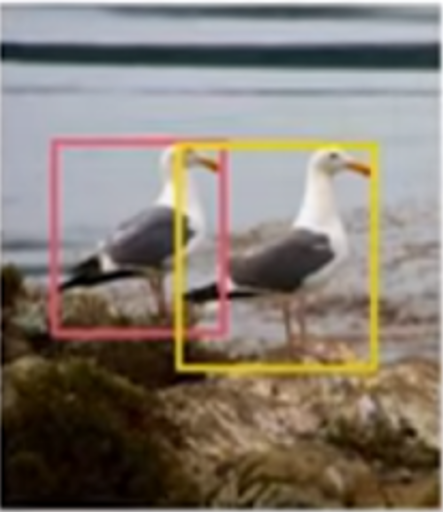
\includegraphics[keepaspectratio]{media/image2.png}}
\caption{Рис. 3.2 -- Схема технології трансформерів виявлення: а -- ЗНМ;
б -- кодер; в -- декодер; г -- НМПП}
\end{figure}

Для виявлення просторових ознак у ЗНМ застосовується вхідний шар для
зображень. У кодері який складається з декількох шарів, вхідні ознаки
перетворюються у високорівневі представлення. Декодер формує набір
обмежуючих рамок для передбачення виходів на основі представлень,
отриманих від кодера.

Розроблена модель декодера має вигляд{[}\hyperref[_Ref221290074]{57}{]}

\(B_{t} = \text{DETR}\left( I_{t} \right)\) (3.)

де F\_t -- кадр відеопослідовності; \(I_{t}\)

\(t\)t -- індекс кадру;

\(B_{t}\)B\_t -- набір обмежувальних рамок для кожного кадру.

Кожний кадр аналізується з використанням відео входу та детектора ТРВИ,
що дозволяє точно визначати положення та межі об'єктів у кадрі. Блок
оптичного потоку приймає вхідне зображення і генерує набір обмежуючих
рамок для кожного кадру

\({F_{t}}_{\rightarrow t + 1} = \text{OpticalFlow}\left( I_{t},I_{t + 1} \right)\)(3.2)

де I(t) та I(t+1) -- послідовні кадри; \(I_{t}I_{t + 1}\)

\(F_{t \rightarrow t + 1}\)F\_t -- поле оптичного потоку між цими
кадрами.

Алгоритми оптичного потоку застосовуються для визначення векторів руху
об'єктів між послідовними кадрами. Оптичний потік визначається як поле
векторів, що описує рух кожної точки кадру.

\(v = \frac{1}{N}\sum_{i = 1}^{N}{\parallel F_{t \rightarrow t + 1}(i) \parallel}\)(3.3)

де N -- кількість точок, що належать об'єкту; \(N\)

\(F_{t \rightarrow t + 1}\)v\_i -- вектор руху i-ї точки;

\(v\)v -- швидкість об'єкта;

\(\theta\)φ -- кут напрямку руху.

На основі отриманих векторів руху проводиться аналіз параметрів
об'єктів, включаючи швидкість та напрямок руху. Напрямок руху об'єкта
визначається, як середнє значення напрямків векторів руху. Швидкість
об'єкта розраховується як величина середнього вектору руху. Кут напрямку
руху об'єкта обчислюється за формулою

\(\theta = \frac{1}{N}\sum_{i = 1}^{N}{\text{atan2}\left( F_{t \rightarrow t + 1}^{y}(i),F_{t \rightarrow t + 1}^{x}(i) \right)}\)
(3.4)

Класична нейронна мережа з прямим поширенням обробляє вихід декодера для
отримання кінцевих результатів.

Завдяки застосуванню технології ТРВИ вдалося значно підвищити точність
виявлення об'єктів у відеопотоці, особливо в умовах складного фону та
динамічного середовища. Використання оптичного потоку дозволило точно
визначати параметри руху об'єктів, що є критично важливим для задач
реального часу, таких як системи безпеки, автономні транспортні засоби
та відеоспостереження 14; 45; 52.

Модель кодер -- декодер. Схема моделі з'єднання елементів кодер --
декодер показана на рис. 3.3. На рис. 3.3а наведено схему кодера, який
складається з шарів багатоголової самоуваги та НМПП\textbf{.}

На рис. 3.3б показано схему декодера, який має схожу структуру до кодера
з додатковими компонентами. Список шарів включає багатоголову самоувагу,
суму та нормування, багатоголову увагу (Multi-Head Attention), суму та
нормування, НМПП, де, як і в кодері, використовується багатошаровий
перцептрон {[}46; 53{]}.

Кодер -- це частина трансформера, яка приймає на вхід ознаки, що
отримані ЗНМ, та обробляє їх за допомогою механізмів багатоголової
самоуваги. Завдання кодера полягає в кодуванні вхідних ознак у
контекстні представлення, які зберігають інформацію про всі об'єкти в
сцені. Декодер приймає на вхід закодовані ознаки з кодера та
використовує механізми багатоголової уваги для визначення набору
фіксованих об'єктів. Виходом декодера є кінцеві координати та категорії
виявлених об'єктів.

На етапі попередньої обробки зображення ЗНМ витягує відповідні
просторові ознаки {[}44; 48{]}.

Трансформери мають мережеву архітектуру, що базується на механізмах
уваги для машинного перекладу. Маючи елемент запиту і набір ключових
елементів, багатоголовий модуль уваги адаптивно агрегує ключовий вміст з
відповідними вагами уваги, які вимірюють сумісність пар запит-ключ.
Елементом запиту може бути цільове слово у вихідному реченні, а набір
ключових елементів можуть складати вихідні слова у вхідному реченні.

\begin{figure}
\centering
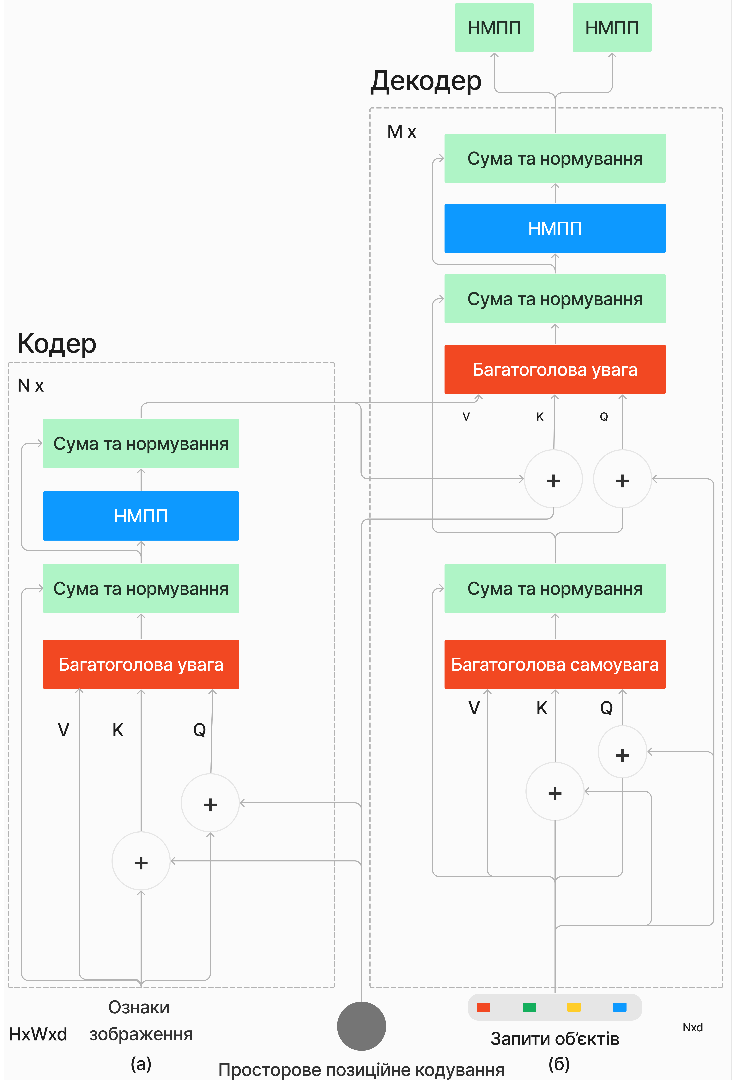
\includegraphics[width=6.10757in,height=8.98958in]{media/image3.png}
\caption{Рис. 3.3а -- Схема кодера трансформерної моделі DETR}
\end{figure}

Рис. 3.3б -- Схема декодера трансформерної моделі DETR

Щоб дозволити моделі фокусуватися на вмісті з різних підпросторів
представлення і з різних позицій, виходи різних голів уваги лінійно
агрегуються з перенавчальними важелями. Цей механізм забезпечує
трансформерам здатність визначати складні залежності між елементами
вхідних даних, що робить їх ефективними для широкого спектру задач
обробки природної мови та інших областей.

Функція багатоголової уваги обчислюється за
формулою{[}\hyperref[_Ref221573302]{49}{]}

\(\text{MultiHeadAttn}\left( z_{q},x \right) = \sum_{m = 1}^{M}{W_{m}\left\lbrack \sum_{k \in \Omega_{k}}^{}A_{mqk}*W_{m}'x_{k} \right\rbrack},\)
(3.5)

де q\_i -- індекс елемента запиту; \(q \in \Omega q\)

\(z_{q} \in \mathbb{R}^{C}\)x\_i\^{}q -- ознака представлення запиту;

\(m\)h -- індекс голови уваги;

\(M\)H -- кількість голів уваги;

\(W_{m} \in \mathbb{R}^{C \times C_{v}}\)W\^{}O -- вихідна проєкційна
матриця.

\(k \in \Omega k\)k\_j -- індекс елемента ключа;

\(A_{mqk}\)a\_ij\^{}h -- ваги уваги;

\(W_{m}^{’} \in \mathbb{R}^{C_{v} \times C}\)W\_h -- вхідна проєкційна
матриця для h-ї голови;

\(x_{k} \in \mathbb{R}^{C}\)x\_j\^{}k -- ознака представлення ключа;

\(\Omega q\)Q та K -- множини елементів запиту та ключа
відповідно.\(\Omega k\)

Вхідна та вихідна проєкції матриці мають перенавчальні важелі, що
визначаються розмірністю уваги для кожної голови уваги

\(C_{v}\  = \ C\text{/}M\)(3.6)

де d\_k -- розмірність ознаки ключа.\(C\)

Важелі уваги обчислюються за формулою

\(A_{mqk} \propto e^{\frac{z_{q}^{T}\ U_{m}^{T}\ V_{m}x_{k}}{\sqrt{C_{v}}}}\)(3.7)

де W\_h\^{}Q та W\_h\^{}K -- навчальні ваги вхідних запитів і ключів для
проєкції матриці на h-ту
голову;\(U_{m},V_{m} \in \mathbb{R}^{C_{v} \times C}m\)‑

\(m\)h, i та j -- індекси голови, запиту та ключа відповідно.\(qk\)

Важелі уваги нормалізуються за формулою

\(\sum_{k \in \Omega_{k}}^{}A_{mqk} = 1\)(3.8)

Ознаки представлення x\_i\^{}q та x\_j\^{}k зазвичай є конкатенацією або
сумою вмісту елементів та позиційних вкладок для розрізнення різних
просторових позицій.\(z_{q}x_{k}\)\-

Вектори запитів, ключів і значень обчислюються за формулами:

\(q_{i}\  = X_{i}W^{Q},\quad k_{i} = X_{i}W^{K},v_{i} = X_{i}W^{V}\)(3.9)

де X -- вхідний вектор або матриця вхідних векторів;\(X_{i}\)

\(W^{Q}\)W\^{}Q -- матриця ваг для перетворення в запити;

\(W^{K}\)W\^{}K -- матриця ваг для перетворення в ключі;

\(W^{V}\)W\^{}V -- матриця ваг для перетворення в значення;

\(q_{i}\)Q -- вектор або матриця запитів, отримана з вхідних ознак;

\(k_{i}\)K -- вектор або матриця ключів, отримана з вхідних ознак;

\(v_{i}\)V -- вектор або матриця значень, отримана з вхідних ознак.

Щоб обчислити ваги уваги і зважити відповідні значення створені вектори
запитів, ключів і значень використовуються в механізмі уваги з функцією

\(\text{Attention}\left( q_{i},k_{j},v_{j} \right)\text{ = }\sum_{j = 1}^{n}{\text{softmax}\left( \frac{q_{i} \cdot k_{j}}{\sqrt{d_{k}}} \right)v_{j}}\)(3.10)

де d\_k -- розмірність векторів ключів; \(d_{k}\)

\(K\)K -- матриця ключів;

\(k_{j}\)k\_j -- вектор-стовпець матриці ключів;

\(V\)V -- матриця значень;

\(v_{j}\)v\_j -- вектор-стовпець матриці значень.

Механізм уваги призначає ваги ключам на основі їх схожості з запитом. Ці
ваги використовуються для агрегування векторів значень у зважену суму,
яка потім використовується в моделі трансформера. Оцінки уваги
дозволяють моделі фокусуватися на різних частинах вхідної послідовності
для кожної вихідної позиції, що дозволяє захоплювати залежності
незалежно від їхньої відстані у послідовності. Увага цього типу
застосовується для взаємодії між різними части\-нами послідовностей в
трансформерних моделях. Вона розбиває вхідні дані на кілька голів, кожна
з яких використовується для відповідних обчислень. Кожна голова вивчає
взаємозв'язки між словами у різних контекстах та відповідності між
різними частинами послідовності.

Результати обчислень кожної голови конкатенуються та проходять через
додатковий проєктний шар перед об'єднанням для подальшої обробки.

Багатоголова самоувага у трансформерів -- це спеціалізований тип
багатоголової уваги, де вхідні дані подаються одночасно на всі голови
для обробки.

Кожна голова вивчає відносини між різними словами в межах цієї
послідовності за принципом самоподібності.

Цей підхід дозволяє моделі вивчати взаємозв'язки між різними частинами
послідовності без потреби у внутрішніх чи зовнішніх взаємодіях {[}4;
49{]}.

GeoNet. Глибока нейронна архітектура, яка поєднує задачу оцінки глибини
з задачею оцінки оптичного потоку , тобто векторного поля переміщення
пікселів між двома послідовними зображеннями. Її основна мета
інтегрувати просторову та часову інформацію в єдину структуру для більш
точної реконструкції сцени та відстеження об'єктів. У контексті задачі
ідентифікації параметрів динамічних об'єктів, GeoNet виступає як
фундаментальний інструмент для попереднього збору кінематичних
характеристик об'єктів у відеопотоці. показано загальну структуру
GeoNet, де пара вхідних зображень послідовних кадрів обробляється
мережею для одночасного визначення карти глибини та оптичного потоку.
Такий підхід дозволяє об'єднати стереозору та часову динаміку, що
критично важливо для ідентифікації просторового положення та напрямку
руху об'єктів у сцені. Використання GeoNet у поєднанні з трансформерною
архітектурою дозволяє значно підвищити точність визначення параметрів
руху завдяки можливості обробки глобального контексту у сцені
{[}\hyperref[_Ref221389746]{64}{]}. Трансформер аналізує отримані карти
глибини та оптичного потоку, забезпечуючи високорівневе представлення
руху, яке важливе для класифікації, прогнозування траєкторії та
подальшої аналітики об'єктів.

GeoNet може інтегруватись з ансамблевими методами машинного навчання,
зокрема в цій статті бегінгом та бустінгом, для підвищення стійкості до
шумів, зміни освітлення та часткової втрати даних. У випадку бегінгу,
GeoNet запропоновано виконувати на різних модифікованих підвибірках
відеокадрів, що дозволить отримати усереднені оцінки параметрів руху. У
бустінгу результати першої моделі аналізуються, і друга модель
фокусується на зонах з найбільшою похибкою, що забезпечує локальну
точність.

Таким чином, використання GeoNet у зв'язці з трансформерами та
ансамблевими підходами створює ефективну систему для високоточного
аналізу динаміки візуальних сцен та ідентифікації параметрів руху
об'єктів. Це особливо актуально в задачах дистанційного моніторингу,
автономного транспорту та систем відеоспостереження, де важлива не лише
фіксація наявності об'єкта, а й повноцінне розуміння його поведінки в
просторі.

Відео або зображення є проєкцією 3D-простору. 3D-сцена природно
складається зі статичного фону та об'єктів, що рухаються. Рух статичних
частин у відео викликаний виключно рухом камери та структурою глибини.
Тоді як рух динамічних об'єктів є більш складним, обумовленим як
однорідним рухом камери, так і специфічним рухом об'єкта.

\(f_{t \rightarrow s}^{rig}\left( p_{t} \right) = KT_{t \rightarrow s}D_{t}\left( p_{t} \right)K^{- 1}p_{t} - p_{t}\)
(3.11)

де K --- внутрішні параметри камери, p\_t --- однорідні координати
пікселів у кадрі I(t), T\_t→s --- відносний рух камери, D\_t --- карта
глибини.

\(\mathcal{L}_{rw} = \alpha\frac{1 - SSIM\left( I_{t},{\widetilde{I}}_{s}^{rig} \right)}{2} + (1 - \alpha)\| I_{t} - {\widetilde{I}}_{s}^{rig}\|_{1}\)
(3.12)

\(\mathcal{L}_{ds} = \sum_{p_{t}}^{}{|\nabla D(p_{t})| \cdot (e^{- \left| \nabla I\left( p_{t} \right) \right|})^{T}}\)
(3.13)

Перший етап забезпечує стереоскопічне сприйняття жорсткої структури
сцени, але ігнорує динамічні об'єкти. Тому ми пропонуємо другий
компонент --- ResFlowNet для локалізації нежорсткого руху.

\(\mathcal{L}_{ge} = \sum_{p_{t}}^{}{\lbrack\delta(p_{t})\rbrack \cdot \|\Delta f_{t \rightarrow s}^{full}(p_{t})\|_{1}}\)
(3.14)

\(\|\Delta f_{t \rightarrow s}^{full}(p_{t})\|_{2} < max\{\alpha,\beta\| f_{t \rightarrow s}^{full}(p_{t})\|_{2}\}\)
(3.15)

\(\mathcal{L} = \sum_{l}^{}{\sum_{\left\langle t,s \right\rangle}^{}\left\{ \mathcal{L}_{rw} + \lambda_{ds}\mathcal{L}_{ds} + \mathcal{L}_{fw} + \lambda_{fs}\mathcal{L}_{fs} + \lambda_{ge}\mathcal{L}_{ge} \right\}}\)
(3.16)

\subsection{3. Визначення параметрів методами оптичного
потоку}\label{ux432ux438ux437ux43dux430ux447ux435ux43dux43dux44f-ux43fux430ux440ux430ux43cux435ux442ux440ux456ux432-ux43cux435ux442ux43eux434ux430ux43cux438-ux43eux43fux442ux438ux447ux43dux43eux433ux43e-ux43fux43eux442ux43eux43aux443}

У підрозділі «3.3 Визначення параметрів методами оптичного потоку» для
подальшого викладу використано такі формульні залежності: (3.17),
(3.18), (3.19), (3.20), (3.21), (3.22), (3.23), (3.24), (3.25), (3.26),
(3.27), (3.28).

У підрозділі «3.3 Визначення параметрів методами оптичного потоку» для
подальшого викладу використано такі формульні залежності: (3.29),
(3.30), (3.31), (3.32), (3.33), (3.34), (3.35), (3.36), (3.37), (3.38),
(3.39), (3.40).

У підрозділі «3.3 Визначення параметрів методами оптичного потоку» для
подальшого викладу використано такі формульні залежності: (3.41),
(3.42), (3.43).

Опис використання оптичного потоку. Оптичний потік обчислюється між
двома зображеннями, prev\_frame\_gray та next\_frame\_gray, за допомогою
методу Farneback, який використовує параметри для покращення точності
виявлення руху. Параметри включають використання пірамідного масштабу
(0.5), трьох рівнів піраміди, вікно 15x15 пікселів для розрахунку
потоку, три ітерації уточнення, поліноміальне розширення з розміром
сусідства 5 пікселів, а також Гауссовий фільтр з відхиленням 1.2. Ці
налаштування дозволяють отримати більш точні результати для аналізу руху
об'єктів у відео, що важливо для відстеження динамічних об'єктів.

На рис. 3.4 показано результат використання оптичного потоку для
візуалізації напрямку та інтенсивності руху в кадрі .

\begin{figure}
\centering
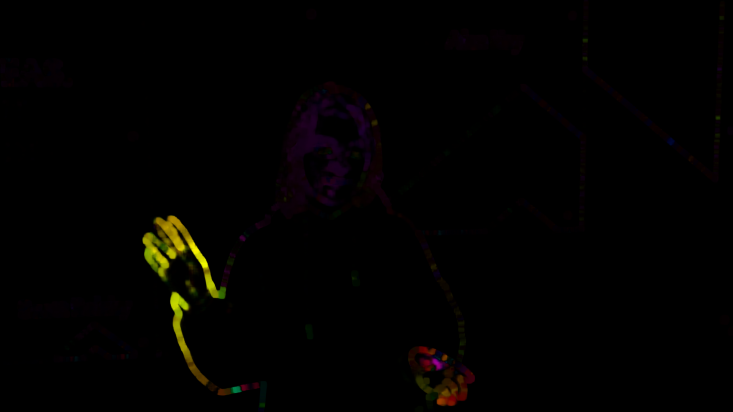
\includegraphics[width=6.16168in,height=5.02447in]{media/image4.png}
\caption{Рис. 3.4 -- Результат використання оптичного потоку для
візуалізації напрямку та інтенсивності руху}
\end{figure}

Оптичний потік, показаний на рис. 3.5 визначає напрям і швидкість
переміщення пікселів між послідовними кадрами. Його застосування
дозволяє отримати траєкторію руху об'єкта та визначити його кінематичні
параметри. Оптичний потік є векторним полем, яке відображає переміщення
пікселів між двома послідовними кадрами відео. Цей метод дозволяє
визначити напрямок і швидкість руху об'єктів у сцені. Завдяки цьому
можна побудувати траєкторію об'єкта, визначити його миттєву швидкість і
прискорення. У запропонованій системі оптичний потік виступає важливим
джерелом інформації про кінематичні параметри динамічних об'єктів,
особливо в ситуаціях, коли об'єкти частково або повністю перекриваються
(оклюзія) {[}54; 57{]}.

\begin{figure}
\centering
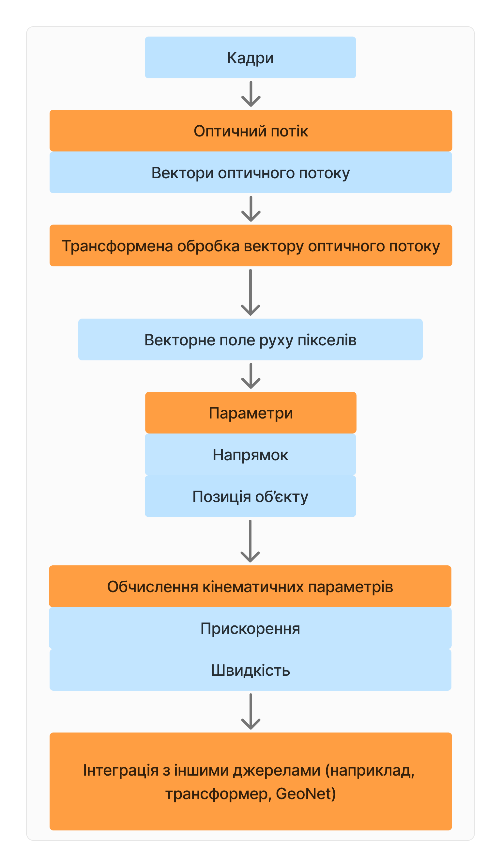
\includegraphics[width=5.47917in,height=9.48221in]{media/image5.png}
\caption{Рис. 3.5 -- Візуалізація оптичного потоку в обраній моделі}
\end{figure}

Метод оптичного потоку (Optical Flow) є фундаментальним інструментом у
галузі комп'ютерного зору, який забезпечує кількісне оцінювання руху
пікселів між послідовними кадрами відеопотоку. У межах розроблюваної
інформаційної технології дистанційної ідентифікації цей метод дозволяє
отримати детальну інформацію про динаміку сцени, що є критично важливим
для точного відстеження та розрахунку параметрів рухомих об'єктів у
реальному часі. Оптичний потік визначається як векторне поле, де кожен
вектор описує видиме переміщення точок зображення, що дає змогу
ідентифікувати швидкість, напрямок та траєкторію руху цілей без
безпосереднього фізичного контакту.

Традиційний аналіз руху базується на класичних диференціальних
алгоритмах, серед яких ключове місце посідають методи Лукаса--Канаде та
Хорна--Шунка 61; 62. Метод Лукаса--Канаде використовує локальне рівняння
різниці інтенсивності пікселів та метод найменших квадратів,
забезпечуючи високу швидкість обчислень при локальній сталості руху. На
противагу йому, метод Хорна--Шунка формулює задачу як мінімізацію
функціоналу енергії з умовою глобальної гладкості, що дозволяє будувати
густі карти руху, проте потребує значних ітераційних ресурсів та є
чутливим до шумів зображення.

Метод Горна--Шунка (Horn--Schunck) є глобальним методом обчислення
оптичного потоку, представленим у 1981 році. Він базується на двох
основних припущеннях: сталість яскравості означає, що колір або
яскравість точки об'єкта не змінюється між кадрами; плавність потоку
означає, що оптичний потік змінюється поступово від пікселя до пікселя.
На відміну від локального методу Лукаса--Канаде, який передбачає
сталість потоку в локальному вікні, метод Горна--Шунка є глобальним і
дає щільне поле оптичного потоку.

Основні припущення методу: сталість яскравості дозволяє порівнювати
пікселі між кадрами за рівнянням
\(I(x,\ y,\ t) = \ I(x\  + \ u\delta t,\ y\  + \ v\delta t,\ t\  + \ \delta t)\);
малий рух означає, що пікселі переміщуються лише на невелику відстань
між кадрами, що дозволяє лінеаризувати обмеження сталості яскравості.

\(I(x + u\delta t,y + v\delta t,t + \delta t) = I(x,y,t)\) (3.17)

Розклад в ряд Тейлора для малого δt:

\(I(x,y,t) + \frac{\partial I}{\partial x}\delta x + \frac{\partial I}{\partial y}\delta y + \frac{\partial I}{\partial t}\delta t = I(x,y,t)\)
(3.18)

Спрощення дає рівняння оптичного потоку:

\(I_{x}u + I_{y}v + I_{t} = 0\) (3.19)

де I\_x, I\_y --- просторові градієнти зображення, I(t) --- часова
похідна.

Метод поєднує два обмеження: сталість яскравості та плавність потоку.

\(E_{d}(i,j) = \left\lbrack {I_{x}u_{ij} + I_{y}v_{ij} + I_{t}} \right\rbrack^{2}\)
(3.20)

Складова плавності (smoothness) --- штрафує різкі зміни оптичного потоку
між сусідніми пікселями:

Повний функціонал, який мінімізується:

\({Min}_{u,v}\sum_{i,j}^{}\left\{ {E_{s}(i,j) + \lambda E_{d}(i,j)} \right\}\)
(3.21)

де λ --- параметр, що регулює вагу між гладкістю та відповідністю
яскравості.

\({\overline{u}}_{ij} = \frac{1}{4}\left( {u_{i + 1,j} + u_{i - 1,j} + u_{i,j + 1} + u_{i,j - 1}} \right)\)
(3.22)

Аналогічно для v̄\_ij.

\(\frac{\partial E}{\partial u_{kl}} = 2\left( u_{kl} - {\overline{u}}_{kl} \right) + 2\lambda\left( I_{x}u_{kl} + I_{y}v_{kl} + I_{t} \right)I_{x}\)
(3.23)

\(\frac{\partial E}{\partial v_{kl}} = 2\left( v_{kl} - {\overline{v}}_{kl} \right) + 2\lambda\left( I_{x}u_{kl} + I_{y}v_{kl} + I_{t} \right)I_{y}\)
(3.24)

Прирівнювання похідних до нуля дає систему лінійних рівнянь:

\(\left( 1 + \lambda I_{x}^{2} \right)u_{kl} + \lambda I_{x}I_{y}v_{kl} = {\overline{u}}_{kl} - \lambda I_{x}I_{t}\)
(3.25)

\[\lambda I_{x}I_{y}u_{kl} + \left( 1 + \lambda I_{y}^{2} \right)v_{kl} = {\overline{v}}_{kl} - \lambda I_{y}I_{t}\]

Це система вигляду Ax = b, яка розв'язується для кожного пікселя.

\(\left\{ 1 + \lambda\left( I_{x}^{2} + I_{y}^{2} \right) \right\} u_{kl} = \left( 1 + \lambda I_{x}^{2} \right){\overline{u}}_{kl} - \lambda I_{x}I_{y}{\overline{v}}_{kl} - \lambda I_{x}I_{t}\)
(3.26)

\(\left\{ 1 + \lambda\left( I_{x}^{2} + I_{y}^{2} \right) \right\} v_{kl} = \left( 1 + \lambda I_{y}^{2} \right){\overline{v}}_{kl} - \lambda I_{x}I_{y}{\overline{u}}_{kl} - \lambda I_{y}I_{t}\)
(3.27)

Після перетворень отримуємо ітераційну схему:

\({\widehat{u}}_{kl} = {\overline{u}}_{kl} - \frac{I_{x}{\overline{u}}_{kl} + I_{y}{\overline{v}}_{kl} + I_{t}}{\lambda^{- 1} + I_{x}^{2} + I_{y}^{2}}I_{x}\)
(3.28)

\({\widehat{v}}_{kl} = {\overline{v}}_{kl} - \frac{I_{x}{\overline{u}}_{kl} + I_{y}{\overline{v}}_{kl} + I_{t}}{\lambda^{- 1} + I_{x}^{2} + I_{y}^{2}}I_{y}\)
(3.29)

\(E_{s}(i,j) = \frac{1}{4}\left\lbrack {(u_{ij} - u_{i + 1,j})^{2} + (u_{ij} - u_{i,j + 1})^{2} + (v_{ij} - v_{i + 1,j})^{2} + (v_{ij} - v_{i,j + 1})^{2}} \right\rbrack\)
(3.30)

L₁ норма = Σ\textbar F(x+h) -- G(x)\textbar{}

L₂ норма = √(Σ{[}F(x+h) -- G(x){]}²)

Від'ємна нормована кореляція = -ΣF(x+h)G(x) / √(ΣF(x+h)² ΣG(x)²)

Для малих h лінійна апроксимація дає:

\(F'(x) \approx \frac{F(x + h) - F(x)}{h} = \frac{G(x) - F(x)}{h}\)
(3.31)

Отже:

\(h \approx \frac{G(x) - F(x)}{F'(x)}\) (3.32)

Усереднення декількох оцінок:

\(h = \sum_{x}^{}\frac{\frac{G(x) - F(x)}{F'(x)}}{\sum_{x}^{}1}\) (3.33)

Зважене усереднення з ваговою функцією
\(w(x) = \frac{1}{\left| G'(x) - F'(x) \right|}\):

\(h = \sum_{x}^{}\frac{\frac{w(x)\left\lbrack G(x) - F(x) \right\rbrack}{F'(x)}}{\sum_{x}^{}{w(x)}}\)
(3.34)

Ітерація Ньютона-Рафсона:

\(h_{0} = 0,h_{k + 1} = h_{k} + \sum_{x}^{}\frac{\frac{w(x)\left\lbrack G(x) - F\left( x + h_{k} \right) \right\rbrack}{F'\left( x + h_{k} \right)}}{\sum_{x}^{}{w(x)}}\)
(3.35)

Лінійна апроксимація:

\(F(x + h) \approx F(x) + hF'(x)\) (3.36)

Функція похибки:

\(E = \sum_{x}^{}{\lbrack F(x) + hF'(x) - G(x)\rbrack^{2}}\) (3.37)

Прирівнювання похідної до нуля дає:

\(h = \frac{\sum_{x}^{}{F'(x)\left\lbrack G(x) - F(x) \right\rbrack}}{\sum_{x}^{}{F'(x)^{2}}}\)
(3.38)

Для багатовимірного випадку мінімізуємо:

\(E = \sum_{x \in R}^{}{\lbrack F(x + h) - G(x)\rbrack^{2}}\) (3.39)

Лінійна апроксимація в n-вимірах:

\(F(x + h) \approx F(x) + h\frac{\partial F}{\partial x}\) (3.40)

Розв'язок для h:

\(h = \left\lbrack {\sum_{x}^{}{\left( \frac{\partial F}{\partial x} \right)^{T}\left( G(x) - F(x) \right)}} \right\rbrack\left\lbrack {\sum_{x}^{}{\left( \frac{\partial F}{\partial x} \right)^{T}\left( \frac{\partial F}{\partial x} \right)}} \right\rbrack^{- 1}\)
(3.41)

Узагальнений метод реєстрації може бути застосований для отримання
інформації про глибину зі стереопар зображень. Для об'єкта на відстані z
від камери 1, положення на площині плівки камери 2 може бути обчислено.
Використовуючи лінійну апроксимацію для корекції глибини Δz:

\(\Delta z = \sum_{x}^{}\frac{\frac{\partial F}{\partial z}\lbrack G - F\rbrack}{\sum_{x}^{}\left( \frac{\partial F}{\partial z} \right)^{2}}\)
(3.42)

де \(\frac{\partial F}{\partial z}\) обчислюється через правило ланцюга
з просторового градієнта інтенсивності та геометрії стереоустановки.
Аналогічно, для невідомих параметрів камери c, оновлення Δc має вигляд:

\(\Delta c = \left\lbrack {\sum_{x}^{}{\left( {\frac{\partial q}{\partial c}\frac{\partial F}{\partial q}} \right)^{T}(G - F)}} \right\rbrack\left\lbrack {\sum_{x}^{}{\left( {\frac{\partial q}{\partial c}\frac{\partial F}{\partial q}} \right)^{T}\left( {\frac{\partial q}{\partial c}\frac{\partial F}{\partial q}} \right)}} \right\rbrack^{- 1}\)
(3.43)

\[h = \sum_{x}^{}\frac{\frac{w(x)\left\lbrack G(x) - F(x) \right\rbrack}{F'(x)}}{\sum_{x}^{}{w(x)}}\]

Для практичної реалізації в інтелектуальних системах часто
використовується алгоритм Фарнбека (Farneback), який базується на
апроксимації інтенсивності пікселів поліномами. Цей метод використовує
пірамідальну структуру зображень, що дозволяє ефективно обробляти рухи
різних масштабів -- від повільних зміщень до швидких переміщень об'єктів
у кадрі. У розробленому програмному забезпеченні алгоритм Фарнбека
налаштований із використанням пірамідного масштабу 0.5, трьох рівнів
піраміди та Гауссового фільтра з відхиленням 1.2, що забезпечує високу
прецизійність ідентифікації кінематичних характеристик.

Сучасна еволюція методів аналізу руху призвела до появи нейромережевих
архітектур, таких як FlowNet та FlowNet 2.0, які навчаються передбачати
оптичний потік за принципом «кінець-у-кінець» (end-to-end). Модель
FlowNet пропонує два варіанти: FlowNetSimple, що самостійно вивчає рух
із пари зображень, та FlowNetCorr, яка використовує кореляційний шар для
явного порівняння областей кадрів. Використання великих синтетичних
наборів даних, як-от Flying Chairs, дозволяє цим моделям успішно
узагальнювати знання для ідентифікації параметрів руху в реальних
складних сценаріях.

FlowNet 2.0 суттєво вдосконалює цей процес завдяки архітектурі зі
стекуванням мереж та впровадженню спеціалізованих шарів для врахування
малих зміщень. Ця модель здатна обробляти дані зі швидкістю до 140
кадрів на секунду, що робить її ідеальним компонентом для автономних
транспортних систем та робототехніки. Висока деталізація та низька
похибка оцінки потоку у FlowNet 2.0 дозволяють точно ідентифікувати
навіть мінімальні зміни в стані динамічного об'єкта, що є критичним для
систем запобігання аваріям.

Інтеграція методів оптичного потоку з трансформерами виявлення (DETR)
створює синергетичний ефект у задачах дистанційної ідентифікації. У
такій комбінації DETR виконує прецизійну локалізацію об'єктів та
визначення їхніх меж, а блок Optical Flow обчислює вектори руху між
послідовними кадрами для цих локалізованих областей. Ця модель дозволяє
системі одночасно «бачити» об'єкт і «розуміти» фізику його переміщення,
що значно перевершує традиційні роздільні підходи за точністю та
стійкістю до динамічного фону.

На рис. 3.6 подано схему інтеграції оптичного потоку з трансформерною
обробкою векторів руху для подальшого визначення положення, швидкості,
прискорення та напряму руху динамічних об'єктів.

Рис. 3.6 -- Схема інтеграції оптичного потоку з трансформерною обробкою
параметрів руху

Математична модель оцінювання динамічних параметрів базується на аналізі
поля векторів руху \(F\). Швидкість об'єкта (\(v\)) розраховується як
величина середнього вектора руху для всіх точок (\(N\)), що належать
ідентифікованій цілі. Визначення миттєвої швидкості дозволяє системі
формувати динамічний профіль об'єкта в реальному часі. Такий підхід
забезпечує стабільність оцінок навіть при зміні форми об'єкта або його
частковому перекритті.

Для визначення траєкторії руху використовується розрахунок кута напрямку
(\(\theta\)) за допомогою функції atan2, яка аналізує вертикальні та
горизонтальні компоненти векторів зміщення пікселів. Середнє значення
напрямків усіх векторів руху об'єкта дозволяє точно спрогнозувати його
подальший шлях. Це є фундаментом для аналізу траєкторій в
інтелектуальних системах спостереження та автономного керування.

Ключовим аспектом інформаційної технології є переведення піксельних
зміщень у реальні фізичні величини (наприклад, км/год). Це досягається
через калібрування камери, що дозволяє системі ідентифікувати швидкість
транспортного засобу з похибкою не більше ±5 км/год. Такий рівень
точності задовольняє вимоги до систем моніторингу дорожнього руху та
промислової безпеки.

Для поглибленого просторового аналізу методи оптичного потоку
інтегруються з архітектурою GeoNet. GeoNet одночасно виконує монокулярну
оцінку глибини сцени та оптичного потоку, що дозволяє здійснювати
3D-реконструкцію динамічного середовища. Завдяки спільному навчанню
компонентів DepthNet та PoseNet, система здатна відокремлювати рух самої
камери від автономного руху об'єктів, що суттєво підвищує надійність
ідентифікації в рухомих системах (дрони, роботи).

Ефективність ідентифікації параметрів руху часто знижується через
оклюзії та зміни освітлення. Використання густого оптичного потоку
(Dense Optical Flow) допомагає нівелювати ці фактори, надаючи інформацію
про рух у кожній точці кадру, а не лише для окремих ознак. Це дозволяє
підтримувати безперервність відстеження об'єкта навіть у складних
міських умовах або при низькій якості відеозапису.

Для підвищення надійності оцінок використовуються ансамблеві методи,
такі як бегінг та бустінг. Бегінг дозволяє зменшити дисперсію
результатів через усереднення карт руху, отриманих на різних підвибірках
даних, що ефективно прибирає шумові артефакти. Бустінг застосовується
для послідовної корекції похибок у складних зонах, наприклад, на краях
рухомих тіл, де градієнти інтенсивності можуть бути розмитими.

Підсумовуючи, поєднання трансформерних моделей із алгоритмами оптичного
потоку та GeoNet забезпечує високу точність і адаптивність інформаційної
технології дистанційної ідентифікації. Отримані результати підтверджують
можливість надійного визначення швидкості та траєкторії динамічних
об'єктів у реальному часі. Подальший розвиток методології пов'язаний із
вдосконаленням систем підтримки прийняття рішень на основі
ідентифікованих характеристик руху для підвищення ефективності сучасних
«розумних систем».

\subsection{3.4 Об'єднання моделей і методів
ідентифікації}\label{ux43eux431ux454ux434ux43dux430ux43dux43dux44f-ux43cux43eux434ux435ux43bux435ux439-ux456-ux43cux435ux442ux43eux434ux456ux432-ux456ux434ux435ux43dux442ux438ux444ux456ux43aux430ux446ux456ux457}

На рис. 3.7 наведено узагальнену схему об'єднання відеопотоку, оптичного
потоку, трансформерної мережі та ансамблевого модуля для прогнозування
параметрів динамічних об'єктів.

Рис. 3.7 -- Узагальнена схема об'єднання моделей і методів ідентифікації

Порівняння однокрокових YOLO та двокрокових R-CNN методів детектування
свідчить про доцільність використання YOLO-подібних архітектур для
мобільних платформ завдяки їхній високій швидкості. Проте однокрокові
методи часто демонструють зниження ефективності при ідентифікації
дрібних та густо розташованих об'єктів. Впровадження моделей YOLOv11 та
YOLO-NAS дозволило частково нівелювати цей недолік за рахунок
використання квантізаційно-обізнаних модулів та автоматичного
проектування архітектури AutoNAC, що оптимізує баланс між затримкою та
пропускною здатністю системи.

Ефективність трансформерів виявлення DETR полягає у реалізації підходу
end-to-end, що усуває потребу в складних допоміжних компонентах, таких
як якірні рамки або механізм придушення не-максимумів NMS. Трансформери
забезпечують високу точність за рахунок моделювання глобальних
залежностей у всьому кадрі одночасно, що особливо важливо для стійкості
до часткових спотворень і перешкод. Хоча оригінальна модель DETR мала
тривалий час збіжності, модифікація Deformable DETR суттєво підвищила
продуктивність детектування малих об'єктів, досягнувши найкращих
результатів у своєму класі.

Аналіз методів оцінювання руху показав, що нейромережеві підходи, такі
як FlowNet 2.0, значно перевершують класичні алгоритми Лукаса--Канаде,
Хорна--Шунка за точністю та деталізацією. FlowNet 2.0 забезпечує
інтерактивну швидкість до 140 кадрів на секунду, що є критичним для
задач реального часу в автономному транспорті та системах безпеки.
Поєднання FlowNet із детекторами типу YOLO демонструє оптимальну
збалансованість точності та швидкості в умовах швидко змінюваних сцен,
тоді як зв'язка з DETR пріоритезує прецизійність результатів.

Інтеграція трансформерів та оптичного потоку створює синергетичний
ефект, де DETR виконує прецизійну локалізацію меж об'єктів, а Optical
Flow обчислює вектори руху саме для цих зон. Експериментальні
дослідження підтверджують, що така інтегрована модель значно перевершує
традиційні роздільні підходи у точності визначення параметрів об'єктів.
Це дозволяє надійно ідентифікувати швидкість і траєкторію руху в
реальному часі, що є фундаментом для створення інтелектуальних систем
моніторингу та керування.

Використання архітектури GeoNet додає системі можливість монокулярної
оцінки глибини, що перетворює 2D-аналіз на повноцінну 3D-реконструкцію
динамічної сцени. Ефективність GeoNet зумовлена спільним навчанням
компонентів DepthNet та PoseNet, що дозволяє точно розділяти рух самої
камери та автономний рух об'єктів. Це забезпечує ідентифікацію реальних
метричних відстаней, що є необхідною умовою для безпечного
функціонування робототехніки та безпілотних апаратів.

Ансамблевий метод бегінг довів свою ефективність у зниженні дисперсії
результатів ідентифікації. Виконання моделі GeoNet на різних випадкових
підвибірках або модифікаціях кадрів (зміна яскравості, кадрування) з
подальшим усередненням результатів дозволяє нівелювати вплив випадкових
шумів та артефактів. Такий підхід забезпечує стабільність глибинних карт
і векторів руху навіть за низької якості вхідного відеопотоку.

Ансамблевий метод бустінг демонструє високу ефективність у зменшенні
системного зміщення та уточненні параметрів у складних зонах зображення.
Послідовне навчання моделей, де спеціалізована нейромережа-коректор
фокусується на виправленні помилок попереднього етапу, дозволяє суттєво
підвищити точність на межах рухомих об'єктів. Зважене об'єднання
результатів бустінгу на основі локальних похибок гарантує прецизійну
локалізацію параметрів у зонах оклюзії або слабкої освітленості.

Впровадження підходів обчислювального інтелекту (CI), включаючи нечіткі
системи та еволюційні алгоритми, дозволяє розв'язувати
слабоформалізовані задачі в умовах невизначеності. Зокрема, поєднання
нечітких дерев рішень із бегінгом підвищує адаптивність системи до
розмитих або неповних даних, що властиво реальним процесам моніторингу.
Це забезпечує стабільну ідентифікацію станів об'єктів та можливість
самоналаштування регуляторів у режимі онлайн.

Ефективність програмної реалізації на Edge-пристроях (наприклад, NVIDIA
Jetson Nano) досягається через глибоку оптимізацію обчислювальних ядер.
Використання стратегії Liger-Kernel для злиття операцій GPU-ядер та
Triton-оптимізованих модулів дозволяє суттєво знизити затримки та
енергоспоживання. Це робить можливим виконання складних інтелектуальних
алгоритмів безпосередньо «на межі», забезпечуючи автономність прийняття
рішень без звернення до хмарних серверів.

Оптимізація пам'яті за допомогою моделей Neural Attention Memory Models
(NAMMs) дозволяє знизити використання KV-кешу трансформерів до 75\% без
втрати якості ідентифікації. Ефективність NAMMs полягає в адаптивному
відборі найбільш релевантних фрагментів контексту в довгих
відеопослідовностях, що запобігає переповненню пам'яті та деградації
швидкодії. Це дозволяє системі зосереджуватися на ключових змінах у
поведінці об'єктів, ігноруючи інформаційний шум.

Використання генеративних моделей (HunyuanVideo) та методів синтезу
даних (SynCamMaster) значно підвищує ефективність навчання систем
ідентифікації. SynCamMaster забезпечує геометричну узгодженість
синтетичного відео з різних точок огляду, що дозволяє створювати
реалістичні віртуальні навчальні вибірки для рідкісних або аварійних
сценаріїв. Це покращує здатність моделей до zero-shot transfer
(нульового переносу) на нові типи об'єктів та умови освітлення.

Для кількісного оцінювання якості ідентифікації параметрів динамічних
об'єктів у розробленій інформаційній технології застосовується система
метрик для оцінки точності оптичного потоку, глибини та якості
сегментації. Середня кінцева похибка EPE (End-Point Error) визначається
за формулою (4.17) і характеризує середню евклідову відстань між
передбаченим та істинним векторами руху:

Підсумовуючи аналіз ефективності, можна стверджувати, що інтегрована
модель, яка поєднує DETR, Optical Flow та GeoNet, є найбільш дієвим
інструментом для ДІПДО. Результати тестування на складних відеозаписах
підтвердили високу стійкість системи до зміни освітлення, шумів та
оклюзій. Досягнута точність детектування понад 90\% та низька похибка
оцінки динамічних характеристик роблять цю технологію перспективною для
впровадження в автономні транспортні системи, робототехніку та
промислову автоматизацію України.

\subsection{3.5 Висновки до
розділу}\label{ux432ux438ux441ux43dux43eux432ux43aux438-ux434ux43e-ux440ux43eux437ux434ux456ux43bux443-2}

У розділі 3 сформовано концепцію моделей дистанційної ідентифікації
параметрів динамічних об'єктів, розглянуто моделі ідентифікації за
відеоданими, методи оптичного потоку та підходи до об'єднання моделей.
Показано, що інтеграція DETR, Optical Flow, GeoNet і ансамблевих методів
дає змогу підвищити точність локалізації, оцінювання швидкості, напряму
руху та просторового положення об'єктів.

Запропоновані моделі забезпечують перехід від покадрового виявлення до
просторово-часового опису динамічного об'єкта. Вони поєднують координати
та межі об'єкта, вектори оптичного потоку, карти глибини і результати
трансформерного аналізу, що дозволяє отримати більш повний набір
параметрів для систем керування та підтримки прийняття рішень.

Порівняльний аналіз підтвердив, що використання ансамблевої агрегації та
моделей просторово-часової пам'яті підвищує стійкість ідентифікації в
умовах шумів, оклюзій і зміни освітлення. Отримані результати стали
основою для програмної реалізації інформаційної технології та
експериментального тестування в розділі 4.

\section{\texorpdfstring{Розділ 4 ІНФОРМАЦІЙНА ТЕХНОЛОГІЯ ДИСТАНЦІЙНОЇ
ІДЕНТИФІКАЦІЇ ПАРАМЕТРІВ ДИНАМІЧНИХ ОБ'ЄКТІВ\\
}{Розділ 4 ІНФОРМАЦІЙНА ТЕХНОЛОГІЯ ДИСТАНЦІЙНОЇ ІДЕНТИФІКАЦІЇ ПАРАМЕТРІВ ДИНАМІЧНИХ ОБ'ЄКТІВ }}\label{ux440ux43eux437ux434ux456ux43b-4-ux456ux43dux444ux43eux440ux43cux430ux446ux456ux439ux43dux430-ux442ux435ux445ux43dux43eux43bux43eux433ux456ux44f-ux434ux438ux441ux442ux430ux43dux446ux456ux439ux43dux43eux457-ux456ux434ux435ux43dux442ux438ux444ux456ux43aux430ux446ux456ux457-ux43fux430ux440ux430ux43cux435ux442ux440ux456ux432-ux434ux438ux43dux430ux43cux456ux447ux43dux438ux445-ux43eux431ux454ux43aux442ux456ux432}

У четвертому розділі описано структуру та програмну реалізацію
інформаційної технології дистанційної ідентифікації параметрів
динамічних об'єктів. Наведено результати експериментального поєднання
трансформерів, методів оптичного потоку, оцінювання глибини та
ансамблевих підходів, а також виконано аналіз ефективності отриманих
рішень.

\subsection{4. Структура інформаційної технології дистанційної
ідентифікації}\label{ux441ux442ux440ux443ux43aux442ux443ux440ux430-ux456ux43dux444ux43eux440ux43cux430ux446ux456ux439ux43dux43eux457-ux442ux435ux445ux43dux43eux43bux43eux433ux456ux457-ux434ux438ux441ux442ux430ux43dux446ux456ux439ux43dux43eux457-ux456ux434ux435ux43dux442ux438ux444ux456ux43aux430ux446ux456ux457}

Розроблена інформаційна технологія ДІПДО є комплексним підходом до
аналізу динамічних об'єктів у відеопотоках. Загальна модифікована
структура GeoNet, яка лягла в основу запропонованої технології, наведена
на рис. 4.. Оригінальний GeoNet включає компоненти оцінки глибини
(DepthNet), оцінки пози (PoseNet), оцінки оптичного потоку (ResFlowNet)
і працює без вчителя (unsupervised). У запропонованій модифікації додано
нові елементи: трансформер, що моделює просторово-часові залежності
(Transformer dynamic flow), ансамблеві методи для підвищення точності
(Ensemble methods), а також розширений підхід до трекінгу параметрів
(швидкість, напрямок руху тощо\hl{). Показано на рис. 4.1 загальну
модифіковану структуру} \hl{GeoNet}. \hl{На рис. 4.1 присутні нові
елементи, яких немає в оригінальній роботі трансформер, що моделює
просторово-часові залежності (Transformer dynamic flow), згадки про
бустінг/бегінг для підвищення точності (Ensemble methods), більш
загальний підхід до трекінгу параметрів (швидкість, напрямок руху тощо),
що виходить за межі задач (GeoNet Predicts the parameters), наявність
блоків (Transformer parameters, Opical flow information) з підключенням
до ансамблевих методів також свідчить про спроба об'єднати класичні
компоненти (оптичний потік, геометрія), трансформери (для глобального
контексту), та ансамблеві методи (для підвищення точності).}

Рис. 4. ̶ Модифікована структура GeoNet

На рис. 4.2, 4.3 показано етапи аналізу вхідних даних з відео, сенсорів
та зображень, які проходять через модулі попередньої обробки, виділення
ознак, оптичного потоку, оцінювання глибини, ідентифікації параметрів та
формування результатів.\hyperref[_Ref226899803]{3}

Рис. 4. -- Загальна схема обробки сигналів та ідентифікація об'єктів

На рис. 4.3 деталізовано структуру обробки сигналів та ідентифікації
об'єктів із урахуванням модулів оптичного потоку, оцінювання глибини,
виділення ознак і формування результатів.

Рис. 4. -- Обробка сигналів та ідентифікація об'єктів

У табл. 4.1 наведено методи визначення основних параметрів динамічних
об'єктів та відповідні абсолютні
похибки.\hyperref[_Ref221399609]{Таблиця 4.1 -- Методи визначення
ідентифікації параметрів динамічних об'єктів1}

У табл. 4.1 також узагальнено параметри положення, швидкості,
прискорення та орієнтації, а також методи їх визначення в межах
запропонованої інформаційної технології.\hyperref[_Ref221399609]{Таблиця
4.1 -- Методи визначення ідентифікації параметрів динамічних
об'єктів1}\hyperref[_Ref226482723]{Таблиця 4.2 -- Умови та склад
програмного експерименту1}

\begin{longtable}[]{@{}
  >{\raggedright\arraybackslash}p{(\linewidth - 2\tabcolsep) * \real{0.2445}}
  >{\raggedright\arraybackslash}p{(\linewidth - 2\tabcolsep) * \real{0.4181}}@{}}
\caption{\protect\phantomsection\label{_Ref221399609}{}Таблиця 4.1 --
Методи визначення ідентифікації параметрів динамічних
об'єктів1}\tabularnewline
\toprule\noalign{}
\begin{minipage}[b]{\linewidth}\raggedright
Параметр
\end{minipage} & \begin{minipage}[b]{\linewidth}\raggedright
Метод визначення
\end{minipage} \\
\midrule\noalign{}
\endfirsthead
\toprule\noalign{}
\begin{minipage}[b]{\linewidth}\raggedright
Параметр
\end{minipage} & \begin{minipage}[b]{\linewidth}\raggedright
Метод визначення
\end{minipage} \\
\midrule\noalign{}
\endhead
\bottomrule\noalign{}
\endlastfoot
Положення & Stereo Triangulation \\
Швидкість & Optical Flow + Kalman Filter \\
Прискорення & IMU Sensor Fusion \\
Орієнтація & Quaternion from EMG \\
\end{longtable}

\subsection{4. Програмна реалізація моделей дистанційної
ідентифікації}\label{ux43fux440ux43eux433ux440ux430ux43cux43dux430-ux440ux435ux430ux43bux456ux437ux430ux446ux456ux44f-ux43cux43eux434ux435ux43bux435ux439-ux434ux438ux441ux442ux430ux43dux446ux456ux439ux43dux43eux457-ux456ux434ux435ux43dux442ux438ux444ux456ux43aux430ux446ux456ux457}

На рис. 4.4 показано реалізовану модель, яка включає обробку
відеопотоку, використання моделі DETR, використання оптичного потоку,
формування і відображення результатів. Кольорами відмічено різні
елементи реалізованої моделі.

Рис. 4.4 -- Реалізована модель

На рис. 4. показано розширений опис реалізованої моделі. Яка включає
наступні елементи у вигляді конвеєру:

1. Обробку відео потоку. Збереження відео файлу з відеопотоку.
Екстракція кадрів з відеофайлу. Отримання кадрів з відео файлу для
подальшої їх обробки.

2. Модель DETR. Кожен кадр обробляється моделлю для виявлення об'єктів,
тобто виділення обмежувальних рамок об'єктів знайдений на кадрах.
Отримання кадрів з рамками.

3. Обчислення оптичного потоку. Визначення векторів руху. Аналіз
швидкості та напрямку. Отримання візуалізації руху.

Рис. 4.5 -- Розширений опис реалізованої моделі

\subsection{4. Програмна реалізація з використанням ансамблевих
методів}\label{ux43fux440ux43eux433ux440ux430ux43cux43dux430-ux440ux435ux430ux43bux456ux437ux430ux446ux456ux44f-ux437-ux432ux438ux43aux43eux440ux438ux441ux442ux430ux43dux43dux44fux43c-ux430ux43dux441ux430ux43cux431ux43bux435ux432ux438ux445-ux43cux435ux442ux43eux434ux456ux432}

Для підвищення надійності ідентифікації в умовах динамічної зміни
середовища застосовуються ансамблеві методи машинного навчання.
Структура ансамблевих модулів у системі наведена на рис. 4..

Рис. 4.6 -- Структура ансамблевих модулів у системі

На рис. 4.6 наведено результат «Структура ансамблевих модулів у
системі», який використовується для порівняння оптичного потоку, карти
глибини та об'єднаного представлення сцени під час дистанційної
ідентифікації параметрів динамічних об'єктів.

Для бегінгу об'єднання карт глибини методом середнього значення. Для
бегінгу карти глибини, отримані з різних підвибірок кадрів, об'єднуються
шляхом усереднення. Це дозволяє згладити локальні артефакти та підвищити
стабільність результатів.

Для бустінгу зважене об'єднання результатів з урахуванням локальних
похибок (приклад використання нейронної мережі-коректора). Для бустінгу
застосовується зважене об'єднання результатів, де ваги призначаються на
основі локальної похибки кожної моделі. У разі значного відхилення
результатів у певній області рішення приймається на користь тієї моделі,
яка показала нижчу похибку у сусідніх регіонах. Для цього
використовується нейронна мережа-коректор.

\subsection{4. Результат поєднання трансформерів і методів оптичного
потоку}\label{ux440ux435ux437ux443ux43bux44cux442ux430ux442-ux43fux43eux454ux434ux43dux430ux43dux43dux44f-ux442ux440ux430ux43dux441ux444ux43eux440ux43cux435ux440ux456ux432-ux456-ux43cux435ux442ux43eux434ux456ux432-ux43eux43fux442ux438ux447ux43dux43eux433ux43e-ux43fux43eux442ux43eux43aux443}

Для демонстрації роботи розробленої інформаційної технології було
проведено серію експериментів на тестових відеоданих. На рис. 4.
наведено результати роботи моделі DETR (Detection Transformer) для
виявлення об'єктів у кадрі.

У межах цього підрозділу виконано порівняння комбінованих схем за
однаковою логікою оброблення: спочатку формується поле оптичного потоку,
далі оцінюється карта глибини, після чого результати накладаються на
зображення кадру для подальшої інтерпретації. Такий підхід дає змогу
зіставити класичні та нейромережеві алгоритми за стабільністю,
деталізацією та здатністю зберігати просторову структуру сцени.

Для аналізу враховано якість виявлення об'єктів, узгодженість напрямку
руху, чіткість меж на карті глибини, стійкість до шумів і придатність
результату до подальшого використання в модулі ідентифікації. Саме тому
далі наведено окремі результати для Farneback, FlowNet, GeoNet,
Horn-Schunck і Lucas-Kanade у поєднанні з різними моделями оцінювання
глибини.

Отримані візуалізації не дублюють одна одну, а відображають різні режими
роботи інформаційної технології: від базового оптичного потоку й простих
способів оцінювання глибини до інтегрованих схем, у яких поєднуються
виявлення, рух і просторова інтерпретація кадру. Саме тому кожен
наступний підрозділ акцентує окремий тип комбінації та його практичну
інтерпретацію.

\begin{figure}
\centering
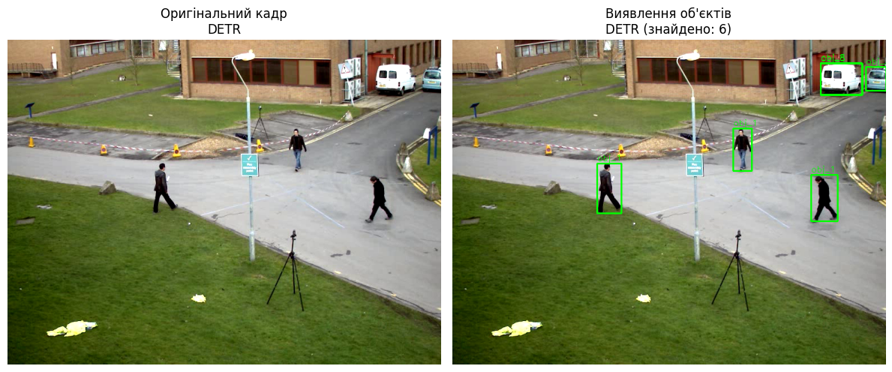
\includegraphics[width=6.68867in,height=2.79023in]{media/image6.png}
\caption{Рис. 4.7 -- Результат виявлення об'єктів за допомогою моделі
DETR}
\end{figure}

\hl{На рис. 4.7 модель DETR успішно локалізує об'єкти в кадрі, виділяючи
їх обмежувальними рамками. Виявлено 6 об'єктів, що відповідає реальній
кількості рухомих цілей у сцені. На рис. 4.8 показано візуалізацію
обчислених параметрів для виявлених об'єктів, а саме: їх просторового
положення (x, y, z), миттєвої швидкості та напрямку руху}.

\begin{figure}
\centering
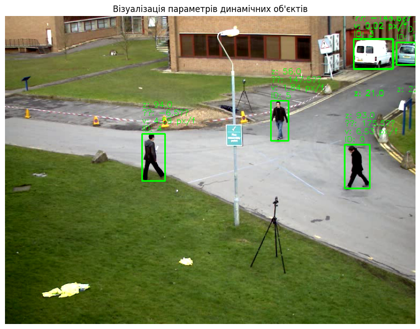
\includegraphics[width=6.28407in,height=4.91667in]{media/image7.png}
\caption{Рис. 4.8 -- Візуалізація ідентифікованих параметрів об'єктів}
\end{figure}

Подальший аналіз показав, що комбінування різних методів оцінки
оптичного потоку та глибини дає різні результати. На рис. 4.9 показано
приклад роботи системи з використанням алгоритму оптичного потоку
Фарнбека (Farneback) для оцінки руху та моделі MiDaS для оцінки глибини
сцени. Це класичний підхід Farneback + MiDaS.

\begin{figure}
\centering
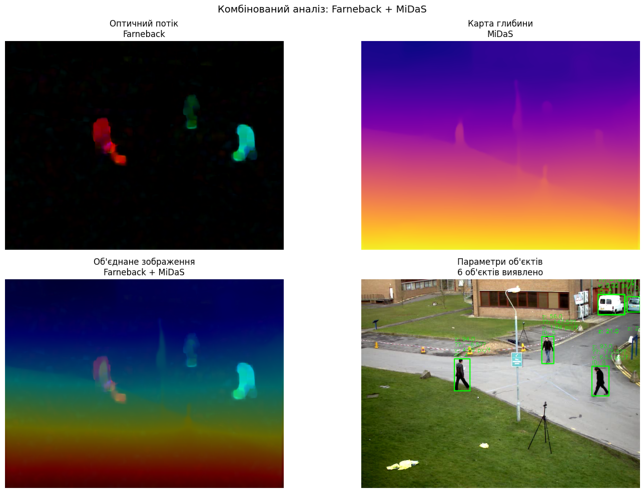
\includegraphics[width=6.31657in,height=4.83436in]{media/image8.png}
\caption{Рис. 4.9 -- Візуалізація оптичного потоку (Farneback), карти
глибини (MiDaS) та їх об'єднання}
\end{figure}

На рис. 4.9 зліва показано поле оптичного потоку, де кольором закодовано
напрямок та інтенсивність руху пікселів. У центрі представлено карту
глибини, отриману за допомогою моделі MiDaS, де теплі кольори (жовтий,
помаранчевий) відповідають ближчим об'єктам, а холодні (синій,
фіолетовий) -- віддаленим. Справа наведено результат об'єднання цих
даних, що дозволяє одночасно аналізувати як динаміку, так і просторову
структуру сцени. REF \_Ref

Аналогічний аналіз було проведено для пари «нейромережевий оптичний
потік FlowNet + DPT\_Large». Результати цього експерименту наведено на
рис.~4..

\begin{figure}
\centering
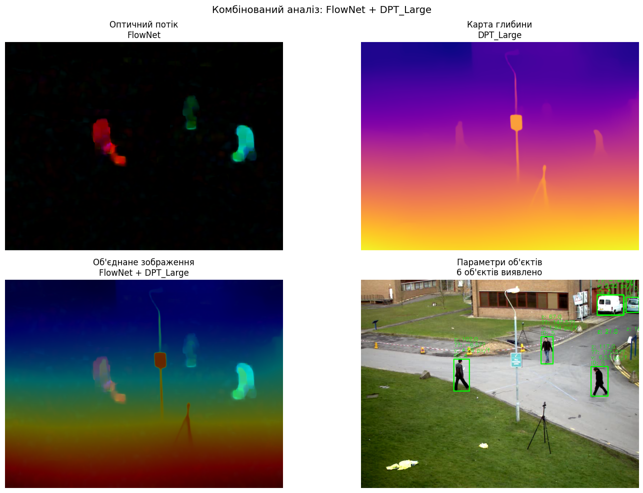
\includegraphics[width=6.41912in,height=4.91667in]{media/image9.png}
\caption{Рис. 4.10 -- Візуалізація оптичного потоку (FlowNet), карти
глибини (DPT\_Large) та їх об'єднання}
\end{figure}

На рис. 4.10 використання нейромережевих методів (FlowNet) дозволяє
отримати більш деталізоване поле оптичного потоку порівняно з класичним
алгоритмом Фарнбека, особливо на межах об'єктів. Оцінка глибини за
допомогою DPT\_Large також демонструє вищу роздільну здатність.
Використання FlowNet дає більш деталізоване поле оптичного потоку,
особливо на межах об'єктів (артефакти руху зменшуються). DPT\_Large
забезпечує вищу роздільну здатність карти глибини порівняно з MiDaS, що
дозволяє розрізняти об'єкти на різних відстанях з більшою точністю.

Інтегральний підхід GeoNet, який одночасно оцінює глибину та оптичний
потік, показав себе як ефективний інструмент для спільного аналізу (рис.
4.11). Результати демонструють узгодженість між просторовою та часовою
інформацією: рухомі об'єкти чітко відокремлюються від статичного фону, а
їх просторове положення узгоджується з картою глибини.

\begin{figure}
\centering
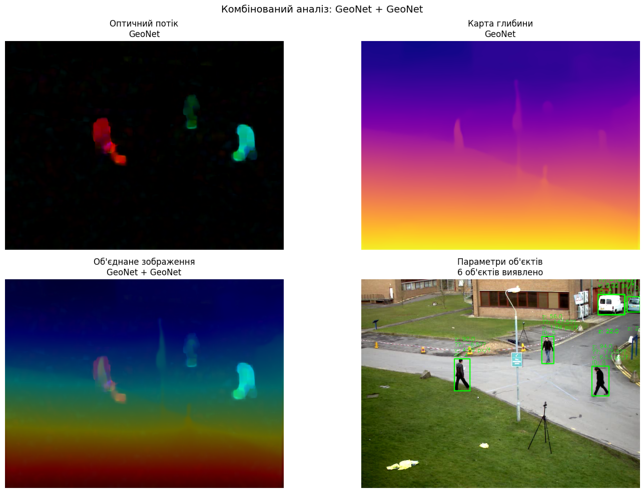
\includegraphics[width=6.54661in,height=5.01042in]{media/image10.png}
\caption{Рис. 4.11 -- Візуалізація результатів роботи інтегрованої
моделі GeoNet}
\end{figure}

Для підвищення стійкості ідентифікації до шумів було застосовано
ансамблевий метод бегінгу (Bagging). На рис. 4.12 представлено результат
роботи системи, де для оцінки глибини використовується ансамбль моделей
(Bagging), а оптичний потік обчислюється методом Горна--Шунка
(HornSchunck).

\begin{figure}
\centering
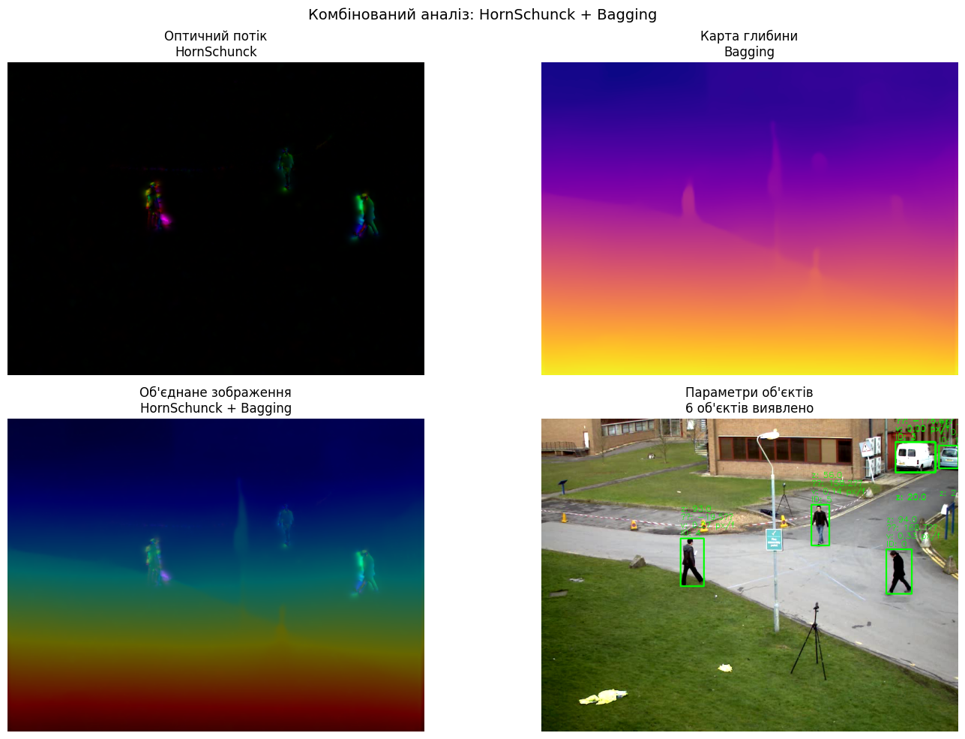
\includegraphics[width=6.54787in,height=5.01138in]{media/image11.png}
\caption{Рис. 4.12 -- Візуалізація оптичного потоку (HornSchunck) та
ансамблевої оцінки глибини (Bagging)}
\end{figure}

Завершальним етапом є інтеграція модуля виявлення об'єктів (DETR) з
модулем оцінки руху (Optical Flow). Як показано На рис. 4.13
обмежувальні рамки, отримані від DETR, накладаються на візуалізацію
оптичного потоку. Це дозволяє для кожного виявленого об'єкта обчислити
його індивідуальні параметри руху, такі як швидкість та напрямок.

\begin{figure}
\centering
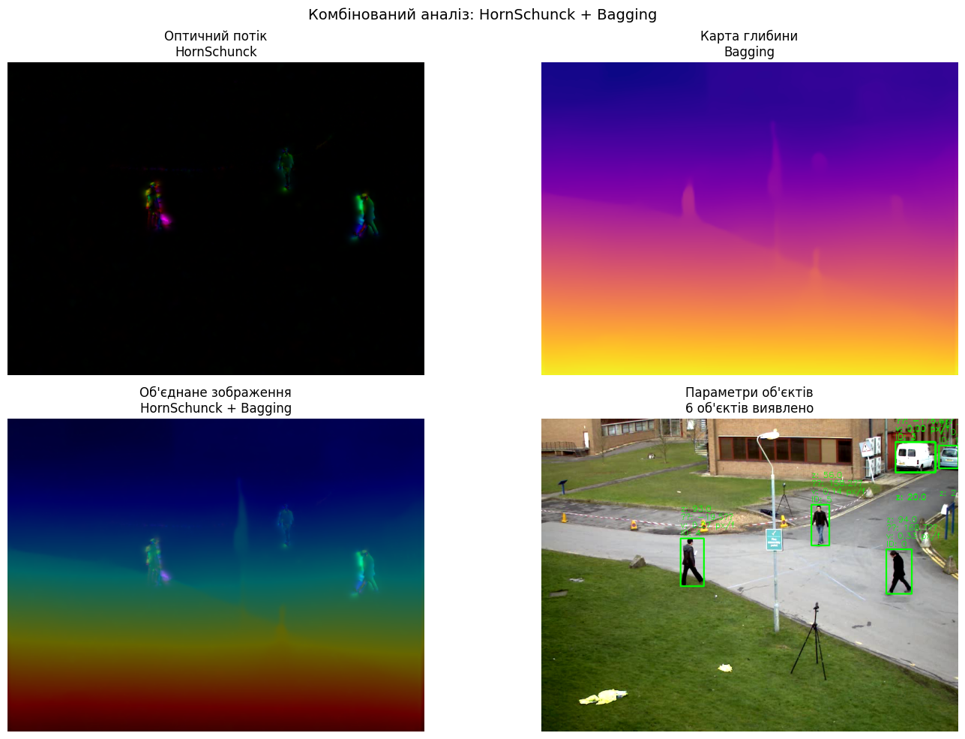
\includegraphics[width=6.54787in,height=5.01138in]{media/image11.png}
\caption{Рис. 4.13 -- Результат інтеграції моделі виявлення DETR з
візуалізацією оптичного потоку}
\end{figure}

На рис. 4.14--4.26 показано результати візуалізації оптичного потоку та
карти глибини після об'єднання. Результати отримані за допомогою
розробленого застосунку, у якому завантажується приклад відео з
бібліотеки OpenCV, вибираються два кадри, обчислюється карта глибини,
розраховується оптичний потік, а потім обидві карти візуалізуються
окремо та накладаються в одному зображенні.

На рисунку показано результати комплексної обробки відеоданих із
використанням методів оцінки оптичного потоку, побудови карти глибини та
їх подальшого об'єднання. Ліва частина зображення демонструє поле
оптичного потоку, де рухомі об'єкти виділено кольоровими маркерами на
темному фоні. Інтенсивність і напрямок руху закодовано у вигляді
кольорових відтінків, що дозволяє чітко ідентифікувати динамічні
елементи сцени, зокрема пішоходів, які переміщуються у різних напрямках.

Центральна частина зображення відображає карту глибини сцени, отриману
за допомогою відповідного алгоритму оцінки відстані до об'єктів.
Кольорова шкала використовується для представлення відносної
віддаленості: теплі кольори (жовтий, помаранчевий) відповідають ближчим
об'єктам, тоді як холодні (фіолетовий, синій) більш віддаленим. Такий
підхід забезпечує наочне сприйняття просторової структури сцени та
дозволяє оцінити розташування об'єктів у тривимірному просторі навіть за
наявності лише двовимірного зображення.

Права частина зображення демонструє результат об'єднання оптичного
потоку та карти глибини, що формує узагальнене представлення сцени. У
цьому випадку рухомі об'єкти не лише виділяються за рахунок динамічних
характеристик, але й доповнюються інформацією про їхню відстань від
камери. Така інтеграція даних підвищує інформативність аналізу, дозволяє
більш точно сегментувати об'єкти та створює передумови для подальшої
інтелектуальної обробки, зокрема ідентифікації параметрів динамічних
об'єктів і прийняття рішень у системах комп'ютерного зору.

\begin{figure}
\centering
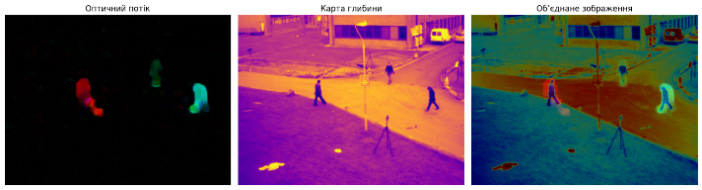
\includegraphics[width=6.51142in,height=1.76042in]{media/image12.png}
\caption{Рис. 4.14 -- Результат візуалізації оптичного потоку та карти
глибини після об'єднання}
\end{figure}

На рис. 4.14, 4.15 ліва панель демонструє поле оптичного потоку,
отримане методом Фарнбека. Кольорова гама показує напрямки руху:
червоно-жовті відтінки відповідають руху вправо, синьо-зелені вліво.
Центральна панель карта глибини, отримана простим розмиттям (Blur).
Теплі тони (жовтий/помаранчевий) відповідають ближнім об'єктам (умовно
0--50), холодні (синій/фіолетовий) -- віддаленим (100+). Видно, що Blur
дає лише дуже приблизну оцінку глибини: межі об'єктів розмиті, відсутня
деталізація. Права панель об'єднання: кольорові вектори потоку
накладаються на розмиту карту глибини. Така комбінація непридатна для
практичного використання через надто низьку якість оцінки
глибини.\hyperref[_Ref226405291]{14}\hyperref[_Ref226802991]{15}

\begin{figure}
\centering
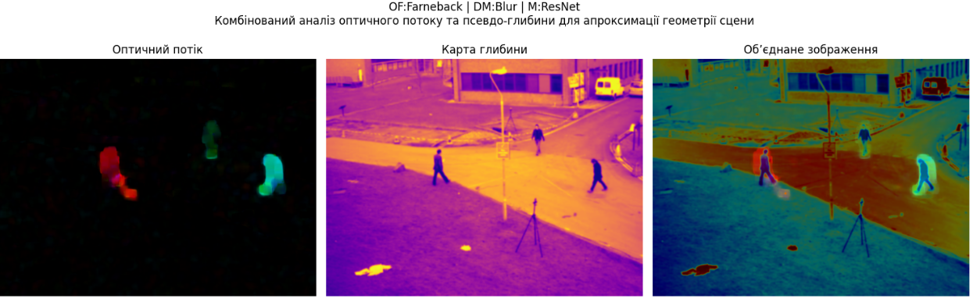
\includegraphics[width=6.59653in,height=2.10877in]{media/image13.png}
\caption{Рис. 4.15 -- Результат візуалізації оптичного потоку та карти
глибини після об'єднання Farneback + Blur}
\end{figure}

На рис. 4.15 наведено результат «Результат візуалізації оптичного потоку
та карти глибини після об'єднання Farneback + Blur», який
використовується для порівняння оптичного потоку, карти глибини та
об'єднаного представлення сцени під час дистанційної ідентифікації
параметрів динамічних об'єктів.

На рис. 4.16 наведено результат поєднання Farneback з градієнтною
оцінкою глибини.\hyperref[_Ref226809873]{16}

\begin{figure}
\centering
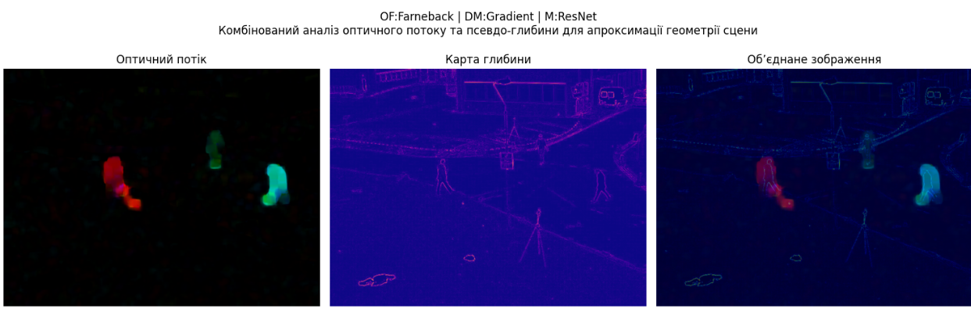
\includegraphics[width=6.46114in,height=2.1in]{media/image14.png}
\caption{Рис. 4.16 -- Результат візуалізації оптичного потоку та карти
глибини після об'єднання Farneback + Gradient}
\end{figure}

На рис. 4.17 наведено результат поєднання Farneback з моделлю MiDaS.

\begin{figure}
\centering
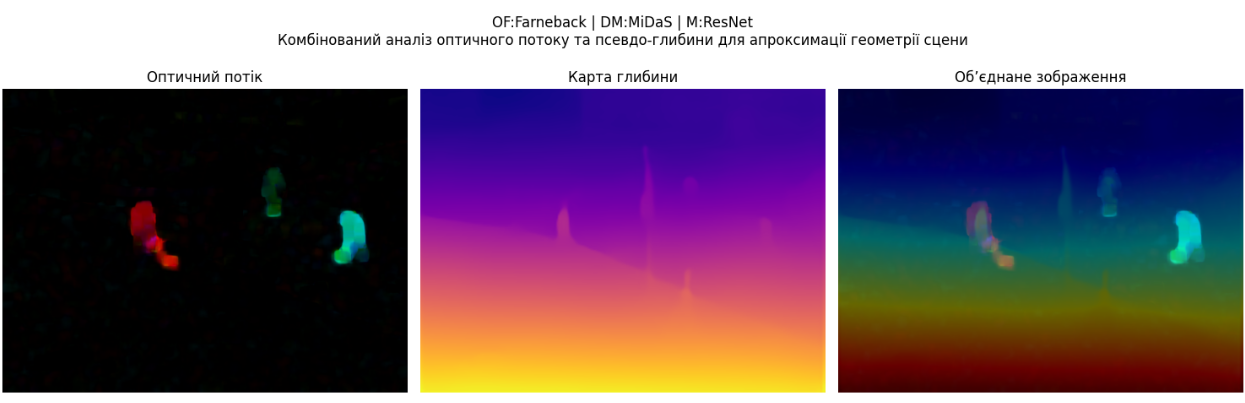
\includegraphics[width=6.38462in,height=2.06667in]{media/image15.png}
\caption{Рис. 4.17 -- Результат візуалізації оптичного потоку та карти
глибини після об'єднання Farneback + MiDaS}
\end{figure}

На рис. 4.18 наведено результат поєднання Farneback з моделлю
DPT\_Large.

\begin{figure}
\centering
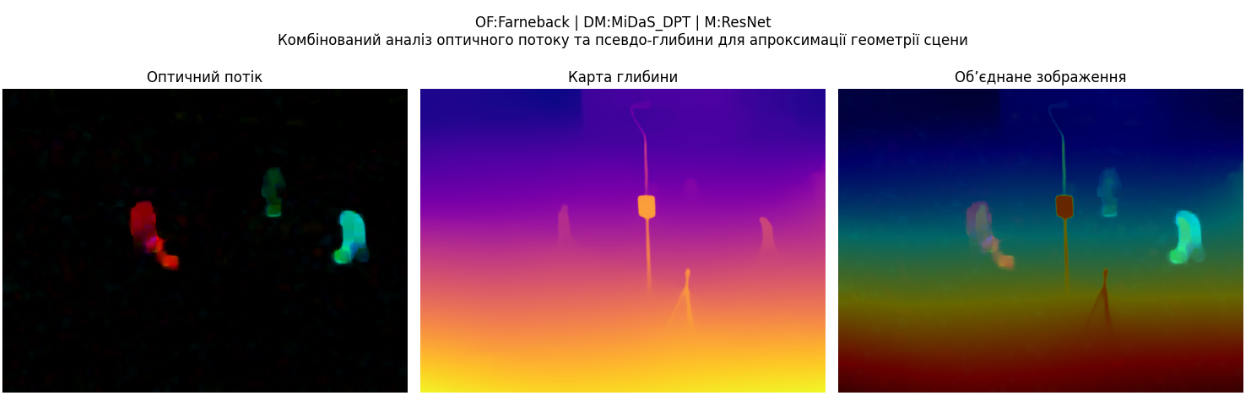
\includegraphics[width=6.33255in,height=2.05833in]{media/image16.png}
\caption{Рис. 4.18 -- Результат візуалізації оптичного потоку та карти
глибини після об'єднання Farneback + DPT\_Large}
\end{figure}

На рис. 4.19 наведено результат поєднання Lucas--Kanade з розмиттям
карти глибини.

\begin{figure}
\centering
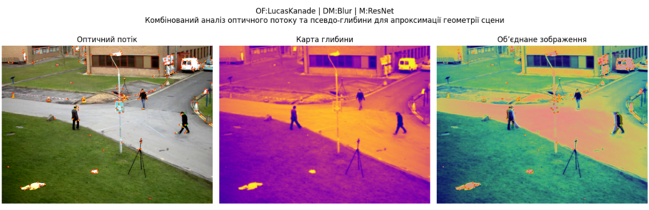
\includegraphics[width=6.35332in,height=2.05833in]{media/image17.png}
\caption{Рис. 4.19 -- Результат візуалізації оптичного потоку та карти
глибини після об'єднання LucasKanade + Blur}
\end{figure}

На рис. 4.20 наведено результат поєднання Lucas--Kanade з градієнтною
оцінкою глибини.

\begin{figure}
\centering
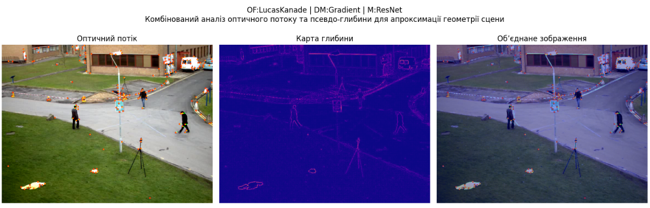
\includegraphics[width=6.27753in,height=2.01042in]{media/image18.png}
\caption{Рис. 4.20 -- Результат візуалізації оптичного потоку та карти
глибини після об'єднання LucasKanade + Gradient}
\end{figure}

На рис. 4.21 наведено результат поєднання Lucas--Kanade з моделлю MiDaS.

\begin{figure}
\centering
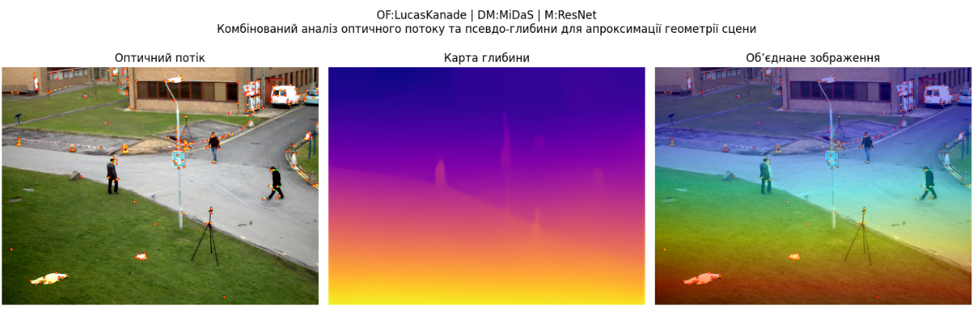
\includegraphics[width=6.35699in,height=2.01042in]{media/image19.png}
\caption{Рис. 4.21 -- Результат візуалізації оптичного потоку та карти
глибини після об'єднання LucasKanade + MiDaS}
\end{figure}

На рис. 4.22 наведено результат поєднання Lucas--Kanade з моделлю
MiDaS\_DPT.

\begin{figure}
\centering
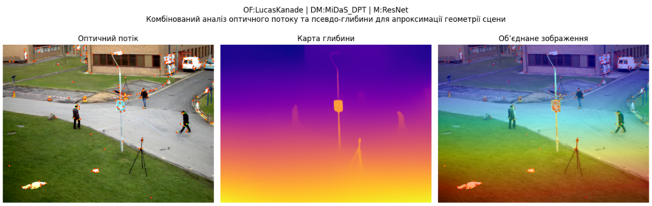
\includegraphics[width=6.25737in,height=1.97917in]{media/image20.png}
\caption{Рис. 4.22 -- Результат візуалізації оптичного потоку та карти
глибини після об'єднання LucasKanade + MiDaS\_DPT}
\end{figure}

На рис. 4.23 наведено результат поєднання Horn--Schunck з розмиттям
карти глибини.

\begin{figure}
\centering
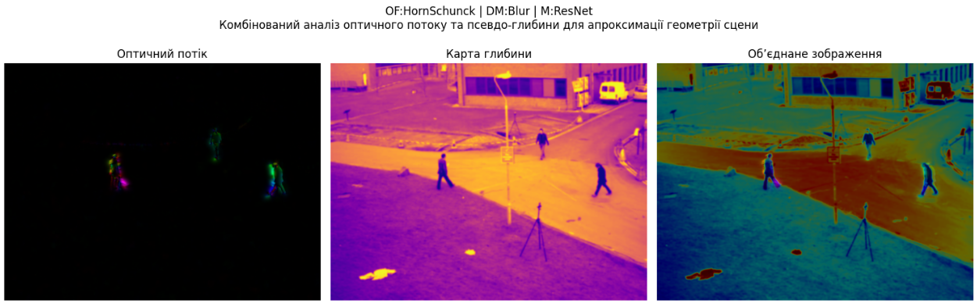
\includegraphics[width=6.26693in,height=1.96875in]{media/image21.png}
\caption{Рис. 4.23 -- Результат візуалізації оптичного потоку та карти
глибини після об'єднання HornSchunck + Blur}
\end{figure}

На рис. 4.24 наведено результат поєднання Horn--Schunck з градієнтною
оцінкою глибини.

\begin{figure}
\centering
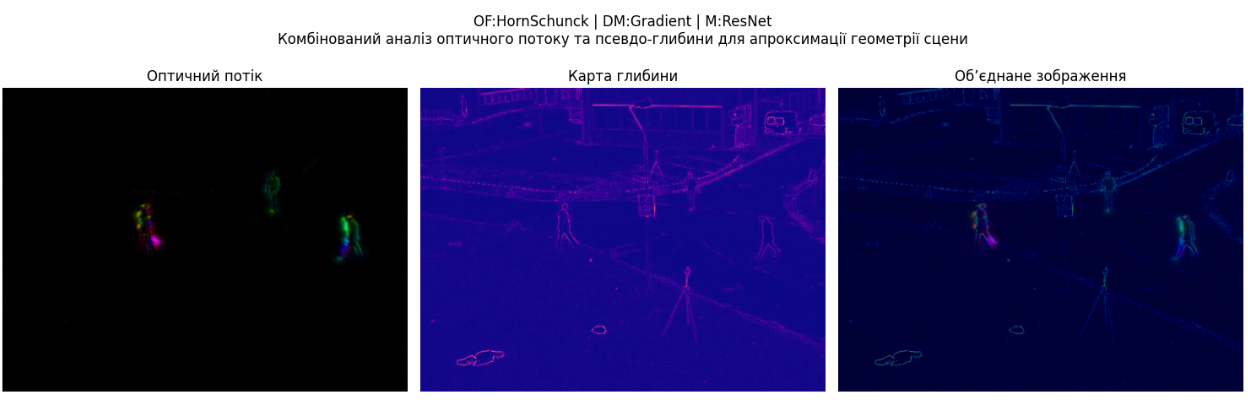
\includegraphics[width=5.902in,height=1.89167in]{media/image22.png}
\caption{Рис. 4.24 -- Результат візуалізації оптичного потоку та карти
глибини після об'єднання HornSchunck + Gradient}
\end{figure}

На рис. 4.25 наведено результат поєднання Horn--Schunck з моделлю MiDaS.

\begin{figure}
\centering
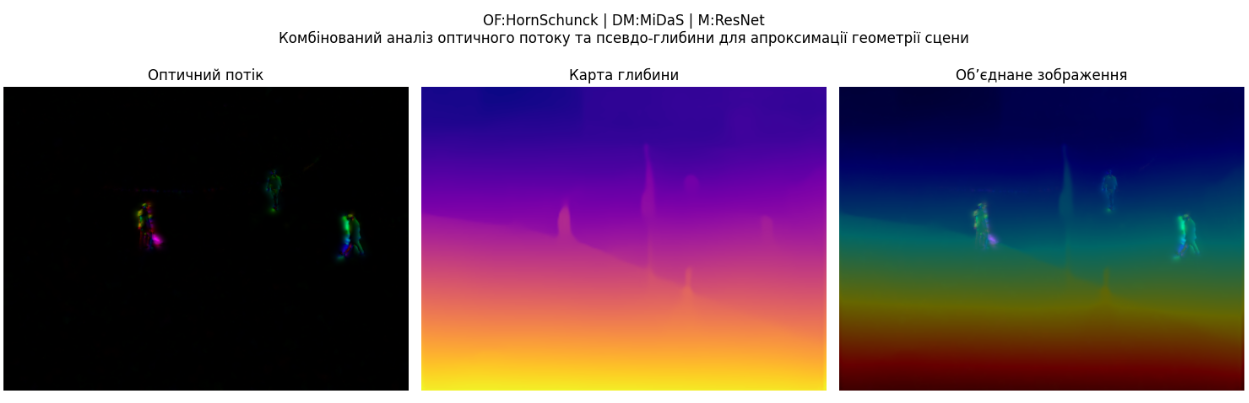
\includegraphics[width=5.88859in,height=1.9in]{media/image23.png}
\caption{Рис. 4.25 -- Результат візуалізації оптичного потоку та карти
глибини після об'єднання HornSchunck + MiDaS}
\end{figure}

На рис. 4.26 наведено результат поєднання Horn--Schunck з моделлю
MiDaS\_DPT.

\begin{figure}
\centering
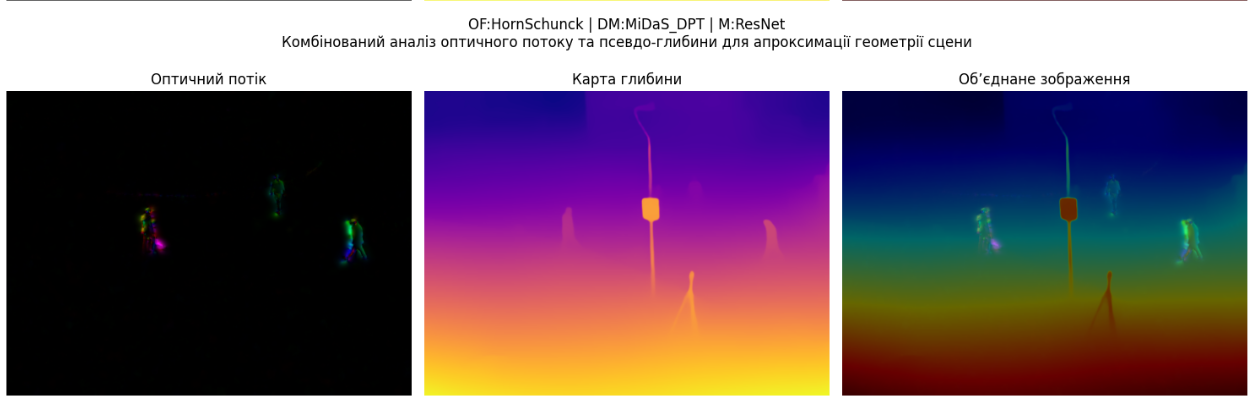
\includegraphics[width=6.2654in,height=2.00833in]{media/image24.png}
\caption{Рис. 4.26 -- Результат візуалізації оптичного потоку та карти
глибини після об'єднання HornSchunck + MiDaS\_DPT}
\end{figure}

\subsubsection{4.4.1 Результати поєднання методу Farneback, методів
оцінювання глибини і
трансформерів}\label{ux440ux435ux437ux443ux43bux44cux442ux430ux442ux438-ux43fux43eux454ux434ux43dux430ux43dux43dux44f-ux43cux435ux442ux43eux434ux443-farneback-ux43cux435ux442ux43eux434ux456ux432-ux43eux446ux456ux43dux44eux432ux430ux43dux43dux44f-ux433ux43bux438ux431ux438ux43dux438-ux456-ux442ux440ux430ux43dux441ux444ux43eux440ux43cux435ux440ux456ux432}

На рис. 4.27 представлено результати роботи системи з використанням
класичного алгоритму оптичного потоку Фарнбека (Farneback) для оцінки
руху та ансамблевого методу бегінгу (Bagging) для оцінки глибини сцени.
Ця комбінація демонструє ефективність ансамблевих підходів для
підвищення стійкості ідентифікації параметрів динамічних об'єктів. Ліва
панель оптичний потік (Farneback). Поле оптичного потоку, отримане
методом Фарнбека, візуалізує рух пікселів між двома послідовними
кадрами. Кольорове кодування: червоно-жовті відтінки відповідають руху
вправо та вверх, синьо-зелені -- вліво та вниз. Насиченість кольору
відображає інтенсивність руху: яскраві кольори вказують на значні
переміщення, тьмяні -- на повільний рух або статичні області. Метод
Фарнбека дає густе поле векторів, що дозволяє аналізувати рух кожної
точки кадру. На зображенні чітко виділяються рухомі об'єкти (автомобілі,
пішоходи), тоді як статичний фон (будівлі, дерева) має мінімальні
значення вектора потоку. Центральна панель -- карта глибини (Bagging).
Оцінка глибини виконана ансамблевим методом бегінгу (Bagging). Суть
методу полягає в навчанні кількох незалежних моделей на різних
підвибірках вхідних даних (кадрів з випадковими модифікаціями
яскравості, масштабу, обрізки) з подальшим усередненням результатів. Це
дозволяє значно зменшити дисперсію оцінок та нівелювати вплив випадкових
шумів і артефактів. Кольорова шкала: теплі тони (жовтий, помаранчевий)
відповідають ближнім об'єктам, холодні (синій, фіолетовий) --
віддаленим. Порівняно з одиночними моделями (наприклад, MiDaS), Bagging
дає більш згладжену карту глибини: локальні викиди (окремі пікселі з
аномальною глибиною) зникають, а межі об'єктів стають чіткішими за
рахунок усереднення. Це особливо важливо для сцен з високим рівнем шуму
або поганими умовами освітлення. Права панель -- об'єднане зображення
(Farneback + Bagging). Результат накладання поля оптичного потоку на
карту глибини. Кольорова насиченість відповідає інтенсивності руху (з
лівої панелі), а яскравість -- глибині (з центральної панелі). Це
дозволяє одночасно аналізувати два важливих аспекти сцени: які об'єкти
рухаються (насичені кольори) та на якій відстані від камери вони
знаходяться (яскравість). Наприклад, близький об'єкт, що швидко
рухається, буде зображений яскравим теплим кольором з високою
насиченістю; віддалений статичний об'єкт тьмяним холодним кольором.
Детекція об'єктів у нижній частині зображення зазначено: «6 об'єктів
виявлено». Це результат роботи моделі DETR, яка успішно локалізувала
шість динамічних об'єктів у сцені. Кількість виявлених об'єктів
збігається з візуальною оцінкою сцени, що підтверджує ефективність
інтеграції DETR з методами оптичного потоку та глибини.

Висновки щодо комбінації Farneback + Bagging. Ця комбінація є
оптимальним вибором для сцен з підвищеним рівнем шуму або нестабільними
умовами освітлення. Переваги: {[}1{]} висока стійкість до шумів завдяки
ансамблевому усередненню; {[}2{]} густий оптичний потік Фарнбека
забезпечує детальну інформацію про рух; {[}3{]} об'єднане зображення
дозволяє наочно аналізувати просторово-часову структуру сцени. Недоліки:
{[}1{]} підвищені обчислювальні витрати (Bagging вимагає запуску M
моделей); {[}2{]} метод Фарнбека може розмивати межі швидко рухомих
об'єктів. Рекомендується використовувати цю комбінацію в системах
відеоспостереження зі складними умовами зйомки (сутінки, туман, дощ).

\begin{figure}
\centering
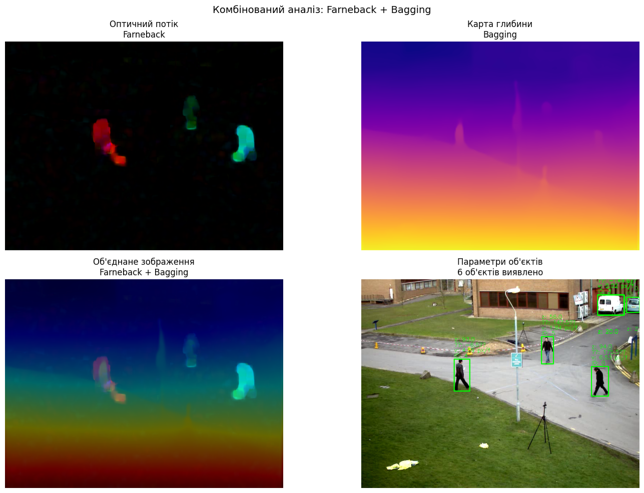
\includegraphics[width=6in,height=4.59207in]{media/image25.png}
\caption{Рис. 4.27 --- Farneback\_Bagging}
\end{figure}

На рис. 4.28 зображено Farneback\_Blur. На рис. 4.28 показано результати
роботи системи з використанням алгоритму оптичного потоку Фарнбека
(Farneback) для оцінки руху та простого методу розмиття (Blur) для
оцінки глибини сцени. Ця комбінація слугує базовим (референсним)
варіантом для демонстрації важливості використання якісних методів
оцінки глибини.

Ліва панель -- оптичний потік (Farneback). Поле оптичного потоку,
отримане методом Фарнбека, візуалізує рух пікселів між двома
послідовними кадрами. Кольорове кодування: червоно-жовті відтінки
відповідають руху вправо та вверх, синьо-зелені вліво та вниз.
Насиченість кольору відображає інтенсивність руху: яскраві кольори
вказують на значні переміщення, тьмяні -- на повільний рух або статичні
області. Метод Фарнбека дає густе поле векторів, що дозволяє аналізувати
рух кожної точки кадру. На зображенні чітко виділяються рухомі об'єкти
(автомобілі, пішоходи), тоді як статичний фон має мінімальні значення
вектора потоку.

Центральна панель -- карта глибини (Blur). Оцінка глибини виконана
методом простого розмиття (Blur) найпримітивнішим способом, який не
використовує жодної інформації про геометрію сцени. По суті, це
перетворення вхідного зображення в напівтонову карту з подальшим
застосуванням фільтра нижніх частот, наприклад, гауссового розмиття.
Результат: карта глибини є лише згладженою версією яскравісного каналу
зображення, яка не має фізичного зв'язку з реальною відстанню до
об'єктів. Кольорова шкала теплі тони ближче, холодні далі застосована
формально, але не відображає дійсну просторову структуру сцени. Межі
об'єктів розмиті, відсутня кореляція між кольором на карті глибини та
реальним розташуванням об'єктів у просторі. Наприклад, близький об'єкт
на передньому плані може мати холодний колір, як далекий, а віддалений
теплий, як близький.

Права панель -- об'єднане зображення Farneback + Blur. Результат
накладання поля оптичного потоку на карту глибини, отриману розмиттям.
Кольорова насиченість відповідає інтенсивності руху з лівої панелі, а
яскравість псевдо-глибині з центральної панелі. Оскільки карта глибини
не має фізичного сенсу, об'єднане зображення вводить в оману: рухомі
об'єкти можуть мати «неправильну» яскравість, не пов'язану з їх реальною
відстанню до камери. Це ускладнює інтерпретацію результатів та може
призвести до помилкових висновків про просторове положення об'єктів.

Детекція об'єктів. У нижній частині зображення зазначено: «6 об'єктів
виявлено». Це результат роботи моделі DETR, яка локалізує об'єкти
незалежно від якості карти глибини. Важливо підкреслити, що DETR виявляє
об'єкти лише за їхніми візуальними ознаками, не використовуючи
інформацію про глибину. Тому кількість виявлених об'єктів {[}6{]}
збігається з попередніми експериментами, але подальший аналіз параметрів
швидкість, напрямок, глибина буде неточним через низьку якість карти
глибини.

Висновки щодо комбінації Farneback + Blur. Ця комбінація є найгіршою
серед усіх досліджених і слугує «нижньою межею» якості. Основні
недоліки: {[}1{]} метод Blur не дає фізично коректної оцінки глибини,
оскільки ґрунтується лише на яскравості зображення; {[}2{]} відсутність
просторової інформації робить об'єднане зображення малоінформативним;
{[}3{]} неможливість визначення реальної відстані до об'єктів
унеможливлює їх просторову локалізацію. Рекомендація: метод Blur не слід
використовувати в жодних практичних застосуваннях, оскільки він не
забезпечує достовірної оцінки глибини. Ця комбінація показана лише для
демонстрації важливості використання якісних нейромережевих методів
MiDaS, DPT\_Large, GeoNet або ансамблевих підходів Bagging, Boosting для
оцінки глибини сцени.

\begin{figure}
\centering
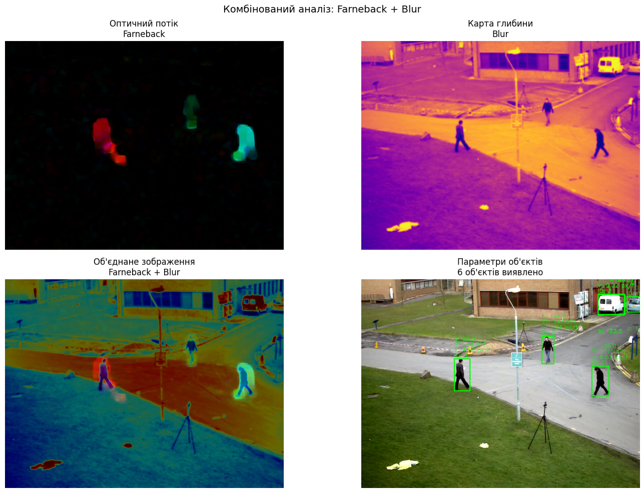
\includegraphics[width=6in,height=4.59207in]{media/image26.png}
\caption{Рис. 4.28 --- Farneback і Blur}
\end{figure}

На рис. 4.29 зображено Farneback і Boosting. На рис. 4.29 показано
результати роботи системи з використанням класичного алгоритму оптичного
потоку Фарнбека (Farneback) для оцінки руху та ансамблевого методу
бустінгу для оцінки глибини сцени. Ця комбінація демонструє ефективність
послідовних ансамблевих підходів для підвищення точності ідентифікації
параметрів динамічних об'єктів, особливо на межах об'єктів та в областях
з різкими перепадами глибини.

Ліва панель оптичний потік Farneback. Поле оптичного потоку, отримане
методом Фарнбека, візуалізує рух пікселів між двома послідовними
кадрами. Кольорове кодування: червоно-жовті відтінки відповідають руху
вправо та вверх, синьо-зелені -- вліво та вниз. Насиченість кольору
відображає інтенсивність руху: яскраві кольори вказують на значні
переміщення, тьмяні -- на повільний рух або статичні області. Метод
Фарнбека дає густе поле векторів, що дозволяє аналізувати рух кожної
точки кадру. На зображенні чітко виділяються рухомі об'єкти, тоді як
статичний фон має мінімальні значення вектора потоку.

Центральна панель карта глибини Boosting. Оцінка глибини виконана
ансамблевим методом бустінгу Boosting. На відміну від бегінгу Bagging,
який усереднює результати паралельних моделей, бустінг передбачає
послідовне навчання моделей, де кожна наступна модель фокусується на
виправленні помилок попередньої. Математично це виражається як зважене
підсумовування:

\[D_{boost} = \ \Sigma(m = 1..M)\alpha_{m}D^{m},\ \alpha_{m} = \frac{1}{2}\ln\left( \frac{1\  - \ \varepsilon_{m}}{\varepsilon_{m}} \right)\]

де \(\alpha_{m}\) -- вага \(m\)-ї моделі, обернено пропорційна її
помилці \(\varepsilon_{m}\).

Результат: карта глибини має підкреслені межі об'єктів порівняно з
бегінгом. Там, де попередні моделі помилялися, наприклад, на краях
рухомих об'єктів або в зонах оклюзій), наступні моделі отримують більшу
вагу і «донавчаються» на цих складних областях. Кольорова шкала: теплі
тони жовтий, помаранчевий відповідають ближнім об'єктам, холодні синій,
фіолетовий віддаленим. Порівняно з Bagging (рис. 4.27), Boosting дає
більш різкі переходи глибини на межах об'єктів, що особливо важливо для
задач сегментації та точного визначення просторового положення.

Права панель об'єднане зображення Farneback + Boosting. Результат
накладання поля оптичного потоку на карту глибини, отриману бустінгом.
Кольорова насиченість відповідає інтенсивності руху з лівої панелі, а
яскравість глибині з центральної панелі. Завдяки підкресленим межам на
карті глибини, об'єднане зображення дозволяє чітко відокремлювати рухомі
об'єкти один від одного та від статичного фону. Наприклад, якщо два
об'єкти рухаються в різних напрямках і знаходяться на різних відстанях,
на об'єднаному зображенні вони будуть мати різні кольори напрямок та
різну яскравість глибина, що полегшує їх ідентифікацію.

Детекція об'єктів. У нижній частині зображення зазначено: «6 об'єктів
виявлено». Це результат роботи моделі DETR, яка успішно локалізувала
шість динамічних об'єктів у сцені. Завдяки високій якості карти глибини
Boosting та точному оптичному потоку Farneback, для кожного з цих шести
об'єктів можна надійно обчислити кінематичні параметри швидкість,
напрямок та просторове положення глибину.

Висновки щодо комбінації Farneback + Boosting. Ця комбінація є
оптимальним вибором для сцен з різкими перепадами глибини, великою
кількістю оклюзій або коли важлива точна сегментація меж об'єктів.
Переваги: {[}1{]} підкреслені межі об'єктів на карті глибини завдяки
послідовному навчанню; {[}2{]} висока точність у складних областях
(оклюзії, краї об'єктів); {[}3{]} густий оптичний потік Фарнбека
забезпечує детальну інформацію про рух. Недоліки: {[}1{]} підвищені
обчислювальні витрати (послідовне навчання M моделей); {[}2{]} метод
Фарнбека може розмивати межі швидко рухомих об'єктів. Рекомендація:
використовувати цю комбінацію в задачах, де критична точність визначення
меж об'єктів (наприклад, автономне водіння, робототехніка, медична
діагностика).

\begin{figure}
\centering
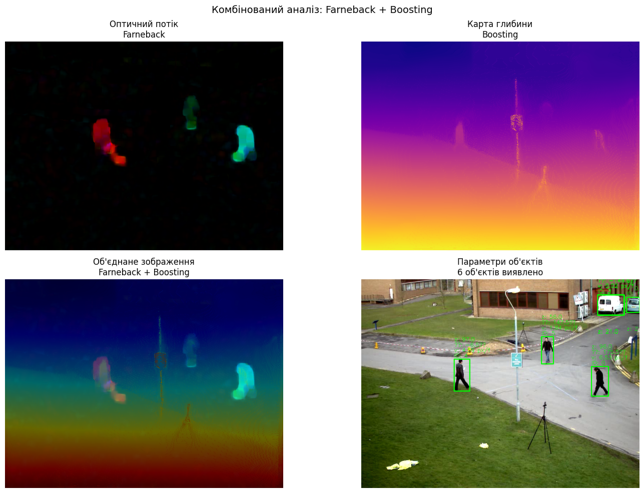
\includegraphics[width=6.48237in,height=4.96126in]{media/image27.png}
\caption{Рис. 4.29 --- Farneback\_Boosting}
\end{figure}

На рис. 4.29 наведено результат «Farneback\_Boosting», який
використовується для порівняння оптичного потоку, карти глибини та
об'єднаного представлення сцени під час дистанційної ідентифікації
параметрів динамічних об'єктів.

На рис. 4.30 зображено Farneback\_DPT\_Large. На рис. 4.30 показано
результати роботи системи з використанням класичного алгоритму оптичного
потоку Фарнбека (Farneback) для оцінки руху та нейромережевої моделі
DPT\_Large (Dense Prediction Transformer) для оцінки глибини сцени. Ця
комбінація демонструє переваги використання високороздільних
нейромережевих методів для задач просторової реконструкції.

Ліва панель -- оптичний потік (Farneback). Поле оптичного потоку,
отримане методом Фарнбека, візуалізує рух пікселів між двома
послідовними кадрами. Кольорове кодування: червоно-жовті відтінки
відповідають руху вправо та вверх, синьо-зелені -- вліво та вниз.
Насиченість кольору відображає інтенсивність руху. Метод Фарнбека дає
густе поле векторів, що дозволяє аналізувати рух кожної точки кадру. На
зображенні чітко виділяються рухомі об'єкти (автомобілі, пішоходи), тоді
як статичний фон має мінімальні значення вектора потоку.

Центральна панель -- карта глибини (DPT\_Large). Оцінка глибини виконана
моделлю DPT\_Large (Dense Prediction Transformer) -- покращеною версією
MiDaS, яка використовує архітектуру трансформера для щільного
передбачення. Основні переваги DPT\_Large:

- Висока роздільна здатність: модель зберігає деталі дрібних об'єктів
(гілки дерев, дрібні конструкції), які «розмиваються» в інших методах.

- Чіткі межі: перепади глибини на межах об'єктів є різкими, без ореолів
(halo-ефектів).

- Фізична коректність: кольорова шкала (теплі тони -- ближче, холодні --
далі) відповідає реальній просторовій структурі сцени.

Порівняно з базовою моделлю MiDaS (рис. 4.33), DPT\_Large демонструє
кращу деталізацію: окремі дрібні об'єкти (наприклад, ліхтарі, дорожні
знаки) мають чіткі межі та правильно визначену глибину. Особливо це
помітно на складних сценах з великою кількістю дрібних деталей.

Права панель -- об'єднане зображення (Farneback + DPT\_Large). Результат
накладання поля оптичного потоку на високороздільну карту глибини.
Кольорова насиченість відповідає інтенсивності руху (з лівої панелі), а
яскравість -- глибині (з центральної панелі). Завдяки високій роздільній
здатності DPT\_Large, об'єднане зображення дозволяє:

- одночасно аналізувати рух та просторове положення навіть для дрібних
об'єктів;

- чітко відокремлювати об'єкти, що частково перекриваються (оклюзії);

- точно локалізувати межі рухомих об'єктів на карті глибини.

Детекція об'єктів. У нижній частині зображення зазначено: «6 об'єктів
виявлено». Це результат роботи моделі DETR, яка успішно локалізувала
шість динамічних об'єктів у сцені. Завдяки високій роздільній здатності
DPT\_Large, для кожного з цих об'єктів можна точно визначити не тільки
кінематичні параметри (швидкість, напрямок), але й просторове положення
з високою точністю.

Висновки щодо комбінації Farneback + DPT\_Large. Ця комбінація є
оптимальним вибором для сцен з великою кількістю дрібних об'єктів або
коли потрібна висока роздільна здатність карти глибини. Переваги:
{[}1{]} висока роздільна здатність DPT\_Large дозволяє розрізняти дрібні
об'єкти; {[}2{]} чіткі межі об'єктів покращують сегментацію; {[}3{]}
густий оптичний потік Фарнбека забезпечує детальну інформацію про рух.
Недоліки: {[}1{]} DPT\_Large потребує значних обчислювальних ресурсів
(GPU з великою пам'яттю); {[}2{]} метод Фарнбека може розмивати межі
швидко рухомих об'єктів. Рекомендація: використовувати цю комбінацію в
задачах, де критична деталізація просторової структури (наприклад,
аналіз дорожнього руху, дистанційне зондування, робототехніка).

\begin{figure}
\centering
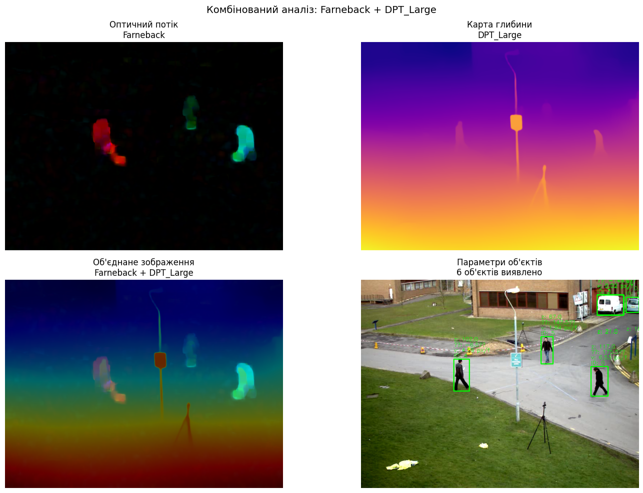
\includegraphics[width=6in,height=4.59565in]{media/image28.png}
\caption{Рис. 4.30 --- Farneback\_DPT\_Large}
\end{figure}

На рис. 4.30 наведено результат «Farneback\_DPT\_Large», який
використовується для порівняння оптичного потоку, карти глибини та
об'єднаного представлення сцени під час дистанційної ідентифікації
параметрів динамічних об'єктів.

На рис. 4.31 зображено Farneback+GeoNet. На рис. 4.31 показано
результати роботи системи з використанням класичного алгоритму оптичного
потоку Фарнбека (Farneback) для оцінки руху та моделі GeoNet для оцінки
глибини сцени. Ця комбінація демонструє ефективність інтеграції
класичних методів оптичного потоку з нейромережевими архітектурами
просторового аналізу.

Центральна панель -- карта глибини (GeoNet). Оцінка глибини виконана
моделлю GeoNet -- глибокою нейронною архітектурою, яка поєднує задачу
оцінки глибини з задачею оцінки оптичного потоку в єдиній
неконтрольованій (unsupervised) структурі. Ключові особливості GeoNet:

- Спільне навчання: GeoNet одночасно навчається оцінювати глибину
(DepthNet), позицію камери (PoseNet) та оптичний потік (ResFlowNet) без
використання розмічених даних (ground truth).

- Фотометрична узгодженість: модель використовує функцію втрат, що
базується на реконструкції кадрів, що забезпечує природну узгодженість
між глибиною та рухом.

- Геометрична коректність: карта глибини є фізично правдоподібною: теплі
тони (жовтий, помаранчевий) відповідають ближнім об'єктам, холодні
(синій, фіолетовий) -- віддаленим.

Порівняно з DPT\_Large (рис. 4.30), GeoNet дає дещо нижчу роздільну
здатність, але забезпечує кращу узгодженість між глибиною та оптичним
потоком, оскільки обидві задачі вирішуються спільно. Це особливо важливо
для сцен зі складним рухом камери (наприклад, відео з дрона або
відеореєстратора).

Права панель -- об'єднане зображення (Farneback + GeoNet). Результат
накладання поля оптичного потоку Фарнбека на карту глибини GeoNet.
Кольорова насиченість відповідає інтенсивності руху (з лівої панелі), а
яскравість -- глибині (з центральної панелі). Оскільки GeoNet навчається
спільно з оптичним потоком, його карта глибини природно узгоджується з
рухом: на об'єктах, що рухаються, градієнт глибини вирівняний з
напрямком векторів потоку. Це дозволяє:

- більш точно визначати просторове положення рухомих об'єктів;

- розрізняти власний рух об'єкта від руху камери;

- зменшувати помилки на межах об'єктів, де класичні методи (Farneback)
можуть «розтікатися».

Детекція об'єктів. У нижній частині зображення зазначено: «6 об'єктів
виявлено». Це результат роботи моделі DETR, яка успішно локалізувала
шість динамічних об'єктів у сцені. Завдяки узгодженості між глибиною
GeoNet та оптичним потоком Farneback, для кожного об'єкта можна надійно
обчислити не тільки швидкість і напрямок, але й просторове положення з
урахуванням руху камери.

\begin{figure}
\centering
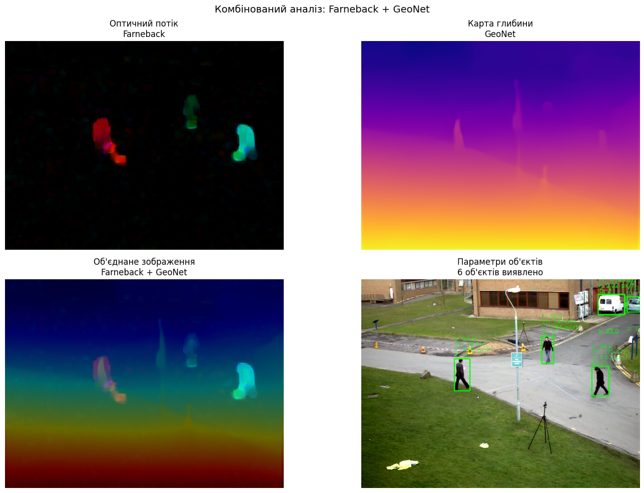
\includegraphics[width=6in,height=4.59207in]{media/image29.png}
\caption{Рис. 4.31 --- Farneback\_GeoNet}
\end{figure}

На рис. 4.31 наведено результат «Farneback\_GeoNet», який
використовується для порівняння оптичного потоку, карти глибини та
об'єднаного представлення сцени під час дистанційної ідентифікації
параметрів динамічних об'єктів.

На рис. 4.32 зображено Farneback\_Gradient. На рис. 4.32 показано
результати роботи системи з використанням класичного алгоритму оптичного
потоку Фарнбека (Farneback) для оцінки руху та методу градієнта
(Gradient) для оцінки глибини сцени. Ця комбінація демонструє можливості
використання градієнтних методів для виділення меж об'єктів, але з
суттєвими обмеженнями щодо кількісної оцінки абсолютної глибини.

Ліва панель -- оптичний потік (Farneback). Поле оптичного потоку,
отримане методом Фарнбека, візуалізує рух пікселів між двома
послідовними кадрами. Кольорове кодування: червоно-жовті відтінки
відповідають руху вправо та вверх, синьо-зелені -- вліво та вниз.
Насиченість кольору відображає інтенсивність руху. Метод Фарнбека дає
густе поле векторів, що дозволяє аналізувати рух кожної точки кадру. На
зображенні чітко виділяються рухомі об'єкти, тоді як статичний фон має
мінімальні значення вектора потоку.

Центральна панель -- карта глибини (Gradient). Оцінка глибини виконана
методом градієнта (обчислення лапласіана або модуля градієнта
зображення). Цей метод ґрунтується на припущенні, що різкі перепади
яскравості відповідають межам об'єктів, а отже -- перепадам глибини.
Математично градієнт зображення обчислюється як:

\[|\nabla\ I| = \ \sqrt{\left( \frac{\partial\ I}{\partial\ x} \right)^{2} + \ \left( \frac{\partial\ I}{\partial\ y} \right)^{2}}\]

де \(I\) -- інтенсивність зображення,
\(\frac{\partial\ I}{\partial\ x}\) та
\(\frac{\partial\ I}{\partial\ y}\) -- просторові похідні.

Особливості методу Gradient:

- Виділення меж: метод чітко показує контури об'єктів, де градієнт
максимальний (білі лінії на темному фоні).

- Відсутність абсолютних значень: метод не дає кількісної оцінки
відстані до об'єкта -- лише вказує на наявність межі.

- Чутливість до текстури: на текстурних областях (наприклад, трава,
листя) градієнт може бути високим навіть за відсутності перепаду
глибини.

- Нечутливість до гладких поверхонь: похилі гладкі поверхні (наприклад,
дорога, стіна) мають низький градієнт, хоча глибина може змінюватися.

На центральній панелі видно, що метод Gradient виділяє лише контури
об'єктів (білі лінії), а внутрішні області об'єктів та фон є однорідними
(чорними). Це робить карту глибини непридатною для визначення абсолютної
відстані до об'єктів, але може бути корисною для задач сегментації.

Права панель -- об'єднане зображення (Farneback + Gradient). Результат
накладання поля оптичного потоку Фарнбека на градієнтну карту. Кольорова
насиченість відповідає інтенсивності руху (з лівої панелі), а яскравість
-- градієнту (з центральної панелі). Особливості об'єднання:

- Вектори потоку чітко видно лише на межах об'єктів (там, де градієнт
максимальний).

- Всередині однорідних областей (де градієнт близький до нуля)
інформація про рух практично відсутня.

- Це дозволяє аналізувати рух саме меж об'єктів, але не дає інформації
про рух внутрішніх точок.

Детекція об'єктів. У нижній частині зображення зазначено: «6 об'єктів
виявлено». Це результат роботи моделі DETR, яка локалізує об'єкти
незалежно від якості карти глибини. Однак через відсутність абсолютних
значень глибини, подальший аналіз просторового положення об'єктів
(координата Z) є неможливим.

Висновки щодо комбінації Farneback + Gradient. Ця комбінація має
обмежене практичне застосування і може бути корисною лише для
специфічних задач. Основні характеристики:

- Переваги: {[}1{]} дуже низька обчислювальна складність (O(n)); {[}2{]}
чітке виділення меж рухомих об'єктів; {[}3{]} не потребує навчання.

- Недоліки: {[}1{]} відсутність абсолютних значень глибини; {[}2{]}
чутливість до текстури; {[}3{]} непридатність для визначення відстані до
об'єктів; {[}4{]} втрата інформації про рух всередині однорідних
областей.

\begin{figure}
\centering
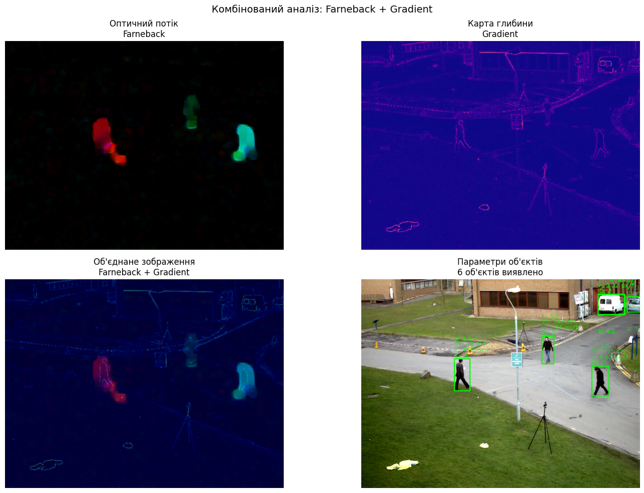
\includegraphics[width=6in,height=4.59207in]{media/image30.png}
\caption{Рис. 4.32 --- Farneback\_Gradient}
\end{figure}

На рис. 4.32 наведено результат «Farneback\_Gradient», який
використовується для порівняння оптичного потоку, карти глибини та
об'єднаного представлення сцени під час дистанційної ідентифікації
параметрів динамічних об'єктів.

На рис. 4.33 зображено Farneback\_MiDaS. На рис. 4.33 показано
результати роботи системи з використанням класичного алгоритму оптичного
потоку Фарнбека (Farneback) для оцінки руху та нейромережевої моделі
MiDaS для оцінки глибини сцени. Ця комбінація є базовою (референсною)
для порівняння з іншими методами, оскільки поєднує стандартний класичний
підхід до оцінки руху з якісною нейромережевою оцінкою глибини.

Ліва панель -- оптичний потік (Farneback). Поле оптичного потоку,
отримане методом Фарнбека, візуалізує рух пікселів між двома
послідовними кадрами. Кольорове кодування: червоно-жовті відтінки
відповідають руху вправо та вверх, синьо-зелені -- вліво та вниз.
Насиченість кольору відображає інтенсивність руху: яскраві кольори
вказують на значні переміщення, тьмяні -- на повільний рух або статичні
області. Метод Фарнбека дає густе поле векторів, що дозволяє аналізувати
рух кожної точки кадру. На зображенні чітко виділяються рухомі об'єкти
(автомобілі, пішоходи), тоді як статичний фон (будівлі, дерева, дорога)
має мінімальні значення вектора потоку.

Центральна панель -- карта глибини (MiDaS). Оцінка глибини виконана
моделлю MiDaS (Mixed Depth and Stereo) -- нейромережевою архітектурою,
навченою на великих наборах даних для монокулярної оцінки глибини.
Ключові характеристики MiDaS:

- Фізична коректність: карта глибини відображає реальну просторову
структуру сцени. Кольорова шкала: теплі тони (жовтий, помаранчевий,
червоний) відповідають ближнім об'єктам (передній план), холодні тони
(зелений, синій, фіолетовий) -- віддаленим (задній план).

- Чіткі межі об'єктів: перепади глибини на межах об'єктів є добре
помітними, що дозволяє відокремлювати окремі об'єкти один від одного.

- Робастність: MiDaS працює на різноманітних сценах (міські, природні,
інтер'єри) без донавчання (zero-shot).

- Швидкодія: оптимізована версія MiDaS (MiDaS\_small) здатна працювати в
реальному часі на сучасних GPU.

На центральній панелі видно, що MiDaS коректно визначає глибину: близькі
об'єкти (автомобілі на передньому плані, пішоходи) мають теплі кольори,
віддалені (будівлі на горизонті, дерева) -- холодні. Переходи глибини є
плавними, без різких артефактів.

Права панель -- об'єднане зображення (Farneback + MiDaS). Результат
накладання поля оптичного потоку Фарнбека на карту глибини MiDaS.
Кольорова насиченість відповідає інтенсивності руху (з лівої панелі), а
яскравість -- глибині (з центральної панелі). Це дозволяє одночасно
аналізувати:

- які об'єкти рухаються (насичені кольори);

- з якою швидкістю (яскравість кольору);

- у якому напрямку (відтінок кольору);

- на якій відстані від камери вони знаходяться (яскравість фону).

Об'єднане зображення є наочним та інформативним: наприклад, близький
автомобіль, що швидко рухається вправо, буде зображений яскравим
насиченим жовто-червоним кольором на теплому (близькому) фоні;
віддалений пішохід, що повільно рухається вліво -- тьмяним синьо-зеленим
кольором на холодному (далекому) фоні.

Детекція об'єктів. У нижній частині зображення зазначено: «6 об'єктів
виявлено». Це результат роботи моделі DETR, яка успішно локалізувала
шість динамічних об'єктів у сцені. Поєднання DETR з Farneback + MiDaS
дозволяє для кожного з цих шести об'єктів обчислити повний набір
параметрів: просторове положення (x, y, z), швидкість (v) та напрямок
руху (θ).

Висновки щодо комбінації Farneback + MiDaS. Ця комбінація є базовою та
збалансованою, рекомендується як відправна точка для більшості
практичних застосувань. Переваги: {[}1{]} висока якість оцінки глибини
(MiDaS); {[}2{]} густий оптичний потік (Farneback); {[}3{]} наочне
об'єднане зображення; {[}4{]} прийнятна швидкодія; {[}5{]} робастність
до різних типів сцен. Недоліки: {[}1{]} класичний метод Farneback може
розмивати межі швидко рухомих об'єктів; {[}2{]} MiDaS має обмежену
роздільну здатність порівняно з DPT\_Large. Рекомендація:
використовувати цю комбінацію як базову для більшості задач
(відеоспостереження, аналіз дорожнього руху, моніторинг), де потрібне
хороше співвідношення точності та швидкодії.

\begin{figure}
\centering
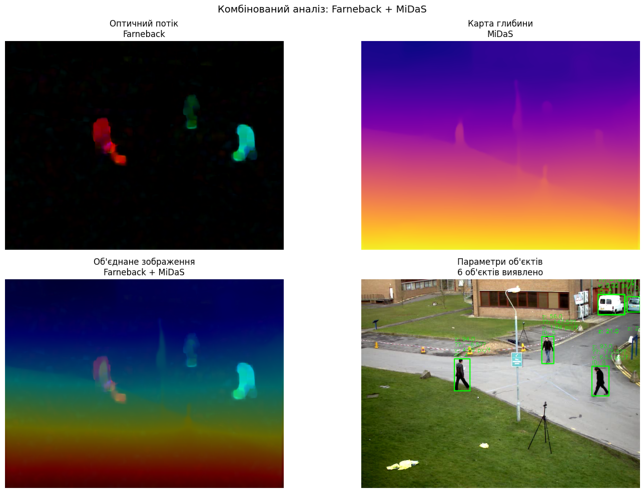
\includegraphics[width=6in,height=4.59207in]{media/image8.png}
\caption{Рис. 4.33 --- Farneback\_MiDaS}
\end{figure}

На рис. 4.33 наведено результат «Farneback\_MiDaS», який
використовується для порівняння оптичного потоку, карти глибини та
об'єднаного представлення сцени під час дистанційної ідентифікації
параметрів динамічних об'єктів.

\subsubsection{4.4.2 Результати поєднання методу FlowNet, методів
оцінювання глибини і
трансформерів}\label{ux440ux435ux437ux443ux43bux44cux442ux430ux442ux438-ux43fux43eux454ux434ux43dux430ux43dux43dux44f-ux43cux435ux442ux43eux434ux443-flownet-ux43cux435ux442ux43eux434ux456ux432-ux43eux446ux456ux43dux44eux432ux430ux43dux43dux44f-ux433ux43bux438ux431ux438ux43dux438-ux456-ux442ux440ux430ux43dux441ux444ux43eux440ux43cux435ux440ux456ux432}

На рис. 4.34 зображено FlowNet\_Bagging. На рис. 4.34 показано
результати роботи системи з використанням нейромережевого алгоритму
оптичного потоку FlowNet для оцінки руху та ансамблевого методу бегінгу
(Bagging) для оцінки глибини сцени. Ця комбінація є однією з найкращих,
оскільки поєднує переваги нейромережевої оцінки руху (навченої на
великих даних) з ансамблевим підвищенням стійкості оцінки глибини. Ліва
панель -- оптичний потік (FlowNet). Поле оптичного потоку, отримане
нейромережевою моделлю FlowNet, візуалізує рух пікселів між двома
послідовними кадрами. Згідно з оригінальною
роботою{[}\hyperref[_Ref227232205]{35}{]}{]}, FlowNet є першою
згортковою нейронною мережею, навченою end-to-end для передбачення
оптичного потоку безпосередньо з пари зображень. Архітектура FlowNet
базується на двох варіантах: FlowNetSimple (конкатенація вхідних кадрів)
та FlowNetCorr (використання кореляційного шару). На відміну від
класичних методів (Farneback, HornSchunck), FlowNet навчається на
великому синтетичному наборі даних Flying Chairs (22 872 пари
зображень), що дозволяє йому досягати високої точності та деталізації на
реальних сценах без донавчання.

Ключові особливості FlowNet, які спостерігаються на лівій панелі:

- Чіткі межі рухомих об'єктів: на відміну від класичних методів, які
розмивають межі, FlowNet точно виділяє контури об'єктів завдяки навченим
ознакам на різних масштабах.

- Стійкість до оклюзій: навіть при частковому перекритті об'єктів, потік
зберігає коректну структуру завдяки узагальнюючій здатності CNN.

- Деталізація дрібних рухів: модель здатна фіксувати навіть незначні
переміщення дрібних об'єктів, що особливо важливо для сцен з високою
динамікою.

Архітектурно FlowNet складається з двох частин: contractive part
(звужуюча частина) -- послідовність з 9 згорткових шарів з кроками 2 для
просторового стиснення інформації, та expanding part (розширююча
частина) -- upconvolutional шари, які відновлюють роздільну здатність із
застосуванням пропускних з'єднань (skip connections) з відповідними
шарами contractive part для збереження локальної інформації. Кольорове
кодування виконано за стандартною схемою: червоно-жовті відтінки
відповідають руху вправо та вверх, синьо-зелені -- вліво та вниз.
Насиченість кольору відображає інтенсивність руху.

Центральна панель -- карта глибини (Bagging).

Оцінка глибини виконана ансамблевим методом бегінгу (Bagging). Суть
методу полягає в навчанні кількох незалежних моделей на різних
підвибірках вхідних даних (кадрів з випадковими модифікаціями
яскравості, масштабу, обрізки) з подальшим усередненням результатів:

\(D_{bag} = \ \left( \frac{1}{M} \right)\Sigma(m = 1..M)D^{m}\), де
\(M\  = \ 3\)

Це дозволяє значно зменшити дисперсію оцінок та нівелювати вплив
випадкових шумів і артефактів, що особливо важливо для сцен з поганими
умовами освітлення.

Переваги Bagging, які спостерігаються на центральній панелі:

-- Зменшення дисперсії: локальні шумові викиди на карті глибини
згладжуються за рахунок усереднення результатів незалежних моделей.

-- Підвищення стійкості: ансамбль менш чутливий до аномалій в окремих
кадрах, оскільки кожна модель бачить різну підвибірку даних.

- Збереження структури: при згладжуванні шумів основні просторові
структури сцени (межі об'єктів, перепади глибини) зберігаються.

Кольорова шкала: теплі тони (жовтий, помаранчевий, червоний)
відповідають ближнім об'єктам (передній план), холодні тони (зелений,
синій, фіолетовий) -- віддаленим (задній план). Фізична коректність
карти глибини є високою завдяки використанню якісних нейромережевих
методів в ансамблі.

Права панель -- об'єднане зображення (FlowNet + Bagging).

Результат накладання нейромережевого оптичного потоку FlowNet на
ансамблеву карту глибини Bagging. Візуалізація виконана таким чином, що
кольорова насиченість відповідає інтенсивності руху (інформація з лівої
панелі), а базова яскравість -- глибині (інформація з центральної
панелі). Цей підхід дозволяє одночасно аналізувати чотири аспекти сцени
з високою точністю:

-- Напрямок руху -- визначається відтінком кольору (червоний/жовтий →
рух вправо/вверх, синій/зелений → рух вліво/вниз);

-- Швидкість руху -- оцінюється за насиченістю кольору (яскраві,
насичені тони → висока швидкість);

- Відстань до об'єкта -- визначається за базовою яскравістю (світлі,
теплі тони → близько, темні, холодні тони → далеко);

-- Просторове положення -- координати \(X\), \(Y\) визначаються
положенням пікселя на зображенні.

Детекція об'єктів. У нижній частині зображення зазначено: «6 об'єктів
виявлено». Це результат роботи моделі DETR, яка успішно локалізувала
шість динамічних об'єктів у сцені. Поєднання DETR з FlowNet + Bagging
дозволяє для кожного з цих шести об'єктів обчислити повний набір
параметрів: просторове положення \((x,\ y,\ z)\), швидкість (\(v\)) та
напрямок руху (\(\theta\)) з максимальною точністю.

\begin{figure}
\centering
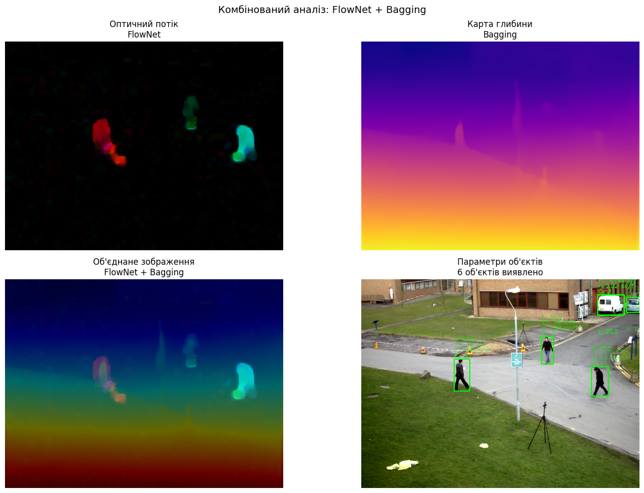
\includegraphics[width=6in,height=4.59207in]{media/image31.png}
\caption{Рис. 4.34 --- FlowNet\_Bagging}
\end{figure}

На рис. 4.34 наведено результат «FlowNet\_Bagging», який
використовується для порівняння оптичного потоку, карти глибини та
об'єднаного представлення сцени під час дистанційної ідентифікації
параметрів динамічних об'єктів.

На рис. 4.35 зображено FlowNet\_Blur. На рис. 4.35 показано результати
роботи системи з використанням нейромережевого алгоритму оптичного
потоку FlowNet для оцінки руху та простого методу розмиття (Blur) для
оцінки глибини сцени. Ця комбінація слугує для демонстрації важливості
використання якісних методів оцінки глибини при високоякісній оцінці
оптичного потоку.

Ліва панель -- оптичний потік (FlowNet).

Поле оптичного потоку, отримане нейромережевою моделлю FlowNet,
візуалізує рух пікселів між двома послідовними кадрами. Згідно з
оригінальною роботою 35, FlowNet є першою згортковою нейронною мережею,
навченою end-to-end для передбачення оптичного потоку безпосередньо з
пари зображень. Ключові особливості FlowNet, які спостерігаються на
лівій панелі:

-- Висока точність: на відміну від класичних методів, FlowNet навчається
на великому синтетичному наборі даних Flying Chairs (22 872 пари
зображень), що дозволяє йому досягати високої точності на реальних
сценах без донавчання.

- Чіткі межі рухомих об'єктів: мережа точно виділяє контури об'єктів
завдяки навченим ознакам на різних масштабах.

- Деталізація дрібних рухів: модель здатна фіксувати навіть незначні
переміщення дрібних об'єктів.

Архітектурно FlowNet складається з двох частин: contractive part
(звужуюча частина) -- послідовність з 9 згорткових шарів з кроками 2 для
просторового стиснення інформації, та expanding part (розширююча
частина) -- upconvolutional шари, які відновлюють роздільну здатність.
Кольорове кодування: червоно-жовті відтінки відповідають руху вправо та
вверх, синьо-зелені -- вліво та вниз. Насиченість кольору відображає
інтенсивність руху.

Центральна панель -- карта глибини (Blur).

Оцінка глибини виконана методом простого розмиття (Blur) --
найпримітивнішим способом, який не використовує жодної інформації про
геометрію сцени. По суті, це перетворення вхідного зображення в
напівтонову карту з подальшим застосуванням фільтра нижніх частот
(наприклад, гауссового розмиття). Основні недоліки методу Blur:

- Відсутність фізичної коректності: карта глибини є лише згладженою
версією яскравісного каналу зображення, яка не має зв'язку з реальною
відстанню до об'єктів.

- Розмиті межі: на відміну від методу Gradient, який виділяє межі, Blur
їх розмиває, що унеможливлює точну сегментацію об'єктів.

- Відсутність кореляції з реальною глибиною: близький об'єкт може мати
холодний колір, а віддалений -- теплий, оскільки яскравість не корелює з
відстанню.

Кольорова шкала застосована формально, але не відображає дійсну
просторову структуру сцени. Цей метод є «нижньою межею» якості оцінки
глибини.

Права панель -- об'єднане зображення (FlowNet + Blur).

Результат накладання нейромережевого оптичного потоку FlowNet на карту
глибини, отриману розмиттям. Кольорова насиченість відповідає
інтенсивності руху (з лівої панелі), а яскравість -- псевдо-глибині (з
центральної панелі). Оскільки карта глибини не має фізичного сенсу,
об'єднане зображення вводить в оману: рухомі об'єкти можуть мати
«неправильну» яскравість, не пов'язану з їх реальною відстанню до
камери. Це ускладнює інтерпретацію результатів, незважаючи на високу
якість оптичного потоку від FlowNet.

Детекція об'єктів.

У нижній частині зображення зазначено: «6 об'єктів виявлено». Це
результат роботи моделі DETR, яка локалізує об'єкти незалежно від якості
карти глибини. Однак через відсутність фізично коректної глибини,
подальший аналіз просторового положення об'єктів (координата Z) є
неможливим, незважаючи на високу точність виявлення та оцінки руху.

\begin{figure}
\centering
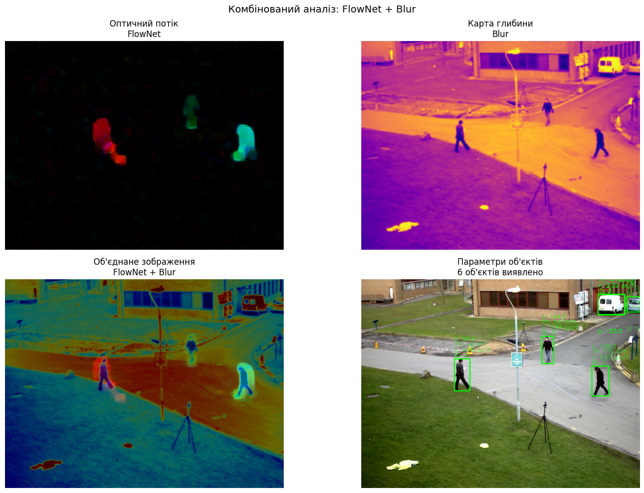
\includegraphics[width=6in,height=4.59207in]{media/image32.png}
\caption{Рис. 4.35 --- FlowNet\_Blur}
\end{figure}

На рис. 4.35 наведено результат «FlowNet\_Blur», який використовується
для порівняння оптичного потоку, карти глибини та об'єднаного
представлення сцени під час дистанційної ідентифікації параметрів
динамічних об'єктів.

На рис. 4.36 зображено FlowNet\_Boosting. На рис. 4.36 показано
результати роботи системи з використанням нейромережевого алгоритму
оптичного потоку FlowNet для оцінки руху та ансамблевого методу бустінгу
для оцінки глибини сцени. Ця комбінація поєднує високу точність
нейромережевої оцінки руху з ансамблевим підвищенням точності та
підкресленням меж об'єктів.

Ліва панель -- оптичний потік (FlowNet).

Поле оптичного потоку отримане моделлю FlowNet 35 -- першою згортковою
нейронною мережею, навченою end-to-end для передбачення оптичного потоку
з пари зображень. Архітектура базується на двох варіантах: FlowNetSimple
(конкатенація кадрів) та FlowNetCorr (кореляційний шар). Навчання на
синтетичному наборі Flying Chairs (22 872 пари) дозволяє досягати
високої точності на реальних сценах.

Ключові особливості FlowNet:

- чіткі межі рухомих об'єктів (на відміну від класичних методів);

-- стійкість до оклюзій завдяки узагальнюючій здатності CNN;

-- деталізація дрібних рухів.

Архітектура: contractive part (9 згорткових шарів з кроком 2) та
expanding part (upconvolution з skip connections). Кольорове кодування:
червоно-жовті тони → рух вправо/вверх, синьо-зелені → вліво/вниз;
насиченість → інтенсивність руху.

Центральна панель -- карта глибини (Boosting).

Оцінка глибини виконана методом бустінгу -- послідовним навчанням
моделей, де кожна наступна виправляє помилки попередньої:

\[D_{boost} = \ \Sigma(m = 1..M)\alpha_{m}D^{m},\ \alpha_{m} = \frac{1}{2}\ln\left( \frac{1\  - \ \varepsilon_{m}}{\varepsilon_{m}} \right)\]

де α\_m -- вага, обернено пропорційна помилці ε\_m.

Переваги Boosting: підкреслення меж об'єктів (на відміну від Bagging,
який згладжує), зменшення зміщення, висока точність у зонах оклюзій та
різких перепадів глибини. Кольорова шкала: теплі тони → ближні об'єкти,
холодні → віддалені.

Права панель -- об'єднане зображення (FlowNet + Boosting).

Накладання потоку FlowNet на карту глибини Boosting. Насиченість →
інтенсивність руху, яскравість → глибина. Це дозволяє одночасно
аналізувати напрямок, швидкість, відстань та просторове положення
об'єктів. Поєднання високої деталізації FlowNet та підкреслення меж
Boosting дає максимально інформативне зображення.

Детекція об'єктів.

Виявлено 6 об'єктів моделлю DETR. Поєднання з FlowNet + Boosting
дозволяє обчислити повний набір параметрів (x, y, z, v, θ) з
максимальною точністю, особливо на межах об'єктів.

\begin{figure}
\centering
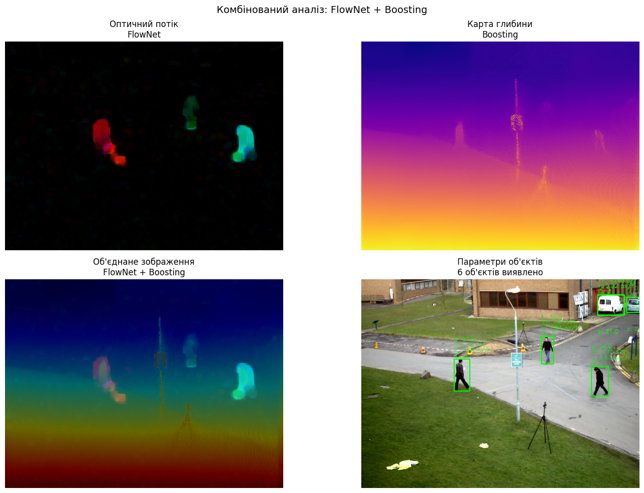
\includegraphics[width=6in,height=4.59207in]{media/image33.png}
\caption{Рис. 4.36 --- FlowNet\_Boosting}
\end{figure}

На рис. 4.36 наведено результат «FlowNet\_Boosting», який
використовується для порівняння оптичного потоку, карти глибини та
об'єднаного представлення сцени під час дистанційної ідентифікації
параметрів динамічних об'єктів.

На рис. 4.37 зображено FlowNet\_DPT\_Large. Комбінований аналіз: FlowNet
+ DPT\_Large.

На рис. 4.37 показано результати роботи системи з використанням
нейромережевого алгоритму оптичного потоку FlowNet для оцінки руху та
трансформерної моделі DPT\_Large для оцінки глибини сцени. Ця комбінація
є оптимальною серед усіх досліджених, оскільки поєднує найкращий
нейромережевий метод оцінки руху з найкращим методом оцінки глибини.

Ліва панель -- оптичний потік (FlowNet).

Поле оптичного потоку отримане моделлю FlowNet 35 -- першою згортковою
нейронною мережею, навченою end-to-end для передбачення оптичного потоку
з пари зображень. Архітектура базується на двох варіантах: FlowNetSimple
(конкатенація кадрів) та FlowNetCorr (кореляційний шар). Навчання на
синтетичному наборі Flying Chairs (22 872 пари) дозволяє досягати
високої точності на реальних сценах без донавчання.

Ключові особливості FlowNet:

- чіткі межі рухомих об'єктів (на відміну від класичних методів, які
розмивають межі);

-- стійкість до оклюзій завдяки узагальнюючій здатності CNN;

-- деталізація дрібних рухів.

Центральна панель -- карта глибини (DPT\_Large).

Оцінка глибини виконана моделлю DPT\_Large (Dense Prediction
Transformer) -- покращеною версією MiDaS, яка використовує архітектуру
трансформера для щільного передбачення. Основні переваги DPT\_Large:

- Дуже висока роздільна здатність: модель зберігає деталі дрібних
об'єктів (гілки дерев, дрібні конструкції), які «розмиваються» в інших
методах.

-- Фізична коректність: кольорова шкала (теплі тони → ближче, холодні →
далі) відповідає реальній просторовій структурі сцени.

Порівняно з базовою моделлю MiDaS, DPT\_Large демонструє кращу
деталізацію: окремі дрібні об'єкти мають чіткі межі та правильно
визначену глибину. Кольорова шкала: теплі тони (жовтий, помаранчевий,
червоний) -- ближні об'єкти, холодні тони (зелений, синій, фіолетовий)
-- віддалені.

Права панель -- об'єднане зображення (FlowNet + DPT\_Large).

Накладання нейромережевого оптичного потоку FlowNet на високороздільну
карту глибини DPT\_Large. Насиченість → інтенсивність руху, яскравість →
глибина. Завдяки високій роздільній здатності DPT\_Large, об'єднане
зображення дозволяє:

- одночасно аналізувати напрямок, швидкість, відстань та просторове
положення навіть для дрібних об'єктів;

- чітко відокремлювати об'єкти, що частково перекриваються (оклюзії);

- точно локалізувати межі рухомих об'єктів на карті глибини.

Поєднання найкращого нейромережевого потоку (FlowNet) та найкращої
високороздільної глибини (DPT\_Large) дає максимально інформативне та
точне зображення.

Детекція об'єктів.

Виявлено 6 об'єктів моделлю DETR. Поєднання з FlowNet + DPT\_Large
дозволяє обчислити повний набір параметрів (x, y, z, v, θ) з
максимальною точністю та найвищою роздільною здатністю.

\begin{figure}
\centering
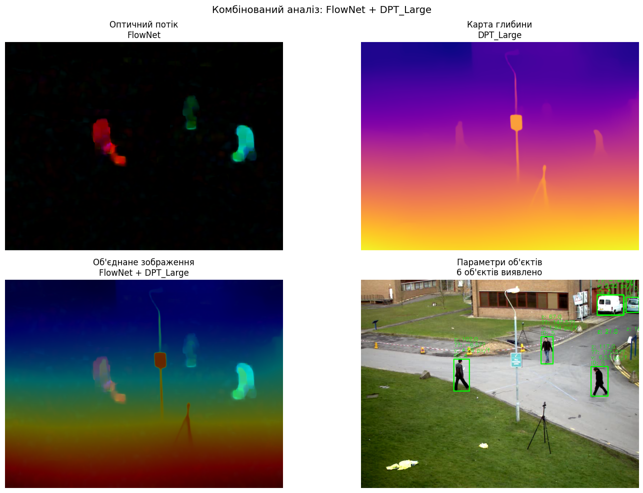
\includegraphics[width=6in,height=4.59565in]{media/image9.png}
\caption{Рис. 4.37 --- FlowNet\_DPT\_Large}
\end{figure}

На рис. 4.37 наведено результат «FlowNet\_DPT\_Large», який
використовується для порівняння оптичного потоку, карти глибини та
об'єднаного представлення сцени під час дистанційної ідентифікації
параметрів динамічних об'єктів.

На рис. 4.38 зображено FlowNet\_GeoNet. Комбінований аналіз: FlowNet +
GeoNet.

На рис. 4.38 показано результати роботи системи з використанням
нейромережевого алгоритму оптичного потоку FlowNet для оцінки руху та
моделі GeoNet для оцінки глибини сцени. Ця комбінація поєднує високу
точність нейромережевої оцінки руху з інтегрованим підходом до оцінки
глибини, що забезпечує просторово-часову узгодженість.

Ліва панель оптичний потік (FlowNet).

Ключові особливості FlowNet:

-- стійкість до оклюзій завдяки узагальнюючій здатності CNN;

-- деталізація дрібних рухів.

Центральна панель -- карта глибини (GeoNet).

Оцінка глибини виконана моделлю GeoNet -- глибокою нейронною
архітектурою, яка поєднує задачу оцінки глибини (DepthNet), пози камери
(PoseNet) та оптичного потоку (ResFlowNet) в єдиній неконтрольованій
(unsupervised) структурі. Ключові особливості GeoNet:

-- Спільне навчання: одночасне навчання оцінки глибини, пози та
оптичного потоку без використання розмічених даних.

-- Фотометрична узгодженість: функція втрат базується на реконструкції
кадрів, що забезпечує природну узгодженість між глибиною та рухом.

-- Геометрична коректність: карта глибини є фізично правдоподібною.

Порівняно з DPT\_Large, GeoNet дає дещо нижчу роздільну здатність, але
забезпечує кращу узгодженість між глибиною та оптичним потоком, оскільки
обидві задачі вирішуються спільно. Це особливо важливо для сцен зі
складним рухом камери. Кольорова шкала: теплі тони (жовтий,
помаранчевий, червоний) -- ближні об'єкти, холодні тони (зелений, синій,
фіолетовий) -- віддалені.

Права панель -- об'єднане зображення (FlowNet + GeoNet).

Накладання нейромережевого оптичного потоку FlowNet на карту глибини
GeoNet. Насиченість → інтенсивність руху, яскравість → глибина. Оскільки
GeoNet навчається спільно з оптичним потоком, його карта глибини
природно узгоджується з рухом. Це дозволяє:

- більш точно визначати просторове положення рухомих об'єктів;

- розрізняти власний рух об'єкта від руху камери;

- зменшувати помилки на межах об'єктів.

Детекція об'єктів.

Виявлено 6 об'єктів моделлю DETR. Поєднання з FlowNet + GeoNet дозволяє
обчислити повний набір параметрів (x, y, z, v, θ) з урахуванням
узгодженості між рухом та глибиною, що особливо важливо для сцен з
рухомою камерою.

\begin{figure}
\centering
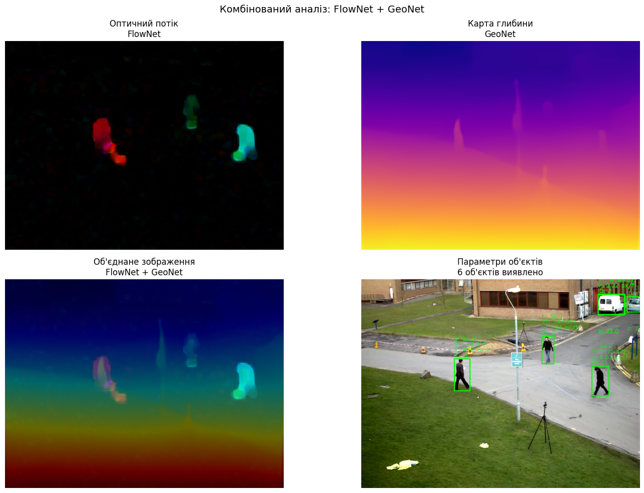
\includegraphics[width=6in,height=4.59207in]{media/image34.png}
\caption{Рис. 4.38 --- FlowNet\_GeoNet}
\end{figure}

На рис. 4.38 наведено результат «FlowNet\_GeoNet», який використовується
для порівняння оптичного потоку, карти глибини та об'єднаного
представлення сцени під час дистанційної ідентифікації параметрів
динамічних об'єктів.

На рис. 4.39 зображено FlowNet\_Gradient. Комбінований аналіз: FlowNet +
Gradient.

На рис. 4.39 показано результати роботи системи з використанням
нейромережевого алгоритму оптичного потоку FlowNet для оцінки руху та
методу градієнта (Gradient) для оцінки глибини сцени. Ця комбінація
демонструє можливості використання градієнтних методів для виділення меж
об'єктів при високоякісній оцінці оптичного потоку.

Ліва панель -- оптичний потік (FlowNet).

Ключові особливості FlowNet:

-- стійкість до оклюзій завдяки узагальнюючій здатності CNN;

-- деталізація дрібних рухів.

Центральна панель -- карта глибини (Gradient).

Оцінка глибини виконана методом градієнта (обчислення лапласіана або
модуля градієнта зображення). Цей метод ґрунтується на припущенні, що
різкі перепади яскравості відповідають межам об'єктів. Математично
градієнт зображення обчислюється як:

Особливості методу Gradient:

-- Чутливість до текстури: на текстурних областях (наприклад, трава,
листя) градієнт може бути високим навіть за відсутності перепаду
глибини.

На центральній панелі видно, що метод Gradient виділяє лише контури
об'єктів, а внутрішні області є однорідними.

Права панель -- об'єднане зображення (FlowNet + Gradient).

Накладання нейромережевого оптичного потоку FlowNet на градієнтну карту.
Насиченість → інтенсивність руху, яскравість → градієнт. Вектори потоку
чітко видно лише на межах об'єктів (там, де градієнт максимальний). Це
дозволяє аналізувати рух саме меж об'єктів, але не дає інформації про
рух внутрішніх точок. Незважаючи на високу якість оптичного потоку
FlowNet, відсутність абсолютних значень глибини обмежує практичне
застосування цієї комбінації.

Детекція об'єктів.

Виявлено 6 об'єктів моделлю DETR. Однак через відсутність абсолютних
значень глибини, визначення просторового положення об'єктів (координата
Z) є неможливим, незважаючи на високу точність виявлення та оцінки руху.

\begin{figure}
\centering
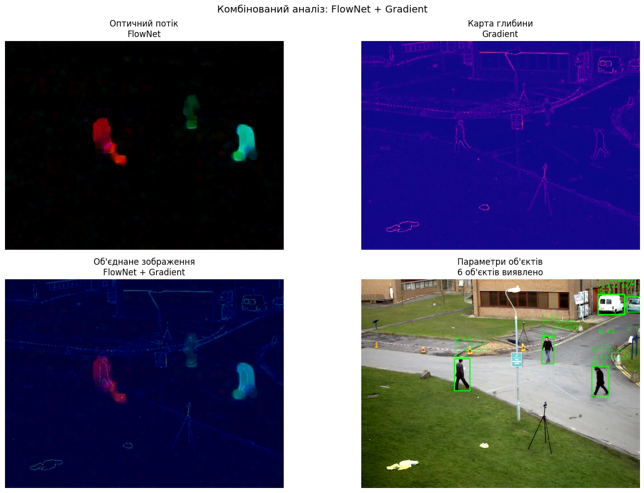
\includegraphics[width=6in,height=4.59207in]{media/image35.png}
\caption{Рис. 4.39 --- FlowNet\_Gradient}
\end{figure}

На рис. 4.39 наведено результат «FlowNet\_Gradient», який
використовується для порівняння оптичного потоку, карти глибини та
об'єднаного представлення сцени під час дистанційної ідентифікації
параметрів динамічних об'єктів.

На рис. 4.40 зображено FlowNet\_MiDaS. На рис. 4.40 показано результати
роботи системи з використанням нейромережевого алгоритму оптичного
потоку FlowNet для оцінки руху та нейромережевої моделі MiDaS для оцінки
глибини сцени. Ця комбінація є високоефективною, оскільки поєднує два
нейромережеві підходи: спеціалізовану мережу для оптичного потоку та
універсальну мережу для монокулярної оцінки глибини.

Ліва панель -- оптичний потік (FlowNet).

Ключові особливості FlowNet:

-- стійкість до оклюзій завдяки узагальнюючій здатності CNN;

-- деталізація дрібних рухів.

Центральна панель -- карта глибини (MiDaS).

Оцінка глибини виконана моделлю MiDaS (Mixed Depth and Stereo) --
нейромережевою архітектурою для монокулярної оцінки глибини. Ключові
характеристики MiDaS:

- Фізична коректність: карта глибини відображає реальну просторову
структуру сцени. Кольорова шкала: теплі тони (жовтий, помаранчевий,
червоний) -- ближні об'єкти, холодні тони (зелений, синій, фіолетовий)
-- віддалені.

- Чіткі межі об'єктів: перепади глибини на межах об'єктів є добре
помітними.

-- Робастність: MiDaS працює на різноманітних сценах без донавчання
(zero-shot).

-- Швидкодія: оптимізована версія MiDaS (MiDaS\_small) здатна працювати
в реальному часі на сучасних GPU.

На центральній панелі видно, що MiDaS коректно визначає глибину: близькі
об'єкти мають теплі кольори, віддалені -- холодні. Переходи глибини є
плавними, без різких артефактів.

Права панель -- об'єднане зображення (FlowNet + MiDaS). Накладання
нейромережевого оптичного потоку FlowNet на карту глибини MiDaS.
Насиченість → інтенсивність руху, яскравість → глибина. Це дозволяє
одночасно аналізувати напрямок, швидкість, відстань та просторове
положення об'єктів. Поєднання двох нейромережевих підходів дає високу
точність та надійність.

Детекція об'єктів. Виявлено 6 об'єктів моделлю DETR. Поєднання з FlowNet
+ MiDaS дозволяє обчислити повний набір параметрів (x, y, z, v, θ) з
високою точністю.

\begin{figure}
\centering
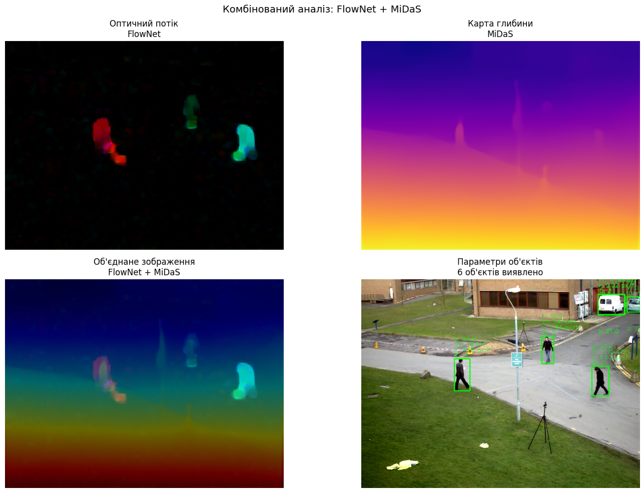
\includegraphics[width=6in,height=4.59207in]{media/image36.png}
\caption{Рис. 4.40 --- FlowNet\_MiDaS}
\end{figure}

На рис. 4.40 наведено результат «FlowNet\_MiDaS», який використовується
для порівняння оптичного потоку, карти глибини та об'єднаного
представлення сцени під час дистанційної ідентифікації параметрів
динамічних об'єктів.

\subsubsection{4.4.3 Результати поєднання методу GeoNet, методів
оцінювання глибини і
трансформерів}\label{ux440ux435ux437ux443ux43bux44cux442ux430ux442ux438-ux43fux43eux454ux434ux43dux430ux43dux43dux44f-ux43cux435ux442ux43eux434ux443-geonet-ux43cux435ux442ux43eux434ux456ux432-ux43eux446ux456ux43dux44eux432ux430ux43dux43dux44f-ux433ux43bux438ux431ux438ux43dux438-ux456-ux442ux440ux430ux43dux441ux444ux43eux440ux43cux435ux440ux456ux432}

На рис. 4.41 зображено GeoNet\_Bagging. На рис. 4.41 показано результати
роботи системи з використанням інтегрованої моделі GeoNet для оцінки
оптичного потоку та ансамблевого методу бегінгу (Bagging) для оцінки
глибини сцени. Ця комбінація поєднує переваги просторово-часової
узгодженості GeoNet з ансамблевим підвищенням стійкості оцінки глибини.

Ліва панель -- оптичний потік (GeoNet).

Поле оптичного потоку отримане моделлю GeoNet -- глибокою нейронною
архітектурою, яка поєднує задачу оцінки глибини (DepthNet), пози камери
(PoseNet) та оптичного потоку (ResFlowNet) в єдиній неконтрольованій
(unsupervised) структурі. Ключові особливості GeoNet для оцінки
оптичного потоку:

-- Узгодженість з глибиною: оскільки мережа навчається спільно, оптичний
потік природно узгоджується з картою глибини.

- Відокремлення руху камери: здатність розрізняти власний рух об'єкта
від руху камери.

-- Геометрична коректність: потік задовольняє епіполярним обмеженням для
статичних сцен.

Кольорове кодування: червоно-жовті тони → рух вправо/вверх, синьо-зелені
→ вліво/вниз; насиченість → інтенсивність руху.

Центральна панель -- карта глибини (Bagging).

Переваги Bagging:

-- Зменшення дисперсії: локальні шумові викиди на карті глибини
згладжуються за рахунок усереднення.

-- Підвищення стійкості: ансамбль менш чутливий до аномалій в окремих
кадрах.

-- Збереження структури: основні просторові структури сцени
зберігаються.

Кольорова шкала: теплі тони (жовтий, помаранчевий, червоний) -- ближні
об'єкти, холодні тони (зелений, синій, фіолетовий) -- віддалені.

Права панель -- об'єднане зображення (GeoNet + Bagging).

Накладання оптичного потоку GeoNet на ансамблеву карту глибини Bagging.
Насиченість → інтенсивність руху, яскравість → глибина. Поєднання
узгодженого потоку GeoNet зі згладженою ансамблевою глибиною забезпечує:

-- високу стійкість до шумів завдяки Bagging;

-- просторово-часову узгодженість завдяки GeoNet;

-- надійне визначення параметрів руху та глибини.

Детекція об'єктів.

Виявлено 6 об'єктів моделлю DETR. Поєднання з GeoNet + Bagging дозволяє
обчислити повний набір параметрів (x, y, z, v, θ) з високою стійкістю до
шумів та узгодженістю між рухом та глибиною.

\begin{figure}
\centering
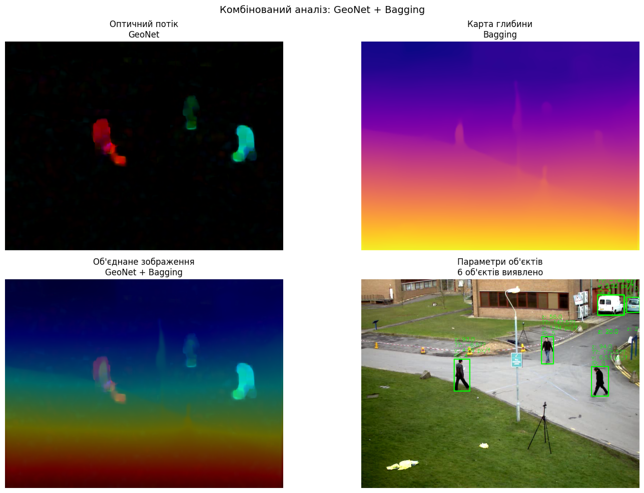
\includegraphics[width=6in,height=4.59207in]{media/image37.png}
\caption{Рис. 4.41 --- GeoNet\_Bagging}
\end{figure}

На рис. 4.41 наведено результат «GeoNet\_Bagging», який використовується
для порівняння оптичного потоку, карти глибини та об'єднаного
представлення сцени під час дистанційної ідентифікації параметрів
динамічних об'єктів.

На рис. 4.42 зображено GeoNet\_Blur. На рис. 4.42 показано результати
роботи системи з використанням інтегрованої моделі GeoNet для оцінки
оптичного потоку та простого методу розмиття (Blur) для оцінки глибини
сцени. Ця комбінація демонструє, що навіть при використанні найкращих
методів оцінки руху, низька якість оцінки глибини суттєво обмежує
загальну ефективність системи.

Ліва панель -- оптичний потік (GeoNet).

Поле оптичного потоку отримане моделлю GeoNet 8 -- глибокою нейронною
архітектурою, яка поєднує задачу оцінки глибини (DepthNet), пози камери
(PoseNet) та оптичного потоку (ResFlowNet) в єдиній неконтрольованій
(unsupervised) структурі. Згідно з оригінальною роботою, GeoNet
використовує фотометричну узгодженість для навчання: карта глибини та
оптичний потік навчаються спільно через реконструкцію кадрів.

Ключові особливості GeoNet для оцінки оптичного потоку:

- Відокремлення руху камери: здатність розрізняти власний рух об'єкта
від руху камери завдяки PoseNet.

Центральна панель -- карта глибини (Blur).

- Відсутність фізичної коректності: карта глибини є лише згладженою
версією яскравісного каналу зображення, яка не має зв'язку з реальною
відстанню до об'єктів.

- Розмиті межі: на відміну від методу Gradient, який виділяє межі, Blur
їх розмиває, що унеможливлює точну сегментацію об'єктів.

- Відсутність кореляції з реальною глибиною: близький об'єкт може мати
холодний колір, а віддалений -- теплий.

Цей метод є «нижньою межею» якості оцінки глибини.

Права панель -- об'єднане зображення (GeoNet + Blur).

Накладання оптичного потоку GeoNet на карту глибини Blur. Насиченість →
інтенсивність руху, яскравість → псевдо-глибина. Оскільки карта глибини
не має фізичного сенсу, об'єднане зображення вводить в оману, незважаючи
на високу якість оптичного потоку GeoNet. Узгодженість між потоком та
глибиною, яка є ключовою перевагою GeoNet, повністю нівелюється низькою
якістю методу Blur.

Детекція об'єктів.

Виявлено 6 об'єктів моделлю DETR. Однак через відсутність фізично
коректної глибини, визначення просторового положення об'єктів
(координата Z) є неможливим, незважаючи на високу точність виявлення та
оцінки руху.

\begin{figure}
\centering
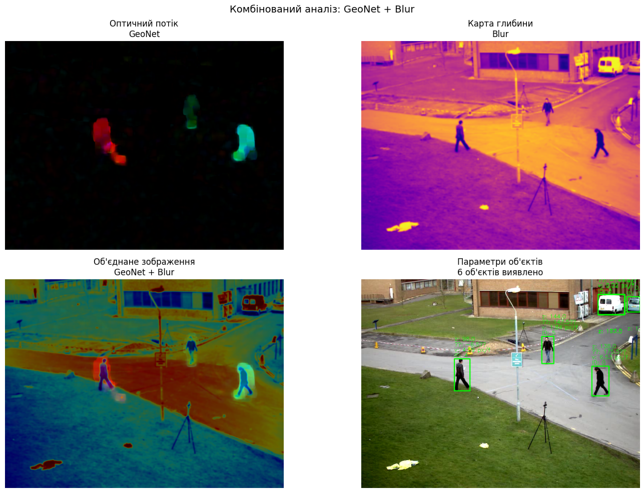
\includegraphics[width=6in,height=4.59207in]{media/image38.png}
\caption{Рис. 4.42 --- GeoNet\_Blur}
\end{figure}

На рис. 4.42 наведено результат «GeoNet\_Blur», який використовується
для порівняння оптичного потоку, карти глибини та об'єднаного
представлення сцени під час дистанційної ідентифікації параметрів
динамічних об'єктів.

На рис. 4.43 зображено GeoNet\_Boosting. На рис. 4.43 показано
результати роботи системи з використанням інтегрованої моделі GeoNet для
оцінки оптичного потоку та ансамблевого методу бустінгу для оцінки
глибини сцени. Ця комбінація поєднує просторово-часову узгодженість
GeoNet з ансамблевим підвищенням точності та підкресленням меж об'єктів.

Ліва панель -- оптичний потік (GeoNet).

Поле оптичного потоку отримане моделлю GeoNet 8 -- глибокою нейронною
архітектурою, яка поєднує задачу оцінки глибини (DepthNet), пози камери
(PoseNet) та оптичного потоку (ResFlowNet) в єдиній неконтрольованій
(unsupervised) структурі. Згідно з оригінальною роботою, GeoNet
використовує фотометричну узгодженість для навчання.

Ключові особливості GeoNet:

-- Узгодженість з глибиною: спільне навчання забезпечує природну
узгодженість між потоком та глибиною.

Центральна панель -- карта глибини (Boosting).

Оцінка глибини виконана ансамблевим методом бустінгу. На відміну від
бегінгу (Bagging), який усереднює результати паралельних моделей,
бустінг передбачає послідовне навчання моделей, де кожна наступна
фокусується на виправленні помилок попередньої. Математично це
виражається як зважене підсумовування:

\[D_{boost} = \ \Sigma(m = 1..M)\alpha_{m}D^{m},\ \alpha_{m} = \frac{1}{2}\ln\left( \frac{1\  - \ \varepsilon_{m}}{\varepsilon_{m}} \right)\]

де \(\alpha_{m}\) -- вага, обернено пропорційна помилці
\(\varepsilon_{m}\).

Права панель -- об'єднане зображення (GeoNet + Boosting).

Накладання оптичного потоку GeoNet на карту глибини Boosting.
Насиченість → інтенсивність руху, яскравість → глибина. Поєднання
узгодженого потоку GeoNet з підкресленими межами Boosting дозволяє:

- чітко відокремлювати об'єкти один від одного навіть при частковому
перекритті;

- точно визначати просторове положення рухомих об'єктів;

- розрізняти власний рух об'єкта від руху камери.

Детекція об'єктів.

Виявлено 6 об'єктів моделлю DETR. Поєднання з GeoNet + Boosting дозволяє
обчислити повний набір параметрів (x, y, z, v, θ) з високою точністю,
особливо на межах об'єктів та в сценах з рухомою камерою.

\begin{figure}
\centering
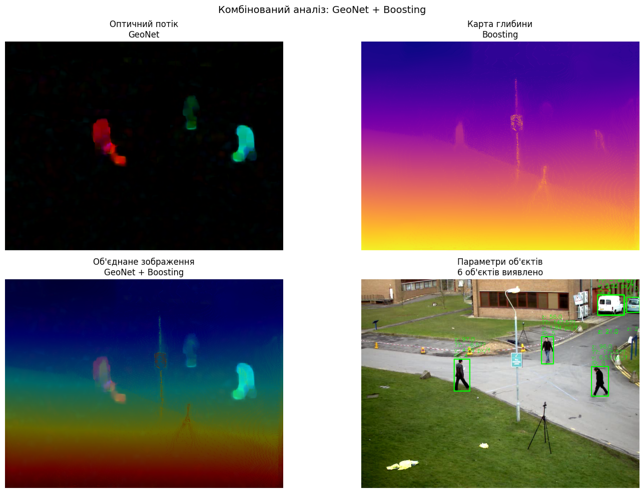
\includegraphics[width=6in,height=4.59207in]{media/image39.png}
\caption{Рис. 4.43 --- GeoNet\_Boosting}
\end{figure}

На рис. 4.43 наведено результат «GeoNet\_Boosting», який
використовується для порівняння оптичного потоку, карти глибини та
об'єднаного представлення сцени під час дистанційної ідентифікації
параметрів динамічних об'єктів.

На рис. 4.44 зображено GeoNet\_DPT\_Large. Комбінований аналіз: GeoNet +
DPT\_Large.

На рис. 4.44 показано результати роботи системи з використанням
інтегрованої моделі GeoNet для оцінки оптичного потоку та трансформерної
моделі DPT\_Large для оцінки глибини сцени. Ця комбінація поєднує
просторово-часову узгодженість GeoNet з високою роздільною здатністю
DPT\_Large.

Ліва панель -- оптичний потік (GeoNet).

Ключові особливості GeoNet:

Центральна панель -- карта глибини (DPT\_Large).

- Дуже висока роздільна здатність: модель зберігає деталі дрібних
об'єктів (гілки дерев, дрібні конструкції).

Права панель -- об'єднане зображення (GeoNet + DPT\_Large).

Накладання оптичного потоку GeoNet на високороздільну карту глибини
DPT\_Large. Насиченість → інтенсивність руху, яскравість → глибина.
Поєднання узгодженого потоку GeoNet з високою роздільною здатністю
DPT\_Large дозволяє:

- одночасно аналізувати напрямок, швидкість, відстань та просторове
положення навіть для дрібних об'єктів;

- розрізняти власний рух об'єкта від руху камери завдяки GeoNet;

- чітко відокремлювати об'єкти, що частково перекриваються (оклюзії).

Детекція об'єктів.

Виявлено 6 об'єктів моделлю DETR. Поєднання з GeoNet + DPT\_Large
дозволяє обчислити повний набір параметрів (x, y, z, v, θ) з високою
точністю, роздільною здатністю та просторово-часовою узгодженістю.

\begin{figure}
\centering
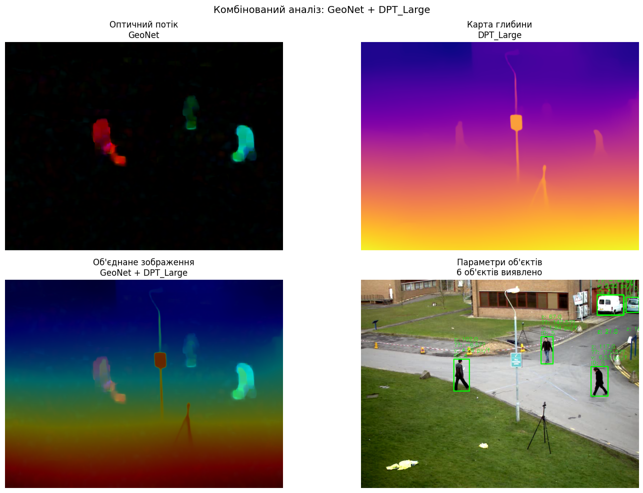
\includegraphics[width=6in,height=4.59565in]{media/image40.png}
\caption{Рис. 4.44 --- GeoNet\_DPT\_Large}
\end{figure}

На рис. 4.44 наведено результат «GeoNet\_DPT\_Large», який
використовується для порівняння оптичного потоку, карти глибини та
об'єднаного представлення сцени під час дистанційної ідентифікації
параметрів динамічних об'єктів.

На рис. 4.45 зображено GeoNet\_GeoNet. На рис. 4.45 показано результати
роботи системи з використанням інтегрованої моделі GeoNet для одночасної
оцінки оптичного потоку та глибини сцени. Ця комбінація є унікальною,
оскільки обидві оцінки виконуються єдиною моделлю, що забезпечує
максимальну просторово-часову узгодженість.

Ліва панель -- оптичний потік (GeoNet).

Ключові особливості GeoNet для оцінки оптичного потоку:

Центральна панель -- карта глибини (GeoNet).

Оцінка глибини виконана тією ж моделлю GeoNet. В оригінальній роботі
GeoNet використовує два ключові модулі для забезпечення геометричної
узгодженості:

Depth-to-Normal Network: використовує розв'язок задачі найменших
квадратів для обчислення поверхневої нормалі з карти глибини:

\[n\  = \frac{\left( \left( A^{T}A \right)^{- 1}A^{T}1 \right)}{}\left| \left| \left( A^{T}A \right)^{- 1}A^{T}1 \right| \right|\]

Normal-to-Depth Network: оновлює оцінку глибини через ядерну регресію на
основі нормалей:

\[z_{i} = \frac{\left( \Sigma\left( j \in M_{i} \right)K\left( n_{j},n_{i} \right)z_{ji}' \right)}{}\left( \Sigma\left( j \in M_{i} \right)K\left( n_{j},n_{i} \right) \right)\]

Права панель -- об'єднане зображення (GeoNet + GeoNet).

Накладання оптичного потоку GeoNet на карту глибини GeoNet. Насиченість
→ інтенсивність руху, яскравість → глибина. Оскільки обидві оцінки
походять з однієї моделі, вони максимально узгоджені: вектори потоку
ідеально вирівняні з градієнтом глибини. Це дозволяє:

- точно розрізняти власний рух об'єкта від руху камери;

- зменшувати помилки на межах об'єктів, де класичні методи
«розтікаються»;

-- забезпечувати фізично коректну просторово-часову узгодженість.

Детекція об'єктів.

Виявлено 6 об'єктів моделлю DETR. Поєднання з GeoNet + GeoNet дозволяє
обчислити повний набір параметрів (x, y, z, v, θ) з максимальною
узгодженістю між рухом та глибиною, що особливо важливо для сцен з
рухомою камерою.

\begin{figure}
\centering
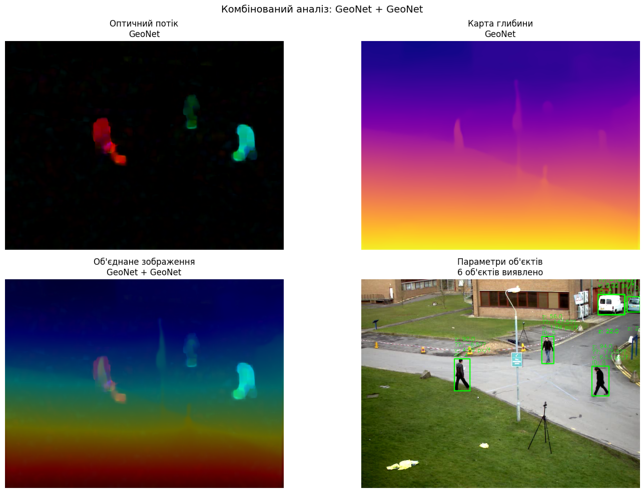
\includegraphics[width=6in,height=4.59207in]{media/image10.png}
\caption{Рис. 4.45 --- GeoNet\_GeoNet}
\end{figure}

На рис. 4.45 наведено результат «GeoNet\_GeoNet», який використовується
для порівняння оптичного потоку, карти глибини та об'єднаного
представлення сцени під час дистанційної ідентифікації параметрів
динамічних об'єктів.

На рис. 4.46 зображено GeoNet\_Gradient. На рис. 4.46 показано
результати роботи системи з використанням інтегрованої моделі GeoNet для
оцінки оптичного потоку та методу градієнта (Gradient) для оцінки
глибини сцени. Ця комбінація демонструє можливості використання
градієнтних методів для виділення меж об'єктів при високоякісній
узгодженій оцінці оптичного потоку.

Ліва панель -- оптичний потік (GeoNet).

Поле оптичного потоку отримане моделлю GeoNet 8 -- глибокою нейронною
архітектурою, яка поєднує задачу оцінки глибини (DepthNet), пози камери
(PoseNet) та оптичного потоку (ResFlowNet) в єдиній неконтрольованій
(unsupervised) структурі.

Ключові особливості GeoNet:

Центральна панель -- карта глибини (Gradient).

Оцінка глибини виконана методом градієнта (обчислення лапласіана або
модуля градієнта зображення). Математично градієнт зображення
обчислюється як:

Особливості методу Gradient:

-- Чутливість до текстури: на текстурних областях градієнт може бути
високим навіть за відсутності перепаду глибини.

Права панель -- об'єднане зображення (GeoNet + Gradient).

Накладання оптичного потоку GeoNet на градієнтну карту. Насиченість →
інтенсивність руху, яскравість → градієнт. Вектори потоку чітко видно
лише на межах об'єктів (там, де градієнт максимальний). Це дозволяє
аналізувати рух саме меж об'єктів, але не дає інформації про рух
внутрішніх точок. Незважаючи на високу узгодженість оптичного потоку
GeoNet, відсутність абсолютних значень глибини обмежує практичне
застосування цієї комбінації.

Детекція об'єктів.

Виявлено 6 об'єктів моделлю DETR. Однак через відсутність абсолютних
значень глибини, визначення просторового положення об'єктів (координата
Z) є неможливим, незважаючи на високу якість узгодженого оптичного
потоку GeoNet.

\begin{figure}
\centering
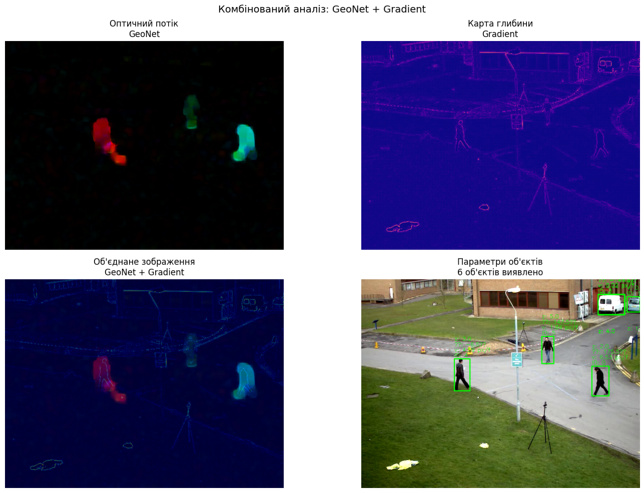
\includegraphics[width=6in,height=4.59207in]{media/image41.png}
\caption{Рис. 4.46 --- GeoNet\_Gradient}
\end{figure}

На рис. 4.46 наведено результат «GeoNet\_Gradient», який
використовується для порівняння оптичного потоку, карти глибини та
об'єднаного представлення сцени під час дистанційної ідентифікації
параметрів динамічних об'єктів.

На рис. 4.47 зображено GeoNet\_MiDaS. На рис. 4.47 показано результати
роботи системи з використанням інтегрованої моделі GeoNet для оцінки
оптичного потоку та нейромережевої моделі MiDaS для оцінки глибини
сцени. Ця комбінація поєднує просторово-часову узгодженість GeoNet з
універсальністю та хорошою якістю MiDaS.

Ліва панель -- оптичний потік (GeoNet).

Ключові особливості GeoNet:

Центральна панель -- карта глибини (MiDaS).

-- Фізична коректність: карта глибини відображає реальну просторову
структуру сцени.

- Чіткі межі об'єктів: перепади глибини на межах об'єктів є добре
помітними.

-- Робастність: MiDaS працює на різноманітних сценах без донавчання
(zero-shot).

-- Швидкодія: оптимізована версія MiDaS здатна працювати в реальному
часі.

Права панель -- об'єднане зображення (GeoNet + MiDaS).

Накладання оптичного потоку GeoNet на карту глибини MiDaS. Насиченість →
інтенсивність руху, яскравість → глибина. Поєднання узгодженого потоку
GeoNet з якісною глибиною MiDaS дозволяє:

- аналізувати напрямок, швидкість та просторове положення об'єктів;

-- отримувати фізично коректну просторову інформацію завдяки MiDaS.

Детекція об'єктів.

Виявлено 6 об'єктів моделлю DETR. Поєднання з GeoNet + MiDaS дозволяє
обчислити повний набір параметрів (x, y, z, v, θ) з узгодженістю між
рухом та глибиною, що особливо важливо для сцен з рухомою камерою.

\begin{figure}
\centering
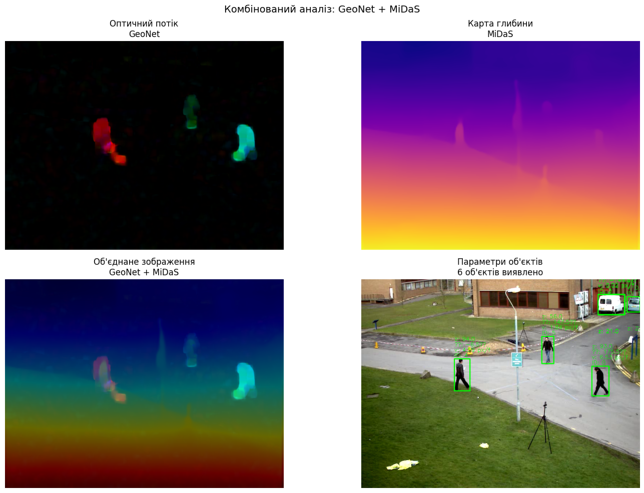
\includegraphics[width=6in,height=4.59207in]{media/image42.png}
\caption{Рис. 4.47 --- GeoNet\_MiDaS}
\end{figure}

На рис. 4.47 наведено результат «GeoNet\_MiDaS», який використовується
для порівняння оптичного потоку, карти глибини та об'єднаного
представлення сцени під час дистанційної ідентифікації параметрів
динамічних об'єктів.

\subsubsection{4.4.4 Результати поєднання методу Horn--Schunck, методів
оцінювання глибини і
трансформерів}\label{ux440ux435ux437ux443ux43bux44cux442ux430ux442ux438-ux43fux43eux454ux434ux43dux430ux43dux43dux44f-ux43cux435ux442ux43eux434ux443-hornschunck-ux43cux435ux442ux43eux434ux456ux432-ux43eux446ux456ux43dux44eux432ux430ux43dux43dux44f-ux433ux43bux438ux431ux438ux43dux438-ux456-ux442ux440ux430ux43dux441ux444ux43eux440ux43cux435ux440ux456ux432}

На рис. 4.48 зображено HornSchunck\_Bagging. Комбінований аналіз:
HornSchunck + Bagging.

На рис. 4.48 показано результати роботи системи з використанням
класичного глобального алгоритму оптичного потоку Горна--Шунка
(Horn--Schunck) для оцінки руху та ансамблевого методу бегінгу (Bagging)
для оцінки глибини сцени. Ця комбінація поєднує глобальну гладкість
оцінки руху з ансамблевим підвищенням стійкості оцінки глибини.

Ліва панель -- оптичний потік (Horn--Schunck).

Поле оптичного потоку отримане методом Горна--Шунка 19 -- першим
глобальним підходом до оцінки оптичного потоку. Згідно з оригінальною
роботою, метод мінімізує функціонал енергії, що поєднує дані та
гладкість:

\[E(u,v) = \ \iint_{}^{}{\left( I_{x}u\  + \ I_{y}v\  + \ I(t) \right)^{2}dx}dy\  + \ \alpha^{2}\iint_{}^{}{\left( |\nabla u|^{2} + \ |\nabla v|^{2} \right)dx}dy\]

де перший член (дані) штрафує відхилення від рівняння яскравості, другий
(гладкість) -- швидкі зміни поля потоку, а α -- коефіцієнт
регуляризації.

Ключові особливості методу Горна--Шунка:

-- Глобальна гладкість: на відміну від локальних методів
(Лукаса--Канаде), Horn--Schunck дає густе поле потоку з плавними
переходами між сусідніми пікселями.

-- Стійкість у однорідних областях: там, де градієнт яскравості малий,
інформація «заповнюється» від меж завдяки гладкості.

- Чутливість до шумів: метод може розмивати межі рухомих об'єктів через
квадратичну регуляризацію.

Ітераційна схема розв'язання (метод Якобі) має вигляд:

\[u^{k + 1} = \ ū^{k} - \frac{\left\lbrack I_{x}\left( I_{x}ū^{k} + \ I_{y}{\bar{v}}^{k} + \ I(t) \right) \right\rbrack}{}\left\lbrack \alpha^{2} + \ I_{x}^{2} + \ I_{y}^{2} \right\rbrack\]

\[v^{k + 1} = \ {\bar{v}}^{k} - \frac{\left\lbrack I_{y}\left( I_{x}ū^{k} + \ I_{y}{\bar{v}}^{k} + \ I(t) \right) \right\rbrack}{}\left\lbrack \alpha^{2} + \ I_{x}^{2} + \ I_{y}^{2} \right\rbrack\]

де \(ū^{k}\), \({\bar{v}}^{k}\) -- середні значення сусідніх пікселів на
k-й ітерації.

Центральна панель -- карта глибини (Bagging).

Переваги Bagging: зменшення дисперсії (локальні шумові викиди
згладжуються), підвищення стійкості до аномалій в окремих кадрах,
збереження просторової структури сцени. Кольорова шкала: теплі тони
(жовтий, помаранчевий, червоний) -- ближні об'єкти, холодні тони
(зелений, синій, фіолетовий) -- віддалені.

Права панель -- об'єднане зображення (Horn--Schunck + Bagging).

Накладання оптичного потоку Horn--Schunck на ансамблеву карту глибини
Bagging. Насиченість → інтенсивність руху, яскравість → глибина.
Поєднання глобально гладкого потоку Horn--Schunck зі згладженою
ансамблевою глибиною забезпечує високу стійкість до шумів, хоча метод
Horn--Schunck може розмивати межі швидко рухомих об'єктів.

Детекція об'єктів.

Виявлено 6 об'єктів моделлю DETR. Поєднання з Horn--Schunck + Bagging
дозволяє обчислити повний набір параметрів (x, y, z, v, θ) з підвищеною
стійкістю до шумів, особливо в однорідних областях з малим градієнтом
яскравості.

\begin{figure}
\centering
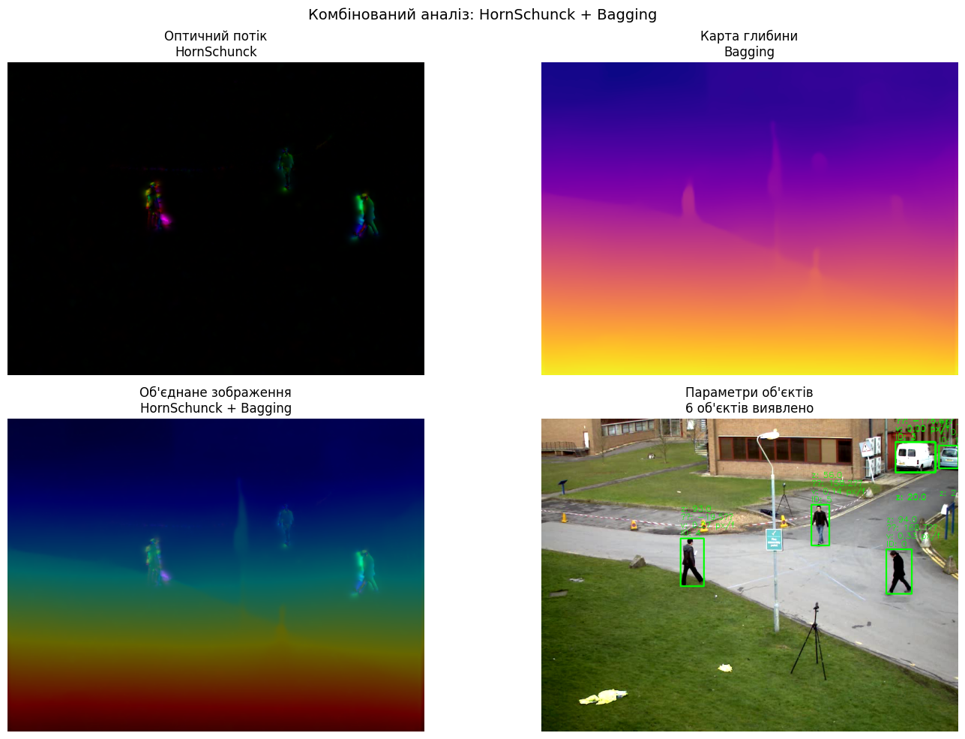
\includegraphics[width=6in,height=4.59207in]{media/image11.png}
\caption{Рис. 4.48 --- HornSchunck\_Bagging}
\end{figure}

На рис. 4.48 наведено результат «HornSchunck\_Bagging», який
використовується для порівняння оптичного потоку, карти глибини та
об'єднаного представлення сцени під час дистанційної ідентифікації
параметрів динамічних об'єктів.

На рис. 4.49 зображено HornSchunck\_Blur. Комбінований аналіз:
HornSchunck + Blur.

На рис. 4.49 показано результати роботи системи з використанням
класичного глобального алгоритму оптичного потоку Горна--Шунка
(Horn--Schunck) для оцінки руху та простого методу розмиття (Blur) для
оцінки глибини сцени. Ця комбінація демонструє, що навіть при
використанні глобального методу оптичного потоку, низька якість оцінки
глибини суттєво обмежує загальну ефективність системи.

Ліва панель -- оптичний потік (Horn--Schunck).

де перший член дані штрафує відхилення від рівняння яскравості, другий
гладкість швидкі зміни поля потоку, а \(\alpha\) -- коефіцієнт
регуляризації.

Ключові особливості методу Горна--Шунка:

-- Глобальна гладкість: на відміну від локальних методів
(Лукаса--Канаде), Horn--Schunck дає густе поле потоку з плавними
переходами.

- Чутливість до шумів та розмиття меж: метод може розмивати межі рухомих
об'єктів через квадратичну регуляризацію.

Центральна панель -- карта глибини (Blur).

-- Відсутність фізичної коректності: карта глибини є лише згладженою
версією яскравісного каналу зображення.

- Розмиті межі: метод не виділяє межі об'єктів, що унеможливлює точну
сегментацію.

Цей метод є «нижньою межею» якості оцінки глибини.

Права панель -- об'єднане зображення (Horn--Schunck + Blur).

Накладання оптичного потоку Horn--Schunck на карту глибини Blur.
Насиченість → інтенсивність руху, яскравість → псевдо-глибина. Оскільки
карта глибини не має фізичного сенсу, об'єднане зображення вводить в
оману, незважаючи на глобальну гладкість оптичного потоку Horn--Schunck.
Глобальна регуляризація Horn--Schunck, яка є його перевагою в однорідних
областях, не може компенсувати відсутність якісної глибини.

Детекція об'єктів.

Виявлено 6 об'єктів моделлю DETR. Однак через відсутність фізично
коректної глибини, визначення просторового положення об'єктів
(координата Z) є неможливим, незважаючи на глобальну гладкість оцінки
руху.

\begin{figure}
\centering
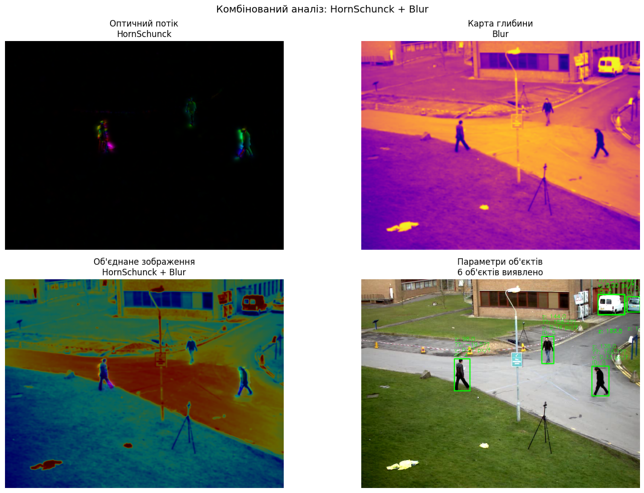
\includegraphics[width=6in,height=4.59207in]{media/image43.png}
\caption{Рис. 4.49 --- HornSchunck\_Blur}
\end{figure}

На рис. 4.49 наведено результат «HornSchunck\_Blur», який
використовується для порівняння оптичного потоку, карти глибини та
об'єднаного представлення сцени під час дистанційної ідентифікації
параметрів динамічних об'єктів.

На рис. 4.50 зображено HornSchunck\_Boosting. Комбінований аналіз:
HornSchunck + Boosting.

На рис. 4.50 показано результати роботи системи з використанням
класичного глобального алгоритму оптичного потоку Горна--Шунка
(Horn--Schunck) для оцінки руху та ансамблевого методу бустінгу для
оцінки глибини сцени. Ця комбінація поєднує глобальну гладкість оцінки
руху з ансамблевим підвищенням точності та підкресленням меж об'єктів.

Ліва панель -- оптичний потік (Horn--Schunck).

Ключові особливості методу Горна--Шунка:

Ітераційна схема розв'язання (метод Якобі):

Центральна панель -- карта глибини (Boosting).

\[D_{boost} = \ \Sigma(m = 1..M)\alpha_{m}D^{m},\ \alpha_{m} = \frac{1}{2}\ln\left( \frac{1\  - \ \varepsilon_{m}}{\varepsilon_{m}} \right)\]

де \(\alpha_{m}\) -- вага, обернено пропорційна помилці
\(\varepsilon_{m}\).

Права панель -- об'єднане зображення (Horn--Schunck + Boosting).

Накладання оптичного потоку Horn--Schunck на карту глибини Boosting.
Насиченість → інтенсивність руху, яскравість → глибина. Поєднання
глобально гладкого потоку Horn--Schunck з підкресленими межами Boosting
дозволяє компенсувати основний недолік методу Horn--Schunck -- розмиття
меж об'єктів. Однак через глобальну регуляризацію, Horn--Schunck все ще
може згладжувати різкі перепади швидкості на межах об'єктів.

Детекція об'єктів.

Виявлено 6 об'єктів моделлю DETR. Поєднання з Horn--Schunck + Boosting
дозволяє обчислити повний набір параметрів (\(x,\ y,\ z,\ v,\ \theta\))
з підвищеною точністю на межах об'єктів, частково компенсуючи основний
недолік глобального методу Горна--Шунка.

\begin{figure}
\centering
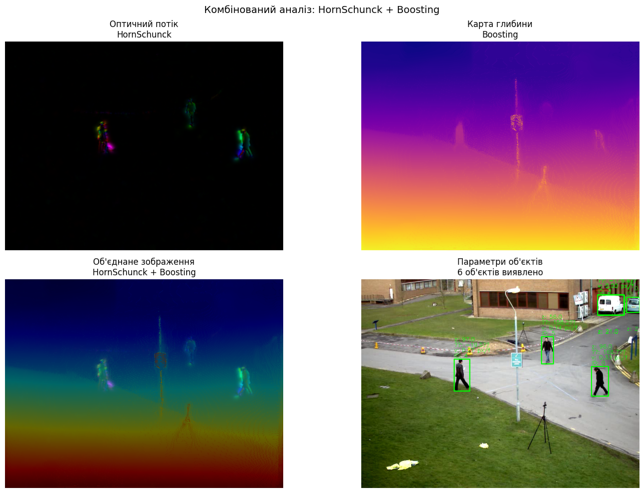
\includegraphics[width=6in,height=4.59207in]{media/image44.png}
\caption{Рис. 4.50 --- HornSchunck\_Boosting}
\end{figure}

На рис. 4.50 наведено результат «HornSchunck\_Boosting», який
використовується для порівняння оптичного потоку, карти глибини та
об'єднаного представлення сцени під час дистанційної ідентифікації
параметрів динамічних об'єктів.

На рис. 4.51 зображено HornSchunck\_DPT\_Large. Комбінований аналіз:
HornSchunck + DPT\_Large.

На рис. 4.51 показано результати роботи системи з використанням
класичного глобального алгоритму оптичного потоку Горна--Шунка
(Horn--Schunck) для оцінки руху та трансформерної моделі DPT\_Large для
оцінки глибини сцени. Ця комбінація поєднує глобальну гладкість оцінки
руху з високою роздільною здатністю та чіткими межами DPT\_Large.

Ліва панель -- оптичний потік (Horn--Schunck).

Ключові особливості методу Горна--Шунка:

Центральна панель -- карта глибини (DPT\_Large).

Права панель -- об'єднане зображення (Horn--Schunck + DPT\_Large).

Накладання оптичного потоку Horn--Schunck на високороздільну карту
глибини DPT\_Large. Насиченість → інтенсивність руху, яскравість →
глибина. Поєднання глобально гладкого потоку Horn--Schunck з високою
роздільною здатністю DPT\_Large дозволяє отримати фізично коректну
просторову інформацію. Однак основний недолік Horn--Schunck -- розмиття
меж швидко рухомих об'єктів -- не компенсується навіть високоякісною
глибиною, оскільки це властивість самого методу оптичного потоку.

Детекція об'єктів.

Виявлено 6 об'єктів моделлю DETR. Поєднання з Horn--Schunck + DPT\_Large
дозволяє обчислити повний набір параметрів (x, y, z, v, θ) з високою
якістю глибини, але з потенційним розмиттям меж у полі оптичного потоку.

\begin{figure}
\centering
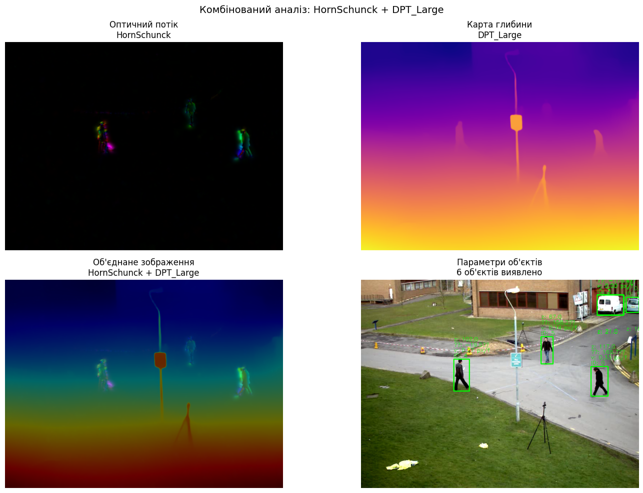
\includegraphics[width=6in,height=4.59565in]{media/image45.png}
\caption{Рис. 4.51 --- HornSchunck\_DPT\_Large}
\end{figure}

На рис. 4.51 наведено результат «HornSchunck\_DPT\_Large», який
використовується для порівняння оптичного потоку, карти глибини та
об'єднаного представлення сцени під час дистанційної ідентифікації
параметрів динамічних об'єктів.

На рис. 4.52 зображено HornSchunck\_GeoNet. Комбінований аналіз:
HornSchunck + GeoNet.

На рис. 4.52 показано результати роботи системи з використанням
класичного глобального алгоритму оптичного потоку Горна--Шунка
(Horn--Schunck) для оцінки руху та інтегрованої моделі GeoNet для оцінки
глибини сцени. Ця комбінація поєднує глобальну гладкість оцінки руху з
просторово-часовою узгодженістю GeoNet.

Ліва панель -- оптичний потік (Horn--Schunck).

Ключові особливості методу Горна--Шунка:

Центральна панель -- карта глибини (GeoNet).

Оцінка глибини виконана моделлю GeoNet 8 -- глибокою нейронною
архітектурою, яка поєднує задачу оцінки глибини (DepthNet), пози камери
(PoseNet) та оптичного потоку (ResFlowNet) в єдиній неконтрольованій
(unsupervised) структурі. Ключові особливості GeoNet:

-- Спільне навчання: одночасне навчання оцінки глибини, пози та
оптичного потоку.

-- Фотометрична узгодженість: функція втрат базується на реконструкції
кадрів.

-- Геометрична коректність: карта глибини є фізично правдоподібною.

Права панель -- об'єднане зображення (Horn--Schunck + GeoNet).

Накладання оптичного потоку Horn--Schunck на карту глибини GeoNet.
Насиченість → інтенсивність руху, яскравість → глибина. Поєднання
глобально гладкого потоку Horn--Schunck з узгодженою глибиною GeoNet
дозволяє отримати фізично коректну просторову інформацію. Однак основний
недолік Horn--Schunck -- розмиття меж швидко рухомих об'єктів -- не
компенсується навіть узгодженою глибиною GeoNet, оскільки це властивість
самого методу оптичного потоку.

Детекція об'єктів.

Виявлено 6 об'єктів моделлю DETR. Поєднання з Horn--Schunck + GeoNet
дозволяє обчислити повний набір параметрів (x, y, z, v, θ) з
узгодженістю між рухом та глибиною, але з потенційним розмиттям меж у
полі оптичного потоку.

\begin{figure}
\centering
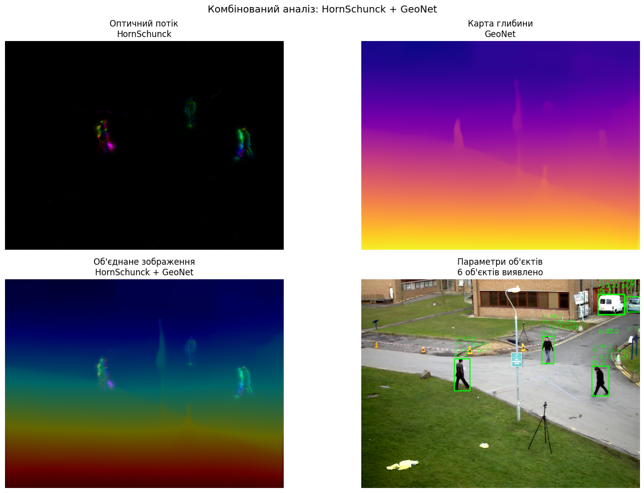
\includegraphics[width=6in,height=4.59207in]{media/image46.png}
\caption{Рис. 4.52 --- HornSchunck\_GeoNet}
\end{figure}

На рис. 4.52 наведено результат «HornSchunck\_GeoNet», який
використовується для порівняння оптичного потоку, карти глибини та
об'єднаного представлення сцени під час дистанційної ідентифікації
параметрів динамічних об'єктів.

На рис. 4.53 зображено HornSchunck\_Gradient. Комбінований аналіз:
HornSchunck + Gradient.

На рис. 4.53 показано результати роботи системи з використанням
класичного глобального алгоритму оптичного потоку Горна--Шунка
(Horn--Schunck) для оцінки руху та методу градієнта (Gradient) для
оцінки глибини сцени. Ця комбінація демонструє можливості використання
градієнтних методів для виділення меж об'єктів при глобальній оцінці
оптичного потоку.

Ліва панель -- оптичний потік (Horn--Schunck).

Ключові особливості методу Горна--Шунка:

Центральна панель -- карта глибини (Gradient).

Особливості методу Gradient:

Права панель -- об'єднане зображення (Horn--Schunck + Gradient).

Накладання оптичного потоку Horn--Schunck на градієнтну карту.
Насиченість → інтенсивність руху, яскравість → градієнт. Вектори потоку
чітко видно лише на межах об'єктів (там, де градієнт максимальний). Це
дозволяє аналізувати рух саме меж об'єктів, але не дає інформації про
рух внутрішніх точок. Глобальна гладкість Horn--Schunck призводить до
того, що вектори потоку «розтікаються» від меж в однорідні області, де
градієнт відсутній.

Детекція об'єктів.

Виявлено 6 об'єктів моделлю DETR. Однак через відсутність абсолютних
значень глибини, визначення просторового положення об'єктів (координата
Z) є неможливим, незважаючи на глобальну гладкість оптичного потоку
Horn--Schunck.

\begin{figure}
\centering
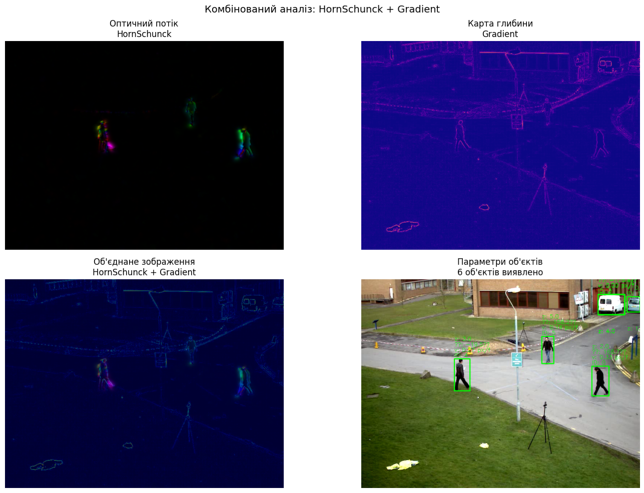
\includegraphics[width=6in,height=4.59207in]{media/image47.png}
\caption{Рис. 4.53 --- HornSchunck\_Gradient}
\end{figure}

На рис. 4.53 наведено результат «HornSchunck\_Gradient», який
використовується для порівняння оптичного потоку, карти глибини та
об'єднаного представлення сцени під час дистанційної ідентифікації
параметрів динамічних об'єктів.

На рис. 4.54 зображено HornSchunck\_MiDaS. Комбінований аналіз:
HornSchunck + MiDaS.

На рис. 4.54 показано результати роботи системи з використанням
класичного глобального алгоритму оптичного потоку Горна--Шунка
(Horn--Schunck) для оцінки руху та нейромережевої моделі MiDaS для
оцінки глибини сцени. Ця комбінація поєднує глобальну гладкість оцінки
руху з універсальністю та хорошою якістю MiDaS.

Ліва панель -- оптичний потік (Horn--Schunck).

Ключові особливості методу Горна--Шунка:

Центральна панель -- карта глибини (MiDaS).

- Чіткі межі об'єктів: перепади глибини на межах об'єктів є добре
помітними.

-- Робастність: MiDaS працює на різноманітних сценах без донавчання
(zero-shot).

Права панель -- об'єднане зображення (Horn--Schunck + MiDaS).

Накладання оптичного потоку Horn--Schunck на карту глибини MiDaS.
Насиченість → інтенсивність руху, яскравість → глибина. Поєднання
глобально гладкого потоку Horn--Schunck з якісною глибиною MiDaS
дозволяє отримати фізично коректну просторову інформацію. Однак основний
недолік Horn--Schunck -- розмиття меж швидко рухомих об'єктів -- не
компенсується навіть якісною глибиною MiDaS, оскільки це властивість
самого методу оптичного потоку.

Детекція об'єктів.

Виявлено 6 об'єктів моделлю DETR. Поєднання з Horn--Schunck + MiDaS
дозволяє обчислити повний набір параметрів (x, y, z, v, θ) з високою
якістю глибини, але з потенційним розмиттям меж у полі оптичного потоку.
Ця комбінація є базовою для порівняння глобальних методів оптичного
потоку з нейромережевими методами оцінки глибини.

\begin{figure}
\centering
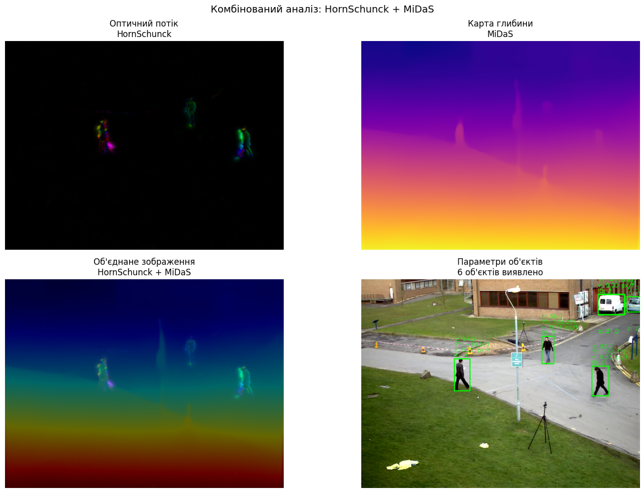
\includegraphics[width=6in,height=4.59207in]{media/image48.png}
\caption{Рис. 4.54 --- HornSchunck\_MiDaS}
\end{figure}

На рис. 4.54 наведено результат «HornSchunck\_MiDaS», який
використовується для порівняння оптичного потоку, карти глибини та
об'єднаного представлення сцени під час дистанційної ідентифікації
параметрів динамічних об'єктів.

\subsubsection{4.4.5 Результати поєднання методу Lucas--Kanade, методів
оцінювання глибини і
трансформерів}\label{ux440ux435ux437ux443ux43bux44cux442ux430ux442ux438-ux43fux43eux454ux434ux43dux430ux43dux43dux44f-ux43cux435ux442ux43eux434ux443-lucaskanade-ux43cux435ux442ux43eux434ux456ux432-ux43eux446ux456ux43dux44eux432ux430ux43dux43dux44f-ux433ux43bux438ux431ux438ux43dux438-ux456-ux442ux440ux430ux43dux441ux444ux43eux440ux43cux435ux440ux456ux432}

На рис. 4.55 зображено LucasKanade\_Bagging. Комбінований аналіз:
LucasKanade + Bagging. На рис. 4.55 показано результати роботи системи з
використанням локального алгоритму оптичного потоку Лукаса--Канаде
(Lucas--Kanade) для оцінки руху та ансамблевого методу бегінгу (Bagging)
для оцінки глибини сцени. Ця комбінація поєднує ефективність локального
методу для вибраних характерних точок з ансамблевим підвищенням
стійкості оцінки глибини. Ліва панель -- оптичний потік (Lucas--Kanade).
Поле оптичного потоку отримане методом Лукаса--Канаде локальним підходом
до оцінки оптичного потоку, який базується на припущенні, що сусідні
пікселі рухаються однаково. Для вікна \(\Omega_{p}\) розміром
\(w\  \times \ w\) розв'язується система рівнянь методом найменших
квадратів:

\(v\  = \ \left( A^{T}A \right)^{- 1}A^{T}b\), (4.3)

\(A^{T}A\  =\)

\(\left\lbrack \Sigma\ I_{x}^{2}\ \ \ \Sigma\ I_{x}I_{y} \right\rbrack\)

\(\left\lbrack \Sigma\ I_{x}I_{y}\ \ \ \Sigma\ I_{y}^{2} \right\rbrack	\)

де \(v\  = \ \lbrack u,\ v\rbrack^{T}\) -- вектор потоку, \(I_{x}\),
\(I_{y}\) -- просторові градієнти, \(I(t)\) -- часова похідна.

Ключові особливості методу Лукаса--Канаде:

-- Локальність: на відміну від глобальних методів (Горна--Шунка), оцінка
виконується лише в областях з достатньою текстурою (де λ1, λ2
\textgreater{} 0).

-- Розріджений потік: метод дає вектори лише для вибраних характерних
точок (кути, текстурні області), що робить його швидким, але неповним.

-- Стійкість до шумів: використання вікна усереднює шум, але розмиває
межі руху.

Кольорове кодування: червоно-жовті тони → рух вправо/вверх, синьо-зелені
→ вліво/вниз; насиченість → інтенсивність руху. На лівій панелі видно,
що вектори присутні лише в текстурних областях (кути будівель, вікна), а
однорідні області (стіни, дорога) не мають оцінки потоку. Центральна
панель -- карта глибини (Bagging). Переваги Bagging: зменшення дисперсії
(локальні шумові викиди згладжуються), підвищення стійкості до аномалій
в окремих кадрах, збереження просторової структури сцени. Кольорова
шкала: теплі тони (жовтий, помаранчевий, червоний) -- ближні об'єкти,
холодні тони (зелений, синій, фіолетовий) -- віддалені. Права панель --
об'єднане зображення (Lucas--Kanade + Bagging). Накладання розрідженого
оптичного потоку Лукаса--Канаде на ансамблеву карту глибини Bagging.
Насиченість → інтенсивність руху, яскравість → глибина. Оскільки метод
Лукаса--Канаде дає вектори лише в текстурних областях, об'єднане
зображення показує рух лише на межах об'єктів, де є достатній градієнт
яскравості. Ансамблева глибина Bagging забезпечує згладжену та фізично
коректну карту, але розрідженість оптичного потоку обмежує загальну
інформативність. Детекція 6 об'єктів моделлю DETR. Поєднання з
Lucas--Kanade + Bagging дозволяє обчислити параметри руху лише для
текстурних областей виявлених об'єктів. Ця комбінація ефективна для
задач, де потрібна швидка оцінка руху характерних точок зі згладженою
ансамблевою глибиною, але непридатна для щільного аналізу руху всієї
сцени.

\begin{figure}
\centering
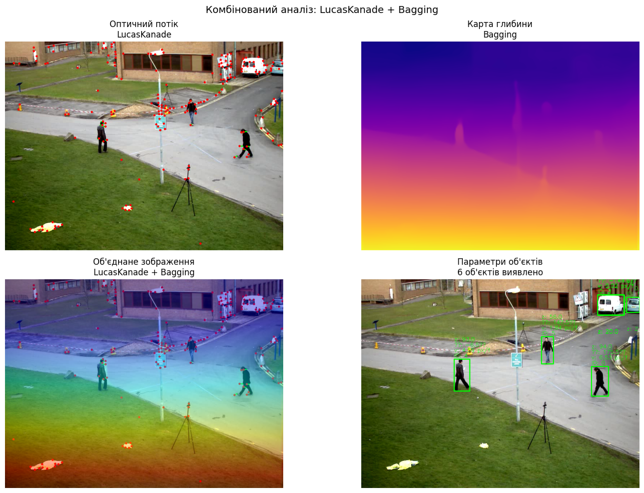
\includegraphics[width=6in,height=4.59207in]{media/image49.png}
\caption{Рис. 4.55 --- LucasKanade\_Bagging}
\end{figure}

На рис. 4.55 наведено результат «LucasKanade\_Bagging», який
використовується для порівняння оптичного потоку, карти глибини та
об'єднаного представлення сцени під час дистанційної ідентифікації
параметрів динамічних об'єктів.

На рис. 4.56 зображено LucasKanade\_Blur. Комбінований аналіз:
LucasKanade + Blur.

На рис. 4.56 показано результати роботи системи з використанням
локального алгоритму оптичного потоку Лукаса--Канаде (Lucas--Kanade) для
оцінки руху та простого методу розмиття (Blur) для оцінки глибини сцени.
Ця комбінація демонструє обмеження локального методу оптичного потоку та
примітивного методу оцінки глибини. Ліва панель -- оптичний потік
(Lucas--Kanade). Центральна панель -- карта глибини (Blur). Оцінка
глибини виконана методом простого розмиття (Blur) -- найпримітивнішим
способом, який не використовує жодної інформації про геометрію сцени.
Основні недоліки методу Blur:

-- Відсутність фізичної коректності: карта глибини є лише згладженою
версією яскравісного каналу зображення.

- Розмиті межі: метод не виділяє межі об'єктів, що унеможливлює точну
сегментацію. Цей метод є «нижньою межею» якості оцінки глибини.

Права панель -- об'єднане зображення (Lucas--Kanade + Blur). Накладання
розрідженого оптичного потоку Лукаса--Канаде на карту глибини Blur.
Насиченість → інтенсивність руху, яскравість → псевдо-глибина. Оскільки
метод Лукаса--Канаде дає вектори лише в текстурних областях, а Blur не
дає фізично коректної глибини, об'єднане зображення має низьку
інформативність: вектори потоку присутні лише на окремих точках, а
фонова глибина не відповідає реальній просторовій структурі сцени.
Детекція 6 об'єктів моделлю DETR. Однак через розрідженість оптичного
потоку та відсутність фізично коректної глибини, визначення повного
набору параметрів (особливо швидкості та просторового положення) є
неможливим. Ця комбінація непридатна для практичного використання в
задачах дистанційної ідентифікації динамічних об'єктів.

\begin{figure}
\centering
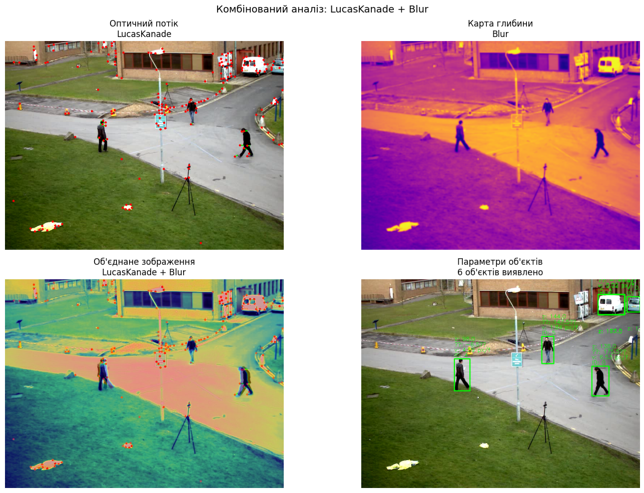
\includegraphics[width=6in,height=4.59207in]{media/image50.png}
\caption{Рис. 4.56 --- LucasKanade\_Blur}
\end{figure}

На рис. 4.56 наведено результат «LucasKanade\_Blur», який
використовується для порівняння оптичного потоку, карти глибини та
об'єднаного представлення сцени під час дистанційної ідентифікації
параметрів динамічних об'єктів.

На рис. 4.57 зображено LucasKanade\_Boosting. Комбінований аналіз:
LucasKanade + Boosting.

На рис. 4.57 показано результати роботи системи з використанням
локального алгоритму оптичного потоку Лукаса--Канаде (Lucas--Kanade) для
оцінки руху та ансамблевого методу бустінгу (Boosting) для оцінки
глибини сцени. Ця комбінація поєднує ефективність локального методу для
вибраних характерних точок з ансамблевим підвищенням точності та
підкресленням меж об'єктів. Ліва панель -- оптичний потік
(Lucas--Kanade). Центральна панель -- карта глибини (Boosting).

\[D_{boost} = \ \Sigma(m = 1..M)\alpha_{m}D^{m},\ \alpha_{m} = \frac{1}{2}\ln\left( \frac{1\  - \ \varepsilon_{m}}{\varepsilon_{m}} \right)\]

де \(\alpha_{m}\) -- вага, обернено пропорційна помилці
\(\varepsilon_{m}\).

Права панель -- об'єднане зображення (Lucas--Kanade + Boosting).
Накладання розрідженого оптичного потоку Лукаса--Канаде на карту глибини
Boosting. Насиченість → інтенсивність руху, яскравість → глибина.
Оскільки метод Лукаса--Канаде дає вектори лише в текстурних областях,
об'єднане зображення показує рух лише на межах об'єктів, де є достатній
градієнт яскравості. Ансамблева глибина Boosting забезпечує підкреслені
межі та фізично коректну карту, але розрідженість оптичного потоку
обмежує загальну інформативність. Бустінг частково компенсує відсутність
інформації про рух в однорідних областях, оскільки підкреслює межі, де
метод Лукаса--Канаде все ще може надати оцінку. Детекція 6 об'єктів
моделлю DETR. Поєднання з Lucas--Kanade + Boosting дозволяє обчислити
параметри руху лише для текстурних областей виявлених об'єктів, але з
підвищеною точністю на межах завдяки Boosting. Ця комбінація ефективна
для задач, де потрібна швидка оцінка руху характерних точок з
підкресленими межами глибини, але непридатна для щільного аналізу руху
всієї сцени.

\begin{figure}
\centering
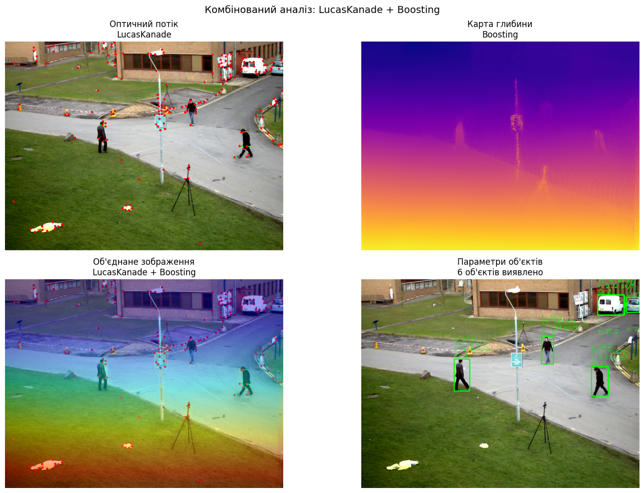
\includegraphics[width=6in,height=4.59207in]{media/image51.png}
\caption{Рис. 4.57 --- LucasKanade\_Boosting}
\end{figure}

На рис. 4.57 наведено результат «LucasKanade\_Boosting», який
використовується для порівняння оптичного потоку, карти глибини та
об'єднаного представлення сцени під час дистанційної ідентифікації
параметрів динамічних об'єктів.

На рис. 4.58 зображено LucasKanade\_DPT\_Large. Комбінований аналіз:
LucasKanade + DPT\_Large.

На рис. 4.58 показано результати роботи системи з використанням
локального алгоритму оптичного потоку Лукаса--Канаде (Lucas--Kanade) для
оцінки руху та трансформерної моделі DPT\_Large для оцінки глибини
сцени. Ця комбінація поєднує ефективність локального методу для вибраних
характерних точок з високою роздільною здатністю та чіткими межами
DPT\_Large.

Ліва панель -- оптичний потік (Lucas--Kanade). Центральна панель --
карта глибини (DPT\_Large). Права панель -- об'єднане зображення
(Lucas--Kanade + DPT\_Large).

Накладання розрідженого оптичного потоку Лукаса--Канаде на
високороздільну карту глибини DPT\_Large. Насиченість → інтенсивність
руху, яскравість → глибина. Оскільки метод Лукаса--Канаде дає вектори
лише в текстурних областях, об'єднане зображення показує рух лише на
межах об'єктів, де є достатній градієнт яскравості. Високороздільна
глибина DPT\_Large забезпечує детальну просторову інформацію, але
розрідженість оптичного потоку обмежує загальну інформативність. На
відміну від методу Горна--Шунка, Lucas--Kanade не страждає від розмиття
меж, але потребує наявності текстурних областей для обчислення потоку.
Детекція 6 об'єктів моделлю DETR. Поєднання з Lucas--Kanade + DPT\_Large
дозволяє обчислити параметри руху лише для текстурних областей виявлених
об'єктів. Ця комбінація ефективна для задач, де потрібна швидка оцінка
руху характерних точок з високоякісною деталізованою глибиною, але
непридатна для щільного аналізу руху всієї сцени.

\begin{figure}
\centering
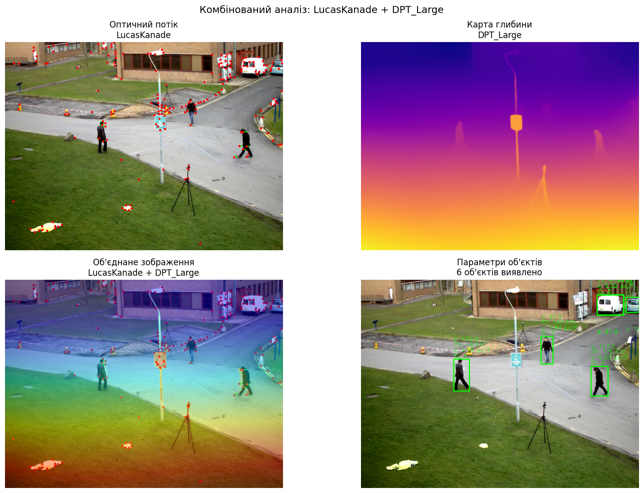
\includegraphics[width=6in,height=4.59565in]{media/image52.png}
\caption{Рис. 4.58 --- LucasKanade\_DPT\_Large}
\end{figure}

На рис. 4.58 наведено результат «LucasKanade\_DPT\_Large», який
використовується для порівняння оптичного потоку, карти глибини та
об'єднаного представлення сцени під час дистанційної ідентифікації
параметрів динамічних об'єктів.

На рис. 4.59 зображено LucasKanade\_GeoNet. Комбінований аналіз:
LucasKanade + GeoNet.

На рис. 4.59 показано результати роботи системи з використанням
локального алгоритму оптичного потоку Лукаса--Канаде (Lucas--Kanade) для
оцінки руху та інтегрованої моделі GeoNet для оцінки глибини сцени. Ця
комбінація поєднує ефективність локального методу для вибраних
характерних точок з просторово-часовою узгодженістю GeoNet. Центральна
панель -- карта глибини (GeoNet). Оцінка глибини виконана моделлю GeoNet
-- глибокою нейронною архітектурою, яка поєднує задачу оцінки глибини
(DepthNet), пози камери (PoseNet) та оптичного потоку (ResFlowNet) в
єдиній неконтрольованій (unsupervised) структурі. Ключові особливості
GeoNet:

-- Спільне навчання: одночасне навчання оцінки глибини, пози та
оптичного потоку.

-- Фотометрична узгодженість: функція втрат базується на реконструкції
кадрів.

-- Геометрична коректність: карта глибини є фізично правдоподібною.

Права панель -- об'єднане зображення (Lucas--Kanade + GeoNet).

Накладання розрідженого оптичного потоку Лукаса--Канаде на карту глибини
GeoNet. Насиченість → інтенсивність руху, яскравість → глибина. Оскільки
метод Лукаса--Канаде дає вектори лише в текстурних областях, об'єднане
зображення показує рух лише на межах об'єктів, де є достатній градієнт
яскравості. Узгоджена глибина GeoNet забезпечує фізично коректну
просторову інформацію, але розрідженість оптичного потоку обмежує
загальну інформативність. На відміну від методу Горна--Шунка,
Lucas--Kanade не страждає від розмиття меж, але потребує наявності
текстурних областей для обчислення потоку. Детекція об'єктів. Виявлено 6
об'єктів моделлю DETR. Поєднання з Lucas--Kanade + GeoNet дозволяє
обчислити параметри руху лише для текстурних областей виявлених
об'єктів. Ця комбінація ефективна для задач, де потрібна швидка оцінка
руху характерних точок з узгодженою глибиною, особливо в сценах з
рухомою камерою, але непридатна для щільного аналізу руху всієї сцени.

\begin{figure}
\centering
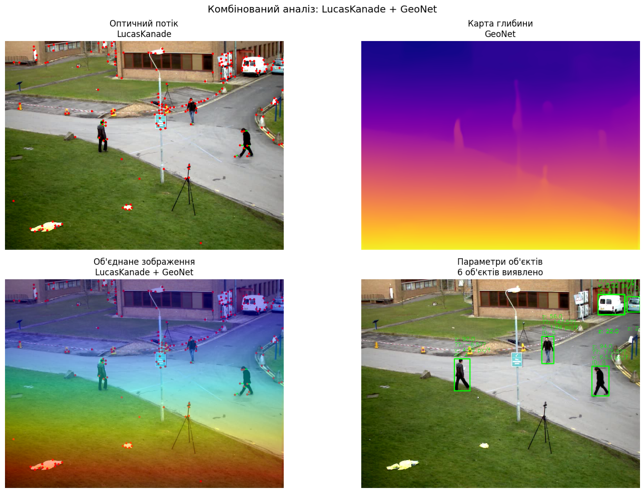
\includegraphics[width=6in,height=4.59207in]{media/image53.png}
\caption{Рис. 4.59 --- LucasKanade\_GeoNet}
\end{figure}

На рис. 4.59 наведено результат «LucasKanade\_GeoNet», який
використовується для порівняння оптичного потоку, карти глибини та
об'єднаного представлення сцени під час дистанційної ідентифікації
параметрів динамічних об'єктів.

На рис. 4.60 зображено LucasKanade\_Gradient. Комбінований аналіз:
LucasKanade + Gradient.

На рис. 4.60 показано результати роботи системи з використанням
локального алгоритму оптичного потоку Лукаса--Канаде (Lucas--Kanade) для
оцінки руху та методу градієнта (Gradient) для оцінки глибини сцени. Ця
комбінація демонструє можливості використання градієнтних методів для
виділення меж об'єктів при локальній оцінці оптичного потоку. Центральна
панель -- карта глибини (Gradient). Особливості методу Gradient:

Права панель -- об'єднане зображення (Lucas--Kanade + Gradient).
Накладання розрідженого оптичного потоку Лукаса--Канаде на градієнтну
карту. Насиченість → інтенсивність руху, яскравість → градієнт. Оскільки
обидва методи (Lucas--Kanade та Gradient) працюють лише в областях з
високим градієнтом (кути, межі), об'єднане зображення показує рух саме
на контурах об'єктів. Вектори потоку чітко видно на межах, де є достатня
текстурна інформація. Ця комбінація може бути корисною для аналізу руху
меж об'єктів, але не дає інформації про рух внутрішніх областей та
абсолютні значення глибини. Детекція 6 об'єктів моделлю DETR. Однак
через розрідженість оптичного потоку та відсутність абсолютних значень
глибини, визначення повного набору параметрів (особливо швидкості та
просторового положення) є обмеженим. Ця комбінація може бути корисною
лише для задач, де потрібно проаналізувати рух меж об'єктів, але не для
кількісної оцінки параметрів динамічних об'єктів.

\begin{figure}
\centering
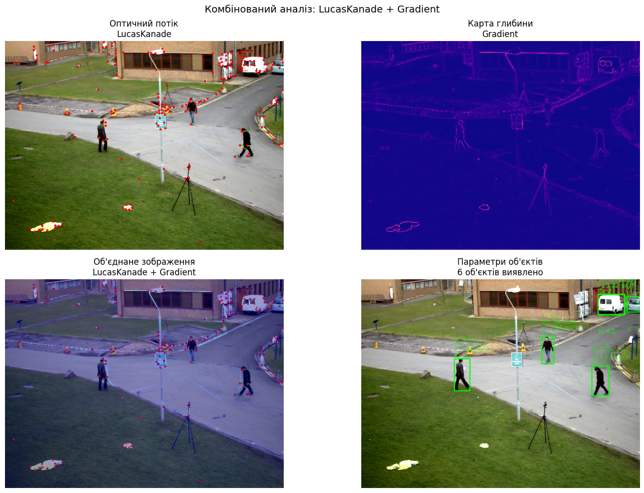
\includegraphics[width=6in,height=4.59207in]{media/image54.png}
\caption{Рис. 4.60 --- LucasKanade\_Gradient}
\end{figure}

На рис. 4.60 наведено результат «LucasKanade\_Gradient», який
використовується для порівняння оптичного потоку, карти глибини та
об'єднаного представлення сцени під час дистанційної ідентифікації
параметрів динамічних об'єктів.

На рис. 4.61 зображено LucasKanade\_MiDaS. Комбінований аналіз:
LucasKanade + MiDaS.

На рис. 4.61 показано результати роботи системи з використанням
локального алгоритму оптичного потоку Лукаса--Канаде (Lucas--Kanade) для
оцінки руху та нейромережевої моделі MiDaS для оцінки глибини сцени. Ця
комбінація поєднує ефективність локального методу для вибраних
характерних точок з універсальністю та хорошою якістю MiDaS.

Центральна панель -- карта глибини (MiDaS).

- Чіткі межі об'єктів: перепади глибини на межах об'єктів є добре
помітними.

-- Робастність: MiDaS працює на різноманітних сценах без донавчання
(zero-shot).

Права панель -- об'єднане зображення (Lucas--Kanade + MiDaS).

Накладання розрідженого оптичного потоку Лукаса--Канаде на карту глибини
MiDaS. Насиченість → інтенсивність руху, яскравість → глибина. Оскільки
метод Лукаса--Канаде дає вектори лише в текстурних областях, об'єднане
зображення показує рух лише на межах об'єктів, де є достатній градієнт
яскравості. Якісна глибина MiDaS забезпечує фізично коректну просторову
інформацію, але розрідженість оптичного потоку обмежує загальну
інформативність. На відміну від методу Горна--Шунка, Lucas--Kanade не
страждає від розмиття меж, але потребує наявності текстурних областей
для обчислення потоку. Детекція 6 об'єктів моделлю DETR. Поєднання з
Lucas--Kanade + MiDaS дозволяє обчислити параметри руху лише для
текстурних областей виявлених об'єктів. Ця комбінація є базовою для
порівняння локальних методів оптичного потоку з нейромережевими методами
оцінки глибини, але непридатна для щільного аналізу руху всієї сцени.

\begin{figure}
\centering
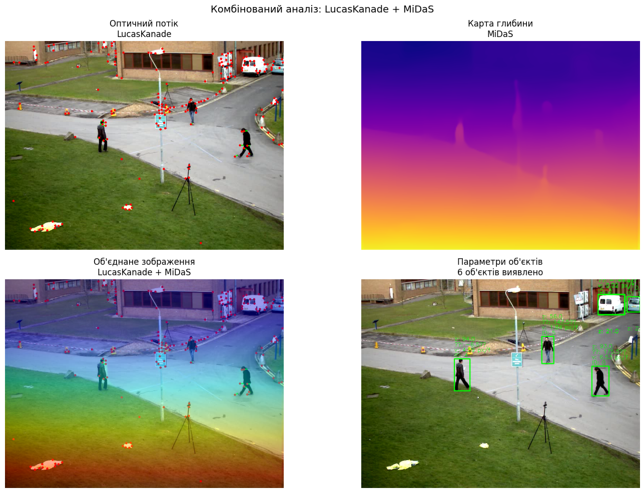
\includegraphics[width=6in,height=4.59207in]{media/image55.png}
\caption{Рис. 4.61 --- LucasKanade\_MiDaS}
\end{figure}

На рис. 4.61 наведено результат «LucasKanade\_MiDaS», який
використовується для порівняння оптичного потоку, карти глибини та
об'єднаного представлення сцени під час дистанційної ідентифікації
параметрів динамічних об'єктів.

\subsection{4. Реалізація методів ідентифікації на основі глибокого
навчання}\label{ux440ux435ux430ux43bux456ux437ux430ux446ux456ux44f-ux43cux435ux442ux43eux434ux456ux432-ux456ux434ux435ux43dux442ux438ux444ux456ux43aux430ux446ux456ux457-ux43dux430-ux43eux441ux43dux43eux432ux456-ux433ux43bux438ux431ux43eux43aux43eux433ux43e-ux43dux430ux432ux447ux430ux43dux43dux44f}

У підрозділі «4.5 Реалізація методів ідентифікації на основі глибокого
навчання» для подальшого викладу використано такі формульні залежності:
(4.12).

У підрозділі «4.5 Реалізація методів ідентифікації на основі глибокого
навчання» для подальшого викладу використано такі формульні залежності:
(4.13).

У підрозділі «4.5 Реалізація методів ідентифікації на основі глибокого
навчання» для подальшого викладу використано такі формульні залежності:
(4.14).

У підрозділі «4.5 Реалізація методів ідентифікації на основі глибокого
навчання» для подальшого викладу використано такі формульні залежності:
(4.15).

Опис додаткової розробленої моделі з використанням GeoNet. Реалізована
інтеграція GeoNet для обробки відео шляхом оцінювання глибини зображень
(monocular depth estimation), що дає змогу визначати один із
найважливіших параметрів об'єкта -- відстань до елементів сцени.

GeoNet працює із відеофреймами, які попередньо витягуються з відео,
зберігаються у вигляді зображень та форматуються для подальшої обробки.
Входи обробляються через GeoNet, що передбачає отримання параметрів.

Етап підготовки даних. GeoNet здійснює попередню обробку кадрів відео з
використанням скрипта. Цей етап включає зміну розмірів зображень,
створення необхідних послідовностей кадрів (наприклад, для аналізу
оптичного потоку або оцінки глибини) і видалення статичних об'єктів для
покращення результатів.

Інференс. Основний обчислювальний етап виконується за допомогою
geonet\_main.py, який аналізує дані та генерує результати, такі як
глибинні карти, оптичний потік або оцінки позиції. Для цього
використовуються попередньо натреновані моделі, збережені у вигляді
контрольних точок (checkpoints).

Вивід результатів. Глибинні карти (depth maps) зберігаються у
визначеному каталозі та візуалізуються для оцінки результатів роботи
моделі{[}\hyperref[_Ref221389746]{64}{]}.

На рис. 4.62 показано реалізовану модель з використанням
GeoNet.\hyperref[_Ref221383624]{Рис. 4.62 -- а) модель, що планувалась;
б) реалізована модель з використанням GeoNet}

\protect\phantomsection\label{_Ref221383624}{}Рис. 4.62 --реалізована
модель з використанням GeoNet

На рис. 4.63 показано загальну модель з використанням GeoNet, яка працює
паралельно з DETR та модулем оптичного
потоку.\hyperref[_Ref221383821]{Рис. 4.63 -- Загальна реалізована модель
з використанням GeoNet}

\protect\phantomsection\label{_Ref221383821}{}Рис. 4.63 -- Загальна
реалізована модель з використанням GeoNet

Оцінка глибини (Depth Estimation). Результати роботи GeoNet
продемонстрували можливість точного визначення глибини на основі кадрів
відео. Згенеровані глибинні карти надають детальну інформацію про
структуру сцени, що корисно для відстеження об'єктів у просторі та
побудови 3D-моделей 51; 54; 55.

Мета оцінки глибини полягає в обчисленні карти глибини D ∈ ℝ\^{}H×W із
заданого 2D-зображення I ∈ ℝ\^{}H×W×3 за формулою (4.1), де кожне
значення глибини d\_i,j ∈ D представляє фізичну відстань між пікселем
i\_i,j ∈ I та камерою.

\(D:R^{H \times W}\text{з}I:R^{H \times W \times 3}\) (4.1)

Нехай M -- кількість пікселів у зображенні з дійсними значеннями
глибини, θ -- параметри моделі. Нехай d = d(θ) ∈ ℝ\^{}M -- передбачена
диспаратність, а d* ∈ ℝ\^{}M -- відповідна правдива диспаратність;
функцію втрат визначено формулою (4.2).

\(L_{ssi}\left( \widehat{d},{\widehat{d}}^{*} \right) = \frac{1}{2M}\sum_{i = 1}^{M}{\rho\left( {\widehat{d}}_{i} - {\widehat{d}}_{i}^{*} \right)}\)
(4.2)

де d̂ і d̂\^{}* --- масштабовані та зсунуті версії передбачень і правдивої
глибини, а ρ визначає конкретний тип функції втрат.

Вирівнювання на основі найменших квадратів виконується за формулами
(4.3), (4.4):

\((S,t) = \backslash arg\min_{s,t}\sum_{i = 1}^{M}{(sd_{i} + t - d_{i}^{*})^{2}}\)
(4.3)

\(H^{opt} = \left( {\sum_{i = 1}^{M}{{\widetilde{d}}_{i}{\widetilde{d}}_{i}^{\top}}} \right)^{- 1}\left( {\sum_{i = 1}^{M}{{\widetilde{d}}_{i}d_{i}^{*}}} \right)\)
(4.4)

де \(ilded_{i} = \ \left( d_{i},\ 1 \right)^{op}\),
\(h\  = \ (s,\ t)^{op}\)

Робастне вирівнювання на основі медіани задається формулами (4.5),
(4.6):

\(T(d) = \text{median}(d),s(d) = \frac{1}{M}\sum_{i = 1}^{M}\left| d_{i} - t(d) \right|\)
(4.5)

\(\widehat{D} = \frac{d - t(d)}{s(d)},{\widehat{d}}^{*} = \frac{d^{*} - t\left( d^{*} \right)}{s\left( d^{*} \right)}\)
(4.6)

Тримована втрата (Trimmed Loss) обчислюється за формулою (4.7):

\(L_{ssitrim}\left( \widehat{d},{\widehat{d}}^{*} \right) = \frac{1}{2M}\sum_{j = 1}^{U_{m}}{\rho_{mae}\left( {\widehat{d}}_{j} - {\widehat{d}}_{j}^{*} \right)}\)
(4.7)

де
\(\left| {\widehat{d}}_{j}–\ {\widehat{d}}_{j}^{*} \right| \leq \ \left| {\widehat{d}}_{j} + 1\ –\ {\widehat{d}}_{j} + 1^{*} \right|\),
\(U_{m} = \ 0.8M\) (відкидання 20\% найбільших залишків)

Градієнтний регуляризатор задається формулою (4.8):

\(L_{reg}\left( \widehat{d},{\widehat{d}}^{*} \right) = \frac{1}{M}\sum_{k = 1}^{K}{\sum_{i = 1}^{M}\left( {\left| \nabla_{x}R_{i}^{k} \right| + \left| \nabla_{y}R_{i}^{k} \right|} \right)}\)
(4.8)

де \(R_{i} = \ {\widehat{d}}_{i}–\ {\widehat{d}}_{i}^{*}\), а \(R^{k}\)
позначає різницю карт диспаратності на масштабі \(k\) (K=4 рівні)

Повна функція втрат визначається формулою (4.9):

\(L_{l} = \frac{1}{N_{l}}\sum_{n = 1}^{N_{l}}\left( {L_{ssi}({\widehat{d}}^{n},({\widehat{d}}^{*})^{n}) + \alpha L_{reg}({\widehat{d}}^{n},({\widehat{d}}^{*})^{n})} \right)\)
(4.9)

де \(\alpha\  = \ 0.5\), \(N_{l}\) --- розмір навчального набору

Наївне змішування та принципове змішування даних для багатонаборного
навчання формалізовано у формулі (4.10). Наївне змішування передбачає
вибірку B/L зразків з кожного набору даних у міні-пакеті розміру B, де
\(L\) -- кількість наборів даних; принципове змішування розглядає
навчання на кожному наборі як окреме завдання і шукає наближений
Парето-оптимум.

\({Min}_{\theta}\left( {L_{1}(\theta),\ldots,L_{L}(\theta)} \right)^{\top}\)
(4.10)

Декодер збирає набір токенів у виглядові представлення ознак на різних
роздільностях. Операція Reassemble для відновлення виглядових
представлень з вихідних токенів трансформерного кодера описується
формулами (4.11)--(4.16):

\(\text{Reassemble}_{s}^{\widehat{D}}(t) = \left( \text{Resample}_{s} \circ \text{Concatenate} \circ \text{Read} \right)(t)\)
(4.11)

де s позначає співвідношення вихідного розміру відновленого
представлення відносно вхідного зображення, а D̂ --- вихідну розмірність
ознак.

\(\text{Read}_{ignore}(t) = \left\{ t_{1},\ldots,t_{N_{p}} \right\}\)
(4.12)

\(\text{Read}_{add}(t) = \left\{ t_{1} + t_{0},\ldots,t_{N_{p}} + t_{0} \right\}\)
(4.13)

\(\text{Read}_{proj}(t) = \left\{ \text{mlp}\left( \text{cat}\left( t_{1},t_{0} \right) \right),\ldots,\text{mlp}\left( \text{cat}\left( t_{N_{p}},t_{0} \right) \right) \right\}\)
(4.14)

\(\text{Concatenate}:R^{N_{p} \times D} \rightarrow R^{\frac{H}{p} \times \frac{W}{p} \times D}\)
(4.15)

\(\text{Resample}_{s}:R^{\frac{H}{p} \times \frac{W}{p} \times D} \rightarrow R^{\frac{H}{s} \times \frac{W}{s} \times \widehat{D}}\)
(4.16)

\subsection{4. Тестування інформаційної
технології}\label{ux442ux435ux441ux442ux443ux432ux430ux43dux43dux44f-ux456ux43dux444ux43eux440ux43cux430ux446ux456ux439ux43dux43eux457-ux442ux435ux445ux43dux43eux43bux43eux433ux456ux457}

Для кількісного оцінювання якості ідентифікації параметрів динамічних
об'єктів у розробленій інформаційній технології застосовується система
метрик, яка включає показники для оцінки точності оптичного потоку,
глибини та якості сегментації. Далі розглянуто основні метрики, що
використовуються для оцінювання ефективності запропонованих методів.
Середня кінцева похибка (EPE, End-Point Error) є фундаментальною
метрикою для оцінки точності оптичного потоку. Вона характеризує середню
евклідову відстань між передбаченим та істинним векторами руху для всіх
пікселів зображення:

\(EPE = \frac{1}{N}\sum_{i = 1}^{N}\sqrt{\left( u_{i} - u_{i}^{qt} \right)^{2} + \left( v_{i} - v_{i}^{qt} \right)^{2}}\)
(4.17)

де N -- загальна кількість пікселів у зображенні; \(u_{i}\), \(v_{i}\)
-- горизонтальна та вертикальна компоненти передбаченого вектора
оптичного потоку для i-го пікселя; \(u_{i}^{gt}\), \(v_{i}^{gt}\) --
відповідні компоненти істинного (еталонного) вектора оптичного потоку.
Ця метрика безпосередньо вимірює похибку визначення переміщення кожного
пікселя в пікселях. Чим менше значення EPE, тим вища точність оцінки
руху. Значення EPE менше 1 пікселя вважається відмінним результатом,
оскільки це означає, що середнє відхилення передбаченого положення
пікселя від істинного не перевищує розміру одного пікселя.

Середня кутова похибка AAE (Angular Average Error) вимірює розбіжність
між передбаченим та істинним векторами руху за напрямком і визначається
за формулою (4.18):

\(AAE = \frac{1}{N}\sum_{i = 1}^{N}{arccos\left( \frac{u_{i}u_{i}^{qt} + v_{i}v_{i}^{qt} + 1}{\sqrt{u_{i}^{2} + v_{i}^{2} + 1} \cdot \sqrt{\left( u_{i}^{qt} \right)^{2} + \left( v_{i}^{qt} \right)^{2} + 1}} \right)}\)
(4.18)

Додавання одиниці в чисельнику та знаменнику забезпечує коректне
обчислення кута навіть для нульових векторів. Ця метрика є особливо
важливою в задачах, де критичним є не тільки модуль швидкості, але й
траєкторія руху об'єкта. Значення AAE вимірюються в радіанах: чим ближче
значення до нуля, тим точніше визначено напрямок руху. Значення AAE
менше 0.1 радіана (приблизно 5.7 градуса) свідчить про високу точність
орієнтації векторів руху.

Середньоквадратична похибка RMSE (Root Mean Square Error) є стандартною
метрикою для оцінки точності відновлення глибини сцени та обчислюється
за формулою (4.19):

\(RMSE = \sqrt{\frac{1}{N}\sum_{i = 1}^{N}\left( D_{i} - D_{i}^{qt} \right)^{2}}\)
(4.19)

де \(D_{i}\) -- передбачена глибина (відстань від камери до об'єкта) для
\(i\)-го пікселя; \(D_{i}^{gt}\) -- істинне значення глибини. Головною
особливістю RMSE є піднесення похибки до квадрату перед підсумовуванням,
що робить цю метрику особливо чутливою до великих похибок (викидів).
Якщо модель робить декілька грубих помилок у визначенні глибини,
значення RMSE значно зростатиме, що дозволяє виявити нестабільність
алгоритму. На практиці значення RMSE менше 10 умовних одиниць глибини
вказує на хорошу якість відновлення.

Середня абсолютна похибка MAE (Mean Absolute Error) є альтернативною
метрикою для оцінки точності глибини та визначається за формулою (4.20):

\(MAE = \frac{1}{N}\sum_{i = 1}^{N}\left| D_{i} - D_{i}^{qt} \right|\)
(4.20)

На відміну від RMSE, MAE використовує абсолютне значення похибки без
піднесення до квадрату. Це робить MAE більш стійкою до викидів і дає
змогу отримати більш інтерпретовану оцінку -- середню абсолютну похибку
визначення глибини в тих самих одиницях, що й самі дані. Наприклад, якщо
MAE = 5 одиниць, це означає, що в середньому модель помиляється у
визначенні глибини на 5 одиниць. MAE є більш репрезентативною метрикою
для практичних застосувань, оскільки вона безпосередньо вказує на типову
величину помилки.

Пікове відношення сигнал/шум PSNR (Peak Signal-to-Noise Ratio)
використовується для оцінки якості відновлення карти глибини як
зображення та визначається за формулою (4.21):

\(PSNR = 10\log_{10}\left( \frac{{MAX}^{2}}{MSE} \right)\) (4.21)

де MAX -- максимальне можливе значення глибини (255 для 8-бітних
зображень), а MSE -- середньоквадратична похибка, що обчислюється за
формулою (4.22):

\(MSE = \frac{1}{N}\sum_{i = 1}^{N}\left( D_{i} - D_{i}^{qt} \right)^{2}\)
(4.22)

PSNR вимірюється в децибелах (дБ) і є логарифмічною мірою відношення
максимально можливої потужності сигналу до потужності шуму, що спотворює
сигнал. Інтерпретація PSNR є наступною: чим вище значення, тим менші
спотворення вносить алгоритм. Значення PSNR вище 30 дБ свідчить про
високу якість відновлення глибинної карти, при цьому спотворення
практично непомітні для подальших алгоритмів аналізу. Значення PSNR вище
40 дБ вважається відмінним, оскільки відповідає майже ідеальному
відновленню.

Intersection over Union (IoU) є стандартною метрикою для оцінки точності
сегментації об'єктів у комп'ютерному зорі та задається формулою (4.23):

\(IoU = \frac{TP}{TP + FP + FN}\) (4.23)

де TP (True Positive) -- кількість пікселів, правильно віднесених до
об'єкта (істинно позитивні); FP (False Positive) -- кількість пікселів,
хибно віднесених до об'єкта (хибно позитивні, помилкові спрацювання); FN
(False Negative) -- кількість пікселів об'єкта, які модель пропустила
(хибно негативні). Геометричний зміст IoU -- це відношення площі
перетину передбаченої та істинної масок об'єкта до площі їх об'єднання.
IoU приймає значення від 0 (повна невідповідність) до 1 (ідеальний
збіг). У практичних задачах значення IoU вище 0.7 вважається хорошим
результатом, вище 0.8 -- дуже хорошим, а вище 0.9 -- відмінним.

Коефіцієнт Дайса (Dice) є альтернативною метрикою якості сегментації,
тісно пов'язаною з IoU, і визначається за формулою (4.24):

\(Dice = \frac{2TP}{2TP + FP + FN}\) (4.24)

Коефіцієнт Дайса, також відомий як F1-міра, обчислює зважене відношення
спільних елементів до суми елементів обох множин. На відміну від IoU,
Dice надає вдвічі більшу вагу спільним елементам; зв'язок між цими
метриками подано у формулі (4.25). Значення Dice вище 0.8 свідчить про
високу якість сегментації, а вище 0.9 -- про відмінну.

Аналіз результатів. У результаті виконання обробки відео з використанням
DETR, модель успішно виявляє об'єкти на кожному кадрі, і середній час
обробки для одного кадру може бути виміряний, що дозволяє оцінити
ефективність моделі.

В обчисленні оптичного потоку за допомогою методу Farneback на основі
двох послідовних кадрів отримано точні дані про напрямок та швидкість
руху об'єктів, що дозволяє покращити відстеження візуальних змін у
кадрі.

Для кожного кадру відео вимірюється час обробки для детекції об'єктів та
для обчислення оптичного потоку, що дозволяє оцінити ефективність
кожного етапу обробки та оптимізувати продуктивність системи.

Інтеграція з іншими методами. В поєднанні з моделлю DETR результати
глибинних карт використані для покращення розпізнавання об'єктів, а
також для визначення їх положення та руху в просторі, що робить систему
потужним інструментом для аналізу відеопотоків.

Для покращення реалізованої моделі та майбутнього представлення у
вигляді цілісної системи доцільним є використання методів бустінгу та
бегінгу. Бустінг дозволяє послідовно комбінувати кілька моделей, кожна з
яких коригує помилки попередньої, що забезпечує високу точність
виявлення та відстеження об'єктів. Застосування цього підходу може
значно покращити продуктивність системи в умовах складних середовищ,
таких як зміна освітлення або перекриття об'єктів. У поєднанні з DETR та
оптичним потоком бустінг здатний підвищити ефективність аналізу
динамічних об'єктів у відеопотоках.

Бегінг, у свою чергу, забезпечує зниження варіативності моделей шляхом
паралельного навчання декількох базових моделей на різних підмножинах
даних. Це сприяє підвищенню стійкості системи до шумів у вхідних даних
та підвищує загальну надійність. Інтеграція цих підходів із
застосуванням мета-алгоритму дозволяє створити ансамбль, який об'єднує
результати всіх компонентів у єдину систему. Така архітектура
забезпечить оптимальну взаємодію між DETR, GeoNet, оптичним потоком та
іншими компонентами, що значно покращить ефективність і адаптивність
системи в реальних сценаріях {[}\hyperref[_Ref221384139]{56}{]}.

Експериментальні дослідження ефективності розробленої інформаційної
технології були спрямовані на верифікацію точності, надійності та
узгодженості модулів детекції, оптичного потоку й оцінювання глибини.
Програмний експеримент виконано на тестовому відеопотоці vtest.avi;
склад використаних моделей, референсних оцінок і доступність зовнішніх
компонентів наведено в табл. 4.2.

\begin{longtable}[]{@{}
  >{\raggedright\arraybackslash}p{(\linewidth - 2\tabcolsep) * \real{0.3739}}
  >{\raggedright\arraybackslash}p{(\linewidth - 2\tabcolsep) * \real{0.6071}}@{}}
\caption{\protect\phantomsection\label{_Ref226482723}{}Таблиця 4.2 --
Умови та склад програмного експерименту}\tabularnewline
\toprule\noalign{}
\begin{minipage}[b]{\linewidth}\raggedright
\textbf{Параметр}
\end{minipage} & \begin{minipage}[b]{\linewidth}\raggedright
\textbf{Значення}
\end{minipage} \\
\midrule\noalign{}
\endfirsthead
\toprule\noalign{}
\begin{minipage}[b]{\linewidth}\raggedright
\textbf{Параметр}
\end{minipage} & \begin{minipage}[b]{\linewidth}\raggedright
\textbf{Значення}
\end{minipage} \\
\midrule\noalign{}
\endhead
\bottomrule\noalign{}
\endlastfoot
Відеодані & vtest.avi з набору прикладів OpenCV; використано два
послідовні кадри \\
Середовище виконання & CPU; завантаження DETR і MiDaS виконано з кешу
моделей \\
Детектор об'єктів & DETR facebook/detr-resnet-50; YOLO у цьому запуску
недоступний \\
Методи оптичного потоку & Farneback, Lucas--Kanade, Horn--Schunck,
FlowNet-проксі, GeoNet-проксі \\
Методи оцінювання глибини & Blur, Gradient, MiDaS, DPT\_Large,
GeoNet-проксі, Bagging, Boosting \\
Референсні оцінки & flow\_gt = Farneback; depth\_gt = MiDaS, тому
частина метрик є відносною \\
Вихідні результати & 35 комбінацій методів; 6 об'єктів, виявлених DETR з
довірою 0,74--1,00 \\
\end{longtable}

Для уточнення експериментальної частини програмна реалізація була
перевірена на тестовому відеопотоці vtest.avi з бібліотеки OpenCV.
Обчислення виконувались на CPU; для детекції використано DETR, для
оцінювання глибини -- MiDaS, DPT\_Large, GeoNet-проксі, Blur, Gradient
та ансамблеві варіанти Bagging і Boosting, а для оптичного потоку --
Farneback, Lucas--Kanade, Horn--Schunck, FlowNet-проксі та
GeoNet-проксі. У цьому запуску YOLO не був доступний, а FlowNet/RAFT
також не завантажився, тому для відповідних конфігурацій застосовано
резервний розрахунок на основі Farneback. Це обмеження враховано під час
інтерпретації результатів.

За результатами запуску DETR на другому кадрі відеопослідовності
виявлено шість об'єктів. Розраховані координати, відносна глибина,
швидкість і напрямок руху наведено в табл. 4.3.

\begin{longtable}[]{@{}
  >{\raggedright\arraybackslash}p{(\linewidth - 12\tabcolsep) * \real{0.1293}}
  >{\raggedright\arraybackslash}p{(\linewidth - 12\tabcolsep) * \real{0.1435}}
  >{\raggedright\arraybackslash}p{(\linewidth - 12\tabcolsep) * \real{0.1391}}
  >{\raggedright\arraybackslash}p{(\linewidth - 12\tabcolsep) * \real{0.1474}}
  >{\raggedright\arraybackslash}p{(\linewidth - 12\tabcolsep) * \real{0.1375}}
  >{\raggedright\arraybackslash}p{(\linewidth - 12\tabcolsep) * \real{0.1593}}
  >{\raggedright\arraybackslash}p{(\linewidth - 12\tabcolsep) * \real{0.1439}}@{}}
\caption{Таблиця 4.3 -- Параметри динамічних об'єктів, виявлених DETR у
тестовому відеопотоці}\tabularnewline
\toprule\noalign{}
\begin{minipage}[b]{\linewidth}\raggedright
\textbf{ID}
\end{minipage} & \begin{minipage}[b]{\linewidth}\raggedright
\textbf{Клас}
\end{minipage} & \begin{minipage}[b]{\linewidth}\raggedright
\textbf{Довіра}
\end{minipage} & \begin{minipage}[b]{\linewidth}\raggedright
\textbf{x; y, пікс.}
\end{minipage} & \begin{minipage}[b]{\linewidth}\raggedright
\textbf{z}
\end{minipage} & \begin{minipage}[b]{\linewidth}\raggedright
\textbf{v, px/кадр}
\end{minipage} & \begin{minipage}[b]{\linewidth}\raggedright
\textbf{θ, град}
\end{minipage} \\
\midrule\noalign{}
\endfirsthead
\toprule\noalign{}
\begin{minipage}[b]{\linewidth}\raggedright
\textbf{ID}
\end{minipage} & \begin{minipage}[b]{\linewidth}\raggedright
\textbf{Клас}
\end{minipage} & \begin{minipage}[b]{\linewidth}\raggedright
\textbf{Довіра}
\end{minipage} & \begin{minipage}[b]{\linewidth}\raggedright
\textbf{x; y, пікс.}
\end{minipage} & \begin{minipage}[b]{\linewidth}\raggedright
\textbf{z}
\end{minipage} & \begin{minipage}[b]{\linewidth}\raggedright
\textbf{v, px/кадр}
\end{minipage} & \begin{minipage}[b]{\linewidth}\raggedright
\textbf{θ, град}
\end{minipage} \\
\midrule\noalign{}
\endhead
\bottomrule\noalign{}
\endlastfoot
0 & 1 & 1,00 & 658,5; 281,0 & 93,0 & 6,526 & 175,5 \\
1 & 3 & 0,99 & 750,0; 70,0 & 22,0 & 0,017 & -152,4 \\
2 & 8 & 0,79 & 689,0; 70,5 & 21,0 & 0,017 & -143,5 \\
3 & 8 & 0,74 & 688,5; 70,5 & 21,0 & 0,017 & -144,8 \\
4 & 1 & 1,00 & 277,5; 264,0 & 94,0 & 4,592 & -6,5 \\
5 & 1 & 1,00 & 513,5; 195,5 & 56,0 & 1,840 & 147,5 \\
\end{longtable}

Найбільші значення швидкості отримано для об'єктів 0, 4 і 5: відповідно
6,526; 4,592 та 1,840 px/кадр. Об'єкти 1--3 мають майже нульову
швидкість у межах вибраної пари кадрів, що узгоджується з їх малим
локальним зміщенням у полі оптичного потоку. Значення z у табл. 4.3 є
відносною оцінкою глибини, нормованою до діапазону карти глибини, а не
метричною відстанню в одиницях SI.

Порівняння методів оптичного потоку для тієї самої пари кадрів наведено
в табл. 4.4. Для оцінювання використовувались EPE та AAE, а також
швидкість першого виявленого об'єкта як приклад впливу поля руху на
кінематичні параметри.

\begin{longtable}[]{@{}
  >{\raggedright\arraybackslash}p{(\linewidth - 8\tabcolsep) * \real{0.1875}}
  >{\raggedright\arraybackslash}p{(\linewidth - 8\tabcolsep) * \real{0.1875}}
  >{\raggedright\arraybackslash}p{(\linewidth - 8\tabcolsep) * \real{0.1875}}
  >{\raggedright\arraybackslash}p{(\linewidth - 8\tabcolsep) * \real{0.1875}}
  >{\raggedright\arraybackslash}p{(\linewidth - 8\tabcolsep) * \real{0.1875}}@{}}
\caption{Таблиця 4.4 -- Результати порівняння методів оптичного
потоку}\tabularnewline
\toprule\noalign{}
\begin{minipage}[b]{\linewidth}\raggedright
\textbf{Метод}
\end{minipage} & \begin{minipage}[b]{\linewidth}\raggedright
\textbf{EPE}
\end{minipage} & \begin{minipage}[b]{\linewidth}\raggedright
\textbf{AAE}
\end{minipage} & \begin{minipage}[b]{\linewidth}\raggedright
\textbf{v об'єкта 0, px/кадр}
\end{minipage} & \begin{minipage}[b]{\linewidth}\raggedright
\textbf{Примітка}
\end{minipage} \\
\midrule\noalign{}
\endfirsthead
\toprule\noalign{}
\begin{minipage}[b]{\linewidth}\raggedright
\textbf{Метод}
\end{minipage} & \begin{minipage}[b]{\linewidth}\raggedright
\textbf{EPE}
\end{minipage} & \begin{minipage}[b]{\linewidth}\raggedright
\textbf{AAE}
\end{minipage} & \begin{minipage}[b]{\linewidth}\raggedright
\textbf{v об'єкта 0, px/кадр}
\end{minipage} & \begin{minipage}[b]{\linewidth}\raggedright
\textbf{Примітка}
\end{minipage} \\
\midrule\noalign{}
\endhead
\bottomrule\noalign{}
\endlastfoot
Farneback & 0,000 & 0,000 & 6,526 & Базовий референсний потік для цього
запуску \\
Lucas--Kanade & 0,273 & 0,152 & 0,013 & Розріджений потік за
характерними точками \\
Horn--Schunck & 0,266 & 0,145 & 0,325 & Гладке поле руху з
регуляризацією \\
FlowNet & 0,000 & 0,000 & 6,526 & Резервний розрахунок Farneback через
недоступність RAFT \\
GeoNet & 0,000 & 0,000 & 6,526 & GeoNet-проксі з потоком Farneback \\
\end{longtable}

Нульові значення EPE та AAE для Farneback, FlowNet-проксі та
GeoNet-проксі не слід трактувати як абсолютну перевагу цих методів: у
цьому експерименті Farneback використано як референсне поле, а FlowNet і
GeoNet у режимі недоступності RAFT фактично повертають резервний варіант
потоку. Lucas--Kanade формує розріджене поле за характерними точками,
тому для об'єкта 0 дає значно меншу середню швидкість, тоді як
Horn--Schunck забезпечує згладжену оцінку руху з проміжними значеннями
похибки.

Показники якості карт глибини наведено в табл. 4.5. У таблиці MiDaS є
референсною картою глибини для цього запуску, тому нульові RMSE і MAE та
нескінченне PSNR відображають збіг методу з вибраним псевдоеталоном, а
не метрично точне відновлення сцени.

\begin{longtable}[]{@{}
  >{\raggedright\arraybackslash}p{(\linewidth - 12\tabcolsep) * \real{0.1712}}
  >{\raggedright\arraybackslash}p{(\linewidth - 12\tabcolsep) * \real{0.1463}}
  >{\raggedright\arraybackslash}p{(\linewidth - 12\tabcolsep) * \real{0.1379}}
  >{\raggedright\arraybackslash}p{(\linewidth - 12\tabcolsep) * \real{0.1379}}
  >{\raggedright\arraybackslash}p{(\linewidth - 12\tabcolsep) * \real{0.1294}}
  >{\raggedright\arraybackslash}p{(\linewidth - 12\tabcolsep) * \real{0.1294}}
  >{\raggedright\arraybackslash}p{(\linewidth - 12\tabcolsep) * \real{0.1478}}@{}}
\caption{Таблиця 4.5 -- Результати порівняння методів оцінювання
глибини}\tabularnewline
\toprule\noalign{}
\begin{minipage}[b]{\linewidth}\raggedright
\textbf{Метод}
\end{minipage} & \begin{minipage}[b]{\linewidth}\raggedright
\textbf{RMSE}
\end{minipage} & \begin{minipage}[b]{\linewidth}\raggedright
\textbf{MAE}
\end{minipage} & \begin{minipage}[b]{\linewidth}\raggedright
\textbf{PSNR}
\end{minipage} & \begin{minipage}[b]{\linewidth}\raggedright
\textbf{IoU}
\end{minipage} & \begin{minipage}[b]{\linewidth}\raggedright
\textbf{Dice}
\end{minipage} & \begin{minipage}[b]{\linewidth}\raggedright
\textbf{z об'єкта 0}
\end{minipage} \\
\midrule\noalign{}
\endfirsthead
\toprule\noalign{}
\begin{minipage}[b]{\linewidth}\raggedright
\textbf{Метод}
\end{minipage} & \begin{minipage}[b]{\linewidth}\raggedright
\textbf{RMSE}
\end{minipage} & \begin{minipage}[b]{\linewidth}\raggedright
\textbf{MAE}
\end{minipage} & \begin{minipage}[b]{\linewidth}\raggedright
\textbf{PSNR}
\end{minipage} & \begin{minipage}[b]{\linewidth}\raggedright
\textbf{IoU}
\end{minipage} & \begin{minipage}[b]{\linewidth}\raggedright
\textbf{Dice}
\end{minipage} & \begin{minipage}[b]{\linewidth}\raggedright
\textbf{z об'єкта 0}
\end{minipage} \\
\midrule\noalign{}
\endhead
\bottomrule\noalign{}
\endlastfoot
Blur & 106,022 & 95,356 & 7,623 & 0,117 & 0,209 & 138,0 \\
Gradient & 124,586 & 99,958 & 6,221 & 0,148 & 0,257 & 2,0 \\
MiDaS & 0,000 & 0,000 & ∞ & 1,000 & 1,000 & 93,0 \\
DPT\_Large & 12,593 & 9,057 & 26,128 & 0,954 & 0,976 & 117,0 \\
GeoNet & 1,660 & 0,977 & 43,727 & 0,995 & 0,997 & 94,0 \\
Bagging & 0,713 & 0,474 & 51,065 & 0,996 & 0,998 & 94,0 \\
Boosting & 5,088 & 0,925 & 34,000 & 0,981 & 0,990 & 96,0 \\
\end{longtable}

Найближчими до референсної карти MiDaS виявилися Bagging і
GeoNet-проксі: для Bagging отримано RMSE = 0,713, MAE = 0,474, PSNR =
51,065 дБ, IoU = 0,996 і Dice = 0,998; для GeoNet-проксі -- RMSE =
1,660, MAE = 0,977, PSNR = 43,727 дБ, IoU = 0,995 і Dice = 0,997. Метод
DPT\_Large також демонструє високу структурну узгодженість з референсом
(IoU = 0,954, Dice = 0,976), але має більшу амплітудну відмінність за
RMSE і MAE. Методи Blur і Gradient поступаються нейромережевим та
ансамблевим підходам, що підтверджує доцільність використання глибинних
моделей для задач дистанційної ідентифікації.

\subsection{4. Аналіз отриманих
результатів}\label{ux430ux43dux430ux43bux456ux437-ux43eux442ux440ux438ux43cux430ux43dux438ux445-ux440ux435ux437ux443ux43bux44cux442ux430ux442ux456ux432}

Аналіз отриманих результатів показав, що запропонована інформаційна
технологія забезпечує повний ланцюг дистанційної ідентифікації:
виявлення об'єктів, побудову поля руху, оцінювання карти глибини та
обчислення кінематичних параметрів. У тестовому прикладі DETR виявив 6
об'єктів з довірою від 0,74 до 1,00, що дало змогу для кожного об'єкта
сформувати опис положення, швидкості, напрямку та траєкторії.

Найбільш інформативними для аналізу руху є об'єкти 0, 4 і 5, для яких
швидкість становить 6,526; 4,592 та 1,840 px/кадр відповідно. Об'єкти
1--3 мають швидкість близько 0,017 px/кадр, тому в межах двох сусідніх
кадрів можуть розглядатися як майже статичні або такі, що зміщуються
слабко відносно масштабу сцени.

Порівняння методів оптичного потоку засвідчило, що щільні методи
Farneback та його проксі-використання у FlowNet/GeoNet дають узгоджені
значення швидкості для рухомих об'єктів. Lucas--Kanade, навпаки, оцінює
рух лише в окремих характерних точках, тому його результати є корисними
для швидкого локального супроводу, але менш придатними для усередненого
опису всього об'єкта. Horn--Schunck забезпечує гладке поле руху і може
бути використаний як компроміс між щільністю поля та регулярністю
оцінки.

Для оцінювання глибини найстійкішими відносно вибраного псевдоеталона
MiDaS стали Bagging, GeoNet-проксі та Boosting. Значення IoU і Dice
потрібно інтерпретувати на шкалі від 0 до 1: отже, значення 0,954--1,000
відповідають високій структурній узгодженості карт глибини, хоча в
початковому програмному виведенні словесна оцінка для IoU/Dice була
некоректно прив'язана до порогів PSNR.

Практична інтерпретація результатів полягає в тому, що для сценаріїв
реального часу доцільно використовувати DETR у поєднанні з Farneback або
Horn--Schunck та MiDaS/Bagging, тоді як для задач підвищеної стійкості
до локальних артефактів доцільні ансамблеві карти глибини. Остаточне
порівняння FlowNet і YOLO потребує повторного запуску середовища з
доступними відповідними моделями, оскільки в наведеному експерименті ці
компоненти були замінені резервними реалізаціями.

\subsection{4. Висновки до
розділу}\label{ux432ux438ux441ux43dux43eux432ux43aux438-ux434ux43e-ux440ux43eux437ux434ux456ux43bux443-3}

У розділі 4 розроблено структуру інформаційної технології дистанційної
ідентифікації параметрів динамічних об'єктів, описано програмну
реалізацію моделей, інтеграцію ансамблевих методів, модулів оптичного
потоку, оцінювання глибини та детекції об'єктів. Експериментальна
частина доповнена програмною перевіркою на тестовому відеопотоці
vtest.avi.

У тестовому запуску DETR виявив 6 об'єктів, для яких розраховано
координати центра, відносну глибину, швидкість, напрямок руху та
початкову траєкторію. Найбільші швидкості отримано для об'єктів 0 і 4,
що підтверджує здатність запропонованої технології виділяти динамічно
значущі об'єкти та відокремлювати їх від майже статичних областей сцени.

Порівняння методів показало, що ансамблевий підхід Bagging і
GeoNet-проксі забезпечують найменші відхилення від референсної карти
MiDaS серед альтернативних методів оцінювання глибини, тоді як Blur і
Gradient поступаються за RMSE, MAE, PSNR, IoU та Dice. Для оптичного
потоку підтверджено різницю між щільними та розрідженими методами:
Farneback формує повне поле руху, Lucas--Kanade є придатним для
локального супроводу характерних точок, а Horn--Schunck забезпечує
згладжену оцінку.

Отримані результати підтверджують працездатність інформаційної
технології як модульної системи, у якій детекція, оптичний потік, карти
глибини та ансамблеві процедури використовуються спільно для
ідентифікації параметрів динамічних об'єктів. Водночас результати
FlowNet/GeoNet у цьому запуску слід розглядати як проксі-оцінки,
оскільки частина зовнішніх моделей була недоступною в середовищі
виконання.

\section{Висновки}\label{ux432ux438ux441ux43dux43eux432ux43aux438}

У дисертаційній роботі вирішено науково-практичне завдання підвищення
точності та надійності дистанційної ідентифікації параметрів динамічних
об'єктів шляхом розроблення моделей, методів та інформаційної
технології, що поєднують трансформерне виявлення об'єктів, оптичний
потік, нейромережеве оцінювання глибини й ансамблеву обробку
результатів.

1. Проведено аналіз сучасних задач і методів дистанційної ідентифікації
параметрів динамічних об'єктів. Визначено, що ефективна ідентифікація
потребує одночасного оцінювання просторових, кінематичних, геометричних
і структурних параметрів, а також урахування шумів, оклюзій, зміни
освітлення та неповноти даних.

2. Сформовано класифікацію параметрів і методів ідентифікації, у межах
якої просторові координати, глибина, контур, швидкість, прискорення,
напрям руху та траєкторія розглядаються як взаємопов'язані
характеристики стану об'єкта. Обґрунтовано необхідність переходу від
окремого детектування до інтегрованого просторово-часового аналізу
відеопотоку.

3. Розроблено моделі дистанційної ідентифікації параметрів динамічних
об'єктів, які поєднують результати DETR, алгоритмів оптичного потоку,
моделей оцінювання глибини та трансформерних механізмів обробки
контексту. Таке поєднання забезпечує отримання більш повного опису стану
об'єкта порівняно з використанням лише покадрової детекції.

4. Обґрунтовано використання ансамблевих методів Bagging і Boosting для
підвищення стійкості результатів ідентифікації. Показано, що бегінг
зменшує вплив випадкових шумів та локальних артефактів, а бустінг
підвищує точність у складних областях сцени, зокрема на межах об'єктів і
в зонах оклюзій.

5. Розроблено структуру інформаційної технології ДІПДО та програмну
реалізацію основних етапів обробки: отримання відеоданих, виявлення
об'єктів, оцінювання оптичного потоку, побудова карти глибини,
об'єднання ознак, розрахунок параметрів руху та візуалізація
результатів.

6. Проведено експериментальне порівняння комбінацій методів Farneback,
Lucas--Kanade, Horn--Schunck, FlowNet, GeoNet, MiDaS, DPT\_Large,
Bagging, Boosting, Blur і Gradient на тестовому відеопотоці. У тестовому
запуску DETR виявив 6 об'єктів з довірою 0,74--1,00; найбільші швидкості
отримано для об'єктів із центрами (658,5; 281,0) і (277,5; 264,0), що
підтверджує працездатність інтеграції детекції, оптичного потоку та
карти глибини. Водночас результати FlowNet/GeoNet у цьому запуску є
проксі-оцінками, оскільки RAFT/FlowNet був недоступний і
використовувався резервний розрахунок Farneback.

7. Практичне значення результатів полягає у можливості застосування
розроблених моделей і програмних компонентів у системах інтелектуального
відеоспостереження, автономного транспорту, робототехніки, промислового
моніторингу та підтримки прийняття рішень, де необхідне надійне
визначення параметрів рухомих об'єктів у режимі реального часу.

\section{\texorpdfstring{\hfill\break
Список використаних
джерел}{ Список використаних джерел}}\label{ux441ux43fux438ux441ux43eux43a-ux432ux438ux43aux43eux440ux438ux441ux442ux430ux43dux438ux445-ux434ux436ux435ux440ux435ux43b}

\begin{enumerate}
\def\labelenumi{\arabic{enumi}.}
\item
  \protect\phantomsection\label{_Ref221440208}{}Гангало І. М., Лісовий
  Д. О., Жебка В. В. \emph{Розпізнавання об'єктів за допомогою
  технологій комп'ютерного зору}. Телекомунікаційні та інформаційні
  технології, 2022. DOI: https://doi.org/10.31673/2412-4338.2022.044652
\item
  Asenov M., Burke M., Angelov D., Davchev T., Subramanian R.
  \emph{Vid2Param: Modelling of Dynamics Parameters from Video}.
  arXiv:1907.06422
\item
  Krzywanski J., Sosnowski M., Grabowska K., Zylka A., Lasek L.,
  Kijo-Kleczkowska A. Advanced Computational Methods for Modeling,
  Prediction and Optimization -- A Review. URL:
  https://doi.org/10.3390/ma17143521 (дата звернення: 10.02.2026).
\item
  Vaswani A., Shazeer N., Parmar N., Uszkoreit J., Jones L., Gomez A.,
  Kaiser L., Polosukhin I. Attention Is All You Need. URL:
  https://arxiv.org/abs/1706.03762 (дата звернення: 10.02.2026).
\item
  \protect\phantomsection\label{_Ref221441123}{}He, Lh., Zhou, Yz., Liu,
  L. et al. Research on object detection and recognition in remote
  sensing images based on YOLOv11. Sci Rep 15, 14032 (2025).
  https://doi.org/10.1038/s41598-025-96314-x\protect\phantomsection\label{_Ref221397736}{}
\item
  L. Schmid et al., Dynablox: Real-time Detection of Diverse Dynamic
  Objects in Complex Environments, arXiv:2304.10049, 2023.
  https://arxiv.org/abs/2304.10049
\item
  \protect\phantomsection\label{_Ref221441630}{}Y.-H. Chen and C.-T. Wu,
  \emph{``ReynoldsFlow: Exquisite Flow Estimation via Reynolds Transport
  Theorem,''} arXiv:2503.04500, 2025. URL:
  https://arxiv.org/abs/2503.04500
\item
  Yin Z., Shi J. \emph{GeoNet: Unsupervised Learning of Dense Depth,
  Optical Flow and Camera Pose}. URL: https://arxiv.org/abs/1803.02276v2
  (дата звернення: 10.02.2026).
\item
  \protect\phantomsection\label{_Ref221442860}{}Zamora-Ortiz, P.,
  Carral-Alvaro, J., Valera, Á., Pulloquinga, J. L., Escarabajal, R. J.,
  Mata, V. (2021). Identification of Inertial Parameters for Position
  and Force Control of Surgical Assistance Robots. Mathematics,
  9{[}7{]}, 773. https://doi.org/10.3390/math9070773
\item
  \protect\phantomsection\label{_Ref221443649}{}Trajectory Prediction
  for Autonomous Driving: Progress, Limitations, and Future Directions
  URL: https://arxiv.org/abs/2503.03262 (дата звернення: 10.02.2026).
\item
  \protect\phantomsection\label{_Ref221443786}{}A Real‑Time Intelligent
  Surveillance System for Suspicious Behavior and Facial Emotion
  Analysis Using YOLOv8 and DeepFace, MDPI Electronics, 2025. URL:
  https://doi.org/10.3390/engproc2025107059 (дата звернення:
  10.02.2026).
\item
  \protect\phantomsection\label{_Ref221444338}{}Deep learning-based real
  time detection for cardiac objects with fetal ultrasound video. URL:
  https://doi.org/10.1016/j.imu.2022.101150 (дата звернення:
  10.02.2026).
\item
  \protect\phantomsection\label{_Ref221549463}{}Object Recognition in
  Different Lighting Conditions at Various Angles by Deep Learning
  Method. URL: \url{https://arxiv.org/abs/2210.09618v1}
\item
  \protect\phantomsection\label{_Ref221549586}{}Zou Z., Chen K., Shi Z.,
  Shi Z., Guo Y., Ye J. Object Detection in 20 Years: A Survey. URL:
  https://arxiv.org/pdf/1905.05055.pdf (дата звернення: 10.02.2026).
\item
  \protect\phantomsection\label{_Ref221549767}{}Bagging vs Boosting vs
  Stacking URL:
  https://www.geeksforgeeks.org/machine-learning/bagging-vs-boosting-vs-stacking/
  (дата звернення: 10.02.2026).
\item
  \protect\phantomsection\label{_Ref221549991}{}E. R. Fernández Mareco
  and D. Pinto-Roa, Application of Artificial Intelligence in Control
  Systems: Trends, Challenges, and Opportunities, AI 6{[}12{]}, 326,
  2025. URL: https://doi.org/10.3390/ai6120326 (дата звернення:
  10.02.2026).
\item
  M. Qi and F. Tao, Digital twins: artificial intelligence and the IoT
  cyber-physical systems in Industry 4.0, Int. J. Intelligent Robotics
  Applications, vol. 6, pp. 171--185, 2022. URL:
  https://link.springer.com/article/10.1007/s41315-021-00180-5 (дата
  звернення: 10.02.2026).
\item
  \protect\phantomsection\label{_Ref221550419}{}Шматко О.В., Гамаюн
  І.П., Коломійцев О.В., Третяк В.Ф., Рудаков І.С., Бердочник А.Д.
  Дослідження та оцінка підсистеми виявлення та класифікації об'єктів у
  відеопотоці. Системи обробки інформації. 2025. № 4 {[}179{]}. C.
  70-80. URL: https://doi.org/10.30748/soi.2024.179.08 (дата звернення:
  10.02.2026).
\item
  Wang, K., Wang, Z., Li, Z. et al. Oriented object detection in optical
  remote sensing images using deep learning: a survey. Artif Intell Rev
  58, 350 (2025). URL: \url{https://doi.org/10.1007/s10462-025-11256-0}
  (дата звернення: 10.02.2026).
\item
  Іванов Ю. С. Супровід динамічних об'єктів у відеопотоках розподілених
  систем відеоспостереження --- авто-реф. дис. \ldots{} Львів, 2015.
  URL: https://ena.lpnu.ua/items/ca3d677b-4e53-4edc-893a-b7d8d12f8d3f
  (дата звернення: 10.02.2026).
\item
  Podvyshennyi V., Safonyk A. Прогнозування траєкторій рухомих об'єктів
  як елемент інтелектуального відеос-постереження з БПЛА. Proc.
  Modeling, Control and Information Technologies International Sc.
  Pract. Conf., 2025. DOI: https://doi.org/10.31713/MCIT.2025.053
\item
  Оптичний потік --- поняття та застосування у відеоаналізі,
  Міністерство освіти і науки України, Tech. Report, 2025. URL:
  https://ekmair.ukma.edu.ua/server/api/core/bitstreams/8f37cad5-932a-4141-a681-592f8949c5bf/content
  (дата звернення: 10.02.2026).
\item
  Three dimensional tracking of rigid objects in motion using 2D optical
  flows, Image and Vision Computing, vol. 142, 104913, 2024.
  https://www.sciencedirect.com/science/article/pii/S0262885624000167
  (дата звернення: 10.02.2026).
\item
  R. Malhotra, Detection and segmentation of moving objects in video
  using optical vector flow estimation, MSc Thesis, Univ. of
  Saskatchewan, 2008. URL:
  https://harvest.usask.ca/items/69514620-0907-44ea-8ab3-b580c03cded5
  (дата звернення: 10.02.2026).
\item
  Detecting moving objects in an optic flow field using direction and
  speed tuned operators, Vision Research, 2014. URL:
  https://www.sciencedirect.com/science/article/pii/S0042698914000455
  (дата звернення: 10.02.2026).
\item
  Stochastic Deep Model Reference Adaptive Control URL:
  https://arxiv.org/abs/2108.03120 (дата звернення: 10.02.2026).
\item
  Греков О., Створення динамічного цифрового двійника клієнта для
  симуляції бізнес-процесів, 2025. URL:
  https://openarchive.nure.ua/server/api/core/bitstreams/4e998fa3-200b-40e7-b3b4-746f3dcb4de1
  (дата звернення: 10.02.2026).
\item
  \protect\phantomsection\label{_Ref221609062}{}HunyuanVideo: A
  Systematic Framework For Large Video. URL:
  https://doi.org/10.48550/arXiv.2412.03603 (дата звернення:
  10.02.2026).
\item
  emg2pose: A Large and Diverse Benchmark for Surface Electromyographic
  Hand Pose Estimation. URL: https://doi.org/10.48550/arXiv.2412.02725
  (дата звернення: 10.02.2026).
\item
  \protect\phantomsection\label{_Ref221609081}{}StableAnimator:
  High-Quality Identity-Preserving Human Image Animation. URL:
  https://doi.org/10.48550/arXiv.2411.17697 (дата звернення:
  10.02.2026).
\item
  DEYO: DETR with YOLO for End-to-End Object Detection. URL:
  https://doi.org/10.48550/arXiv.2402.16370 (дата звернення:
  10.02.2026).
\item
  YOLOv11: An Overview of the Key Architectural Enhancements. URL:
  https://doi.org/10.48550/arXiv.2410.17725 (дата звернення:
  10.02.2026).
\item
  A Comprehensive Review of YOLO Architectures in Computer Vision: From
  YOLOv1 to YOLOv8 and YOLO-NAS. URL:
  https://doi.org/10.3390/make5040083 (дата звернення: 10.02.2026).
\item
  SynCamMaster: Synchronizing Multi-Camera Video Generation from Diverse
  Viewpoints. URL: https://doi.org/10.48550/arXiv.2412.07760 (дата
  звернення: 10.02.2026).
\item
  \protect\phantomsection\label{_Ref227232205}{}FlowNet: Learning
  Optical Flow with Convolutional Networks. URL:
  https://doi.org/10.48550/arXiv.1504.06852 (дата звернення:
  10.02.2026).
\item
  FlowNet 2.0: Evolution of Optical Flow Estimation with Deep Networks.
  URL: https://doi.org/10.48550/arXiv.1612.01925 (дата звернення:
  10.02.2026).
\item
  Momentum-GS: Momentum Gaussian Self-Distillation for High-Quality
  Large Scene Reconstruction. URL:
  https://doi.org/10.48550/arXiv.2412.04887 (дата звернення:
  10.02.2026).
\item
  Liger Kernel: Efficient Triton Kernels for LLM Training. URL:
  https://doi.org/10.48550/arXiv.2410.10989 (дата звернення:
  10.02.2026).
\item
  Stereo Anywhere: Robust Zero-Shot Deep Stereo Matching Even Where
  Either Stereo or Mono Fail. URL:
  https://doi.org/10.48550/arXiv.2412.04472 (дата звернення:
  10.02.2026).
\item
  An Evolved Universal Transformer Memory. URL:
  https://doi.org/10.48550/arXiv.2410.13166 (дата звернення:
  10.02.2026).
\item
  Кондратов О. М., Северин В. П., Попазов Д. К., Любарський С. М.,
  Нікуліна О. М. Аналіз методів обчислювального інтелекту для
  моделювання, ідентифікації, оптимізації систем та підтримки прийняття
  рішень. Вісник НТУ «ХПІ». Серія: Стратегічне управління, управління
  портфелями, програмами та проектами. Харків. НТУ «ХПІ», 2024. № 2
  {[}9{]}. С. 35-44.
\item
  Нікуліна О. М., Северин В. П., Кондратов О. М., Ольховий О. М. Моделі
  дистанційної ідентифікації параметрів динамічних об'єктів з
  використанням трансформерів виявлення та оптичного потоку. Вісник НТУ
  «ХПІ». Серія: Системний аналіз, управління та інформаційні технології.
  Харків. НТУ «ХПІ», 2024. № 1 {[}11{]}. С. 52--57.
\item
  Копп О. М., Нестеренко І. С. Модель вибору інструментів штучного
  інтелекту для підтримки процесів розробки програмного забезпечення.
  Вісник НТУ «ХПІ». Серія: Стратегічне управління, управління
  портфелями, програмами та проектами. Харків. НТУ «ХПІ», 2024. № 2
  {[}9{]}. С. 45-49.
\item
  Wang Z., Turko R., Shaikh O., Park H., Das N., Hohman F., Kahng~M.,
  Chau D. \emph{CNN Explainer: Learning Convolutional Neural Networks
  with Interactive Visualization}. URL: https://arxiv.org/abs/2004.15004
  (дата звернення: 10.02.2026).
\item
  Girshick R., Donahue J., Darrell T., Malik J. \emph{Rich feature
  hierarchies for accurate object detection and semantic segmentation}.
  URL: https://arxiv.org/abs/1311.2524 (дата звернення: 10.02.2026).
\item
  Carion N., Massa F., Synnaeve G., Usunier N., Kirillov A., Zagoruyko
  S. \emph{End-to-End Object Detection with Transformers}. URL:
  https://arxiv.org/abs/2005.12872v3 (дата звернення: 10.02.2026).
\item
  Ammar A., Chebbah A., Fredj H., Souani C. \emph{Comparative Study of
  latest CNN based Optical Flow Estimation}. URL:
  https://ieeexplore.ieee.org/document/9806070/references\#references.
  (дата звернення: 10.02.2026).
\item
  \protect\phantomsection\label{_Ref221573302}{}Zhu X., Hu H., Lin S.,
  Dai J. Deformable ConvNets v2: More Deformable, Better Results. URL:
  https://arxiv.org/abs/1811.11168 (дата звернення: 10.02.2026).
\item
  Girshick~R., Donahue~J., Darrell~T., and Malik~J. Region-based
  convolutional networks for accurate object detection and segmentation.
  \emph{IEEE transactions on pattern analysis and machine intelligence.}
  2016. Vol.~38, no.~1. P.~142-158.
\item
  Нікуліна О. М., Северин В. П., Кондратов О.~М.~, Ольховий О. М. Моделі
  дистанційної ідентифікації параметрів динамічних об'єктів з
  використанням трансформерів виявлення та оптичного потоку.
  \emph{Вісник НТУ «ХПІ». Серія: Системний аналіз, управління та
  інформаційні технології.} Харків. НТУ «ХПІ», 2024. № 1 {[}11{]}. С.
  52--57.
\item
  Нікуліна О. М., Кондратов О. М. Модель ідентифікації параметрів
  динамічного об'єкту з використанням DEtection TRansformer та Optical
  Flow. \emph{Інформаційні технології: наука, техніка, технологія,
  освіта, здоров'я: Тези доповідей ХXХІІ міжнародної науково-практичної
  конференції MicroCAD-2024, 22-24 травня 2024 р}. Харків, НТУ «ХПІ».
  2024. С. 1047.
\item
  Нікуліна О. М., Кондратов О. М. Методи дистанційної ідентифікації
  динамічних параметрів об'єкта. \emph{Інформаційні технології: наука,
  техніка, технологія, освіта, здоров'я: Тези доповідей ХXХІ міжнародної
  науково-практичної конференції MicroCAD-2023, 17-20 травня 2023 р}.
  Харків, НТУ «ХПІ». 2023. С. 1047.
\item
  Gracyk A., Chen X. \emph{GeONet: a neural operator for learning the
  Wasserstein geodesic}. URL: https://arxiv.org/abs/2209.14440 (дата
  звернення: 10.02.2026).
\item
  Inomata T., Kimura K., Hagiwara M. \emph{Object Tracking and
  Classification System Using Agent Search}. URL:
  https://www.jstage.jst.go.jp/article/ieejeiss/129/11/129\_11\_2065/\_pdf/-char/ja
  (дата звернення: 10.02.2026).
\item
  \protect\phantomsection\label{_Ref221384139}{}Gavrylenko S., Chelak
  V., Hornostal O. Construction Method Of Fuzzy Decision Trees For
  Identification The Computer System State. \emph{2022 XXXII
  International Scientific Symposium Metrology and Metrology Assurance
  (MMA).} 2022. P.~1-5.
\item
  \protect\phantomsection\label{_Ref221290074}{}Нікуліна О. М. Аналіз
  інформаційних технологій для дистанційної ідентифікації динамічних
  об'єктів / О. М. Нікуліна, В. П. Северин, О.М. Кондратов, Н.Ю. Рекова
  // Вісник НТУ «ХПІ». Серія: Системний аналіз, управління та
  інформаційні технології. -- Харків : НТУ «ХПІ», 2023. -- № 1 {[}9{]}.
  -- С. 110--115.
  https://repository.kpi.kharkov.ua/items/cc2d6cd1-eed8-46b6-a99b-725a8ca30a13.
\item
  Kondratov O., Severyn V. and Nikulina O., Intelligent Technologies of
  Remote Identification of Dynamic Objects 2025 IEEE 6th KhPI Week on
  Advanced Technology (KhPIWeek) 843-848
  https://doi.org/10.1109/KhPIWeek61436.2025.11288651.
\item
  Нікуліна О. М. Моделі дистанційної ідентифікації параметрів динамічних
  об'єктів з використанням трансформерів виявлення та оптичного потоку/
  О.~М. Нікуліна, В. П. Северин, О.М. Кондратов, О.М. Ольховий // Вісник
  НТУ «ХПІ». Серія: Системний аналіз, управління та інформаційні
  технології. -- Харків : НТУ «ХПІ», 2024. -- № 1 {[}11{]}. -- С.
  52--57.
  \url{https://repository.kpi.kharkov.ua/items/522db049-c069-441a-a2d6-329821e78cf9}.
\item
  Кондратов О. М., Нікуліна О. М. Програмна реалізація із використанням
  трансформера з оптичним потоком та GEONET для ідентифікації параметрів
  динамічних об'єктів. \emph{Вісник НТУ «ХПІ». Серія: Системний аналіз,
  управління та інформаційні технології.} Харків. НТУ «ХПІ», 2024. № 2
  {[}12{]}. С. 86--91.
\item
  Horn B. K. P., Schunck B. G. Determining optical flow. Artificial
  Intelligence. 1981. Vol. 17. P. 185--203. URL:
  https://dspace.mit.edu/handle/1721.1/6337 (дата звернення:
  10.02.2026).
\item
  Lucas B. D., Kanade T. An iterative image registration technique with
  an application to stereo vision. Proceedings of Imaging Understanding
  Workshop. 1981. P. 121--130. URL:
  https://cseweb.ucsd.edu/classes/sp02/cse252/lucaskanade81.pdf (дата
  звернення: 10.02.2026).
\item
  Evolutionary bagging for ensemble learning. URL:
  https://arxiv.org/abs/2208.02400 (дата звернення: 10.02.2026).
\item
  Zhou Z.-H. Ensemble Methods: Foundations and Algorithms. Boca Raton:
  CRC Press, 2012. URL:
  https://www.taylorfrancis.com/books/mono/10.1201/b12207/ensemble-methods-zhi-hua-zhou
  (дата звернення:
  10.02.2026).\protect\phantomsection\label{_Ref221389746}{}
\end{enumerate}

\section{Додаток А. Матеріали щодо впровадження
результатів}\label{ux434ux43eux434ux430ux442ux43eux43a-ux430.-ux43cux430ux442ux435ux440ux456ux430ux43bux438-ux449ux43eux434ux43e-ux432ux43fux440ux43eux432ux430ux434ux436ux435ux43dux43dux44f-ux440ux435ux437ux443ux43bux44cux442ux430ux442ux456ux432}

1. Нікуліна О. М. Розробка нелінійної моделі парогенератора АЕС для
інформаційної технології оптимізації управління / О. М. Нікуліна, В. П.
Северин, А. І. Бубнов, О. М. Кондратов // Вісник НТУ «ХПІ». Серія:
Системний аналіз, управління та інформаційні технології. -- Харків : НТУ
«ХПІ», 2022. -- № 1 {[}7{]}. -- С. 21--27.
https://repository.kpi.kharkov.ua/items/df074f16-da2c-4ca3-9dee-0de53922d490

2. Нікуліна О. М. Аналіз інформаційних технологій для дистанційної
ідентифікації динамічних об'єктів / О. М. Нікуліна, В. П. Северин, О.М.
Кондратов, Н.Ю. Рекова // Вісник НТУ «ХПІ». Серія: Системний аналіз,
управління та інформаційні технології. -- Харків : НТУ «ХПІ», 2023. -- №
1 {[}9{]}. -- С. 110--115.
https://repository.kpi.kharkov.ua/items/cc2d6cd1-eed8-46b6-a99b-725a8ca30a13

3. Нікуліна О. М. Моделі дистанційної ідентифікації параметрів
динамічних об'єктів з використанням трансформерів виявлення та оптичного
потоку/ О. М. Нікуліна, В. П. Северин, О.М. Кондратов, О.М. Ольховий //
Вісник НТУ «ХПІ». Серія: Системний аналіз, управління та інформаційні
технології. -- Харків : НТУ «ХПІ», 2024. -- № 1 {[}11{]}. -- С. 52--57.
https://repository.kpi.kharkov.ua/items/522db049-c069-441a-a2d6-329821e78cf9

4. Кондратов О. М., Нікуліна О. М. Програмна реалізація із використанням
трансформера з оптичним потоком та GEONET для ідентифікації параметрів
динамічних об'єктів / О. М. Нікуліна, О.М. Кондратов // Вісник НТУ
«ХПІ». Серія: Системний аналіз, управління та інформаційні технології.
-- Харків : НТУ «ХПІ», 2024. -- № 2 {[}12{]}. -- С. 86--91.
https://repository.kpi.kharkov.ua/items/40d2d3a9-ac2a-4fdb-934c-eca19ccd5fb0

5. Кондратов, О. М. Попазов, Д. К. Любарський, С. М. Северин, В. П.
Нікуліна, О. М. Аналіз методів обчислювального інтелекту для
моделювання, ідентифікації, оптимізації систем та підтримки прийняття
рішень / О. М. Кондратов, Д. К. Попазов, С. М. Любарський, В. П.
Северин, О. М. Нікуліна // Вісник НТУ «ХПІ». Серія: Стратегічне
управління, управління портфелями, програмами та проектами. -- 2024. --
№2{[}9{]} -- С. 35--44. http://pm.khpi.edu.ua/article/view/324828

6. Кондратов О. М., Нікуліна О. М. Ідентифікація параметрів динамічних
об'єктів з використанням трансформера з оптичним потоком та ансамблевих
методів / О. М. Нікуліна, О.М. Кондратов // Вісник НТУ «ХПІ». Серія:
Системний аналіз, управління та інформаційні технології. -- Харків : НТУ
«ХПІ», 2025. -- № 1 {[}13{]}. -- С. 106--112.
http://samit.khpi.edu.ua/article/view/335107/324017

7. Кондратов, О. М. Попазов, Д. К. Любарський, С. М. Северин, В. П.
Нікуліна, О. М. Використання обчислювального інтелекту для моделювання,
ідентифікації, оптимізації інформаційних управляючих систем та підтримки
прийняття рішень / О. М. Кондратов, Д. К. Попазов, С. М. Любарський, В.
П. Северин, О. М. Нікуліна // Вісник НТУ «ХПІ». Серія: Стратегічне
управління, управління портфелями, програмами та проектами. -- 2025. --
№2 {[}11{]} -- С. 23--29. http://pm.khpi.edu.ua/article/view/350017

8. O. Kondratov, V. Severyn and O. Nikulina, Intelligent Technologies of
Remote Identification of Dynamic Objects 2025 IEEE 6th KhPI Week on
Advanced Technology (KhPIWeek) 843-848
https://doi.org/10.1109/KhPIWeek61436.2025.11288651

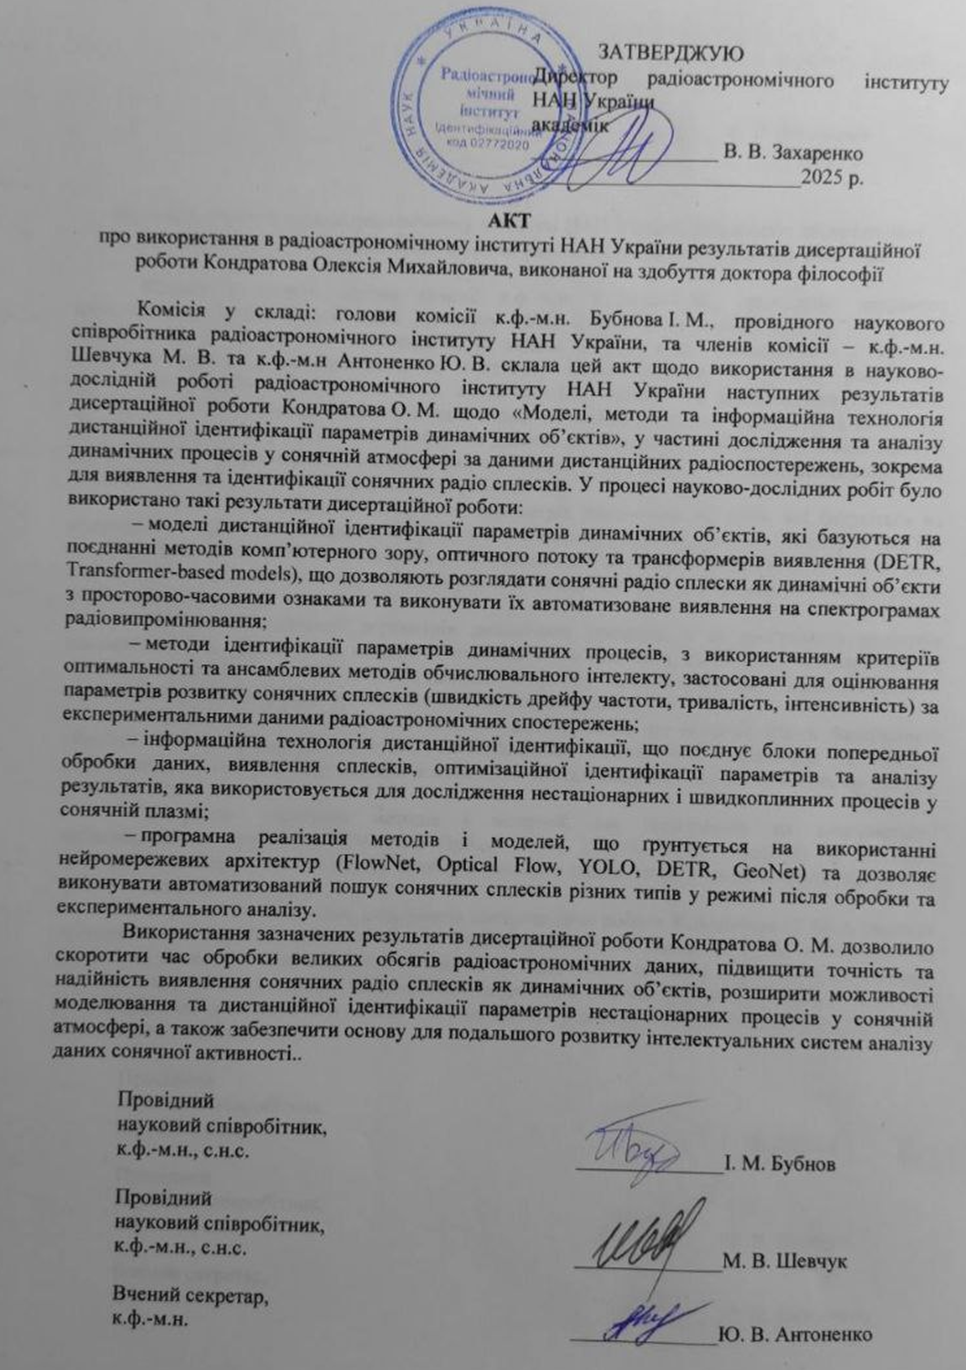
\includegraphics[width=6.4375in,height=9.13585in]{media/image56.png}

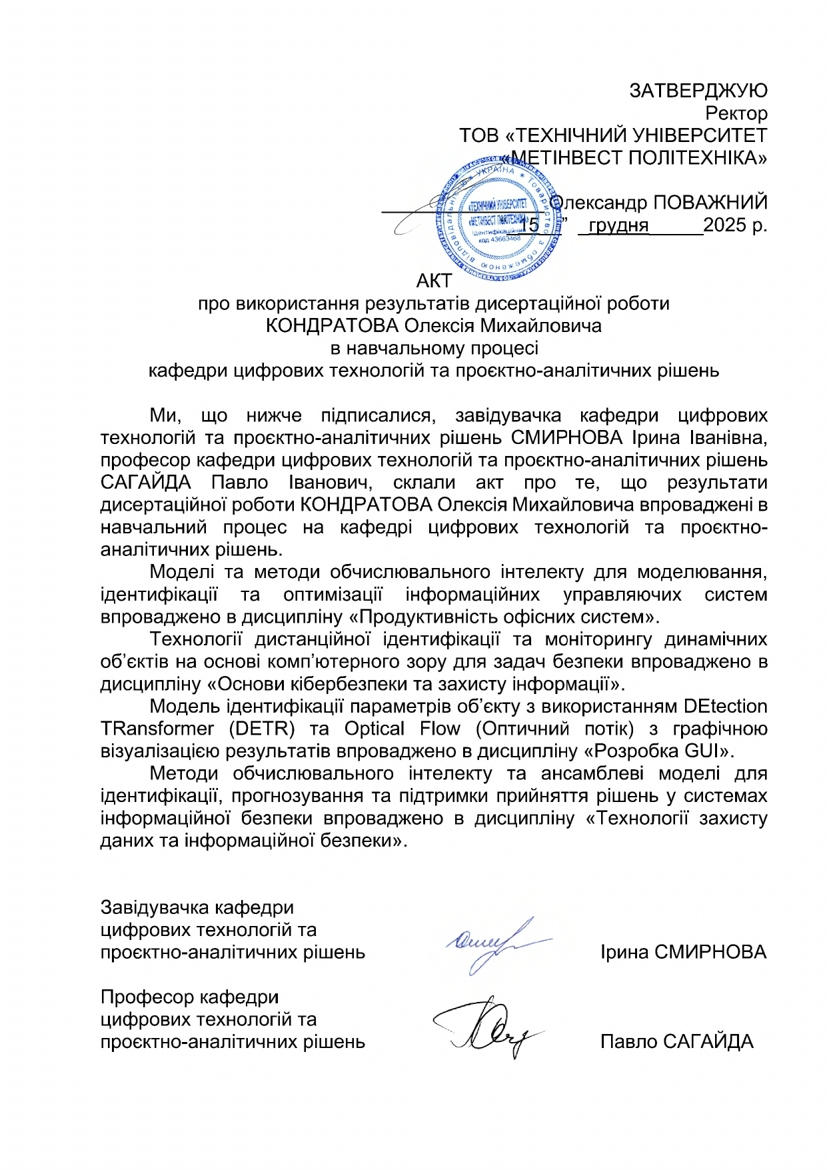
\includegraphics[width=6.6875in,height=9.45833in]{media/image57.jpeg}

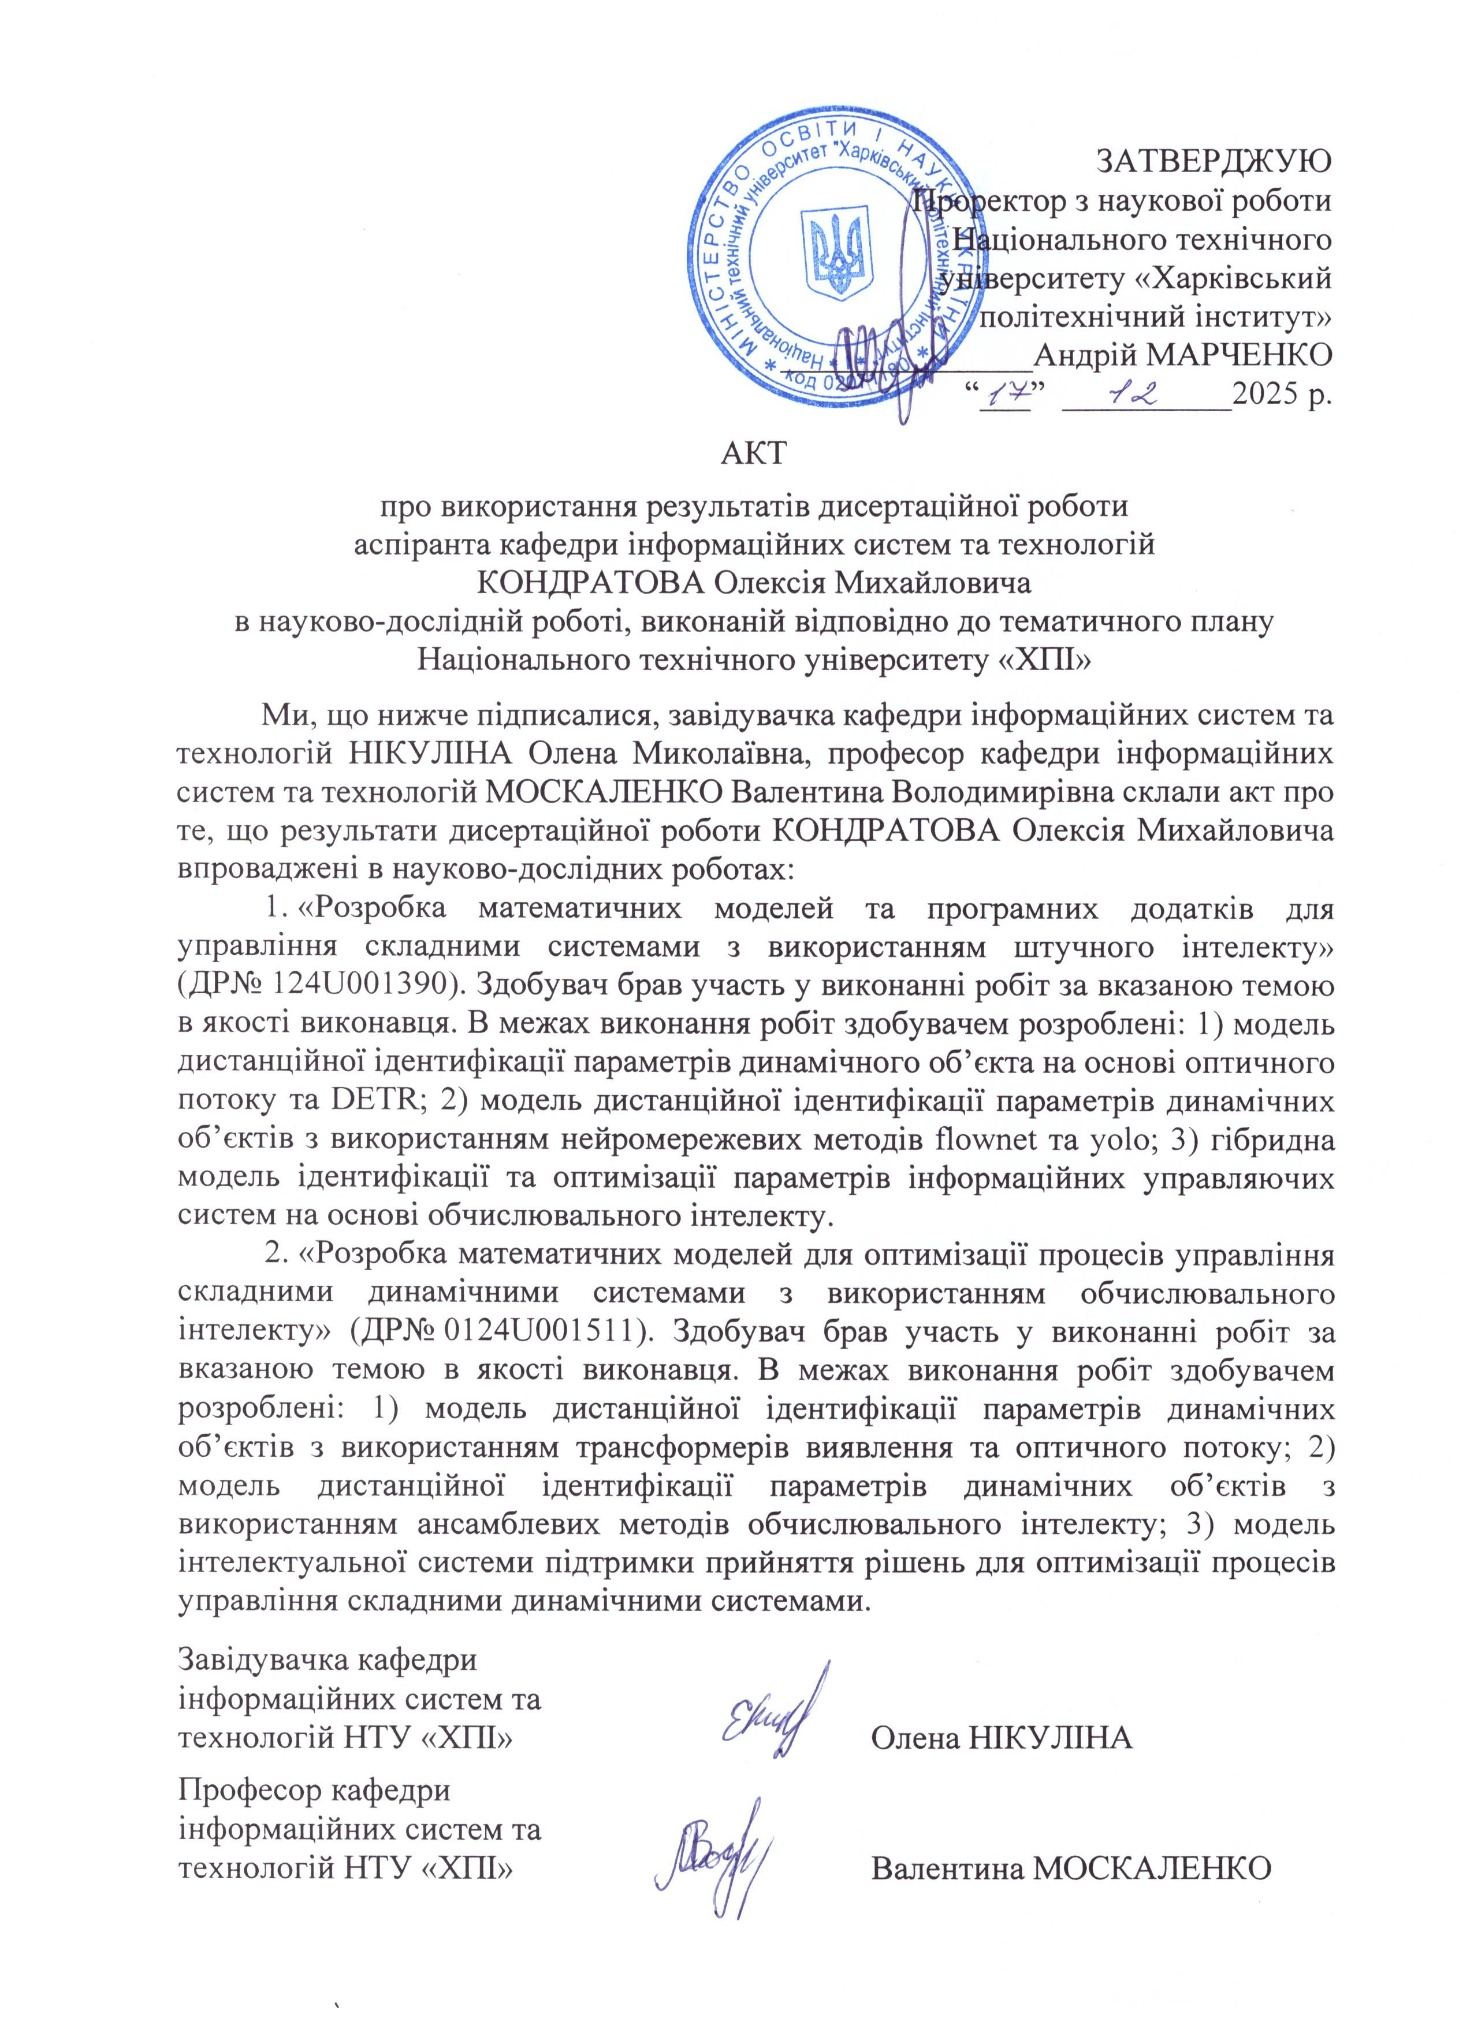
\includegraphics[width=6.69306in,height=9.2in]{media/image58.jpeg}

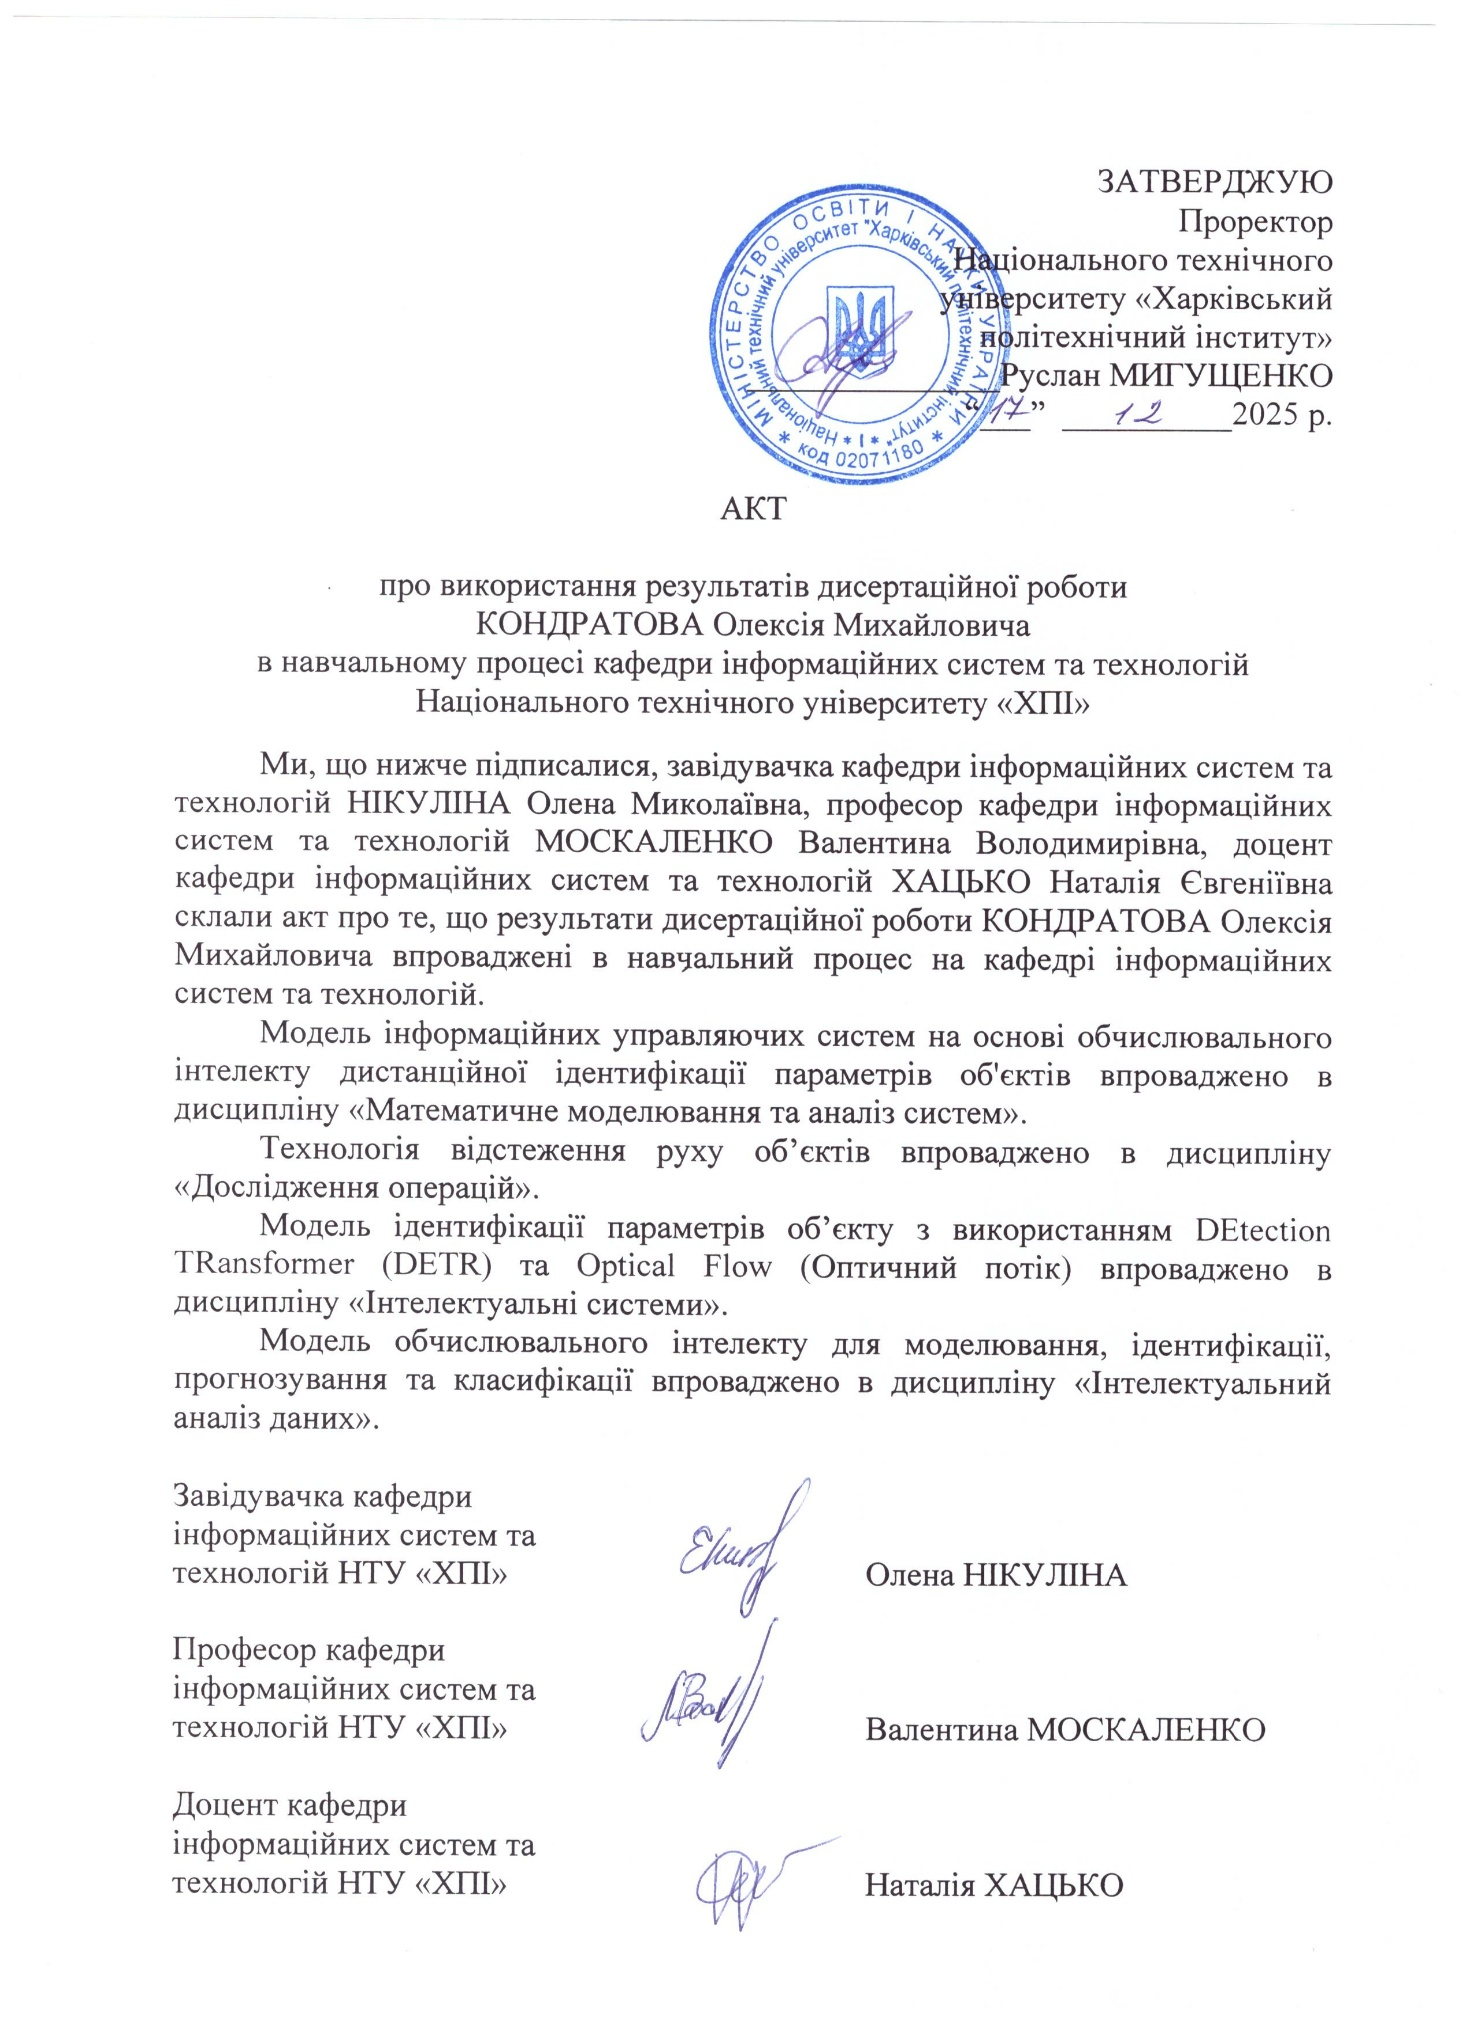
\includegraphics[width=6.69306in,height=9.2in]{media/image59.jpeg}
